%%%%%%%%%%%%%%%%%%%%%%%%%%%%%%%%%%%%%%%%%%%%%%%%%%%%%%%%%%%%%%%%%%%%%
%% Thesis master file
%% Alex Shires
%%%%%%%%%%%%%%%%%%%%%%%%%%%%%%%%%%%%%%%%%%%%%%%%%%%%%%%%%%%%%%%%%%%%%


\documentclass[12pt,a4paper,twoside]{report}


% Packages -------------------------------------------------
\usepackage[printonlyused]{acronym} % for linked acronyms
\usepackage{amsfonts}
\usepackage{amsmath}
\usepackage{amssymb}
\usepackage[toc,page]{appendix}
\usepackage{booktabs} % for nicer spacing between table lines
\usepackage{style/cancel} %to cancel terms in equations
\usepackage{caption}
\usepackage{cite} % to compress consecutive references, i.e. 1,2,3,4 -> 1-4
\usepackage{color} % for coloured text
\usepackage[nodayofweek]{datetime} % for date format customisation
\usepackage{enumitem} % for customisable lists
%\usepackage{fancyhdr} % for header/footer customisation
\usepackage[bottom]{footmisc} % to force footnotes to bottom of page
\usepackage{graphicx} % to include figures
%\usepackage{style/hepnames} % to include hep names
%\usepackage{style/hepparticles} % to include hep particles
%\usepackage{style/hepunits} % to include hep units %already in lhcb_symbols_def.tex (most of them)
\usepackage{ifthen} % for conditional statements
\usepackage{lineno} % for line numbering during review
\usepackage{mathtools} % for aligned matrices
%\usepackage{style/maybemath} % required for hep particles %needed??
\usepackage{multirow} % for table elements spanning multiple rows or columns
\usepackage{setspace} % to change line spacing
%\usepackage{style/SIunits} % to include SI units %already in lhcb_symbols_def.tex (most of them)
\usepackage{subfigure} % for figures within figures
%\usepackage[notlof,notlot,nottoc]{tocbibind} % for contents list without figures, tables or contents
\usepackage[nottoc]{tocbibind} % for contents list without figures, tables or contents
\usepackage{upgreek} % for upright lowercase greek letters
\usepackage{url} % for nicer urls \url{}
\usepackage{xspace} % for intelligent spacing after alias commands
\usepackage{alltt}
%\usepackage{quotation}
\usepackage{array}
%\usepackage{todonotes}
% Choose border size -----------------------------------------
\usepackage[margin=2.5cm]{geometry} % for screen
%\usepackage[margin=2.5cm, inner=2.9cm, outer=2.1cm]{geometry} % for bound copy
\usepackage{lscape}
\usepackage{pdfpages}
	

% Hyperlinks ------------------------------------------------
\usepackage{hyperref} % must be the last package loaded
\hypersetup{
 urlcolor=black, linkcolor=black, citecolor=black, colorlinks=true, % coloured text or surrounding box
 %linktoc=all, % contents list link: none, section, page, all
 % pdf viewer options
 pdftitle = {Exploring b to s electroweak penguin decays at LHCb},
 pdfauthor = {Alexander Shires},
 pdfstartpage=1, pdfstartview=FitV, pdfpagemode=UseOutlines, 
 bookmarksnumbered, bookmarksopen=true, bookmarksopenlevel=1,
}


% Aliases and defintions ---------------------------------------------------
\newboolean{articletitles}  %required in the bibliography
\setboolean{articletitles}{true}
\newboolean{uprightparticles}
\setboolean{uprightparticles}{false} %Set this to true to get roman particle symbols
%%% $Id: lhcb-symbols-def.tex 18993 2012-05-02 13:54:31Z uegede $
%%% ======================================================================
%%% Purpose: standard LHCb aliases
%%% Author: Originally Ulrik Egede, adapted by Tomasz Skwarnicki for templates,
%%% rewritten by Chris Parkes
%%% Created on: 2009-09-24
%%% =======================================================================

%%% this has to go before \begin{document}
%%%\usepackage{ifthen} 
%%%\newboolean{uprightparticles}
%%%\setboolean{uprightparticles}{true} %Set to false to get italic particle symbols

%%% Add comments with at least three %%% preceding.
%%% Add new sections with one % preceding
%%% Add new subsections with two %% preceding

%%%%%%%%%%%%%
% Experiments
%%%%%%%%%%%%%
\def\lhcb {\mbox{LHCb}\xspace}
\def\ux85 {\mbox{UX85}\xspace}
\def\cern {\mbox{CERN}\xspace}
\def\lhc    {\mbox{LHC}\xspace}
\def\atlas  {\mbox{ATLAS}\xspace}
\def\cms    {\mbox{CMS}\xspace}
\def\babar  {\mbox{BaBar}\xspace}
\def\belle  {\mbox{Belle}\xspace}
\def\aleph  {\mbox{ALEPH}\xspace}
\def\delphi {\mbox{DELPHI}\xspace}
\def\opal   {\mbox{OPAL}\xspace}
\def\lthree {\mbox{L3}\xspace}
\def\lep    {\mbox{LEP}\xspace}
\def\cdf    {\mbox{CDF}\xspace}
\def\dzero  {\mbox{D0}\xspace}
\def\sld    {\mbox{SLD}\xspace}
\def\cleo   {\mbox{CLEO}\xspace}
\def\argus  {\mbox{ARGUS}\xspace}
\def\uaone  {\mbox{UA1}\xspace}
\def\uatwo  {\mbox{UA2}\xspace}
\def\tevatron {Tevatron\xspace}

%% LHCb sub-detectors and sub-systems

\def\pu     {PU\xspace}
\def\velo   {VELO\xspace}
\def\rich   {RICH\xspace}
\def\richone {RICH1\xspace}
\def\richtwo {RICH2\xspace}
\def\ttracker {TT\xspace}
\def\intr   {IT\xspace}
\def\st     {ST\xspace}
\def\ot     {OT\xspace}
\def\Tone   {T1\xspace}
\def\Ttwo   {T2\xspace}
\def\Tthree {T3\xspace}
\def\Mone   {M1\xspace}
\def\Mtwo   {M2\xspace}
\def\Mthree {M3\xspace}
\def\Mfour  {M4\xspace}
\def\Mfive  {M5\xspace}
\def\ecal   {ECAL\xspace}
\def\spd    {SPD\xspace}
\def\presh  {PS\xspace}
\def\hcal   {HCAL\xspace}
\def\bcm    {BCM\xspace}

\def\ode    {ODE\xspace}
\def\daq    {DAQ\xspace}
\def\tfc    {TFC\xspace}
\def\ecs    {ECS\xspace}
\def\lone   {L0\xspace}
\def\hlt    {HLT\xspace}
\def\hltone {HLT1\xspace}
\def\hlttwo {HLT2\xspace}

%%% Upright (not slanted) Particles

\ifthenelse{\boolean{uprightparticles}}%
{\def\Palpha      {\ensuremath{\upalpha}\xspace}
 \def\Pbeta       {\ensuremath{\upbeta}\xspace}
 \def\Pgamma      {\ensuremath{\upgamma}\xspace}                 
 \def\Pdelta      {\ensuremath{\updelta}\xspace}                 
 \def\Pepsilon    {\ensuremath{\upepsilon}\xspace}                 
 \def\Pvarepsilon {\ensuremath{\upvarepsilon}\xspace}                 
 \def\Pzeta       {\ensuremath{\upzeta}\xspace}                 
 \def\Peta        {\ensuremath{\upeta}\xspace}                 
 \def\Ptheta      {\ensuremath{\uptheta}\xspace}                 
 \def\Pvartheta   {\ensuremath{\upvartheta}\xspace}                 
 \def\Piota       {\ensuremath{\upiota}\xspace}                 
 \def\Pkappa      {\ensuremath{\upkappa}\xspace}                 
 \def\Plambda     {\ensuremath{\uplambda}\xspace}                 
 \def\Pmu         {\ensuremath{\upmu}\xspace}                 
 \def\Pnu         {\ensuremath{\upnu}\xspace}                 
 \def\Pxi         {\ensuremath{\upxi}\xspace}                 
 \def\Ppi         {\ensuremath{\uppi}\xspace}                 
 \def\Pvarpi      {\ensuremath{\upvarpi}\xspace}                 
 \def\Prho        {\ensuremath{\uprho}\xspace}                 
 \def\Pvarrho     {\ensuremath{\upvarrho}\xspace}                 
 \def\Ptau        {\ensuremath{\uptau}\xspace}                 
 \def\Pupsilon    {\ensuremath{\upupsilon}\xspace}                 
 \def\Pphi        {\ensuremath{\upphi}\xspace}                 
 \def\Pvarphi     {\ensuremath{\upvarphi}\xspace}                 
 \def\Pchi        {\ensuremath{\upchi}\xspace}                 
 \def\Ppsi        {\ensuremath{\uppsi}\xspace}                 
 \def\Pomega      {\ensuremath{\upomega}\xspace}                 

 \def\PDelta      {\ensuremath{\Delta}\xspace}                 
 \def\PXi      {\ensuremath{\Xi}\xspace}                 
 \def\PLambda      {\ensuremath{\Lambda}\xspace}                 
 \def\PSigma      {\ensuremath{\Sigma}\xspace}                 
 \def\POmega      {\ensuremath{\Omega}\xspace}                 
 \def\PUpsilon      {\ensuremath{\Upsilon}\xspace}                 
 
 %\mathchardef\Deltares="7101
 %\mathchardef\Xi="7104
 %\mathchardef\Lambda="7103
 %\mathchardef\Sigma="7106
 %\mathchardef\Omega="710A


 \def\PA      {\ensuremath{\mathrm{A}}\xspace}                 
 \def\PB      {\ensuremath{\mathrm{B}}\xspace}                 
 \def\PC      {\ensuremath{\mathrm{C}}\xspace}                 
 \def\PD      {\ensuremath{\mathrm{D}}\xspace}                 
 \def\PE      {\ensuremath{\mathrm{E}}\xspace}                 
 \def\PF      {\ensuremath{\mathrm{F}}\xspace}                 
 \def\PG      {\ensuremath{\mathrm{G}}\xspace}                 
 \def\PH      {\ensuremath{\mathrm{H}}\xspace}                 
 \def\PI      {\ensuremath{\mathrm{I}}\xspace}                 
 \def\PJ      {\ensuremath{\mathrm{J}}\xspace}                 
 \def\PK      {\ensuremath{\mathrm{K}}\xspace}                 
 \def\PL      {\ensuremath{\mathrm{L}}\xspace}                 
 \def\PM      {\ensuremath{\mathrm{M}}\xspace}                 
 \def\PN      {\ensuremath{\mathrm{N}}\xspace}                 
 \def\PO      {\ensuremath{\mathrm{O}}\xspace}                 
 \def\PP      {\ensuremath{\mathrm{P}}\xspace}                 
 \def\PQ      {\ensuremath{\mathrm{Q}}\xspace}                 
 \def\PR      {\ensuremath{\mathrm{R}}\xspace}                 
 \def\PS      {\ensuremath{\mathrm{S}}\xspace}                 
 \def\PT      {\ensuremath{\mathrm{T}}\xspace}                 
 \def\PU      {\ensuremath{\mathrm{U}}\xspace}                 
 \def\PV      {\ensuremath{\mathrm{V}}\xspace}                 
 \def\PW      {\ensuremath{\mathrm{W}}\xspace}                 
 \def\PX      {\ensuremath{\mathrm{X}}\xspace}                 
 \def\PY      {\ensuremath{\mathrm{Y}}\xspace}                 
 \def\PZ      {\ensuremath{\mathrm{Z}}\xspace}                 
 \def\Pa      {\ensuremath{\mathrm{a}}\xspace}                 
 \def\Pb      {\ensuremath{\mathrm{b}}\xspace}                 
 \def\Pc      {\ensuremath{\mathrm{c}}\xspace}                 
 \def\Pd      {\ensuremath{\mathrm{d}}\xspace}                 
 \def\Pe      {\ensuremath{\mathrm{e}}\xspace}                 
 \def\Pf      {\ensuremath{\mathrm{f}}\xspace}                 
 \def\Pg      {\ensuremath{\mathrm{g}}\xspace}                 
 \def\Ph      {\ensuremath{\mathrm{h}}\xspace}                 
 \def\Pi      {\ensuremath{\mathrm{i}}\xspace}                 
 \def\Pj      {\ensuremath{\mathrm{j}}\xspace}                 
 \def\Pk      {\ensuremath{\mathrm{k}}\xspace}                 
 \def\Pl      {\ensuremath{\mathrm{l}}\xspace}                 
 \def\Pm      {\ensuremath{\mathrm{m}}\xspace}                 
 \def\Pn      {\ensuremath{\mathrm{n}}\xspace}                 
 \def\Po      {\ensuremath{\mathrm{o}}\xspace}                 
 \def\Pp      {\ensuremath{\mathrm{p}}\xspace}                 
 \def\Pq      {\ensuremath{\mathrm{q}}\xspace}                 
 \def\Pr      {\ensuremath{\mathrm{r}}\xspace}                 
 \def\Ps      {\ensuremath{\mathrm{s}}\xspace}                 
 \def\Pt      {\ensuremath{\mathrm{t}}\xspace}                 
 \def\Pu      {\ensuremath{\mathrm{u}}\xspace}                 
 \def\Pv      {\ensuremath{\mathrm{v}}\xspace}                 
 \def\Pw      {\ensuremath{\mathrm{w}}\xspace}                 
 \def\Px      {\ensuremath{\mathrm{x}}\xspace}                 
 \def\Py      {\ensuremath{\mathrm{y}}\xspace}                 
 \def\Pz      {\ensuremath{\mathrm{z}}\xspace}                 
}
{\def\Palpha      {\ensuremath{\alpha}\xspace}
 \def\Pbeta       {\ensuremath{\beta}\xspace}
 \def\Pgamma      {\ensuremath{\gamma}\xspace}                 
 \def\Pdelta      {\ensuremath{\delta}\xspace}                 
 \def\Pepsilon    {\ensuremath{\epsilon}\xspace}                 
 \def\Pvarepsilon {\ensuremath{\varepsilon}\xspace}                 
 \def\Pzeta       {\ensuremath{\zeta}\xspace}                 
 \def\Peta        {\ensuremath{\eta}\xspace}                 
 \def\Ptheta      {\ensuremath{\theta}\xspace}                 
 \def\Pvartheta   {\ensuremath{\vartheta}\xspace}                 
 \def\Piota       {\ensuremath{\iota}\xspace}                 
 \def\Pkappa      {\ensuremath{\kappa}\xspace}                 
 \def\Plambda     {\ensuremath{\lambda}\xspace}                 
 \def\Pmu         {\ensuremath{\mu}\xspace}                 
 \def\Pnu         {\ensuremath{\nu}\xspace}                 
 \def\Pxi         {\ensuremath{\xi}\xspace}                 
 \def\Ppi         {\ensuremath{\pi}\xspace}                 
 \def\Pvarpi      {\ensuremath{\varpi}\xspace}                 
 \def\Prho        {\ensuremath{\rho}\xspace}                 
 \def\Pvarrho     {\ensuremath{\varrho}\xspace}                 
 \def\Ptau        {\ensuremath{\tau}\xspace}                 
 \def\Pupsilon    {\ensuremath{\upsilon}\xspace}                 
 \def\Pphi        {\ensuremath{\phi}\xspace}                 
 \def\Pvarphi     {\ensuremath{\varphi}\xspace}                 
 \def\Pchi        {\ensuremath{\chi}\xspace}                 
 \def\Ppsi        {\ensuremath{\psi}\xspace}                 
 \def\Pomega      {\ensuremath{\omega}\xspace}                 
 \mathchardef\PDelta="7101
 \mathchardef\PXi="7104
 \mathchardef\PLambda="7103
 \mathchardef\PSigma="7106
 \mathchardef\POmega="710A
 \mathchardef\PUpsilon="7107
 \def\PA      {\ensuremath{A}\xspace}                 
 \def\PB      {\ensuremath{B}\xspace}                 
 \def\PC      {\ensuremath{C}\xspace}                 
 \def\PD      {\ensuremath{D}\xspace}                 
 \def\PE      {\ensuremath{E}\xspace}                 
 \def\PF      {\ensuremath{F}\xspace}                 
 \def\PG      {\ensuremath{G}\xspace}                 
 \def\PH      {\ensuremath{H}\xspace}                 
 \def\PI      {\ensuremath{I}\xspace}                 
 \def\PJ      {\ensuremath{J}\xspace}                 
 \def\PK      {\ensuremath{K}\xspace}                 
 \def\PL      {\ensuremath{L}\xspace}                 
 \def\PM      {\ensuremath{M}\xspace}                 
 \def\PN      {\ensuremath{N}\xspace}                 
 \def\PO      {\ensuremath{O}\xspace}                 
 \def\PP      {\ensuremath{P}\xspace}                 
 \def\PQ      {\ensuremath{Q}\xspace}                 
 \def\PR      {\ensuremath{R}\xspace}                 
 \def\PS      {\ensuremath{S}\xspace}                 
 \def\PT      {\ensuremath{T}\xspace}                 
 \def\PU      {\ensuremath{U}\xspace}                 
 \def\PV      {\ensuremath{V}\xspace}                 
 \def\PW      {\ensuremath{W}\xspace}                 
 \def\PX      {\ensuremath{X}\xspace}                 
 \def\PY      {\ensuremath{Y}\xspace}                 
 \def\PZ      {\ensuremath{Z}\xspace}                 
 \def\Pa      {\ensuremath{a}\xspace}                 
 \def\Pb      {\ensuremath{b}\xspace}                 
 \def\Pc      {\ensuremath{c}\xspace}                 
 \def\Pd      {\ensuremath{d}\xspace}                 
 \def\Pe      {\ensuremath{e}\xspace}                 
 \def\Pf      {\ensuremath{f}\xspace}                 
 \def\Pg      {\ensuremath{g}\xspace}                 
 \def\Ph      {\ensuremath{h}\xspace}                 
 \def\Pi      {\ensuremath{i}\xspace}                 
 \def\Pj      {\ensuremath{j}\xspace}                 
 \def\Pk      {\ensuremath{k}\xspace}                 
 \def\Pl      {\ensuremath{l}\xspace}                 
 \def\Pm      {\ensuremath{m}\xspace}                 
 \def\Pn      {\ensuremath{n}\xspace}                 
 \def\Po      {\ensuremath{o}\xspace}                 
 \def\Pp      {\ensuremath{p}\xspace}                 
 \def\Pq      {\ensuremath{q}\xspace}                 
 \def\Pr      {\ensuremath{r}\xspace}                 
 \def\Ps      {\ensuremath{s}\xspace}                 
 \def\Pt      {\ensuremath{t}\xspace}                 
 \def\Pu      {\ensuremath{u}\xspace}                 
 \def\Pv      {\ensuremath{v}\xspace}                 
 \def\Pw      {\ensuremath{w}\xspace}                 
 \def\Px      {\ensuremath{x}\xspace}                 
 \def\Py      {\ensuremath{y}\xspace}                 
 \def\Pz      {\ensuremath{z}\xspace}                 
}

%%%%%%%%%%%%%%%%%%%%%%%%%%%%%%%%%%%%%%%%%%%%%%%
% Particles

%% Leptons

\let\emi\en
\def\electron   {\ensuremath{\Pe}\xspace}
\def\en         {\ensuremath{\Pe^-}\xspace}   % electron negative (\em is taken)
\def\ep         {\ensuremath{\Pe^+}\xspace}
\def\epm        {\ensuremath{\Pe^\pm}\xspace} 
\def\epem       {\ensuremath{\Pe^+\Pe^-}\xspace}
\def\ee         {\ensuremath{\Pe^-\Pe^-}\xspace}

\def\mmu        {\ensuremath{\Pmu}\xspace}
\def\mup        {\ensuremath{\Pmu^+}\xspace}
\def\mun        {\ensuremath{\Pmu^-}\xspace} % muon negative (\mum is taken)
\def\mumu       {\ensuremath{\Pmu^+\Pmu^-}\xspace}
\def\mtau       {\ensuremath{\Ptau}\xspace}

\def\taup       {\ensuremath{\Ptau^+}\xspace}
\def\taum       {\ensuremath{\Ptau^-}\xspace}
\def\tautau     {\ensuremath{\Ptau^+\Ptau^-}\xspace}

\def\ellm       {\ensuremath{\ell^-}\xspace}
\def\ellp       {\ensuremath{\ell^+}\xspace}
\def\ellell     {\ensuremath{\ell^+ \ell^-}\xspace}

\def\neu        {\ensuremath{\Pnu}\xspace}
\def\neub       {\ensuremath{\overline{\Pnu}}\xspace}
\def\nuenueb    {\ensuremath{\neu\neub}\xspace}
\def\neue       {\ensuremath{\neu_e}\xspace}
\def\neueb      {\ensuremath{\neub_e}\xspace}
\def\neueneueb  {\ensuremath{\neue\neueb}\xspace}
\def\neum       {\ensuremath{\neu_\mu}\xspace}
\def\neumb      {\ensuremath{\neub_\mu}\xspace}
\def\neumneumb  {\ensuremath{\neum\neumb}\xspace}
\def\neut       {\ensuremath{\neu_\tau}\xspace}
\def\neutb      {\ensuremath{\neub_\tau}\xspace}
\def\neutneutb  {\ensuremath{\neut\neutb}\xspace}
\def\neul       {\ensuremath{\neu_\ell}\xspace}
\def\neulb      {\ensuremath{\neub_\ell}\xspace}
\def\neulneulb  {\ensuremath{\neul\neulb}\xspace}

%% Gauge bosons and scalars

\def\g      {\ensuremath{\Pgamma}\xspace}
\def\H      {\ensuremath{\PH^0}\xspace}
\def\Hp     {\ensuremath{\PH^+}\xspace}
\def\Hm     {\ensuremath{\PH^-}\xspace}
\def\Hpm    {\ensuremath{\PH^\pm}\xspace}
\def\W      {\ensuremath{\PW}\xspace}
\def\Wp     {\ensuremath{\PW^+}\xspace}
\def\Wm     {\ensuremath{\PW^-}\xspace}
\def\Wpm    {\ensuremath{\PW^\pm}\xspace}
\def\Z      {\ensuremath{\PZ^0}\xspace}

%% Quarks

\def\quark     {\ensuremath{\Pq}\xspace}
\def\quarkbar  {\ensuremath{\overline \quark}\xspace}
\def\qqbar     {\ensuremath{\quark\quarkbar}\xspace}
\def\uquark    {\ensuremath{\Pu}\xspace}
\def\uquarkbar {\ensuremath{\overline \uquark}\xspace}
\def\uubar     {\ensuremath{\uquark\uquarkbar}\xspace}
\def\dquark    {\ensuremath{\Pd}\xspace}
\def\dquarkbar {\ensuremath{\overline \dquark}\xspace}
\def\ddbar     {\ensuremath{\dquark\dquarkbar}\xspace}
\def\squark    {\ensuremath{\Ps}\xspace}
\def\squarkbar {\ensuremath{\overline \squark}\xspace}
\def\ssbar     {\ensuremath{\squark\squarkbar}\xspace}
\def\cquark    {\ensuremath{\Pc}\xspace}
\def\cquarkbar {\ensuremath{\overline \cquark}\xspace}
\def\ccbar     {\ensuremath{\cquark\cquarkbar}\xspace}
\def\bquark    {\ensuremath{\Pb}\xspace}
\def\bquarkbar {\ensuremath{\overline \bquark}\xspace}
\def\bbbar     {\ensuremath{\bquark\bquarkbar}\xspace}
\def\tquark    {\ensuremath{\Pt}\xspace}
\def\tquarkbar {\ensuremath{\overline \tquark}\xspace}
\def\ttbar     {\ensuremath{\tquark\tquarkbar}\xspace}

%% Light mesons

\def\pion  {\ensuremath{\Ppi}\xspace}
\def\piz   {\ensuremath{\pion^0}\xspace}
\def\pizs  {\ensuremath{\pion^0\mbox\,\rm{s}}\xspace}
\def\ppz   {\ensuremath{\pion^0\pion^0}\xspace}
\def\pip   {\ensuremath{\pion^+}\xspace}
\def\pim   {\ensuremath{\pion^-}\xspace}
\def\pipi  {\ensuremath{\pion^+\pion^-}\xspace}
\def\pipm  {\ensuremath{\pion^\pm}\xspace}
\def\pimp  {\ensuremath{\pion^\mp}\xspace}

\def\kaon  {\ensuremath{\PK}\xspace}
%%% do NOT use ensuremath here
  \def\Kbar  {\kern 0.2em\overline{\kern -0.2em \PK}{}\xspace}
\def\Kb    {\ensuremath{\Kbar}\xspace}
\def\Kz    {\ensuremath{\kaon^0}\xspace}
\def\Kzb   {\ensuremath{\Kbar^0}\xspace}
\def\KzKzb {\ensuremath{\Kz \kern -0.16em \Kzb}\xspace}
\def\Kp    {\ensuremath{\kaon^+}\xspace}
\def\Km    {\ensuremath{\kaon^-}\xspace}
\def\Kpm   {\ensuremath{\kaon^\pm}\xspace}
\def\Kmp   {\ensuremath{\kaon^\mp}\xspace}
\def\KpKm  {\ensuremath{\Kp \kern -0.16em \Km}\xspace}
\def\KS    {\ensuremath{\kaon^0_{\rm\scriptscriptstyle S}}\xspace} 
\def\KL    {\ensuremath{\kaon^0_{\rm\scriptscriptstyle L}}\xspace} 
\def\Kstarz  {\ensuremath{\kaon^{*0}}\xspace}
\def\Kstarzb {\ensuremath{\Kbar^{*0}}\xspace}
\def\Kstar   {\ensuremath{\kaon^*}\xspace}
\def\Kstarb  {\ensuremath{\Kbar^*}\xspace}
\def\Kstarp  {\ensuremath{\kaon^{*+}}\xspace}
\def\Kstarm  {\ensuremath{\kaon^{*-}}\xspace}
\def\Kstarpm {\ensuremath{\kaon^{*\pm}}\xspace}
\def\Kstarmp {\ensuremath{\kaon^{*\mp}}\xspace}

\newcommand{\etapr}{\ensuremath{\Peta^{\prime}}\xspace}

%% Heavy mesons

%%% do NOT use ensuremath here
  \def\Dbar    {\kern 0.2em\overline{\kern -0.2em \PD}{}\xspace}
\def\D       {\ensuremath{\PD}\xspace}
\def\Db      {\ensuremath{\Dbar}\xspace}
\def\Dz      {\ensuremath{\D^0}\xspace}
\def\Dzb     {\ensuremath{\Dbar^0}\xspace}
\def\DzDzb   {\ensuremath{\Dz {\kern -0.16em \Dzb}}\xspace}
\def\Dp      {\ensuremath{\D^+}\xspace}
\def\Dm      {\ensuremath{\D^-}\xspace}
\def\Dpm     {\ensuremath{\D^\pm}\xspace}
\def\Dmp     {\ensuremath{\D^\mp}\xspace}
\def\DpDm    {\ensuremath{\Dp {\kern -0.16em \Dm}}\xspace}
\def\Dstar   {\ensuremath{\D^*}\xspace}
\def\Dstarb  {\ensuremath{\Dbar^*}\xspace}
\def\Dstarz  {\ensuremath{\D^{*0}}\xspace}
\def\Dstarzb {\ensuremath{\Dbar^{*0}}\xspace}
\def\Dstarp  {\ensuremath{\D^{*+}}\xspace}
\def\Dstarm  {\ensuremath{\D^{*-}}\xspace}
\def\Dstarpm {\ensuremath{\D^{*\pm}}\xspace}
\def\Dstarmp {\ensuremath{\D^{*\mp}}\xspace}
\def\Ds      {\ensuremath{\D^+_\squark}\xspace}
\def\Dsp     {\ensuremath{\D^+_\squark}\xspace}
\def\Dsm     {\ensuremath{\D^-_\squark}\xspace}
\def\Dspm    {\ensuremath{\D^{\pm}_\squark}\xspace}
\def\Dss     {\ensuremath{\D^{*+}_\squark}\xspace}
\def\Dssp    {\ensuremath{\D^{*+}_\squark}\xspace}
\def\Dssm    {\ensuremath{\D^{*-}_\squark}\xspace}
\def\Dsspm   {\ensuremath{\D^{*\pm}_\squark}\xspace}

\def\B       {\ensuremath{\PB}\xspace}
%%% do NOT use ensuremath here
  \def\Bbar    {\kern 0.18em\overline{\kern -0.18em \PB}{}\xspace}
\def\Bb      {\ensuremath{\Bbar}\xspace}
\def\BBbar   {\ensuremath{\B\Bbar}\xspace} 
\def\Bz      {\ensuremath{\B^0}\xspace}
\def\Bzb     {\ensuremath{\Bbar^0}\xspace}
\def\Bu      {\ensuremath{\B^+}\xspace}
\def\Bub     {\ensuremath{\B^-}\xspace}
\def\Bp      {\ensuremath{\Bu}\xspace}
\def\Bm      {\ensuremath{\Bub}\xspace}
\def\Bpm     {\ensuremath{\B^\pm}\xspace}
\def\Bmp     {\ensuremath{\B^\mp}\xspace}
\def\Bd      {\ensuremath{\B^0}\xspace}
\def\Bs      {\ensuremath{\B^0_\squark}\xspace}
\def\Bsb     {\ensuremath{\Bbar^0_\squark}\xspace}
\def\Bdb     {\ensuremath{\Bbar^0}\xspace}
\def\Bc      {\ensuremath{\B_\cquark^+}\xspace}
\def\Bcp     {\ensuremath{\B_\cquark^+}\xspace}
\def\Bcm     {\ensuremath{\B_\cquark^-}\xspace}
\def\Bcpm    {\ensuremath{\B_\cquark^\pm}\xspace}

%% Onia

\def\jpsi     {\ensuremath{{\PJ\mskip -3mu/\mskip -2mu\Ppsi\mskip 2mu}}\xspace}
\def\psitwos  {\ensuremath{\Ppsi{(2S)}}\xspace}
\def\psiprpr  {\ensuremath{\Ppsi(3770)}\xspace}
\def\etac     {\ensuremath{\Peta_\cquark}\xspace}
\def\chiczero {\ensuremath{\Pchi_{\cquark 0}}\xspace}
\def\chicone  {\ensuremath{\Pchi_{\cquark 1}}\xspace}
\def\chictwo  {\ensuremath{\Pchi_{\cquark 2}}\xspace}
  %\mathchardef\Upsilon="7107
  \def\Y#1S{\ensuremath{\PUpsilon{(#1S)}}\xspace}% no space before {...}!
\def\OneS  {\Y1S}
\def\TwoS  {\Y2S}
\def\ThreeS{\Y3S}
\def\FourS {\Y4S}
\def\FiveS {\Y5S}

\def\chic  {\ensuremath{\Pchi_{c}}\xspace}

%% Baryons

\def\proton      {\ensuremath{\Pp}\xspace}
\def\antiproton  {\ensuremath{\overline \proton}\xspace}
\def\neutron     {\ensuremath{\Pn}\xspace}
\def\antineutron {\ensuremath{\overline \neutron}\xspace}

\def\Deltares {\ensuremath{\PDelta}\xspace}
\def\Deltaresbar{\ensuremath{\overline \Deltares}\xspace}
\def\Xires {\ensuremath{\PXi}\xspace}
\def\Xiresbar{\ensuremath{\overline \Xires}\xspace}
\def\L {\ensuremath{\PLambda}\xspace}
\def\Lbar {\ensuremath{\kern 0.1em\overline{\kern -0.1em\PLambda}}\xspace}
\def\Lambdares {\ensuremath{\PLambda}\xspace}
\def\Lambdaresbar{\ensuremath{\Lbar}\xspace}
\def\Sigmares {\ensuremath{\PSigma}\xspace}
\def\Sigmaresbar{\ensuremath{\overline \Sigmares}\xspace}
\def\Omegares {\ensuremath{\POmega}\xspace}
\def\Omegaresbar{\ensuremath{\overline \Omegares}\xspace}

%%% do NOT use ensuremath here
 % \def\Deltabar{\kern 0.25em\overline{\kern -0.25em \Deltares}{}\xspace}
 % \def\Sigbar{\kern 0.2em\overline{\kern -0.2em \Sigma}{}\xspace}
 % \def\Xibar{\kern 0.2em\overline{\kern -0.2em \Xi}{}\xspace}
 % \def\Obar{\kern 0.2em\overline{\kern -0.2em \Omega}{}\xspace}
 % \def\Nbar{\kern 0.2em\overline{\kern -0.2em N}{}\xspace}
 % \def\Xb{\kern 0.2em\overline{\kern -0.2em X}{}\xspace}

\def\Lb      {\ensuremath{\L^0_\bquark}\xspace}
\def\Lbbar   {\ensuremath{\Lbar^0_\bquark}\xspace}
\def\Lc      {\ensuremath{\L^+_\cquark}\xspace}
\def\Lcbar   {\ensuremath{\Lbar^-_\cquark}\xspace}

%%%%%%%%%%%%%%%%%%
% Physics symbols
%%%%%%%%%%%%%%%%%

%% Decays
\def\BF         {{\ensuremath{\cal B}\xspace}}
\def\BRvis      {{\ensuremath{\BR_{\rm{vis}}}}}
\def\BR         {\BF}
\newcommand{\decay}[2]{\ensuremath{#1\!\to #2}\xspace}         % {\Pa}{\Pb \Pc}
\def\ra                 {\ensuremath{\rightarrow}\xspace}
\def\to                 {\ensuremath{\rightarrow}\xspace}

%% Lifetimes
\newcommand{\tauBs}{\ensuremath{\tau_{\Bs}}\xspace}
\newcommand{\tauBd}{\ensuremath{\tau_{\Bd}}\xspace}
\newcommand{\tauBz}{\ensuremath{\tau_{\Bz}}\xspace}
\newcommand{\tauBu}{\ensuremath{\tau_{\Bp}}\xspace}
\newcommand{\tauDp}{\ensuremath{\tau_{\Dp}}\xspace}
\newcommand{\tauDz}{\ensuremath{\tau_{\Dz}}\xspace}
\newcommand{\tauL}{\ensuremath{\tau_{\rm L}}\xspace}
\newcommand{\tauH}{\ensuremath{\tau_{\rm H}}\xspace}

%% Masses
\newcommand{\mBd}{\ensuremath{m_{\Bd}}\xspace}
\newcommand{\mBp}{\ensuremath{m_{\Bp}}\xspace}
\newcommand{\mBs}{\ensuremath{m_{\Bs}}\xspace}
\newcommand{\mBc}{\ensuremath{m_{\Bc}}\xspace}
\newcommand{\mLb}{\ensuremath{m_{\Lb}}\xspace}

%% EW theory, groups
\def\grpsuthree {\ensuremath{\mathrm{SU}(3)}\xspace}
\def\grpsutw    {\ensuremath{\mathrm{SU}(2)}\xspace}
\def\grpuone    {\ensuremath{\mathrm{U}(1)}\xspace}

\def\ssqtw {\ensuremath{\sin^{2}\!\theta_{\mathrm{W}}}\xspace}
\def\csqtw {\ensuremath{\cos^{2}\!\theta_{\mathrm{W}}}\xspace}
\def\stw   {\ensuremath{\sin\theta_{\mathrm{W}}}\xspace}
\def\ctw   {\ensuremath{\cos\theta_{\mathrm{W}}}\xspace}
\def\ssqtwef {\ensuremath{{\sin}^{2}\theta_{\mathrm{W}}^{\mathrm{eff}}}\xspace}
\def\csqtwef {\ensuremath{{\cos}^{2}\theta_{\mathrm{W}}^{\mathrm{eff}}}\xspace}
\def\stwef {\ensuremath{\sin\theta_{\mathrm{W}}^{\mathrm{eff}}}\xspace}
\def\ctwef {\ensuremath{\cos\theta_{\mathrm{W}}^{\mathrm{eff}}}\xspace}
\def\gv    {\ensuremath{g_{\mbox{\tiny V}}}\xspace}
\def\ga    {\ensuremath{g_{\mbox{\tiny A}}}\xspace}

\def\order   {\ensuremath{\mathcal{O}}\xspace}
\def\ordalph {\ensuremath{\mathcal{O}(\alpha)}\xspace}
\def\ordalsq {\ensuremath{\mathcal{O}(\alpha^{2})}\xspace}
\def\ordalcb {\ensuremath{\mathcal{O}(\alpha^{3})}\xspace}

%% QCD parameters
\newcommand{\as}{\ensuremath{\alpha_{\scriptscriptstyle S}}\xspace}
\newcommand{\MSb}{\ensuremath{\overline{\mathrm{MS}}}\xspace}
\newcommand{\lqcd}{\ensuremath{\Lambda_{\mathrm{QCD}}}\xspace}
\def\qsq       {\ensuremath{q^2}\xspace}

%% CKM, CP violation

\def\eps   {\ensuremath{\varepsilon}\xspace}
\def\epsK  {\ensuremath{\varepsilon_K}\xspace}
\def\epsB  {\ensuremath{\varepsilon_B}\xspace}
\def\epsp  {\ensuremath{\varepsilon^\prime_K}\xspace}

\def\CP                {\ensuremath{C\!P}\xspace}
\def\CPT               {\ensuremath{C\!PT}\xspace}

\def\rhobar {\ensuremath{\overline \rho}\xspace}
\def\etabar {\ensuremath{\overline \eta}\xspace}

\def\Vud  {\ensuremath{|V_{\uquark\dquark}|}\xspace}
\def\Vcd  {\ensuremath{|V_{\cquark\dquark}|}\xspace}
\def\Vtd  {\ensuremath{|V_{\tquark\dquark}|}\xspace}
\def\Vus  {\ensuremath{|V_{\uquark\squark}|}\xspace}
\def\Vcs  {\ensuremath{|V_{\cquark\squark}|}\xspace}
\def\Vts  {\ensuremath{|V_{\tquark\squark}|}\xspace}
\def\Vub  {\ensuremath{|V_{\uquark\bquark}|}\xspace}
\def\Vcb  {\ensuremath{|V_{\cquark\bquark}|}\xspace}
\def\Vtb  {\ensuremath{|V_{\tquark\bquark}|}\xspace}

%% Oscillations

\newcommand{\dm}{\ensuremath{\Delta m}\xspace}
\newcommand{\dms}{\ensuremath{\Delta m_{\squark}}\xspace}
\newcommand{\dmd}{\ensuremath{\Delta m_{\dquark}}\xspace}
\newcommand{\DG}{\ensuremath{\Delta\Gamma}\xspace}
\newcommand{\DGs}{\ensuremath{\Delta\Gamma_{\squark}}\xspace}
\newcommand{\DGd}{\ensuremath{\Delta\Gamma_{\dquark}}\xspace}
\newcommand{\Gs}{\ensuremath{\Gamma_{\squark}}\xspace}
\newcommand{\Gd}{\ensuremath{\Gamma_{\dquark}}\xspace}

\newcommand{\MBq}{\ensuremath{M_{\B_\quark}}\xspace}
\newcommand{\DGq}{\ensuremath{\Delta\Gamma_{\quark}}\xspace}
\newcommand{\Gq}{\ensuremath{\Gamma_{\quark}}\xspace}
\newcommand{\dmq}{\ensuremath{\Delta m_{\quark}}\xspace}
\newcommand{\GL}{\ensuremath{\Gamma_{\rm L}}\xspace}
\newcommand{\GH}{\ensuremath{\Gamma_{\rm H}}\xspace}

\newcommand{\DGsGs}{\ensuremath{\Delta\Gamma_{\squark}/\Gamma_{\squark}}\xspace}
\newcommand{\Delm}{\mbox{$\Delta m $}\xspace}
\newcommand{\ACP}{\ensuremath{{\cal A}^{\CP}}\xspace}
\newcommand{\Adir}{\ensuremath{{\cal A}^{\rm dir}}\xspace}
\newcommand{\Amix}{\ensuremath{{\cal A}^{\rm mix}}\xspace}
\newcommand{\ADelta}{\ensuremath{{\cal A}^\Delta}\xspace}
\newcommand{\phid}{\ensuremath{\phi_{\dquark}}\xspace}
\newcommand{\sinphid}{\ensuremath{\sin\!\phid}\xspace}
\newcommand{\phis}{\ensuremath{\phi_{\squark}}\xspace}
\newcommand{\betas}{\ensuremath{\beta_{\squark}}\xspace}
\newcommand{\sbetas}{\ensuremath{\sigma(\beta_{\squark})}\xspace}
\newcommand{\stbetas}{\ensuremath{\sigma(2\beta_{\squark})}\xspace}
\newcommand{\stphis}{\ensuremath{\sigma(\phi_{\squark})}\xspace}
\newcommand{\sinphis}{\ensuremath{\sin\!\phis}\xspace}

%% Tagging
\newcommand{\edet}{{\ensuremath{\varepsilon_{\rm det}}}\xspace}
\newcommand{\erec}{{\ensuremath{\varepsilon_{\rm rec/det}}}\xspace}
\newcommand{\esel}{{\ensuremath{\varepsilon_{\rm sel/rec}}}\xspace}
\newcommand{\etrg}{{\ensuremath{\varepsilon_{\rm trg/sel}}}\xspace}
\newcommand{\etot}{{\ensuremath{\varepsilon_{\rm tot}}}\xspace}

\newcommand{\mistag}{\ensuremath{\omega}\xspace}
\newcommand{\wcomb}{\ensuremath{\omega^{\rm comb}}\xspace}
\newcommand{\etag}{{\ensuremath{\varepsilon_{\rm tag}}}\xspace}
\newcommand{\etagcomb}{{\ensuremath{\varepsilon_{\rm tag}^{\rm comb}}}\xspace}
\newcommand{\effeff}{\ensuremath{\varepsilon_{\rm eff}}\xspace}
\newcommand{\effeffcomb}{\ensuremath{\varepsilon_{\rm eff}^{\rm comb}}\xspace}
\newcommand{\efftag}{{\ensuremath{\etag(1-2\omega)^2}}\xspace}
\newcommand{\effD}{{\ensuremath{\etag D^2}}\xspace}

\newcommand{\etagprompt}{{\ensuremath{\varepsilon_{\rm tag}^{\rm Pr}}}\xspace}
\newcommand{\etagLL}{{\ensuremath{\varepsilon_{\rm tag}^{\rm LL}}}\xspace}

%% Key decay channels

\def\BdToKstmm    {\decay{\Bd}{\Kstarz\mup\mun}}
\def\BdbToKstmm   {\decay{\Bdb}{\Kstarzb\mup\mun}}

\def\BsToJPsiPhi  {\decay{\Bs}{\jpsi\phi}}
\def\BdToJPsiKst  {\decay{\Bd}{\jpsi\Kstarz}}
\def\BdbToJPsiKst {\decay{\Bdb}{\jpsi\Kstarzb}}

\def\BsPhiGam     {\decay{\Bs}{\phi \g}}
\def\BdKstGam     {\decay{\Bd}{\Kstarz \g}}

\def\BTohh        {\decay{\B}{\Ph^+ \Ph'^-}}
\def\BdTopipi     {\decay{\Bd}{\pip\pim}}
\def\BdToKpi      {\decay{\Bd}{\Kp\pim}}
\def\BsToKK       {\decay{\Bs}{\Kp\Km}}
\def\BsTopiK      {\decay{\Bs}{\pip\Km}}

%% Rare decays
\def\BdKstee  {\decay{\Bd}{\Kstarz\epem}}
\def\BdbKstee {\decay{\Bdb}{\Kstarzb\epem}}
\def\bsll     {\decay{\bquark}{\squark \ell^+ \ell^-}}
\def\AFB      {\ensuremath{A_{\mathrm{FB}}}\xspace}
\def\FL       {\ensuremath{F_{\mathrm{L}}}\xspace}
\def\AT#1     {\ensuremath{A_{\mathrm{T}}^{#1}}\xspace}           % 2
\def\btosgam  {\decay{\bquark}{\squark \g}}
\def\btodgam  {\decay{\bquark}{\dquark \g}}
\def\Bsmm     {\decay{\Bs}{\mup\mun}}
\def\Bdmm     {\decay{\Bd}{\mup\mun}}
\def\ctl       {\ensuremath{\cos{\theta_l}}\xspace}
\def\ctk       {\ensuremath{\cos{\theta_K}}\xspace}

%% Wilson coefficients and operators
\def\C#1      {\ensuremath{\mathcal{C}_{#1}}\xspace}                       % 9
\def\Cp#1     {\ensuremath{\mathcal{C}_{#1}^{'}}\xspace}                    % 7
\def\Ceff#1   {\ensuremath{\mathcal{C}_{#1}^{\mathrm{(eff)}}}\xspace}        % 9  
\def\Cpeff#1  {\ensuremath{\mathcal{C}_{#1}^{'\mathrm{(eff)}}}\xspace}       % 7
\def\Ope#1    {\ensuremath{\mathcal{O}_{#1}}\xspace}                       % 2
\def\Opep#1   {\ensuremath{\mathcal{O}_{#1}^{'}}\xspace}                    % 7

%% Charm

\def\xprime     {\ensuremath{x^{\prime}}\xspace}
\def\yprime     {\ensuremath{y^{\prime}}\xspace}
\def\ycp        {\ensuremath{y_{\CP}}\xspace}
\def\agamma     {\ensuremath{A_{\Gamma}}\xspace}
\def\kpi        {\ensuremath{\PK\Ppi}\xspace}
\def\kk         {\ensuremath{\PK\PK}\xspace}
\def\dkpi       {\decay{\PD}{\PK\Ppi}}
\def\dkk        {\decay{\PD}{\PK\PK}}
\def\dkpicf     {\decay{\Dz}{\Km\pip}}

%% QM
\newcommand{\bra}[1]{\ensuremath{\langle #1|}}             % {a}
\newcommand{\ket}[1]{\ensuremath{|#1\rangle}}              % {b}
\newcommand{\braket}[2]{\ensuremath{\langle #1|#2\rangle}} % {a}{b}

%%%%%%%%%%%%%%%%%%%%%%%%%%%%%%%%%%%%%%%%%%%%%%%%%%
% Units
%%%%%%%%%%%%%%%%%%%%%%%%%%%%%%%%%%%%%%%%%%%%%%%%%%
\newcommand{\unit}[1]{\ensuremath{\rm\,#1}\xspace}          % {kg}

%% Energy and momentum
\newcommand{\tev}{\ensuremath{\mathrm{\,Te\kern -0.1em V}}\xspace}
\newcommand{\gev}{\ensuremath{\mathrm{\,Ge\kern -0.1em V}}\xspace}
\newcommand{\mev}{\ensuremath{\mathrm{\,Me\kern -0.1em V}}\xspace}
\newcommand{\kev}{\ensuremath{\mathrm{\,ke\kern -0.1em V}}\xspace}
\newcommand{\ev}{\ensuremath{\mathrm{\,e\kern -0.1em V}}\xspace}
\newcommand{\gevc}{\ensuremath{{\mathrm{\,Ge\kern -0.1em V\!/}c}}\xspace}
\newcommand{\mevc}{\ensuremath{{\mathrm{\,Me\kern -0.1em V\!/}c}}\xspace}
\newcommand{\gevcc}{\ensuremath{{\mathrm{\,Ge\kern -0.1em V\!/}c^2}}\xspace}
\newcommand{\gevgevcccc}{\ensuremath{{\mathrm{\,Ge\kern -0.1em V^2\!/}c^4}}\xspace}
\newcommand{\mevcc}{\ensuremath{{\mathrm{\,Me\kern -0.1em V\!/}c^2}}\xspace}

%% Distance and area
\def\km   {\ensuremath{\rm \,km}\xspace}
\def\m    {\ensuremath{\rm \,m}\xspace}
\def\cm   {\ensuremath{\rm \,cm}\xspace}
\def\cma  {\ensuremath{{\rm \,cm}^2}\xspace}
\def\mm   {\ensuremath{\rm \,mm}\xspace}
\def\mma  {\ensuremath{{\rm \,mm}^2}\xspace}
\def\mum  {\ensuremath{\,\upmu\rm m}\xspace}
\def\muma {\ensuremath{\,\upmu\rm m^2}\xspace}
\def\nm   {\ensuremath{\rm \,nm}\xspace}
\def\fm   {\ensuremath{\rm \,fm}\xspace}
\def\barn{\ensuremath{\rm \,b}\xspace}
\def\barnhyph{\ensuremath{\rm -b}\xspace}
\def\mbarn{\ensuremath{\rm \,mb}\xspace}
\def\mub{\ensuremath{\rm \,\upmu b}\xspace}
\def\mbarnhyph{\ensuremath{\rm -mb}\xspace}
\def\nb {\ensuremath{\rm \,nb}\xspace}
\def\invnb {\ensuremath{\mbox{\,nb}^{-1}}\xspace}
\def\pb {\ensuremath{\rm \,pb}\xspace}
\def\invpb {\ensuremath{\mbox{\,pb}^{-1}}\xspace}
\def\fb   {\ensuremath{\mbox{\,fb}}\xspace}
\def\invfb   {\ensuremath{\mbox{\,fb}^{-1}}\xspace}

%% Time 
\def\sec  {\ensuremath{\rm {\,s}}\xspace}
\def\ms   {\ensuremath{{\rm \,ms}}\xspace}
\def\mus  {\ensuremath{\,\upmu{\rm s}}\xspace}
\def\ns   {\ensuremath{{\rm \,ns}}\xspace}
\def\ps   {\ensuremath{{\rm \,ps}}\xspace}
\def\fs   {\ensuremath{\rm \,fs}\xspace}

\def\mhz  {\ensuremath{{\rm \,MHz}}\xspace}
\def\khz  {\ensuremath{{\rm \,kHz}}\xspace}
\def\hz   {\ensuremath{{\rm \,Hz}}\xspace}

\def\invps{\ensuremath{{\rm \,ps^{-1}}}\xspace}

\def\yr   {\ensuremath{\rm \,yr}\xspace}
\def\hr   {\ensuremath{\rm \,hr}\xspace}

%% Temperature
\def\degc {\ensuremath{^\circ}{C}\xspace}
\def\degk {\ensuremath {\rm K}\xspace}

%% Material lengths, radiation
\def\Xrad {\ensuremath{X_0}\xspace}
\def\NIL{\ensuremath{\lambda_{int}}\xspace}
\def\mip {MIP\xspace}
\def\neutroneq {\ensuremath{\rm \,n_{eq}}\xspace}
\def\neqcmcm {\ensuremath{\rm \,n_{eq} / cm^2}\xspace}
\def\kRad {\ensuremath{\rm \,kRad}\xspace}
\def\MRad {\ensuremath{\rm \,MRad}\xspace}
\def\ci {\ensuremath{\rm \,Ci}\xspace}
\def\mci {\ensuremath{\rm \,mCi}\xspace}

%% Uncertainties
\def\sx    {\ensuremath{\sigma_x}\xspace}    
\def\sy    {\ensuremath{\sigma_y}\xspace}   
\def\sz    {\ensuremath{\sigma_z}\xspace}    

\newcommand{\stat}{\ensuremath{\mathrm{(stat)}}\xspace}
\newcommand{\syst}{\ensuremath{\mathrm{(syst)}}\xspace}

%% Maths

\def\order{{\ensuremath{\cal O}}\xspace}
\newcommand{\chisq}{\ensuremath{\chi^2}\xspace}

\def\deriv {\ensuremath{\mathrm{d}}}

\def\gsim{{~\raise.15em\hbox{$>$}\kern-.85em
          \lower.35em\hbox{$\sim$}~}\xspace}
\def\lsim{{~\raise.15em\hbox{$<$}\kern-.85em
          \lower.35em\hbox{$\sim$}~}\xspace}

\newcommand{\mean}[1]{\ensuremath{\left\langle #1 \right\rangle}} % {x}
\newcommand{\abs}[1]{\ensuremath{\left\|#1\right\|}} % {x}
\newcommand{\Real}{\ensuremath{\mathcal{R}e}\xspace}
\newcommand{\Imag}{\ensuremath{\mathcal{I}m}\xspace}

\def\PDF {PDF\xspace}

\def\sPlot{\mbox{\em sPlot}}
\def\sWeights{\mbox{\em sWeights}}
%%%%%%%%%%%%%%%%%%%%%%%%%%%%%%%%%%%%%%%%%%%%%%%%%%
% Kinematics
%%%%%%%%%%%%%%%%%%%%%%%%%%%%%%%%%%%%%%%%%%%%%%%%%%

%% Energy, Momenta
\def\Ebeam {\ensuremath{E_{\mbox{\tiny BEAM}}}\xspace}
\def\sqs   {\ensuremath{\protect\sqrt{s}}\xspace}

\def\ptot       {\mbox{$p$}\xspace}
\def\pt         {\mbox{$p_{\rm T}$}\xspace}
\def\et         {\mbox{$E_{\rm T}$}\xspace}
\def\dpp        {\ensuremath{\mathrm{d}\hspace{-0.1em}p/p}\xspace}

\newcommand{\dedx}{\ensuremath{\mathrm{d}\hspace{-0.1em}E/\mathrm{d}x}\xspace}

%% PID

\def\dllkpi     {\ensuremath{\mathrm{DLL}_{\kaon\pion}}\xspace}
\def\dllppi     {\ensuremath{\mathrm{DLL}_{\proton\pion}}\xspace}
\def\dllepi     {\ensuremath{\mathrm{DLL}_{\electron\pion}}\xspace}
\def\dllmupi    {\ensuremath{\mathrm{DLL}_{\mmu\pi}}\xspace}

%% Geometry
\def\mphi       {\mbox{$\phi$}\xspace}
\def\mtheta     {\mbox{$\theta$}\xspace}
\def\ctheta     {\mbox{$\cos\theta$}\xspace}
\def\stheta     {\mbox{$\sin\theta$}\xspace}
\def\ttheta     {\mbox{$\tan\theta$}\xspace}

\def\degrees{\ensuremath{^{\circ}}\xspace}
\def\krad {\ensuremath{\rm \,krad}\xspace}
\def\mrad{\ensuremath{\rm \,mrad}\xspace}
\def\rad{\ensuremath{\rm \,rad}\xspace}

%% Accelerator
\def\betastar {\ensuremath{\beta^*}}
\newcommand{\lum} {\ensuremath{\mathcal{L}}\xspace}
\newcommand{\intlum}[1]{\ensuremath{\int\lum=#1\xspace}}  % {2 \,\invfb}

%%%%%%%%%%%%%%%%%%%%%%%%%%%%%%%%%%%%%%%%%%%%%%%%%%%%%%%%%%%%%%%%%%%%
% Software
%%%%%%%%%%%%%%%%%%%%%%%%%%%%%%%%%%%%%%%%%%%%%%%%%%%%%%%%%%%%%%%%%%%%

%% Programs
\def\evtgen     {\mbox{\textsc{EvtGen}}\xspace}
\def\pythia     {\mbox{\textsc{Pythia}}\xspace}
\def\fluka      {\mbox{\textsc{Fluka}}\xspace}
\def\tosca      {\mbox{\textsc{Tosca}}\xspace}
\def\ansys      {\mbox{\textsc{Ansys}}\xspace}
\def\spice      {\mbox{\textsc{Spice}}\xspace}
\def\garfield   {\mbox{\textsc{Garfield}}\xspace}
\def\geant      {\mbox{\textsc{Geant4}}\xspace}
\def\hepmc      {\mbox{\textsc{HepMC}}\xspace}
\def\gauss      {\mbox{\textsc{Gauss}}\xspace}
\def\gaudi      {\mbox{\textsc{Gaudi}}\xspace}
\def\boole      {\mbox{\textsc{Boole}}\xspace}
\def\brunel     {\mbox{\textsc{Brunel}}\xspace}
\def\davinci    {\mbox{\textsc{DaVinci}}\xspace}
\def\erasmus    {\mbox{\textsc{Erasmus}}\xspace}
\def\moore      {\mbox{\textsc{Moore}}\xspace}
\def\ganga      {\mbox{\textsc{Ganga}}\xspace}
\def\dirac      {\mbox{\textsc{Dirac}}\xspace}
\def\root       {\mbox{\textsc{Root}}\xspace}
\def\roofit     {\mbox{\textsc{RooFit}}\xspace}
\def\pyroot     {\mbox{\textsc{PyRoot}}\xspace}
\def\photos     {\mbox{\textsc{Photos}}\xspace}

%% Languages
\def\cpp        {\mbox{\textsc{C\raisebox{0.1em}{{\footnotesize{++}}}}}\xspace}
\def\python     {\mbox{\textsc{Python}}\xspace}
\def\ruby       {\mbox{\textsc{Ruby}}\xspace}
\def\fortran    {\mbox{\textsc{Fortran}}\xspace}
\def\svn        {\mbox{\textsc{SVN}}\xspace}

%% Data processing
\def\kbytes     {\ensuremath{{\rm \,kbytes}}\xspace}
\def\kbsps      {\ensuremath{{\rm \,kbytes/s}}\xspace}
\def\kbits      {\ensuremath{{\rm \,kbits}}\xspace}
\def\kbsps      {\ensuremath{{\rm \,kbits/s}}\xspace}
\def\mbsps      {\ensuremath{{\rm \,Mbits/s}}\xspace}
\def\mbytes     {\ensuremath{{\rm \,Mbytes}}\xspace}
\def\mbps       {\ensuremath{{\rm \,Mbyte/s}}\xspace}
\def\mbsps      {\ensuremath{{\rm \,Mbytes/s}}\xspace}
\def\gbsps      {\ensuremath{{\rm \,Gbits/s}}\xspace}
\def\gbytes     {\ensuremath{{\rm \,Gbytes}}\xspace}
\def\gbsps      {\ensuremath{{\rm \,Gbytes/s}}\xspace}
\def\tbytes     {\ensuremath{{\rm \,Tbytes}}\xspace}
\def\tbpy       {\ensuremath{{\rm \,Tbytes/yr}}\xspace}

\def\dst        {DST\xspace}

%%%%%%%%%%%%%%%%%%%%%%%%%%%
% Detector related
%%%%%%%%%%%%%%%%%%%%%%%%%%%

%% Detector technologies
\def\nonn {\ensuremath{\rm {\it{n^+}}\mbox{-}on\mbox{-}{\it{n}}}\xspace}
\def\ponn {\ensuremath{\rm {\it{p^+}}\mbox{-}on\mbox{-}{\it{n}}}\xspace}
\def\nonp {\ensuremath{\rm {\it{n^+}}\mbox{-}on\mbox{-}{\it{p}}}\xspace}
\def\cvd  {CVD\xspace}
\def\mwpc {MWPC\xspace}
\def\gem  {GEM\xspace}

%% Detector components, electronics
\def\tell1  {TELL1\xspace}
\def\ukl1   {UKL1\xspace}
\def\beetle {Beetle\xspace}
\def\otis   {OTIS\xspace}
\def\croc   {CROC\xspace}
\def\carioca {CARIOCA\xspace}
\def\dialog {DIALOG\xspace}
\def\sync   {SYNC\xspace}
\def\cardiac {CARDIAC\xspace}
\def\gol    {GOL\xspace}
\def\vcsel  {VCSEL\xspace}
\def\ttc    {TTC\xspace}
\def\ttcrx  {TTCrx\xspace}
\def\hpd    {HPD\xspace}
\def\pmt    {PMT\xspace}
\def\specs  {SPECS\xspace}
\def\elmb   {ELMB\xspace}
\def\fpga   {FPGA\xspace}
\def\plc    {PLC\xspace}
\def\rasnik {RASNIK\xspace}
\def\elmb   {ELMB\xspace}
\def\can    {CAN\xspace}
\def\lvds   {LVDS\xspace}
\def\ntc    {NTC\xspace}
\def\adc    {ADC\xspace}
\def\led    {LED\xspace}
\def\ccd    {CCD\xspace}
\def\hv     {HV\xspace}
\def\lv     {LV\xspace}
\def\pvss   {PVSS\xspace}
\def\cmos   {CMOS\xspace}
\def\fifo   {FIFO\xspace}
\def\ccpc   {CCPC\xspace}

%% Chemical symbols
\def\cfourften     {\ensuremath{\rm C_4 F_{10}}\xspace}
\def\cffour        {\ensuremath{\rm CF_4}\xspace}
\def\cotwo         {\ensuremath{\rm CO_2}\xspace} 
\def\csixffouteen  {\ensuremath{\rm C_6 F_{14}}\xspace} 
\def\mgftwo     {\ensuremath{\rm Mg F_2}\xspace} 
\def\siotwo     {\ensuremath{\rm SiO_2}\xspace} 

%%%%%%%%%%%%%%%
% Special Text 
%%%%%%%%%%%%%%%
\newcommand{\eg}{\mbox{\itshape e.g.}\xspace}
\newcommand{\ie}{\mbox{\itshape i.e.}}
\newcommand{\etal}{{\slshape et al.\/}\xspace}
\newcommand{\etc}{\mbox{\itshape etc.}\xspace}
\newcommand{\cf}{\mbox{\itshape cf.}\xspace}
\newcommand{\ffp}{\mbox{\itshape ff.}\xspace}
 % lhcb standard file
%%%% $Id: lhcb-symbols-def.tex 1903 2011-02-03 18:49:28Z cblanks $
%%% ======================================================================
%%% Purpose: standard LHCb aliases
%%% Author: Originally Ulrik Egede, adapted by Tomasz Skwarnicki for templates,
%%% rewritten by Chris Parkes
%%% Created on: 2009-09-24
%%% =======================================================================

%%% this has to go before \begin{document}
%%%\usepackage{ifthen} 
%%%\newboolean{uprightparticles}
%%%\setboolean{uprightparticles}{true} %Set to false to get italic particle symbols

%%% Add comments with at least three %%% preceding.
%%% Add new sections with one % preceding
%%% Add new subsections with two %% preceding

%%%%%%%%%%%%%
% Experiments
%%%%%%%%%%%%%
\def\lhcb {LHCb\xspace}
\def\ux85 {UX85\xspace}
\def\cern {CERN\xspace}
\def\lhc {LHC\xspace}
\def\atlas {ATLAS\xspace}
\def\cms {CMS\xspace}
\def\babar  {BABAR\xspace}
\def\belle  {BELLE\xspace}
\def\aleph  {ALEPH\xspace}
\def\delphi {DELPHI\xspace}
\def\opal   {OPAL\xspace}
\def\lthree {L3\xspace}
\def\lep    {LEP\xspace}
\def\cdf    {CDF\xspace}
\def\dzero  {D0\xspace}
\def\sld    {SLD\xspace}
\def\cleo   {CLEO\xspace}
\def\uaone  {UA1\xspace}
\def\uatwo  {UA2\xspace}
\def\tevatron {TEVATRON\xspace}

%% LHCb sub-detectors and sub-systems

\def\pu     {PU\xspace}
\def\velo   {VELO\xspace}
\def\rich   {RICH\xspace}
\def\richone {RICH1\xspace}
\def\richtwo {RICH2\xspace}
\def\tt     {TT\xspace}
\def\intr   {IT\xspace}
\def\st     {ST\xspace}
\def\ot     {OT\xspace}
\def\Tone   {T1\xspace}
\def\Ttwo   {T2\xspace}
\def\Tthree {T3\xspace}
\def\Mone   {M1\xspace}
\def\Mtwo   {M2\xspace}
\def\Mthree {M3\xspace}
\def\Mfour  {M4\xspace}
\def\Mfive  {M5\xspace}
\def\ecal   {ECAL\xspace}
\def\spd    {SPD\xspace}
\def\presh  {PS\xspace}
\def\hcal   {HCAL\xspace}
\def\bcm    {BCM\xspace}

\def\ode    {ODE\xspace}
\def\daq    {DAQ\xspace}
\def\tfc    {TFC\xspace}
\def\ecs    {ECS\xspace}
\def\lone   {L0\xspace}
\def\hlt    {HLT\xspace}
\def\hltone {HLT1\xspace}
\def\hlttwo {HLT2\xspace}

%%% Upright (not slanted) Particles

\ifthenelse{\boolean{uprightparticles}}%
{\def\Palpha      {\ensuremath{\upalpha}\xspace}
 \def\Pbeta       {\ensuremath{\upbeta}\xspace}
 \def\Pgamma      {\ensuremath{\upgamma}\xspace}                 
 \def\Pdelta      {\ensuremath{\updelta}\xspace}                 
 \def\Pepsilon    {\ensuremath{\upepsilon}\xspace}                 
 \def\Pvarepsilon {\ensuremath{\upvarepsilon}\xspace}                 
 \def\Pzeta       {\ensuremath{\upzeta}\xspace}                 
 \def\Peta        {\ensuremath{\upeta}\xspace}                 
 \def\Ptheta      {\ensuremath{\uptheta}\xspace}                 
 \def\Pvartheta   {\ensuremath{\upvartheta}\xspace}                 
 \def\Piota       {\ensuremath{\upiota}\xspace}                 
 \def\Pkappa      {\ensuremath{\upkappa}\xspace}                 
 \def\Plambda     {\ensuremath{\uplambda}\xspace}                 
 \def\Pmu         {\ensuremath{\upmu}\xspace}                 
 \def\Pnu         {\ensuremath{\upnu}\xspace}                 
 \def\Pxi         {\ensuremath{\upxi}\xspace}                 
 \def\Ppi         {\ensuremath{\uppi}\xspace}                 
 \def\Pvarpi      {\ensuremath{\upvarpi}\xspace}                 
 \def\Prho        {\ensuremath{\uprho}\xspace}                 
 \def\Pvarrho     {\ensuremath{\upvarrho}\xspace}                 
 \def\Ptau        {\ensuremath{\uptau}\xspace}                 
 \def\Pupsilon    {\ensuremath{\upupsilon}\xspace}                 
 \def\Pphi        {\ensuremath{\upphi}\xspace}                 
 \def\Pvarphi     {\ensuremath{\upvarphi}\xspace}                 
 \def\Pchi        {\ensuremath{\upchi}\xspace}                 
 \def\Ppsi        {\ensuremath{\uppsi}\xspace}                 
 \def\Pomega      {\ensuremath{\upomega}\xspace}                 

 \def\PDelta      {\ensuremath{\Delta}\xspace}                 
 \def\PXi      {\ensuremath{\Xi}\xspace}                 
 \def\PLambda      {\ensuremath{\Lambda}\xspace}                 
 \def\PSigma      {\ensuremath{\Sigma}\xspace}                 
 \def\POmega      {\ensuremath{\Omega}\xspace}                 
 \def\PUpsilon      {\ensuremath{\Upsilon}\xspace}                 
 
 %\mathchardef\Deltares="7101
 %\mathchardef\Xi="7104
 %\mathchardef\Lambda="7103
 %\mathchardef\Sigma="7106
 %\mathchardef\Omega="710A


 \def\PA      {\ensuremath{\mathrm{A}}\xspace}                 
 \def\PB      {\ensuremath{\mathrm{B}}\xspace}                 
 \def\PC      {\ensuremath{\mathrm{C}}\xspace}                 
 \def\PD      {\ensuremath{\mathrm{D}}\xspace}                 
 \def\PE      {\ensuremath{\mathrm{E}}\xspace}                 
 \def\PF      {\ensuremath{\mathrm{F}}\xspace}                 
 \def\PG      {\ensuremath{\mathrm{G}}\xspace}                 
 \def\PH      {\ensuremath{\mathrm{H}}\xspace}                 
 \def\PI      {\ensuremath{\mathrm{I}}\xspace}                 
 \def\PJ      {\ensuremath{\mathrm{J}}\xspace}                 
 \def\PK      {\ensuremath{\mathrm{K}}\xspace}                 
 \def\PL      {\ensuremath{\mathrm{L}}\xspace}                 
 \def\PM      {\ensuremath{\mathrm{M}}\xspace}                 
 \def\PN      {\ensuremath{\mathrm{N}}\xspace}                 
 \def\PO      {\ensuremath{\mathrm{O}}\xspace}                 
 \def\PP      {\ensuremath{\mathrm{P}}\xspace}                 
 \def\PQ      {\ensuremath{\mathrm{Q}}\xspace}                 
 \def\PR      {\ensuremath{\mathrm{R}}\xspace}                 
 \def\PS      {\ensuremath{\mathrm{S}}\xspace}                 
 \def\PT      {\ensuremath{\mathrm{T}}\xspace}                 
 \def\PU      {\ensuremath{\mathrm{U}}\xspace}                 
 \def\PV      {\ensuremath{\mathrm{V}}\xspace}                 
 \def\PW      {\ensuremath{\mathrm{W}}\xspace}                 
 \def\PX      {\ensuremath{\mathrm{X}}\xspace}                 
 \def\PY      {\ensuremath{\mathrm{Y}}\xspace}                 
 \def\PZ      {\ensuremath{\mathrm{Z}}\xspace}                 
 \def\Pa      {\ensuremath{\mathrm{a}}\xspace}                 
 \def\Pb      {\ensuremath{\mathrm{b}}\xspace}                 
 \def\Pc      {\ensuremath{\mathrm{c}}\xspace}                 
 \def\Pd      {\ensuremath{\mathrm{d}}\xspace}                 
 \def\Pe      {\ensuremath{\mathrm{e}}\xspace}                 
 \def\Pf      {\ensuremath{\mathrm{f}}\xspace}                 
 \def\Pg      {\ensuremath{\mathrm{g}}\xspace}                 
 \def\Ph      {\ensuremath{\mathrm{h}}\xspace}                 
 \def\Pi      {\ensuremath{\mathrm{i}}\xspace}                 
 \def\Pj      {\ensuremath{\mathrm{j}}\xspace}                 
 \def\Pk      {\ensuremath{\mathrm{k}}\xspace}                 
 \def\Pl      {\ensuremath{\mathrm{l}}\xspace}                 
 \def\Pm      {\ensuremath{\mathrm{m}}\xspace}                 
 \def\Pn      {\ensuremath{\mathrm{n}}\xspace}                 
 \def\Po      {\ensuremath{\mathrm{o}}\xspace}                 
 \def\Pp      {\ensuremath{\mathrm{p}}\xspace}                 
 \def\Pq      {\ensuremath{\mathrm{q}}\xspace}                 
 \def\Pr      {\ensuremath{\mathrm{r}}\xspace}                 
 \def\Ps      {\ensuremath{\mathrm{s}}\xspace}                 
 \def\Pt      {\ensuremath{\mathrm{t}}\xspace}                 
 \def\Pu      {\ensuremath{\mathrm{u}}\xspace}                 
 \def\Pv      {\ensuremath{\mathrm{v}}\xspace}                 
 \def\Pw      {\ensuremath{\mathrm{w}}\xspace}                 
 \def\Px      {\ensuremath{\mathrm{x}}\xspace}                 
 \def\Py      {\ensuremath{\mathrm{y}}\xspace}                 
 \def\Pz      {\ensuremath{\mathrm{z}}\xspace}                 
}
{\def\Palpha      {\ensuremath{\alpha}\xspace}
 \def\Pbeta       {\ensuremath{\beta}\xspace}
 \def\Pgamma      {\ensuremath{\gamma}\xspace}                 
 \def\Pdelta      {\ensuremath{\delta}\xspace}                 
 \def\Pepsilon    {\ensuremath{\epsilon}\xspace}                 
 \def\Pvarepsilon {\ensuremath{\varepsilon}\xspace}                 
 \def\Pzeta       {\ensuremath{\zeta}\xspace}                 
 \def\Peta        {\ensuremath{\eta}\xspace}                 
 \def\Ptheta      {\ensuremath{\theta}\xspace}                 
 \def\Pvartheta   {\ensuremath{\vartheta}\xspace}                 
 \def\Piota       {\ensuremath{\iota}\xspace}                 
 \def\Pkappa      {\ensuremath{\kappa}\xspace}                 
 \def\Plambda     {\ensuremath{\lambda}\xspace}                 
 \def\Pmu         {\ensuremath{\mu}\xspace}                 
 \def\Pnu         {\ensuremath{\nu}\xspace}                 
 \def\Pxi         {\ensuremath{\xi}\xspace}                 
 \def\Ppi         {\ensuremath{\pi}\xspace}                 
 \def\Pvarpi      {\ensuremath{\varpi}\xspace}                 
 \def\Prho        {\ensuremath{\rho}\xspace}                 
 \def\Pvarrho     {\ensuremath{\varrho}\xspace}                 
 \def\Ptau        {\ensuremath{\tau}\xspace}                 
 \def\Pupsilon    {\ensuremath{\upsilon}\xspace}                 
 \def\Pphi        {\ensuremath{\phi}\xspace}                 
 \def\Pvarphi     {\ensuremath{\varphi}\xspace}                 
 \def\Pchi        {\ensuremath{\chi}\xspace}                 
 \def\Ppsi        {\ensuremath{\psi}\xspace}                 
 \def\Pomega      {\ensuremath{\omega}\xspace}                 
 \mathchardef\PDelta="7101
 \mathchardef\PXi="7104
 \mathchardef\PLambda="7103
 \mathchardef\PSigma="7106
 \mathchardef\POmega="710A
 \mathchardef\PUpsilon="7107
 \def\PA      {\ensuremath{A}\xspace}                 
 \def\PB      {\ensuremath{B}\xspace}                 
 \def\PC      {\ensuremath{C}\xspace}                 
 \def\PD      {\ensuremath{D}\xspace}                 
 \def\PE      {\ensuremath{E}\xspace}                 
 \def\PF      {\ensuremath{F}\xspace}                 
 \def\PG      {\ensuremath{G}\xspace}                 
 \def\PH      {\ensuremath{H}\xspace}                 
 \def\PI      {\ensuremath{I}\xspace}                 
 \def\PJ      {\ensuremath{J}\xspace}                 
 \def\PK      {\ensuremath{K}\xspace}                 
 \def\PL      {\ensuremath{L}\xspace}                 
 \def\PM      {\ensuremath{M}\xspace}                 
 \def\PN      {\ensuremath{N}\xspace}                 
 \def\PO      {\ensuremath{O}\xspace}                 
 \def\PP      {\ensuremath{P}\xspace}                 
 \def\PQ      {\ensuremath{Q}\xspace}                 
 \def\PR      {\ensuremath{R}\xspace}                 
 \def\PS      {\ensuremath{S}\xspace}                 
 \def\PT      {\ensuremath{T}\xspace}                 
 \def\PU      {\ensuremath{U}\xspace}                 
 \def\PV      {\ensuremath{V}\xspace}                 
 \def\PW      {\ensuremath{W}\xspace}                 
 \def\PX      {\ensuremath{X}\xspace}                 
 \def\PY      {\ensuremath{Y}\xspace}                 
 \def\PZ      {\ensuremath{Z}\xspace}                 
 \def\Pa      {\ensuremath{a}\xspace}                 
 \def\Pb      {\ensuremath{b}\xspace}                 
 \def\Pc      {\ensuremath{c}\xspace}                 
 \def\Pd      {\ensuremath{d}\xspace}                 
 \def\Pe      {\ensuremath{e}\xspace}                 
 \def\Pf      {\ensuremath{f}\xspace}                 
 \def\Pg      {\ensuremath{g}\xspace}                 
 \def\Ph      {\ensuremath{h}\xspace}                 
 \def\Pi      {\ensuremath{i}\xspace}                 
 \def\Pj      {\ensuremath{j}\xspace}                 
 \def\Pk      {\ensuremath{k}\xspace}                 
 \def\Pl      {\ensuremath{l}\xspace}                 
 \def\Pm      {\ensuremath{m}\xspace}                 
 \def\Pn      {\ensuremath{n}\xspace}                 
 \def\Po      {\ensuremath{o}\xspace}                 
 \def\Pp      {\ensuremath{p}\xspace}                 
 \def\Pq      {\ensuremath{q}\xspace}                 
 \def\Pr      {\ensuremath{r}\xspace}                 
 \def\Ps      {\ensuremath{s}\xspace}                 
 \def\Pt      {\ensuremath{t}\xspace}                 
 \def\Pu      {\ensuremath{u}\xspace}                 
 \def\Pv      {\ensuremath{v}\xspace}                 
 \def\Pw      {\ensuremath{w}\xspace}                 
 \def\Px      {\ensuremath{x}\xspace}                 
 \def\Py      {\ensuremath{y}\xspace}                 
 \def\Pz      {\ensuremath{z}\xspace}                 
}

%%%%%%%%%%%%%%%%%%%%%%%%%%%%%%%%%%%%%%%%%%%%%%%
% Particles

%% Leptons

\let\emi\en
\def\electron   {\ensuremath{\Pe}\xspace}
\def\en         {\ensuremath{\Pe^-}\xspace}   % electron negative (\em is taken)
\def\ep         {\ensuremath{\Pe^+}\xspace}
\def\epm        {\ensuremath{\Pe^\pm}\xspace} 
\def\epem       {\ensuremath{\Pe^+\Pe^-}\xspace}
\def\ee         {\ensuremath{\Pe^-\Pe^-}\xspace}

\def\muon       {\ensuremath{\Pmu}\xspace}
\def\mup        {\ensuremath{\Pmu^+}\xspace}
\def\mun        {\ensuremath{\Pmu^-}\xspace} % muon negative (\mum is taken)
\def\mumu       {\ensuremath{\Pmu^+\Pmu^-}\xspace}
\def\mtau       {\ensuremath{\Ptau}\xspace}

\def\tauon      {\ensuremath{\Ptau}\xspace}
\def\taup       {\ensuremath{\Ptau^+}\xspace}
\def\taum       {\ensuremath{\Ptau^-}\xspace}
\def\tautau     {\ensuremath{\Ptau^+\Ptau^-}\xspace}

\def\ellm       {\ensuremath{\ell^-}\xspace}
\def\ellp       {\ensuremath{\ell^+}\xspace}
\def\ellell     {\ensuremath{\ell^+ \ell^-}\xspace}

\def\neu        {\ensuremath{\Pnu}\xspace}
\def\neub       {\ensuremath{\overline{\Pnu}}\xspace}
\def\nuenueb    {\ensuremath{\neu\neub}\xspace}
\def\neue       {\ensuremath{\neu_e}\xspace}
\def\neueb      {\ensuremath{\neub_e}\xspace}
\def\neueneueb  {\ensuremath{\neue\neueb}\xspace}
\def\neum       {\ensuremath{\neu_\mu}\xspace}
\def\neumb      {\ensuremath{\neub_\mu}\xspace}
\def\neumneumb  {\ensuremath{\neum\neumb}\xspace}
\def\neut       {\ensuremath{\neu_\tau}\xspace}
\def\neutb      {\ensuremath{\neub_\tau}\xspace}
\def\neutneutb  {\ensuremath{\neut\neutb}\xspace}
\def\neul       {\ensuremath{\neu_\ell}\xspace}
\def\neulb      {\ensuremath{\neub_\ell}\xspace}
\def\neulneulb  {\ensuremath{\neul\neulb}\xspace}

%% Gauge bosons and scalars

\def\g      {\ensuremath{\Pgamma}\xspace}
\def\H      {\ensuremath{\PH^0}\xspace}
\def\Hp     {\ensuremath{\PH^+}\xspace}
\def\Hm     {\ensuremath{\PH^-}\xspace}
\def\Hpm    {\ensuremath{\PH^\pm}\xspace}
\def\W      {\ensuremath{\PW}\xspace}
\def\Wp     {\ensuremath{\PW^+}\xspace}
\def\Wm     {\ensuremath{\PW^-}\xspace}
\def\Wpm    {\ensuremath{\PW^\pm}\xspace}
\def\Z      {\ensuremath{\PZ^0}\xspace}

%% Quarks

\def\q     {\ensuremath{\Pq}\xspace}
\def\qbar  {\ensuremath{\overline \q}\xspace}
\def\qqbar {\ensuremath{\q\qbar}\xspace}
\def\u     {\ensuremath{\Pu}\xspace}
\def\ubar  {\ensuremath{\overline \u}\xspace}
\def\uubar {\ensuremath{\u\ubar}\xspace}
\def\d     {\ensuremath{\Pd}\xspace}
\def\dbar  {\ensuremath{\overline \d}\xspace}
\def\ddbar {\ensuremath{\d\dbar}\xspace}
\def\s     {\ensuremath{\Ps}\xspace}
\def\sbar  {\ensuremath{\overline \s}\xspace}
\def\ssbar {\ensuremath{\s\sbar}\xspace}
\def\c     {\ensuremath{\Pc}\xspace}
\def\cbar  {\ensuremath{\overline \c}\xspace}
\def\ccbar {\ensuremath{\c\cbar}\xspace}
\def\b     {\ensuremath{\Pb}\xspace}
\def\bbar  {\ensuremath{\overline \b}\xspace}
\def\bbbar {\ensuremath{\b\bbar}\xspace}
\def\t     {\ensuremath{\Pt}\xspace}
\def\tbar  {\ensuremath{\overline \t}\xspace}
\def\ttbar {\ensuremath{\t\tbar}\xspace}

%% Light mesons

\def\pion  {\ensuremath{\Ppi}\xspace}
\def\piz   {\ensuremath{\pion^0}\xspace}
\def\pizs  {\ensuremath{\pion^0\mbox\,\rm{s}}\xspace}
\def\ppz   {\ensuremath{\pion^0\pion^0}\xspace}
\def\pip   {\ensuremath{\pion^+}\xspace}
\def\pim   {\ensuremath{\pion^-}\xspace}
\def\pipi  {\ensuremath{\pion^+\pion^-}\xspace}
\def\pipm  {\ensuremath{\pion^\pm}\xspace}
\def\pimp  {\ensuremath{\pion^\mp}\xspace}

\def\kaon  {\ensuremath{\PK}\xspace}
%%% do NOT use ensuremath here
\def\Kbar  {\kern 0.2em\overline{\kern -0.2em \PK}{}\xspace}
\def\Kb    {\ensuremath{\Kbar}\xspace}
\def\Kz    {\ensuremath{\kaon^0}\xspace}
\def\Kzb   {\ensuremath{\Kbar^0}\xspace}
\def\KzKzb {\ensuremath{\Kz \kern -0.16em \Kzb}\xspace}
\def\Kp    {\ensuremath{\kaon^+}\xspace}
\def\Km    {\ensuremath{\kaon^-}\xspace}
\def\Kpm   {\ensuremath{\kaon^\pm}\xspace}
\def\Kmp   {\ensuremath{\kaon^\mp}\xspace}
\def\KpKm  {\ensuremath{\Kp \kern -0.16em \Km}\xspace}
\def\KS    {\ensuremath{\kaon^0_{\rm\scriptscriptstyle S}}\xspace} 
\def\KL    {\ensuremath{\kaon^0_{\rm\scriptscriptstyle L}}\xspace} 
\def\Kstarz  {\ensuremath{\kaon^{*0}}\xspace}
\def\Kstarzb {\ensuremath{\Kbar^{*0}}\xspace}
\def\Kstar   {\ensuremath{\kaon^*}\xspace}
\def\Kstarb  {\ensuremath{\Kbar^*}\xspace}
\def\Kstarp  {\ensuremath{\kaon^{*+}}\xspace}
\def\Kstarm  {\ensuremath{\kaon^{*-}}\xspace}
\def\Kstarpm {\ensuremath{\kaon^{*\pm}}\xspace}
\def\Kstarmp {\ensuremath{\kaon^{*\mp}}\xspace}

\newcommand{\etapr}{\ensuremath{\Peta^{\prime}}\xspace}

%% Heavy mesons

%%% do NOT use ensuremath here
\def\Dbar    {\kern 0.2em\overline{\kern -0.2em \PD}{}\xspace}
\def\D       {\ensuremath{\PD}\xspace}
\def\Db      {\ensuremath{\Dbar}\xspace}
\def\Dz      {\ensuremath{\D^0}\xspace}
\def\Dzb     {\ensuremath{\Dbar^0}\xspace}
\def\DzDzb   {\ensuremath{\Dz {\kern -0.16em \Dzb}}\xspace}
\def\Dp      {\ensuremath{\D^+}\xspace}
\def\Dm      {\ensuremath{\D^-}\xspace}
\def\Dpm     {\ensuremath{\D^\pm}\xspace}
\def\Dmp     {\ensuremath{\D^\mp}\xspace}
\def\DpDm    {\ensuremath{\Dp {\kern -0.16em \Dm}}\xspace}
\def\Dstar   {\ensuremath{\D^*}\xspace}
\def\Dstarb  {\ensuremath{\Dbar^*}\xspace}
\def\Dstarz  {\ensuremath{\D^{*0}}\xspace}
\def\Dstarzb {\ensuremath{\Dbar^{*0}}\xspace}
\def\Dstarp  {\ensuremath{\D^{*+}}\xspace}
\def\Dstarm  {\ensuremath{\D^{*-}}\xspace}
\def\Dstarpm {\ensuremath{\D^{*\pm}}\xspace}
\def\Dstarmp {\ensuremath{\D^{*\mp}}\xspace}
\def\Dsp     {\ensuremath{\D^+_s}\xspace}
\def\Dsm     {\ensuremath{\D^-_s}\xspace}
\def\Dsbp    {\ensuremath{\Dbar^+_s}\xspace}
\def\Dsbm    {\ensuremath{\Dbar^-_s}\xspace}
\def\Dss     {\ensuremath{\D^{*+}_s}\xspace}
\def\Dspm    {\ensuremath{\D^{\pm}_s}\xspace}


\def\B       {\ensuremath{\PB}\xspace}
%%% do NOT use ensuremath here
\def\Bbar    {\kern 0.18em\overline{\kern -0.18em \PB}{}\xspace}
\def\Bb      {\ensuremath{\Bbar}\xspace}
\def\BBbar   {\ensuremath{\B\Bbar}\xspace} 
\def\Bz      {\ensuremath{\B^0}\xspace}
\def\Bzb     {\ensuremath{\Bbar^0}\xspace}
\def\Bu      {\ensuremath{\B^+}\xspace}
\def\Bub     {\ensuremath{\B^-}\xspace}
\def\Bp      {\ensuremath{\Bu}\xspace}
\def\Bm      {\ensuremath{\Bub}\xspace}
\def\Bpm     {\ensuremath{\B^\pm}\xspace}
\def\Bmp     {\ensuremath{\B^\mp}\xspace}
\def\Bd      {\ensuremath{\B^0}\xspace}
\def\Bs      {\ensuremath{\B^0_s}\xspace}
\def\Bsb     {\ensuremath{\Bbar^0_s}\xspace}
\def\Bdb     {\ensuremath{\Bbar^0}\xspace}
\def\Bc      {\ensuremath{\B_c^+}\xspace}
\def\Bcb     {\ensuremath{\B_c^-}\xspace}

%% Onia

\def\jpsi     {\ensuremath{{\PJ\mskip -3mu/\mskip -2mu\Ppsi\mskip 2mu}}\xspace}
\def\psitwos  {\ensuremath{\Ppsi{(2S)}}\xspace}
\def\psiprpr  {\ensuremath{\Ppsi(3770)}\xspace}
\def\etac     {\ensuremath{\Peta_c}\xspace}
\def\chiczero {\ensuremath{\Pchi_{c0}}\xspace}
\def\chicone  {\ensuremath{\Pchi_{c1}}\xspace}
\def\chictwo  {\ensuremath{\Pchi_{c2}}\xspace}
  %\mathchardef\Upsilon="7107
\def\Y#1S{\ensuremath{\PUpsilon{(#1S)}}\xspace}% no space before {...}!
\def\OneS  {\Y1S}
\def\TwoS  {\Y2S}
\def\ThreeS{\Y3S}
\def\FourS {\Y4S}
\def\FiveS {\Y5S}

\def\chic  {\ensuremath{\Pchi_{c}}\xspace}

%% Baryons

\def\proton      {\ensuremath{\Pp}\xspace}
\def\antiproton  {\ensuremath{\overline \proton}\xspace}
\def\neutron     {\ensuremath{\Pn}\xspace}
\def\antineutron {\ensuremath{\overline \neutron}\xspace}

\def\Deltares {\ensuremath{\PDelta}\xspace}
\def\Deltaresbar{\ensuremath{\overline \Deltares}\xspace}
\def\Xires {\ensuremath{\PXi}\xspace}
\def\Xiresbar{\ensuremath{\overline \Xires}\xspace}
\def\L {\ensuremath{\PLambda}\xspace}
\def\Lbar{\ensuremath{\overline \L}\xspace}
\def\Lambdares {\ensuremath{\PLambda}\xspace}
\def\Lambdaresbar{\ensuremath{\overline \Lambdares}\xspace}
\def\Sigmares {\ensuremath{\PSigma}\xspace}
\def\Sigmaresbar{\ensuremath{\overline \Sigmares}\xspace}
\def\Omegares {\ensuremath{\POmega}\xspace}
\def\Omegaresbar{\ensuremath{\overline \Omegares}\xspace}

%%% do NOT use ensuremath here
 % \def\Deltabar{\kern 0.25em\overline{\kern -0.25em \Deltares}{}\xspace}
 % \def\Lbar{\kern 0.2em\overline{\kern -0.2em\Lambda \kern 0.05em}\kern-0.05em{}\xspace}
 % \def\Sigbar{\kern 0.2em\overline{\kern -0.2em \Sigma}{}\xspace}
 % \def\Xibar{\kern 0.2em\overline{\kern -0.2em \Xi}{}\xspace}
 % \def\Obar{\kern 0.2em\overline{\kern -0.2em \Omega}{}\xspace}
 % \def\Nbar{\kern 0.2em\overline{\kern -0.2em N}{}\xspace}
 % \def\Xb{\kern 0.2em\overline{\kern -0.2em X}{}\xspace}

\def\Lb      {\ensuremath{\L_b}\xspace}
\def\Lbbar   {\ensuremath{\Lbar_b}\xspace}
\def\Lc      {\ensuremath{\L_c}\xspace}
\def\Lcbar   {\ensuremath{\Lbar_c}\xspace}

%%%%%%%%%%%%%%%%%%
% Physics symbols
%%%%%%%%%%%%%%%%%

%% Decays
\def\BR         {{\ensuremath{\cal B}\xspace}}
\def\BRvis      {{\ensuremath{\BR_{\rm{vis}}}}}
\newcommand{\decay}[2]{\ensuremath{#1\!\to #2}\xspace}         % {\Pa}{\Pb \Pc}
\def\ra                 {\ensuremath{\rightarrow}\xspace}
\def\to                 {\ensuremath{\rightarrow}\xspace}

%% Lifetimes
\newcommand{\tauBs}{\ensuremath{\tau_{\Bs}}\xspace}
\newcommand{\tauBd}{\ensuremath{\tau_{\B}}\xspace}
\newcommand{\tauBz}{\ensuremath{\tau_{\B}}\xspace}
\newcommand{\tauBu}{\ensuremath{\tau_{\Bp}}\xspace}
\newcommand{\tauDp}{\ensuremath{\tau_{\Dp}}\xspace}
\newcommand{\tauDz}{\ensuremath{\tau_{\Dz}}\xspace}
\newcommand{\tauL}{\ensuremath{\tau_{\rm L}}\xspace}
\newcommand{\tauH}{\ensuremath{\tau_{\rm H}}\xspace}

%% Masses
\newcommand{\mBd}{\ensuremath{m_{\Bd}}\xspace}
\newcommand{\mBp}{\ensuremath{m_{\Bp}}\xspace}
\newcommand{\mBs}{\ensuremath{m_{\Bs}}\xspace}
\newcommand{\mBc}{\ensuremath{m_{\Bc}}\xspace}
\newcommand{\mLb}{\ensuremath{m_{\Lb}}\xspace}

%% EW theory, groups
\def\grpsuthree {\ensuremath{\mathrm{SU}(3)}\xspace}
\def\grpsutw    {\ensuremath{\mathrm{SU}(2)}\xspace}
\def\grpuone    {\ensuremath{\mathrm{U}(1)}\xspace}

\def\ssqtw {\ensuremath{\sin^{2}\!\theta_{\mathrm{W}}}\xspace}
\def\csqtw {\ensuremath{\cos^{2}\!\theta_{\mathrm{W}}}\xspace}
\def\stw   {\ensuremath{\sin\theta_{\mathrm{W}}}\xspace}
\def\ctw   {\ensuremath{\cos\theta_{\mathrm{W}}}\xspace}
\def\ssqtwef {\ensuremath{{\sin}^{2}\theta_{\mathrm{W}}^{\mathrm{eff}}}\xspace}
\def\csqtwef {\ensuremath{{\cos}^{2}\theta_{\mathrm{W}}^{\mathrm{eff}}}\xspace}
\def\stwef {\ensuremath{\sin\theta_{\mathrm{W}}^{\mathrm{eff}}}\xspace}
\def\ctwef {\ensuremath{\cos\theta_{\mathrm{W}}^{\mathrm{eff}}}\xspace}
\def\gv    {\ensuremath{g_{\mbox{\tiny V}}}\xspace}
\def\ga    {\ensuremath{g_{\mbox{\tiny A}}}\xspace}

\def\order   {\ensuremath{\mathcal{O}}\xspace}
\def\ordalph {\ensuremath{\mathcal{O}(\alpha)}\xspace}
\def\ordalsq {\ensuremath{\mathcal{O}(\alpha^{2})}\xspace}
\def\ordalcb {\ensuremath{\mathcal{O}(\alpha^{3})}\xspace}

%% QCD parameters
%% \newcommand{\as}{\ensuremath{\alpha_{\scriptscriptstyle S}}\xspace}
\newcommand{\MSb}{\ensuremath{\overline{\mathrm{MS}}}\xspace}
\newcommand{\lqcd}{\ensuremath{\Lambda_{\mathrm{QCD}}}\xspace}
\def\qsq       {\ensuremath{q^2}\xspace}

%% CKM, CP violation
\def\eps   {\ensuremath{\varepsilon}\xspace}
\def\epsK  {\ensuremath{\varepsilon_K}\xspace}
\def\epsB  {\ensuremath{\varepsilon_B}\xspace}
\def\epsp  {\ensuremath{\varepsilon^\prime_K}\xspace}

\def\CP    {\ensuremath{C\!P}\xspace}
\def\CPT   {\ensuremath{C\!PT}\xspace}

\def\rhobar {\ensuremath{\overline \rho}\xspace}
\def\etabar {\ensuremath{\overline \eta}\xspace}

\def\Vud  {\ensuremath{|V_{ud}|}\xspace}
\def\Vcd  {\ensuremath{|V_{cd}|}\xspace}
\def\Vtd  {\ensuremath{|V_{td}|}\xspace}
\def\Vus  {\ensuremath{|V_{us}|}\xspace}
\def\Vcs  {\ensuremath{|V_{cs}|}\xspace}
\def\Vts  {\ensuremath{|V_{ts}|}\xspace}
\def\Vub  {\ensuremath{|V_{ub}|}\xspace}
\def\Vcb  {\ensuremath{|V_{cb}|}\xspace}
\def\Vtb  {\ensuremath{|V_{tb}|}\xspace}

%% Oscillations
\newcommand{\dm}{\ensuremath{\Delta m}\xspace}
\newcommand{\dms}{\ensuremath{\Delta m_{\s}}\xspace}
\newcommand{\dmd}{\ensuremath{\Delta m_{\d}}\xspace}
\newcommand{\DG}{\ensuremath{\Delta\Gamma}\xspace}
\newcommand{\DGs}{\ensuremath{\Delta\Gamma_{\s}}\xspace}
\newcommand{\DGd}{\ensuremath{\Delta\Gamma_{\d}}\xspace}
\newcommand{\Gs}{\ensuremath{\Gamma_{\s}}\xspace}
\newcommand{\Gd}{\ensuremath{\Gamma_{\d}}\xspace}

\newcommand{\MBq}{\ensuremath{M_{\B_\q}}\xspace}
\newcommand{\DGq}{\ensuremath{\Delta\Gamma_{\q}}\xspace}
\newcommand{\Gq}{\ensuremath{\Gamma_{\q}}\xspace}
\newcommand{\dmq}{\ensuremath{\Delta m_{\q}}\xspace}
\newcommand{\GL}{\ensuremath{\Gamma_{\rm L}}\xspace}
\newcommand{\GH}{\ensuremath{\Gamma_{\rm H}}\xspace}

\newcommand{\DGsGs}{\ensuremath{\Delta\Gamma_{\s}/\Gamma_{\s}}\xspace}
\newcommand{\Delm}{\mbox{$\Delta m $}xspace}
\newcommand{\ACP}{\ensuremath{{\cal A}^{\rm CP}}\xspace}
\newcommand{\Adir}{\ensuremath{{\cal A}^{\rm dir}}\xspace}
\newcommand{\Amix}{\ensuremath{{\cal A}^{\rm mix}}\xspace}
\newcommand{\ADelta}{\ensuremath{{\cal A}^\Delta}\xspace}
\newcommand{\phid}{\ensuremath{\phi_{\d}}\xspace}
\newcommand{\sinphid}{\ensuremath{\sin\!\phid}\xspace}
\newcommand{\phis}{\ensuremath{\phi_{\s}}\xspace}
\newcommand{\betas}{\ensuremath{\beta_{\s}}\xspace}
\newcommand{\sbetas}{\ensuremath{\sigma(\beta_{\s})}\xspace}
\newcommand{\stbetas}{\ensuremath{\sigma(2\beta_{\s})}\xspace}
\newcommand{\stphis}{\ensuremath{\sigma(\phi_{\s})}\xspace}
\newcommand{\sinphis}{\ensuremath{\sin\!\phis}\xspace}

%% Tagging
\newcommand{\edet}{{\ensuremath{\varepsilon_{\rm det}}}\xspace}
\newcommand{\erec}{{\ensuremath{\varepsilon_{\rm rec/det}}}\xspace}
\newcommand{\esel}{{\ensuremath{\varepsilon_{\rm sel/rec}}}\xspace}
\newcommand{\etrg}{{\ensuremath{\varepsilon_{\rm trg/sel}}}\xspace}
\newcommand{\etot}{{\ensuremath{\varepsilon_{\rm tot}}}\xspace}

\newcommand{\mistag}{\ensuremath{\omega}\xspace}
\newcommand{\wcomb}{\ensuremath{\omega^{\rm comb}}\xspace}
\newcommand{\etag}{{\ensuremath{\varepsilon_{\rm tag}}}\xspace}
\newcommand{\etagcomb}{{\ensuremath{\varepsilon_{\rm tag}^{\rm comb}}}\xspace}
\newcommand{\effeff}{\ensuremath{\varepsilon_{\rm eff}}\xspace}
\newcommand{\effeffcomb}{\ensuremath{\varepsilon_{\rm eff}^{\rm comb}}\xspace}
\newcommand{\efftag}{{\ensuremath{\etag(1-2\omega)^2}}\xspace}
\newcommand{\effD}{{\ensuremath{\etag D^2}}\xspace}

\newcommand{\etagprompt}{{\ensuremath{\varepsilon_{\rm tag}^{\rm Pr}}}\xspace}
\newcommand{\etagLL}{{\ensuremath{\varepsilon_{\rm tag}^{\rm LL}}}\xspace}

%% Key decay channels
\def\BdToKstmm    {\decay{\Bd}{\Kstarz\mup\mun}\xspace}
\def\BdbToKstmm   {\decay{\Bdb}{\Kstarzb\mup\mun}\xspace}

\def\BsToJPsiPhi  {\decay{\Bs}{\jpsi\phi}\xspace}
\def\BdToJPsiKst  {\decay{\Bd}{\jpsi\Kstarz}\xspace}
\def\BdbToJPsiKst {\decay{\Bdb}{\jpsi\Kstarzb}\xspace}

\def\BsPhiGam     {\decay{\Bd}{\phi \g}\xspace}
\def\BdKstGam     {\decay{\Bd}{\Kstarz \g}\xspace}

\def\BTohh        {\decay{\B}{\Ph^+ \Ph^-}\xspace}
\def\BdTopipi     {\decay{\Bd}{\pip\pim}\xspace}
\def\BdToKpi      {\decay{\Bd}{\Kp\pim}\xspace}
\def\BsToKK       {\decay{\Bs}{\Kp\Km}\xspace}
\def\BsTopiK      {\decay{\Bs}{\pip\Km}\xspace}

%% Rare decays
\def\BdKstee  {\decay{\Bd}{\Kstarz\epem}\xspace}
\def\BdbKstee {\decay{\Bdb}{\Kstarzb\epem}\xspace}
\def\bsll     {\decay{\b}{\s \ell^+ \ell^-}\xspace}
\def\AFB      {\ensuremath{A_{\mathrm{FB}}}\xspace}
\def\AT#1     {\ensuremath{A_T^{#1}}\xspace}           % 2
\def\btosgam  {\decay{\b}{\s \g}\xspace}
\def\btodgam  {\decay{\b}{\d \g}\xspace}
\def\Bsmm     {\decay{\Bs}{\mup\mun}\xspace}
\def\Bdmm     {\decay{\Bd}{\mup\mun}\xspace}
\def\ctl       {\ensuremath{\cos{\theta_l}}\xspace}
\def\ctk       {\ensuremath{\cos{\theta_K}}\xspace}

%% Wilson coefficients and operators
\def\C#1      {\ensuremath{\mathcal{C}_{#1}}\xspace}                       % 9
\def\Cp#1     {\ensuremath{\mathcal{C}_{#1}^{'}}\xspace}                    % 7
\def\Ceff#1   {\ensuremath{\mathcal{C}_{#1}^{\mathrm{(eff)}}}\xspace}        % 9  
\def\Cpeff#1  {\ensuremath{\mathcal{C}_{#1}^{'\mathrm{(eff)}}}\xspace}       % 7
\def\Ope#1    {\ensuremath{\mathcal{O}_{#1}}\xspace}                       % 2
\def\Opep#1   {\ensuremath{\mathcal{O}_{#1}^{'}}\xspace}                    % 7

%% Charm
\def\xprime     {\ensuremath{x^{\prime}}\xspace}
\def\yprime     {\ensuremath{y^{\prime}}\xspace}
\def\ycp        {\ensuremath{y_{CP}}\xspace}
\def\agamma     {\ensuremath{A_{\Gamma}}\xspace}
\def\kpi        {\ensuremath{\PK\Ppi}\xspace}
\def\kk         {\ensuremath{\PK\PK}\xspace}
\def\dkpi       {\decay{\PD}{\PK\Ppi}\xspace}
\def\dkk        {\decay{\PD}{\PK\PK}\xspace}
\def\dkpicf     {\decay{\Dz}{\Km\pip}\xspace}

%% QM
\newcommand{\bra}[1]{\ensuremath{\langle #1|}}             % {a}
\newcommand{\ket}[1]{\ensuremath{|#1\rangle}}              % {b}
\newcommand{\braket}[2]{\ensuremath{\langle #1|#2\rangle}} % {a}{b}

%%%%%%%%%%%%%%%%%%%%%%%%%%%%%%%%%%%%%%%%%%%%%%%%%%
% Units
%%%%%%%%%%%%%%%%%%%%%%%%%%%%%%%%%%%%%%%%%%%%%%%%%%
\newcommand{\unit}[1]{\ensuremath{\rm\,#1}\xspace}          % {kg}

%% Energy and momentum
\newcommand{\tev}{\ensuremath{\mathrm{\,Te\kern -0.1em V}}\xspace}
\newcommand{\gev}{\ensuremath{\mathrm{\,Ge\kern -0.1em V}}\xspace}
\newcommand{\mev}{\ensuremath{\mathrm{\,Me\kern -0.1em V}}\xspace}
\newcommand{\kev}{\ensuremath{\mathrm{\,ke\kern -0.1em V}}\xspace}
\newcommand{\ev}{\ensuremath{\mathrm{\,e\kern -0.1em V}}\xspace}
\newcommand{\gevc}{\ensuremath{{\mathrm{\,Ge\kern -0.1em V\!/}c}}\xspace}
\newcommand{\mevc}{\ensuremath{{\mathrm{\,Me\kern -0.1em V\!/}c}}\xspace}
\newcommand{\gevcc}{\ensuremath{{\mathrm{\,Ge\kern -0.1em V\!/}c^2}}\xspace}
\newcommand{\gevgevcccc}{\ensuremath{{\mathrm{\,Ge\kern -0.1em V^2\!/}c^4}}\xspace}
\newcommand{\mevcc}{\ensuremath{{\mathrm{\,Me\kern -0.1em V\!/}c^2}}\xspace}

%% Distance and area
\def\km   {\ensuremath{\rm \,km}\xspace}
\def\m    {\ensuremath{\rm \,m}\xspace}
\def\ma  {\ensuremath{{\rm \,m}^2}\xspace}
\def\cm   {\ensuremath{\rm \,cm}\xspace}
\def\cma  {\ensuremath{{\rm \,cm}^2}\xspace}
\def\mm   {\ensuremath{\rm \,mm}\xspace}
\def\mma  {\ensuremath{{\rm \,mm}^2}\xspace}
\def\mum  {\ensuremath{\,\upmu\rm m}\xspace}
\def\muma {\ensuremath{\,\upmu\rm m^2}\xspace}
\def\nm   {\ensuremath{\rm \,nm}\xspace}
\def\fm   {\ensuremath{\rm \,fm}\xspace}
\def\barn{\ensuremath{\rm \,b}\xspace}
\def\barnhyph{\ensuremath{\rm -b}\xspace}
\def\mbarn{\ensuremath{\rm \,mb}\xspace}
\def\mub{\ensuremath{\rm \,\upmu b}\xspace}
\def\mbarnhyph{\ensuremath{\rm -mb}\xspace}
\def\nb {\ensuremath{\rm \,nb}\xspace}
\def\invnb {\ensuremath{\mbox{\,nb}^{-1}}\xspace}
\def\pb {\ensuremath{\rm \,pb}\xspace}
\def\invpb {\ensuremath{\mbox{\,pb}^{-1}}\xspace}
\def\fb   {\ensuremath{\mbox{\,fb}}\xspace}
\def\invfb   {\ensuremath{\mbox{\,fb}^{-1}}\xspace}

\def\lumi {\ensuremath{\rm{\,cm^{-2}s^{-1}}}\xspace}

%% Time 
\def\sec  {\ensuremath{\rm {\,s}}\xspace}
\def\ms   {\ensuremath{{\rm \,ms}}\xspace}
\def\mus  {\ensuremath{\,\upmu{\rm s}}\xspace}
\def\ns   {\ensuremath{{\rm \,ns}}\xspace}
\def\ps   {\ensuremath{{\rm \,ps}}\xspace}
\def\fs   {\ensuremath{\rm \,fs}\xspace}

\def\mhz  {\ensuremath{{\rm \,MHz}}\xspace}
\def\khz  {\ensuremath{{\rm \,kHz}}\xspace}
\def\hz   {\ensuremath{{\rm \,Hz}}\xspace}

\def\invps{\ensuremath{{\rm \,ps^{-1}}}\xspace}

\def\yr   {\ensuremath{\rm \,yr}\xspace}
\def\hr   {\ensuremath{\rm \,hr}\xspace}

%% Temperature
\def\degc {\ensuremath{^\circ \rm C}\xspace}
\def\degf {\ensuremath{^\circ \rm F}\xspace}
\def\degk {\ensuremath{\rm K}\xspace}

%% Material lengths, radiation
\def\Xrad {\ensuremath{\,X_0}\xspace}
\def\NIL{\ensuremath{\,\lambda_\mathrm{I}}\xspace}
\def\mip {MIP\xspace}
\def\neq {\ensuremath{\rm \,n_{eq}}\xspace}
\def\neqcmcm {\ensuremath{\rm \,n_{eq} / cm^2}\xspace}
\def\kRad {\ensuremath{\rm \,kRad}\xspace}
\def\MRad {\ensuremath{\rm \,MRad}\xspace}
\def\ci {\ensuremath{\rm \,Ci}\xspace}
\def\mci {\ensuremath{\rm \,mCi}\xspace}

%% Uncertainties
\def\sx    {\ensuremath{\sigma_x}\xspace}    
\def\sy    {\ensuremath{\sigma_y}\xspace}   
\def\sz    {\ensuremath{\sigma_z}\xspace}    

\newcommand{\stat}{\ensuremath{\mathrm{(stat)}}\xspace}
\newcommand{\syst}{\ensuremath{\mathrm{(syst)}}\xspace}

%% Maths
\def\order{{\ensuremath{\cal O}}\xspace}
\newcommand{\chisq}{\ensuremath{\chi^2}\xspace}

\def\deriv {\ensuremath{\mathrm{d}}}

\def\gsim{{~\raise.15em\hbox{$>$}\kern-.85em
          \lower.35em\hbox{$\sim$}~}\xspace}
\def\lsim{{~\raise.15em\hbox{$<$}\kern-.85em
          \lower.35em\hbox{$\sim$}~}\xspace}

\newcommand{\mean}[1]{\ensuremath{\left\langle #1 \right\rangle}} % {x}
\newcommand{\abs}[1]{\ensuremath{\left\|#1\right\|}} % {x}
\newcommand{\Real}{\ensuremath{\mathbb{R}\mathrm{e}}\xspace}
\newcommand{\Imag}{\ensuremath{\mathbb{I}\mathrm{m}}\xspace}

\def\PDF {PDF\xspace}

%%%%%%%%%%%%%%%%%%%%%%%%%%%%%%%%%%%%%%%%%%%%%%%%%%
% Kinematics
%%%%%%%%%%%%%%%%%%%%%%%%%%%%%%%%%%%%%%%%%%%%%%%%%%

%% Energy, Momenta
\def\Ebeam {\ensuremath{E_{\mathrm{\tiny BEAM}}}\xspace}
\def\sqs   {\ensuremath{\protect\sqrt{s}}\xspace}

\def\ptot  {\ensuremath{p}\xspace}
\def\pt    {\ensuremath{p_\mathrm{T}}\xspace}
\def\et    {\ensuremath{E_\mathrm{T}}\xspace}
\def\rap   {\ensuremath{y}\xspace}
\def\dy    {\ensuremath{\Delta y}\xspace}

\def\dpp   {\ensuremath{\mathrm{d}\hspace{-0.1em}p/p}\xspace}

\newcommand{\dedx}{\ensuremath{\mathrm{d}\hspace{-0.1em}E/\mathrm{d}x}\xspace}

%% PID

\def\dllkpi     {\ensuremath{\mathrm{DLL_{K\pi}}}\xspace}
\def\dllppi     {\ensuremath{\mathrm{DLL_{p\pi}}}\xspace}
\def\dllepi     {\ensuremath{\mathrm{DLL_{e\pi}}}\xspace}
\def\dllmupi    {\ensuremath{\mathrm{DLL_{\mu\pi}}}\xspace}

%% Geometry
\def\mphi    {\mbox{$\phi$}\xspace}
\def\mtheta  {\mbox{$\theta$}\xspace}
\def\ctheta  {\mbox{$\cos\theta$}\xspace}
\def\stheta  {\mbox{$\sin\theta$}\xspace}
\def\ttheta  {\mbox{$\tan\theta$}\xspace}

\def\degrees {\ensuremath{^{\circ}}\xspace}
\def\krad    {\ensuremath{\rm \,krad}\xspace}
\def\rad     {\ensuremath{\rm \,rad}\xspace}
\def\mrad    {\ensuremath{\rm \,mrad}\xspace}
\def\urad    {\ensuremath{\rm \,\mu rad}\xspace}

%% Accelerator
\def\betastar {\ensuremath{\beta^*}}
\newcommand{\lum} {\ensuremath{\mathcal{L}}\xspace}
\newcommand{\intlum}[1]{\ensuremath{\int\lum=#1\xspace}}  % {2 \,\invfb}

%%%%%%%%%%%%%%%%%%%%%%%%%%%%%%%%%%%%%%%%%%%%%%%%%%%%%%%%%%%%%%%%%%%%
% Software
%%%%%%%%%%%%%%%%%%%%%%%%%%%%%%%%%%%%%%%%%%%%%%%%%%%%%%%%%%%%%%%%%%%%

%% Programs
\def\evtgen     {\mbox{\textsc{EvtGen}}\xspace}
\def\pythia     {\mbox{\textsc{Pythia}}\xspace}
\def\fluka      {\mbox{\textsc{Fluka}}\xspace}
\def\tosca      {\mbox{\textsc{Tosca}}\xspace}
\def\ansys      {\mbox{\textsc{Ansys}}\xspace}
\def\spice      {\mbox{\textsc{Spice}}\xspace}
\def\garfield   {\mbox{\textsc{Garfield}}\xspace}
\def\geant      {\mbox{\textsc{Geant\,4}}\xspace}
\def\hepmc      {\mbox{\textsc{HepMC}}\xspace}
\def\gauss      {\mbox{\textsc{Gauss}}\xspace}
\def\gaudi      {\mbox{\textsc{Gaudi}}\xspace}
\def\gaudi      {\mbox{\textsc{Boole}}\xspace}
\def\brunel     {\mbox{\textsc{Brunel}}\xspace}
\def\davinci    {\mbox{\textsc{DaVinci}}\xspace}
\def\moore      {\mbox{\textsc{Moore}}\xspace}
\def\ganga      {\mbox{\textsc{Ganga}}\xspace}
\def\dirac      {\mbox{\textsc{Dirac}}\xspace}
\def\root       {\mbox{\textsc{Root}}\xspace}
\def\roofit     {\mbox{\textsc{RooFit}}\xspace}
\def\pyroot     {\mbox{\textsc{PyRoot}}\xspace}

%% Languages
\def\cpp        {\mbox{\textsc{C\raisebox{0.1em}{\footnotesize{++}}}}\xspace}
\def\python     {\mbox{\textsc{Python}}\xspace}
\def\ruby       {\mbox{\textsc{Ruby}}\xspace}
\def\fortran    {\mbox{\textsc{Fortran}}\xspace}

%% Data processing
\def\kbytes     {\ensuremath{{\rm \,kbytes}}\xspace}
\def\kbsps      {\ensuremath{{\rm \,kbytes/s}}\xspace}
\def\kbits      {\ensuremath{{\rm \,kbits}}\xspace}
\def\kbsps      {\ensuremath{{\rm \,kbits/s}}\xspace}
\def\mbsps      {\ensuremath{{\rm \,Mbits/s}}\xspace}
\def\mbytes     {\ensuremath{{\rm \,Mbytes}}\xspace}
\def\mbps       {\ensuremath{{\rm \,Mbyte/s}}\xspace}
\def\mbsps      {\ensuremath{{\rm \,Mbytes/s}}\xspace}
\def\gbsps      {\ensuremath{{\rm \,Gbits/s}}\xspace}
\def\gbytes     {\ensuremath{{\rm \,Gbytes}}\xspace}
\def\gbsps      {\ensuremath{{\rm \,Gbytes/s}}\xspace}
\def\tbytes     {\ensuremath{{\rm \,Tbytes}}\xspace}
\def\tbpy       {\ensuremath{{\rm \,Tbytes/yr}}\xspace}

%% File formats
\def\dst        {DST\xspace}

%%%%%%%%%%%%%%%%%%%%%%%%%%%
% Detector related
%%%%%%%%%%%%%%%%%%%%%%%%%%%

%% Detector technologies
\def\nonn {\ensuremath{\rm {\it{n^+}}\mbox{-}on\mbox{-}{\it{n}}}\xspace}
\def\ponn {\ensuremath{\rm {\it{p^+}}\mbox{-}on\mbox{-}{\it{n}}}\xspace}
\def\nonp {\ensuremath{\rm {\it{n^+}}\mbox{-}on\mbox{-}{\it{p}}}\xspace}
\def\cvd  {CVD\xspace}
\def\mwpc {MWPC\xspace}
\def\gem  {GEM\xspace}

%% Detector components, electronics
\def\tellone {TELL1\xspace}
\def\uklone  {UKL1\xspace}
\def\beetle  {Beetle\xspace}
\def\otis    {OTIS\xspace}
\def\croc    {CROC\xspace}
\def\carioca {CARIOCA\xspace}
\def\dialog  {DIALOG\xspace}
\def\sync    {SYNC\xspace}
\def\cardiac {CARDIAC\xspace}
\def\gol     {GOL\xspace}
\def\vcsel   {VCSEL\xspace}
\def\ttc     {TTC\xspace}
\def\ttcrx   {TTCrx\xspace}
\def\hpd     {HPD\xspace}
\def\pmt     {PMT\xspace}
\def\specs   {SPECS\xspace}
\def\elmb    {ELMB\xspace}
\def\fpga    {FPGA\xspace}
\def\plc     {PLC\xspace}
\def\rasnik  {RASNIK\xspace}
\def\elmb    {ELMB\xspace}
\def\can     {CAN\xspace}
\def\lvds    {LVDS\xspace}
\def\ntc     {NTC\xspace}
\def\adc     {ADC\xspace}
\def\led     {LED\xspace}
\def\ccd     {CCD\xspace}
\def\hv      {HV\xspace}
\def\lv      {LV\xspace}
\def\pvss    {PVSS\xspace}
\def\cmos    {CMOS\xspace}
\def\fifo    {FIFO\xspace}
\def\ccpc    {CCPC\xspace}

%% Chemical symbols
\def\cfourften    {\ensuremath{\rm C_4 F_{10}}\xspace}
\def\cffour       {\ensuremath{\rm CF_4}\xspace}
\def\cotwo        {\ensuremath{\rm CO_2}\xspace} 
\def\otwo         {\ensuremath{\rm O_2}\xspace} 
\def\csixffouteen {\ensuremath{\rm C_6 F_{14}}\xspace} 
\def\mgftwo       {\ensuremath{\rm Mg F_2}\xspace} 
\def\siotwo       {\ensuremath{\rm SiO_2}\xspace} 

%%%%%%%%%%%%%%%
% Special Text 
%%%%%%%%%%%%%%%
% \newcommand{\eg}{\mbox{\itshape e.g.}\xspace}
% \newcommand{\ie}{\mbox{\itshape i.e.}\xspace}
% \newcommand{\etal}{{\slshape et al.\/}\xspace}
% \newcommand{\etc}{\mbox{\itshape etc.}\xspace}
% \newcommand{\cf}{\mbox{\itshape cf.}\xspace}
% \newcommand{\ffp}{\mbox{\itshape ff.}\xspace}
\def\eg   {\mbox{e.g.}\xspace}
\def\ie   {\mbox{i.e.}\xspace}
\def\etal {\ensuremath{et~al.}\xspace}
\def\etc  {\mbox{etc.}\xspace}
\def\cf   {\mbox{cf.}\xspace}
\def\ffp  {\mbox{ff.}\xspace}
\def\vs   {\mbox{vs.}\xspace}
\def\note {\mbox{N.B.}\xspace}
 % lhcb standard file, modified by Chris Blanks
%%%%%%%%%%%%%%%%%%%%%%%%%
%  Alex\rq{}s stuff
\def\Kstarzz  {\ensuremath{\kaon^{*0}_{0}}\xspace}
\def\Kstarzo  {\ensuremath{\kaon^{*0}_{1}}\xspace}
\def\Kstarzt  {\ensuremath{\kaon^{*0}_{2}}\xspace}
\def\Kstarzj  {\ensuremath{\kaon^{*0}_{J}}\xspace}
%% Angular observables
\def\FL    {\ensuremath{F_{\mathrm{L}}}\xspace}
\def\FT    {\ensuremath{F_{\mathrm{T}}}\xspace}
\def\AIm   {\ensuremath{A_{\mathrm{Im}}}\xspace}
\def\FSl   {\ensuremath{F_{\mathrm{S}}^{l}}\xspace}
\def\FTl   {\ensuremath{F_{\mathrm{T}}^{l}}\xspace}
\def\ASl   {\ensuremath{A_{\mathrm{S}}^{l}}\xspace}

\def\OS#1     {\ensuremath{S_{#1}}\xspace}           % 3
\def\OA#1     {\ensuremath{A_{#1}}\xspace}           % 9

\def\fs{\ensuremath{f_s}}
\def\fd{\ensuremath{f_d}}
%
\def\kpi                {\ensuremath{K\pi}\xspace}

\def\ktopi               {\ensuremath{K\leftrightarrow\pi}\xspace}

% COMBOS\def\kstmm    {\Kstarz\mumu\xspace}
\def\kpimm    {\ensuremath{K\pi\mup\mun}\xspace}
\def\kstll    {\ensuremath{\Kstarz\ellell}\xspace}
\def\kpill    {\ensuremath{\kpi\ellell}\xspace}
% MASSES
\def\mB    {\ensuremath{m_{\Bd}	}\xspace}
\def\mkpi              {\ensuremath{m_{K\pi}}\xspace}
\def\mmm              {\ensuremath{m_{\mumu}}\xspace}
\def\mkstmm    {\ensuremath{m_{\kstmm}}\xspace}
\def\mkpimm    {\ensuremath{m_{\kpimm}}\xspace}
\def\mkpill            {\ensuremath{m_{\kpill}}\xspace}

%
\def\BdToKstll    {\decay{\Bd}{\Kstarz\ellell}}
\def\BdbToKstbll   {\decay{\Bdb}{\Kstarzb\ellell}}
\def\BdToKpill    {\decay{\Bd}{\Kp\pim\ellell}}
\def\BdbToKpill    {\decay{\Bdb}{\Km\pip\ellell}}
\def\BdToKpimm    {\decay{\Bd}{\Kp\pim\mumu}}
\def\BdbToKpimm    {\decay{\Bdb}{\Km\pip\mumu}}
\def\BdToJpsiKpi    {\decay{\Bd}{\jpsi\Kp\pim}}
\def\BdbToJpsiKpi    {\decay{\Bdb}{\jpsi\Km\pip}}
\def\BdToJpsiPhi    {\decay{\Bd}{\jpsi\phi}}
\def\BdToKstzmm    {\decay{\Bd}{\Kstarzz\mumu}}
\def\BdToKstomm    {\decay{\Bd}{\Kstarzo\mumu}}
\def\BsToJpsiKpi    {\decay{\Bs}{\jpsi\Kp\pim}}
%


%
\def\phiacp {\ensuremath{\phi_{\mathrm{ACP}}}\xspace}
\def\phiprime {\ensuremath{\phi^{'}}\xspace}
\def\phiprimecp {\ensuremath{\phi^{'}_{\ACP}}\xspace}
% Observables for S+P+D
\def\FS    {\ensuremath{F_{\mathrm{S}}}\xspace}
\def\FSi    {\ensuremath{\mathcal{F}_{\mathrm{S}}}\xspace}
\def\FP    {\ensuremath{F_{\mathrm{P}}}\xspace}
\def\FPi   {\ensuremath{\mathcal{F}_{\mathrm{P}}}\xspace}
\def\FD    {\ensuremath{F_{\mathrm{D}}}\xspace}
\def\FDi   {\ensuremath{\mathcal{F}_{\mathrm{D}}}\xspace}


%normalisations
\def\NP   {\ensuremath{\mathcal{N}_{\mathrm{1}}}\xspace}
\def\NS   {\ensuremath{\mathcal{N}_{\mathrm{0}}}\xspace}
\def\ND   {\ensuremath{\mathcal{N}_{\mathrm{2}}}\xspace}

% combinations
\def\FSD    {\ensuremath{F_{\mathrm{SD}}}\xspace}
\def\FSP    {\ensuremath{F_{\mathrm{SP}}}\xspace}
\def\FPD    {\ensuremath{F_{\mathrm{PD}}}\xspace}
% longitudinal components
\def\FLD    {\ensuremath{F_{\mathrm{L}}^{\mathrm{D}}}\xspace}
\def\FLS    {\ensuremath{F_{\mathrm{L}}^{\mathrm{S}}}\xspace}
\def\FLP    {\ensuremath{F_{\mathrm{L}}^{\mathrm{P}}}\xspace}
% transverse components
\def\FTD    {\ensuremath{F_{\mathrm{T}}^{\mathrm{D}}}\xspace}
\def\FTP    {\ensuremath{F_{\mathrm{T}}^{\mathrm{P}}}\xspace}
% asymmetries
\def\AS    {\ensuremath{A_{\mathrm{S}}}\xspace}
\def\ASi    {\ensuremath{\mathcal{A}_{\mathrm{S}}}\xspace}
\def\ASP    {\ensuremath{A_{\mathrm{SP}}}\xspace}
\def\AD    {\ensuremath{A_{\mathrm{D}}}\xspace}
\def\ASD    {\ensuremath{A_{\mathrm{SD}}}\xspace}
\def\ASDi    {\ensuremath{\mathcal{A}_{\mathrm{SD}}}\xspace}
\def\APD    {\ensuremath{A_{\mathrm{PD}}}\xspace}
\def\APDi    {\ensuremath{\mathcal{A}_{\mathrm{PD}}}\xspace}
\def\APDPa    {\ensuremath{A_{\mathrm{PD}}^{\mathrm{T1}}}\xspace}
\def\APDPb    {\ensuremath{A_{\mathrm{PD}}^{\mathrm{T2}}}\xspace}
\def\APDL    {\ensuremath{A_{\mathrm{PD}}^{\mathrm{L}}}\xspace}
\def\APDT    {\ensuremath{A_{\mathrm{PD}}^{\mathrm{T}}}\xspace}
\def\ADP    {\ensuremath{A_{\mathrm{||}}^{\mathrm{D}}}\xspace}
\def\ADT    {\ensuremath{A_{\mathrm{\bot}}^{\mathrm{D}}}\xspace}
\def\AFBD    {\ensuremath{A_{\mathrm{FB}}^{\mathrm{D}}}\xspace}
\def\AFBO    {\ensuremath{A_{\mathrm{FB}}^{\mathrm{1}}}\xspace}
\def\AFBT    {\ensuremath{A_{\mathrm{FB}}^{\mathrm{2}}}\xspace}

\def\psq    {\ensuremath{p^2}\xspace}

\def\ctlsq    {\ensuremath{\cos^2{\theta_l}}\xspace}
\def\ctksq    {\ensuremath{\cos^2{\theta_K}}\xspace}
\def\stl      {\ensuremath{\sin{\theta_l}}\xspace}
\def\stk      {\ensuremath{\sin{\theta_K}}\xspace}
\def\stlsq    {\ensuremath{\sin^2{\theta_l}}\xspace}
\def\stksq    {\ensuremath{\sin^2{\theta_K}}\xspace}

\def\dctl       {\ensuremath{\mathrm{dcos}{\theta_l}}\xspace}
\def\dctk       {\ensuremath{\mathrm{dcos}{\theta_K}}\xspace}


%decays


\def\BdToJpsiKstar  {\decay{\Bd}{\jpsi\Kstarz}}
\def\BdbToJpsiKstar {\decay{\Bdb}{\jpsi\Kstarzb}}
\def\BdToPsiTwoSKstar   {\decay{\Bd}{\Kstarz\psi(2S)}}
\def\BsToPhimm        {\decay{\Bs}{\phi\mumu}}
\def\BuToKmm          {\decay{\Bu}{\Kp\mumu}}
\def\BdToKstee          {\decay{\Bd}{\Kstarz\epem}}
\def\BuToKstmm       {\decay{\Bu}{\Kstarp\mumu}}
\def\LbToLmm        {\decay{\Lb}{\Lambdares^{*}(1520)\mumu}}
\def\BuToJpsiKstar  {\decay{\Bu}{\jpsi\Kstarzp}}

\def\BsToJpsiKstar  {\decay{\Bs}{\jpsi\Kstarz}}


\def\varphi    {\ensuremath{\phi}\xspace}


\def\gevgevcccc    {\ensuremath{\gev^{2} / c^{4} }\xspace}
\def\mevmevcccc    {\ensuremath{\mev^{2} / c^{4} }\xspace}



\def\DLL {\ensuremath{\Delta(\log\mathcal{L})}\xspace}
\def\dll {\ensuremath{\Delta(\log\mathcal{L})}\xspace}
\def\dllmu {\ensuremath{\Delta(\log\mathcal{L})_\mu}\xspace}
\def\ismuon {\ensuremath{\text{IsMuon}}\xspace}

% TRIGGER LINES

\def\lzmuon   {L0Muon\xspace}
\def\hltotrack    {HLT1Track\xspace}
\def\hltomuon {HLT1TrackMuon\xspace}
\def\hlttwotopo {HLT2Topological\xspace}
\def\mutopo {HLT2MuTopo\xspace}
\def\muntrack {HLT2MuNTrack\xspace}
\def\muonetrack {HLT2Mu1Track\xspace}
\def\mutwotrack {HLT2Mu2Track\xspace}
\def\muthreetrack {HLT2Mu3Track\xspace}


\def\ipchisq {IP \ensuremath{\chi^2}\xspace}
\def\trchisq {track \ensuremath{\chi^2}\xspace}
\def\fdchisq {\ensuremath{\mathrm{flight\ distance}\ \chi^2}\xspace}


\def\BtoDmunu {\ensuremath{\decay{\B}{\D\mu\nu}}\xspace}
\def\BtoDsmunu {\ensuremath{\decay{\B}{\Ds\mu\nu}}\xspace}

\def\kdllkpi     {\ensuremath{\kaon\Delta\log\mathcal{L}_{\kaon\pion}}\xspace}
\def\pidllkpi     {\ensuremath{\pion\Delta\log\mathcal{L}_{\kaon\pion}}\xspace}


\def\minctk  {\ensuremath{\cos{\theta_K^{\mathrm{min}}}}\xspace}
\def\maxctk  {\ensuremath{\cos{\theta_K^{\mathrm{max}}}}\xspace}



\def\offsel {\ensuremath{\mathrm{Offline~selected~events}}\xspace}
\def\genlvl {\ensuremath{\mathrm{Generator~level~events}}\xspace}

\def\CB {\ensuremath{\mathrm{CB}}\xspace}
\def\Spdf {\ensuremath{\mathrm{S}}\xspace}
\def\Bpdf {\ensuremath{\mathrm{B}}\xspace}

\def\btosmm     {\decay{\bquark}{\squark \mu^+ \mu^-}}
\def\btosee     {\decay{\bquark}{\squark e^+ e^-}}
\def\btodll     {\decay{\bquark}{\dquark \ell^+ \ell^-}}
\def\BtoXsll     {\decay{\B}{X_s \ell^+ \ell^-}}
\def\BtoXsg     {\decay{\B}{X_s \gamma}}
 % my own definitions

%BOLD SYMBOLS IN TITLES
\makeatletter
\DeclareRobustCommand*{\bfseries}{%
  \not@math@alphabet\bfseries\mathbf
  \fontseries\bfdefault\selectfont
  \boldmath
}
\makeatother


%% fix to allow peaceful coexistence of line numbering and
%% mathematical objects
%% http://www.latex-community.org/forum/viewtopic.php?f=5&t=163
%%
\newcommand*\patchAmsMathEnvironmentForLineno[1]{%
\expandafter\let\csname old#1\expandafter\endcsname\csname #1\endcsname
\expandafter\let\csname oldend#1\expandafter\endcsname\csname
end#1\endcsname
 \renewenvironment{#1}%
   {\linenomath\csname old#1\endcsname}%
   {\csname oldend#1\endcsname\endlinenomath}%
}
\newcommand*\patchBothAmsMathEnvironmentsForLineno[1]{%
  \patchAmsMathEnvironmentForLineno{#1}%
  \patchAmsMathEnvironmentForLineno{#1*}%
}
\AtBeginDocument{%
\patchBothAmsMathEnvironmentsForLineno{equation}%
\patchBothAmsMathEnvironmentsForLineno{align}%
\patchBothAmsMathEnvironmentsForLineno{flalign}%
\patchBothAmsMathEnvironmentsForLineno{alignat}%
\patchBothAmsMathEnvironmentsForLineno{gather}%
\patchBothAmsMathEnvironmentsForLineno{multline}%
}


\newcommand{\pdfchapter[1]}{\chapter{\textorpdfstring{#1}}}
\newcommand{\pdfsection[1]}{\section{\textorpdfstring{#1}}}
\newcommand{\pdfsubsection[1]}{\subsection{\textorpdfstring{#1}}}
\newcommand{\pdfsubsubsection[1]}{\subsubsection{\textorpdfstring{#1}}}



\numberwithin{equation}{chapter}
% Make this the last packages you include before the \begin{document}
%required for LHCb bibtext style! (and doesnt work when cite and mcite are in 'style')
\usepackage{cite} % Allows for ranges in citations
\usepackage{mciteplus}
	

% Document ------------------------------------------------
\begin{document}

\setcounter{secnumdepth}{2} % for title numbering down to \subsection
\newboolean{onlymainmatter}
\frenchspacing % for uniform spacing after all punctuation
\raggedbottom % to stop variable spacing between paragraphs
\sloppy % to relax the rules for line breaking

%% Draft mode options ------------------------------------------------

\setboolean{onlymainmatter}{false}   %%'true' or 'false' 


%\pagestyle{fancy}
%\fancyhf{} % remove everything
%\fancyhead[LE,RO]{\thepage} % page number on top outside corner
%\fancyhead[RE]{\nouppercase{\bf \leftmark}} % chapter on inside corner (uppercase breaks acronyms)
%\fancyhead[LO]{\nouppercase{\bf \rightmark}} % section on inside corner (ditto)
%\fancyfoot{} % empty

%All new chapter and cleardoublepages have "plain"
%\fancypagestyle{plain}{ %
%\fancyhf{} % remove everything
%\fancyfoot[LE,RO]{\thepage}
%if you dont want page numbers on even pages use the following instead:
%\fancyfoot[RO]{\thepage}
%\renewcommand{\headrulewidth}{0pt} % remove lines as well
%\renewcommand{\footrulewidth}{0pt}
%}
%The title page has "empty"
%\fancypagestyle{empty}{ %
%\fancyhf{} % remove everything
%\renewcommand{\headrulewidth}{0pt} % remove lines as well
%\renewcommand{\footrulewidth}{0pt}	
%}
\def\doublepage {\clearpage{\pagestyle{plain}\cleardoublepage}}
%%% WHAT DOES THIS DO????
\def\imagetop#1{\vtop{\null\hbox{#1}}}



	
%++++++++++++++++++++++++++++++++++
%++++++++++++++++++++++++++++++++++
%++++++++++++++++++++++++++++++++++





%%------------FRONTMATTER
\ifthenelse{\boolean{onlymainmatter}}{
\singlespacing
\begin{titlepage}

% Logos ---------------------------------------------------
% \begin{figure}[h!]
% \centering
% \raisebox{0.3cm}{\includegraphics[height=1.6cm]{figs/imperial-logo}}
% \hspace{4cm}
% 
\includegraphics[height=2.2cm]{figs/lhcb-logo}
% \end{figure}
~
\vspace{2.5cm}


% Title --------------------------------------------------
\begin{center}
{\huge \bf \boldmath
Exploring \bquark\to\squark electroweak penguin decays at \lhcb
}
\end{center}

\vspace{2.5cm}

% Author -------------------------------------------------
\begin{center}

{\large
Alexander Shires \\
}

\vspace{0.5cm}

High Energy Physics \\
Blackett Laboratory \\
Imperial College London \\

\end{center}

\vfill

% Blurb ---------------------------------------------------
\begin{center}

A thesis submitted to Imperial College London \\
for the degree of Doctor of Philosophy \\

\vspace{0.5cm}

%\the\day~\monthname~\the\year
%\monthname~\the\year
\today

\end{center}

% Empty page ---------------------------------------------------
\end{titlepage}


\tableofcontents
\linenumbers   %% turn on for draft mode	
}{
\begin{titlepage}

% Logos ---------------------------------------------------
% \begin{figure}[h!]
% \centering
% \raisebox{0.3cm}{\includegraphics[height=1.6cm]{figs/imperial-logo}}
% \hspace{4cm}
% 
\includegraphics[height=2.2cm]{figs/lhcb-logo}
% \end{figure}
~
\vspace{2.5cm}


% Title --------------------------------------------------
\begin{center}
{\huge \bf \boldmath
Exploring \bquark\to\squark electroweak penguin decays at \lhcb
}
\end{center}

\vspace{2.5cm}

% Author -------------------------------------------------
\begin{center}

{\large
Alexander Shires \\
}

\vspace{0.5cm}

High Energy Physics \\
Blackett Laboratory \\
Imperial College London \\

\end{center}

\vfill

% Blurb ---------------------------------------------------
\begin{center}

A thesis submitted to Imperial College London \\
for the degree of Doctor of Philosophy \\

\vspace{0.5cm}

%\the\day~\monthname~\the\year
%\monthname~\the\year
\today

\end{center}

% Empty page ---------------------------------------------------
\end{titlepage}


\doublepage % or \cleardoublepage for no page numbers
\onehalfspace
% Frontmatter ----------------------------------------------
\chapter*{Declaration}

The work presented in this thesis was carried out between October 2009 and \monthname~\the\year. 
It is the result of my own studies, with the support of members of the Imperial College HEP group and 
the broader \lhcb collaboration. The work of others is explicitly referenced.

The following specific contributions were made by myself.
\begin{enumerate}
\item In Chapter~\ref{chap:lhcb} describing the \lhcb experiment, Section~\ref{sec:lhcb:trigdev} on the development of the trigger at \lhcb for electroweak penguin and semi-leptonic decays.
\item In Chapter~\ref{chap:kstmm}, describing the angular analysis of \BdToKstmm at \lhcb, 
Section~\ref{sec:kstmm:ac} detailing the acceptance correction and 
Section~\ref{sec:kstmm:sys}, giving the methods to assess the data-simulation corrections and the acceptance correction for possible sources of systematic uncertainty. 
\item In Chapter~\ref{chap:swave:theo}, the analysis of the effect of a \kpi S-wave in \BdToKstll.
\item In Chapter~\ref{chap:swave:meas}, the measurement of a \kpi S-wave in \BdToKstmm.
\end{enumerate}

This thesis has not been submitted for any other qualification. 
The measurements presented in Chapter~\ref{chap:kstmm} appear in Refs~\cite{LHCb-PAPER-2011-020} 
and~\cite{Aaij:2013iag}.
The results of the \kpi S-wave theoretical work appear in~\cite{Blake:2012mb}.
The measurements of the \kpi S-wave in \BdToKstmm have not been published but will be used 
in future analyses of electroweak penguin decays at \lhcb.

\begin{flushright} 
\emph{Alex Shires, \the\day~\monthname~\the\year}
\end{flushright}

\vspace*{\fill}



{\scriptsize The copyright of this thesis rests with the author and is made available under a 
Creative Commons Attribution Non-Commercial No Derivatives licence. 
Researchers are free to copy, distribute or transmit the thesis on the condition that they attribute it, 
that they do not use it for commercial purposes and that they do not alter, transform or build upon it.
 For any reuse or redistribution, researchers must make clear to others the license terms of this work
 (Imperial College London  PhD regulations 2012).}
 
\vspace*{\fill}

{\scriptsize All plots that are marked as coming from papers of the LHCb collaboration are available 
 under the CC-BY 3.0 license, \href{http://creativecommons.org/licenses/by/3.0/}{http://creativecommons.org/licenses/by/3.0/.}  
 }

\doublepage


\chapter*{Abstract}

The angular distribution of \BdToKstmm was studied using  
1.0\invfb of $pp$ collisions recorded at the \lhcb detector at the \lhc.
Angular observables are measured in five independent bins of the di-muon invariant mass squared, \qsq, 
and the theoretically interesting region from $1 < \qsq < 6 \gevgevcccc$.
The results are in good agreement with Standard Model predictions.

The contribution from a \kpi S-wave is included in the angular distribution of \BdToKpill.
The \kpi S-wave is shown to have an overall dilution effect on measurements of the \BdToKpill angular observables. 
For an S-wave contribution of 7\% between a \kpi invariant mass squared of $0.64<\psq<1.0\gevgevcccc$, there is a significant 
bias on the angular observables for dataset of over 500 events.
It is possible to remove this bias by incorporating the S-wave into the angular distribution
 and by fitting the \kpi mass spectrum. 

The fraction of the S-wave in \BdToKstmm, \FS, was analysed in seven bins of \qsq using 1.0\invfb of data from \lhcb.
The value of \FS in the region from $1 < \qsq < 6 \gevgevcccc$  and from $0.64<\psq<1.0\gevgevcccc$ 
was found to be $$\FS = 0.083^{+0.057}_{-0.048}(\mathrm{stat.})^{+0.018}_{-0.050} (\mathrm{syst.}).$$
In the regions where no S-wave is found, 95\% confidence limits are given.
These measurements show that the  \kpi S-wave will be a vital consideration for future measurements of \BdToKstll.

\doublepage


\chapter*{Acknowledgements}

I would like to express my gratitude to the Science and Technologies Facilities Council 
and to the European Organisation for Nuclear Research (\cern) for giving me the opportunity to pursue this PhD,
both in London and in Geneva.
Special thanks to Imperial College London for allowing me to do both my undergraduate and postgraduate studies at
such an illustrious institution. %I wouldn't have wanted it any other way.

I would not have been able to do any of this work without the hundreds of 
scientists and engineers who develop and run the \lhc and participate in \cern.
It was an honour to work within the \lhcb collaboration and be part of the the Rare Decays working group.
I have enjoyed working with the \BdToKstmm `task-force' of
 Ulrik Egede, Mitesh Patel, Thomas Blake, Nicola Serra, Michel de Cian and Chris Parkinson.
Special thanks to Tom for going beyond the call of duty to work with us.

Thank you to the Imperial College HEP group and especially to my supervisor Ulrik Egede, 
for his support over the years and for giving me the chance to work in HEP, 
both as an undergraduate and as a postgraduate.

Cheers to Bryn, Martyn, Nick, Rosie, Sam R, Sandra and Wren for life in Geneva, 
to Sam I for cake and sanity-restoring chat in London,
to the Orchestra Saint-Pierre Fusterie for a year of music in French
and to the Battersea Badgers for keeping the cricket alive.
Thanks to Carla for her love and support at the critical time. I can never thank you enough and look forward to being able to repay you in kind.
Thanks to Chris Parkinson for being an excellent colleague and friend; it just wouldn't have been the same without you.

\doublepage


% Contents lists ----------------------------------------------
\setcounter{tocdepth}{2} % for contents indexed down to subsection

\tableofcontents


\doublepage
\listoffigures
\doublepage
\listoftables
\doublepage
\doublespacing
}


%%------------MAINMATTER	
\chapter{Introduction}

Particle physics is the study of the fundamental constituents of matter and 
the behaviour of these components in terms of the forces between them.
The aim of particle physics is to determine the rules underlying the universe in terms of the world today 
and to provide an explanation for the history of the universe.
The development of modern day particle physics began around the turn of the $20^{\text{th}}$ century with 
the discovery of the internal structure in the atom and the exploration of the electromagnetic spectrum.
The experimental discovery of the fundamental particles comes from studying particle interactions and collisions, 
the products of which provide information about the underlying reaction that occurred.
%These reactions are produced using particle accelerators to provide consistent sources of photons, electrons and protons
% in a variety of different energy regions.
%This allows the creation of controlled conditions and enables the testing of theoretical predictions across wide energy scales.
At the time of writing, just after the turn of the the $21^{\text{st}}$ century,
most of the fundamental particles and forces discovered so far can be placed within the framework called the Standard Model.

The Standard Model (SM) of particle physics is a combination of quantum field theories for the electromagnetic force, the weak force and
 the strong force, unified by electroweak symmetry breaking and the Higgs mechanism with particle masses introduced through the Yukawa couplings.
The SM contains sixteen particles: twelve matter particles and four force particles~\cite{PDG2012}.
However, everyday behaviour is based on only four of these particles, the up and down quarks, the electron and the photon.
The great success of the SM of particle physics is that it both explains the behaviour of 
everyday interactions and also the behaviour of very high energy interactions, at least up to energies of order of one \tev.
However, there are two sources of problems with the SM, the first of which arises 
from the exact formalism used to describe it and the second is from cosmological 
observations. 
%These problems indicate that physics beyond the Standard Model is required to explain.
The problems from within the SM come from the number of arbitrary and finely tuned parameters in the model.
The exact mass of the Higgs, the exact nature of each of the electromagnetic, strong and weak couplings 
and the arbitrary mass hierarchy are all empirically determined.
Also, the incorporation of neutrino masses and the inclusion of quantum theories of gravity both introduce particles beyond the 
Standard Model.
The consistent predictive power of the SM despite these problems drives significant parts of research in particle physics.

Outside of particle physics, observations from cosmology and astrophysics present additional problems.
It has been observed that the universe is cooling and 
that, from measurements of the cosmic microwave background, 
the universe is flat, homogeneous and isotropic on large scales~\cite{Bennett:2012zja}.
These observations can be reconciled by the inflationary model, which proposes that 
the universe underwent a period of rapid expansion after formation, caused by the negative energy density
 of a yet undiscovered high energy scalar field~\cite{Dodelson:2003ft}.
Another problem is that that the observed dynamics of of matter within galaxies 
does not correspond to the dynamics expected from bodies of such masses~\cite{DMDISC}.
This can be reconciled by assuming either that there is some unknown matter which does not interact electromagnetically
 or that modifications are required to general relativity on large scales~\cite{D'Amico:2009df,Famaey:2011kh}.
The last problem from cosmology is the observation that the expansion of the universe is taking place at an increasing rate. 
There is even less basis for a solution to this than for the previous problems, but the 
negative energy density needed to explain this acceleration is larger than for the inflationary field~\cite{Martin:2012bt}.

The motivation for continued research into particle physics lies in both the unsatisfactory nature of arbitrary parameters 
and also in the reconciliation of the problems from observational cosmology.
Searching for physics beyond the SM takes place in two different ways. 
The direct approach aims to produce new particles from high energy collisions, whereas indirect searches look at
the influence that unknown particles can have on SM processes. 
%Direct production of particles can only explore energy ranges at the centre-of-mass of the collision.
The flavour sector of particle physics is concerned with the quarks and their interactions in the bound states they form.
The coupling of the quarks to the other forces and particles is an essential part of the SM and hence is 
an obvious place to search for deviations from expected behaviour that may indicate effects of new physics.
Indirect searches in the flavour sector look for the effects of massive particles which can have subtle higher-order effects on 
flavour physics observables.
Hadrons composed of \bquark quarks are a good test for these effects due to the difference in mass (and therefore 
the available energy) in transitions from \bquark quarks to lighter quarks.

Measurements of the \BdToKpimm system using data collected at \lhcb during 2011 are presented.
An overview of the formalism of the SM is given in Chapter~\ref{chap:formalism}. %and ways to incorporate effects beyond the Standard Model 
The theoretical description of the \BdToKpill decay is presented along with the status of contemporary measurements in  Chapter~\ref{chap:kstmm:theo}.
The \lhcb detector is described in Chapter~\ref{chap:lhcb} along with the work done to develop the trigger for \BdToKstmm decays.
The first and second angular analyses of \BdToKstmm at \lhcb %~\cite{LHCb-PAPER-2011-020,LHCb-CONF-2012-008} 
are detailed in Chapter~\ref{chap:kstmm}.
The effect of S-wave interference in the \BdToKpill system is presented in Chapter~\ref{chap:swave:theo} and the first measurements of the 
\kpi S-wave in \BdToKpimm using data from \lhcb are presented in Chapter~\ref{chap:swave:meas}.

\doublepage
\chapter{The formalism of particle physics}
\label{chap:formalism}

The Standard Model (SM) of particle physics~\cite{Glashow:1961tr,Weinberg:1967tq,Salam:1968rm,Higgs:1966ev,Guralnik:1964eu,Kibble:1967sv,Yukawa:1935xg,Cabibbo:1963yz,Kobayashi:1973fv}
 describes the behaviour and the interactions of each of the elementary particles known at the time of writing.
In the SM there are twelve matter particles of which there are six quarks and six leptons.
The fermions interact via three different forces, the electromagnetic, the weak and the strong force. 
The particles which mediate the fundamental forces (bosons) are the photon, the \Wpm and the \Z , and the gluon respectively~\cite{PDG2012}.
The mass of each particle, both fermions and bosons, is determined through the interaction with the Higgs field.

This chapter describes the basics on which the Standard Model is based. % and demonstrates the basics on which this thesis is based.
The flavour sector is described in detail along with a description of possible methods to incorporate physical effects beyond the scope of the Standard Model.
The \bquark\to\squark  penguin decay is introduced as a model-independent  test for 
contributions from new physical effects and the current experimental status of \BdToKstmm is presented.


\section{ The Standard Model }
\label{sec:sm:sm}

The Standard Model is a quantum field theory for the fermion fields described by the gauge group
 $\grpsuthree_{\mathrm{C}} \otimes\grpsutw_{\mathrm{L}} \otimes \grpuone_{\mathrm{Y}}$~\cite{Yang:1954ek}.
The subgroup  $\grpsuthree_{\mathrm{C}}$ describes the quarks and the strong interactions, 
and the subgroup $\grpsutw_{\mathrm{L}} \otimes \grpuone_{\mathrm{Y}}$ unifies the electromagnetic and weak interactions.
These groups are required to be locally gauge invariant which leads to the addition of 
fields representing the bosons.
The requirement of local gauge invariance implies massless fermion fields but the Higgs mechanism
provides a solution by spontaneously breaking the electroweak gauge group
to distinguish the weak and electromagnetic interactions and provides locally gauge invariant
 mass terms to each particle.

In the SM, the fermions are divided up into three generations with two quarks and two leptons per generation.
The quarks and charged leptons in each generation are more massive than the previous generation but are otherwise identical.
The structure of the particles in the SM is shown in Table~\ref{tbl:sm}.
\begin{table}[tbp]
\centering
\caption{ Table of particles in the SM ~\label{tbl:sm}} 
\begin{tabular}{|c|c|c|c|}
\hline
Generation & 1 & 2 & 3 \\
\hline
Quarks &$\begin{matrix}u\\d\end{matrix}$&$\begin{matrix}c\\s\end{matrix}$&$\begin{matrix}t\\b\end{matrix}$ \\
Leptons &$\begin{matrix}e\\\nu_e\end{matrix}$&$\begin{matrix}\mu\\\nu_\mu\end{matrix}$&$\begin{matrix}\tau\\\nu_\tau\end{matrix}$ \\ 
\hline
\end{tabular}
\quad
\begin{tabular}{|c|}
\hline
Bosons \\ 
\hline 
 \g \\ 
 \H \\   
\Wpm \\
\Z  \\ 
\hline
\end{tabular}
\end{table}

The dynamics of the Standard Model particles can be described by a Lagrangian,
\begin{align}
\mathcal{L}_{\mathrm{SM}} &= \mathcal{L}_{\mathrm{EW}} + \mathcal{L}_{\mathrm{QCD}} + \mathcal{L}_{Higgs} \, ,
\end{align}
where the first component describes the electroweak sector, the second the flavour sector and the last is the additional Higgs term. 
The fermion and boson dynamics and their respective interaction with the Higgs field
can be separated out to give an alternative form of the Lagrangian,
\begin{align}
\mathcal{L}_{\mathrm{SM}} &= \mathcal{L}_{Kinetic} + \mathcal{L}_{Higgs} + \mathcal{L}_{Yukawa}  \, ,
\end{align}
where the final Yukawa term describes the coupling of the Higgs field to the matter particles.
Where not explicitly referenced, the material in this chapter can be found in any good particle physics text and 
has been drawn primarily from Refs~\cite{Abers:1973qs,Halzen:1984mc,Manohar:2000dt,Mannel:2004ce}.

\subsection{Electromagnetism}

The formalism of the fermion and boson fields under a locally gauge invariant group can be demonstrated 
by consideration of the electromagnetic field.
The kinetic part of the Lagrangian is given as 
\begin{align}
\mathcal{L} = i\bar{\psi}\gamma^\mu\partial_\mu\psi - \mu \psi\bar{\psi}
\end{align}
for particle ($\psi$) and anti-particle ($\bar{\psi}$) fields.
It is trivially invariant under gauge transformations of the first kind, or global gauge invariance.
A simple example is the group \grpuone, $\psi \to \psi^{'} = e^{i\alpha} $.
The electromagnetic field is also invariant under transformations which vary in time and space. 
These are gauge transformations of the second kind, known as local gauge invariance.
The group of transformations are defined as
\begin{align}
\psi \to \psi^{'} &= e^{i\alpha(x)} \psi \\
\bar{\psi} \to \bar{\psi}^{'} &= e^{-i\alpha(x)}\bar{\psi}
\end{align}
The kinetic energy Lagrangian is now no longer invariant because the derivative gains an extra 
term of $i\alpha(x)\psi(x)$.
Therefore, the kinetic energy term is kept invariant by introducing 
 a vector field, $A_\mu$, along with a covariant derivative 
\begin{align}
D_\mu &= \left( \partial_\mu - i e A_\mu \right) \, .
\end{align}
The covariant derivative describes interactions between the particle and the gauge boson through
a $ \bar{\psi}\gamma^\mu\psi A_\mu $ term.
The coefficient of this term gives the strength of the coupling between particles and the photon, $e$,
and the modified Lagrangian is locally gauge invariant,
\begin{align}
\mathcal{L} = i\bar{\psi}\gamma^\mu D_\mu\psi - \psi\bar{\psi} \, ,
\end{align}
where the vector field, also known as the gauge boson, transforms as 
\begin{align}
A_\mu^{'} = - \frac{1}{e} \partial_\mu\psi + A_\mu \, .  
\end{align}
The dynamics of this electromagnetic gauge boson, the photon, are given by the Lagrangian
\begin{align}
\mathcal{L} = - \frac{1}{2} F_{\mu\nu} F^{\mu\nu}
\end{align}
where the Faraday tensor is defined as 
\begin{align}
F_{\mu\nu} = \partial_\mu A_\nu - \partial_\nu A_\mu \, .
\end{align}
The complete electromagnetic Lagrangian is  
\begin{align}
\mathcal{L}_{\mathrm{EM}} =  i\bar{\psi}\gamma^\mu D_\mu\psi - \mu \psi\bar{\psi}    - \frac{1}{2} F_{\mu\nu} F^{\mu\nu}
\end{align}
and it can be seen that any additional mass term of the form $m^2 A_\mu A^\mu$ breaks the
local gauge invariance. This implies that the photon and the fermions must be massless here.

\subsection{Electroweak sector}

The theory of electroweak interactions was developed in the 1960s and provides both the weak interaction and the 
electromagnetic interaction with a mathematical basis. 
The unification of these two fundamental forces resulted in a Nobel prize for 
Glashow, Salam and Weinberg in 1979~\cite{Glashow:1961tr,Weinberg:1967tq,Salam:1968rm}.
% The electromagnetic force interacts with all known fermions and is dependent on the particle electric charge, $e$.
The weak force also interacts with all known particles and the charge associated with the weak force is called the ``weak hypercharge`.
The weak force is unique among the fundamental forces in that it is party violating.
The electroweak Lagrangian is constructed in a similar manner to the electromagnetic Lagrangian, 
\begin{align}
\mathcal{L} = \mathcal{L}_{Bosons} + \mathcal{L}_{Fermions} + \mathcal{L}_{Higgs} \, .
\end{align}
The terms for the gauge boson and terms for the fermion couplings are supplemented by the Higgs Lagrangian which 
introduces mass terms for all particles whilst remaining locally gauge invariant.
The symmetry group of the electroweak Lagrangian is  $\grpsutw_L \otimes \grpuone_Y$ where the first group 
provides the parity dependence and $Y$ is the weak hypercharge.

The fermion fields are a combination of two chiral components ($f = f_L + f_R$)
where each component can be projected out using the chiral operator,
\begin{align}
f_{\frac{R}{L}} &= \left(1\pm\gamma_5\right) f \, ,
\end{align}
that for massless particles selects each state.
The left-handed fermions are represented in \grpsutw as doublets 
\begin{align}
l_L &= \begin{pmatrix}e_L\\\nu_{e,L}\end{pmatrix},\begin{pmatrix}\mu_L\\\nu_{\mu,L} 
\end{pmatrix},\begin{pmatrix}\tau_L\\\nu_{\tau,L}\end{pmatrix},    \\
q_L &= \begin{pmatrix}u_L\\d_L\end{pmatrix},\begin{pmatrix}c_L\\s_L\end{pmatrix},\begin{pmatrix}t_L\\b_L\end{pmatrix}   
\end{align}
and the right-handed fermions are represented by \grpsutw singlets
\begin{align}
l_R &= e_R, \mu_R, \tau_R, \\
q_R &= u_R, d_R, c_R, d_R, t_R, b_R \, .
\end{align}
This incorporates the parity violating nature of the weak interactions.

There are three gauge field for \grpsutw, $W_\mu^{a=1,2,3}$ and one gauge field for  \grpuone, $B_\mu$.
The covariant derivative required to keep the Lagrangian locally invariant is
\begin{align}
D_\mu = \partial_\mu \mathbf{I} + i g_W \mathbf{T}^a W^{a}_\mu + i g_Y Y B_\mu \mathbf{I} \, ,
\end{align}
 where  $\mathbf{T}^a$ are the generators of \grpsutw which are linear combinations of the Pauli matrices,
\begin{align}
\mathbf{T}^{1,2} = \frac{1}{2}\left( \sigma^1 \pm i \sigma^2 \right) \, \text{and} \quad \mathbf{T}^3 = \sigma^3 \, .
\end{align}
In order to require that only left-handed particles participate in the weak interaction, the covariant derivative must be split into
\begin{align}
D_{L,\mu} &= \partial_\mu \mathbf{I} + i g_W \mathbf{T}^a W^{a}_\mu + i g_Y Y B_\mu \mathbf{I} \\
\mathrm{and} \quad  D_{R,\mu} &= \partial_\mu \mathbf{I} + i g_Y Y B_\mu \mathbf{I} \, .
\end{align}
The massless fermion Lagrangian is given as 
\begin{align}
\mathcal{L} = \bar{f}_{L} \left(i \gamma^\mu D_{L,\mu} \right) f + \bar{f}_{R} \left(i \gamma^\mu D_{R,\mu} \right) f_R
\end{align}
for $f = l,q$.
The Lagrangian for the dynamics of the gauge fields can be written in a 
similar manner, to the electromagnetic Lagrangian with two tensors for each symmetry group:
\begin{align}
\mathcal{L} = -\frac{1}{4} \left(  W^a_{\mu\nu} W^{a,\mu\nu} + B_{\mu\nu} B^{\mu\nu}   \right) \, ,
\end{align}
where each tensor is given through the 
\begin{align}
W^a_{\mu\nu} &= \partial_\mu W^a_{\nu}  - \partial_\nu W^a_{\mu}  + g_W \epsilon^{a,b,c} W^b_{\mu}  W^c_{\nu}  \, , \\
B_{\mu\nu} &= \partial_\mu B_\nu - \partial_\nu B_\mu \, ,
\end{align}
where $\epsilon^{a,b,c}$ are the structure constants of \grpsutw that define the relation 
\begin{align}
\tau^a = i \epsilon^{a,b,c} \left[ \tau^b, \tau^c  \right] \, .
\end{align}
%The non-Abelian nature of \grpsutw gives rise to interactions between the W bosons.

\subsubsection{Symmetry breaking}

A solution to the problem of breaking local gauge invariance by adding mass terms to the SM Lagrangian 
was proposed in Ref~\cite{Higgs:1966ev} (among others).
This involves adding a scalar field, the Higgs field ($\Phi$), to the Lagrangian of the form 
\begin{align}
\mathcal{L}_{Higgs} = (D_\mu \Phi )^{\dagger} D^\mu \Phi  + \left( \mu^2 |\Phi|^2  + \lambda |\Phi|^4 \right) \, ,
\end{align}
where the first term is the kinetic term and the second is a potential term constructed with a 
non-zero minimum in $\Phi$ at  $v = \mu/\sqrt{\lambda}$.
If the field is a scalar doublet, the minimum of the scalar field is
\begin{align}
\Phi_0 = \frac{1}{\sqrt{2}} \begin{pmatrix}0\\v\end{pmatrix} \, ,
\end{align}
which breaks the symmetry by choosing a particular minimum and separates the 
scalar field up into distinct massive and massless Goldstone bosons.	
The non-zero expectation value of the scalar field leads mass terms to arise from mixtures of the gauge fields.
These mixtures are the real electroweak gauge bosons, 
\begin{align}
\begin{pmatrix}W^{+}_{\mu}\\W^{-}_{\mu}\end{pmatrix} = \frac{1}{\sqrt{2}}\begin{pmatrix}1&i\\1&-i\end{pmatrix}\begin{pmatrix}W^{1}_{\mu}\\W^{2}_{\mu}\end{pmatrix}  \, , \quad 
\begin{pmatrix}Z^{0}_{\mu}\\A_{\mu}\end{pmatrix} = \frac{1}{\sqrt{2}}\begin{pmatrix}\ctw&-\stw\\\stw&\ctw\end{pmatrix}\begin{pmatrix}W^{3}_{\mu}\\B_{\mu}\end{pmatrix}   \, ,
\end{align}
where the angle $\theta_W$ is the Weinberg angle and parametrises the mixing between the neutral bosons.
The masses of the \Wpm and the \Z  along with the mass term for the Higgs field can be written as 
\begin{align}
m_{W} = \frac{g_W \mu }{2\sqrt{\lambda}} , \quad m_{\Z} = \frac{m_W}{\sqrt{2}\ctw} \quad \text{and} \quad m_H = \sqrt{2}\mu \, .
\end{align}
The \Wpm and \Z bosons were first discovered at \cern by the UA1 experiment~\cite{Arnison:1983rp,Arnison:1983mk} and a new particle compatible with the Higgs boson 
with a mass of around $125\gev$ was observed at the \lhc~\cite{CMS:2012gu,ATLAS:2012gk}.

%There are several coupling terms between each of the electroweak bosons and the fermions of the form
%\begin{align}
%\bar{f} \gamma^\mu \Wpm_\mu f  \quad , \bar{f} \gamma^\mu \Z_\mu f
%\end{align}
%where $f$ is either a left-handed \grpsutw doublet or a right-handed singlet.
%Due to the spontaneously broken Higgs field, these couplings do not define the coupling
%between the electroweak gauge bosons and the mass eigenstates of each of the fermions. 
%The are the Yukawa couplings~\cite{Yukawa:1935xg} and are described in Section~\ref{sec:yukawa}.

\subsection{The flavour sector}

%The flavour sector describes the quarks and combinations thereof along with the strong force which interacts solely between the quarks.
The Lagrangian for the flavour sector is given by
\begin{align}
\mathcal{L} = \mathcal{L}_{Quarks} + \mathcal{L}_{Gluons}  + \mathcal{L}_{Yukawa} \, ,
\end{align}
where the first term describes the kinetics of the quarks and the second  
describes the gauge bosons for the strong force along with their interactions with the quarks.
The last term describes the interactions of the quarks and gluons with the Higgs field via Yukawa couplings which determine the 
mass eigenstates of the quarks.

The structure of the flavour sector is given by the \grpsuthree gauge group and each of the quarks form colour triplets, 
\begin{align}
q_C = \begin{pmatrix}q_R\\q_G\\q_B\end{pmatrix} \, ,
\end{align}
where there are three colour indices, $R$, $G$ and $B$.
Applying local gauge invariance to the \grpsuthree group 
requires a gauge field ($G_\mu^{a}$) of the strong force. 
The covariant derivative is constructed as
\begin{align}
D_\mu = \partial_\mu \mathbf{I} + i g_S \mathbf{T}^a G^{a}_\mu \, ,
\end{align}
where $g_S$ is the strong coupling constant and $\mathbf{T}^{a=1-8}$ are the 
\grpsuthree generators which obey the commutation relation,
\begin{align}
\mathbf{T}^a = i f^{a,b,c} \left[ \mathbf{T}^b, \mathbf{T}^c  \right] \, ,
\end{align}
where $f^{a,b,c}$ are the structure constants of \grpsuthree.
%	and hence the group is non-Abelian through the non-zero commutation relation.
The dynamics of the gluon field are given by the tensors
\begin{align}
G^a_{\mu\nu} &= \partial_\mu G^a_{\nu}  - \partial_\nu G^a_{\mu}  + g_S f^{a,b,c} G^b_{\mu}  G^c_{\nu}   \, ,
\end{align}
The massless part of the Lagrangian for the flavour sector is given by
\begin{align}
\mathcal{L} =  \bar{q}^C \left( i \gamma^\mu D_\mu \right) q^C +  - \frac{1}{4} G^a_{\mu\nu} G^{a,\mu\nu} \, ,
\end{align}
where the last term shows a self-coupling between the gluons.
%The non-Abelian nature of \grpsuthree allows for not only couplings between the gluons and the quarks,
% but also self-coupling between the gluons described by terms of $\order(G^3)$ and $\order(G^4)$.

\subsection{ Fermion masses: $\mathcal{L}_{Yukawa}$	}
\label{sec:yukawa}
The fermion masses can be introduced through the Higgs mechanism whilst retaining local gauge invariance.
The Lagrangian for the coupling of the fermion and Higgs fields is given by 
\begin{align}
\mathcal{L} =   m_\uquark^i \bar{\uquark}^i_R \uquark^i_L + m_\dquark^i \bar{\dquark}^i_R \dquark^i_L + m_e^i \bar{\ell}^i_R \ell^i_L
\end{align}
where $u,d$ are the `up' and `down' type quarks, $\ell$ represents the leptons and 
the index $i$ runs over the three generations of fermions.
The mass term $m_{\uquark,\dquark,\ell}^i = \frac{v}{\sqrt{2}} Y_{\uquark,\dquark,\ell}^i$ is a combination of 
the vacuum expectation value for the Higgs field and a unique Yukawa coupling~\cite{Yukawa:1935xg} to parametrise the mass.
In the SM there are no right-handed neutrinos, therefore the Lagrangian for neutrino mass eigenstates cannot be defined using this mechanism.

Each of the Yukawa terms, $Y^i_j$, can be written as a 3x3 dimensional matrix for the quarks and leptons.
In order to remove terms which couple between the fermion generation each of these Yukawa matrices must be diagonal.
The Yukawa matrices can by diagonalised by unitary matrices, $\mathcal{U}$, which acts on each fermion field through
\begin{align}
f_H = \mathcal{U}(f,H) f^{'}_H \, ,
\end{align}
for a given fermion $f$ of handedness $H$ leading to
\begin{subequations}\begin{align}
\mathcal{U}(\uquark,R)^\dagger Y_\uquark \mathcal{U}(\uquark,L) = \begin{pmatrix}m_u&0&0\\0&m_c&0\\0&0&m_t\end{pmatrix} \, , \\
\mathcal{U}(\dquark,R)^\dagger Y_\dquark \mathcal{U}(\dquark,L) = \begin{pmatrix}m_d&0&0\\0&m_s&0\\0&0&m_b\end{pmatrix} \, ,\\
\mathcal{U}(\ell,R)^\dagger Y_\ell \mathcal{U}(\ell,L) = \begin{pmatrix}m_e&0&0\\0&m_\mu&0\\0&0&m_\tau\end{pmatrix} \, , 
\end{align}\end{subequations}
where the mass eigenstates are given on the right side of the equations.

The left-handed fermion fields are \grpsutw doublets so these transformations act independently on
 each part of the doublet, i.e.
\begin{align}
\begin{pmatrix}u_L\\d_L\end{pmatrix} = 
\begin{pmatrix}\mathcal{U}(u,L) u_L^{'}\\ \mathcal{U}(d,L) d_L^{'}\end{pmatrix} = \,
\mathcal{U}(u,L) \begin{pmatrix}u_L^{'}\\V \, d_L^{'}\end{pmatrix}  \, ,
\end{align}
where the matrix $V = \mathcal{U}(u,L)^\dagger\mathcal{U}(d,L)$ describes the transformations between the left-handed up and down quarks.
The \grpsutw singlet representation of the right-handed fermions allows mass terms without mixing matrices.

The mixing matrix $V$ is the Cabbibo-Kobayashi-Maskawa (\ckm) matrix~\cite{Cabibbo:1963yz,Kobayashi:1973fv} which is a 3x3 
unitary matrix and completely specified by three mixing angles and a complex phase.
The \ckm matrix can be written both in terms of the 9 matrix elements $V_{ij}$ and also 
in terms of the Wolfenstein parametrisation~\cite{PDG2012},
\begin{align}
V_{\ckm} = 
\begin{pmatrix}
V_{ud} & V_{us} & V_{ub} \\
V_{cd} & V_{cs} & V_{cb} \\
V_{td} & V_{ts} & V_{tb} 
\end{pmatrix}
=
\begin{pmatrix}
1 - \lambda^2 / 2 & \lambda & A \lambda^3(\rho-i\eta) \\
 - \lambda &  1 - \lambda^2 / 2 & A\lambda^2 \\
A \lambda^2(1-\rho-i\eta)  & -A\lambda^2 & 1 
\end{pmatrix}
\end{align}
where the parameters $\rho, \eta, \lambda$ and $A$ are chosen such that the matrix is unitary of $\order(\lambda^4)$.

The unitary transformation allows the electroweak couplings with the quarks and the \Wpm bosons
but does not affect the coupling between the neutral bosons,
\begin{align}
\bar{\uquark}\, U_u^{\dagger}\, U_d\, \dquark\, \Wpm \, , \quad \bar{\dquark}\, U_d^{\dagger}\, U_d\, \dquark\, \Z \, ,
\end{align} 
where the charged current allows transitions between mass eigenstates for up and down type quarks 
but, due to the unitary nature of the mixing matrix, the neutral current does not mix with the mass eigenstates.
This gives flavour-changing charged currents at tree level but not flavour-changing neutral currents.
In order to construct flavour changing neutral currents, higher order diagrams with a loop containing a charged current
are required.
Flavour violating effects from particles beyond the SM can come from particles in these loop processes.

%\subsection{ New physics in the flavour sector }
%
%Contributions from physics beyond the SM, so called 'new physics', 
%can be parametrised by considering the SM as an effective theory. 
%An effective theory is one which works up to a given mass or energy scale, 
%of which Classical mechanics and the Fermi theory of electroweak interactions are two low energy examples.
%The current limits for the mass scale of the SM indicate that the bound is already $10^5\tev$ [ REFS ].
%However, the limit from W scattering and radiative corrections to the Higgs mass [ REFS ] 
% indicates that some new physics should appear at the \tev scale.



\section{Flavour changing neutral currents}
\label{sec:fcncs}

Flavour-changing neutral currents (FCNCs) are quark transitions which change the generation of the quark without any total change in electric charge.
FCNC processes are forbidden at tree level in the SM as shown above but can occur in 
loop processes where the mediating \Wpm boson is entirely virtual such as a \bquark\to\squark transition.
The \bquark\to\squark loop can radiate a photon (\btosgam) and or dilepton (\bsll) with 
either a penguin or box internal structure.
Examples of different \bsll transitions in the SM are shown in Fig.~\ref{fig:bssm}.
\begin{figure}[tbp]
\centering
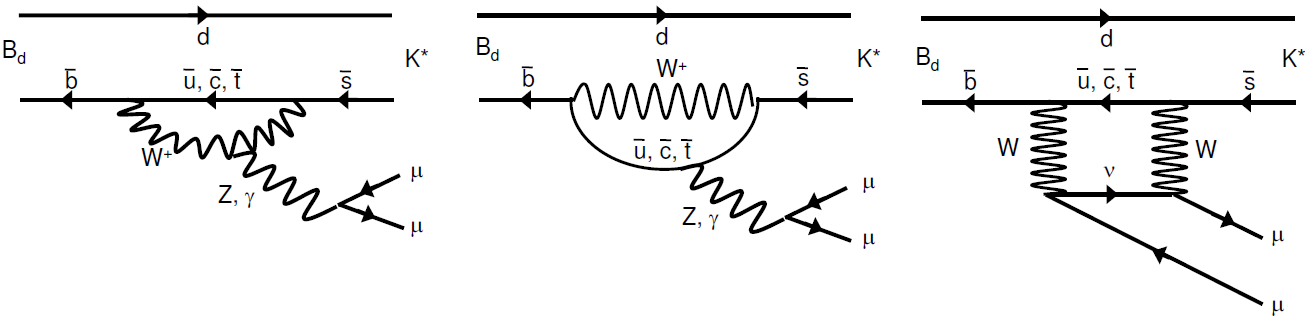
\includegraphics[width=0.66\columnwidth]{chapter2/figs/Feyn.png}
\caption[Feynman diagrams for a b to s transition]
{Three different Feynman diagrams showing the SM process that allow a \bsll transition,
 two penguin diagrams and a \W box diagram. ~\label{fig:bssm}}
\end{figure}
Processes which contain a \bquark\to\squark transition are popular FCNC decays for tests of contributions from new physics~\cite{Melikhov:1998cd}.
Measurements of FCNCs are model-independent tests of any new physics model that contribute to change the overall properties of the decay.

The formalism of \bquark-hadron decays can be expressed in terms of an effective theory, which separates different contributions to the decay 
by a particular mass scale. 
The effective theory of \B decays, Heavy Quark Effective Theory~\cite{Mannel:2004ce,Manohar:2000dt} ,
separates out particles with masses much greater than that of a \bquark quark, 
such as the electroweak gauge bosons, the Higgs, the \tquark quark and any new massive particles.
The operator product expansion separates these high and low energy contributions into a set of coefficients and operators~\cite{Wilson:1972ee},
\begin{align}
\bra{f}\mathcal{H}\ket{i} &=  \sum_k \C{k}(\mu) \bra{f}\Ope{k} (\mu)\ket{i}  \, ,
\end{align}
where the Wilson coefficients ($C$) and the operators ($O$) are normalised to a mass scale ($\mu$).

The operators encode the low energy contributions from the quarks in the decay and the Wilson coefficients encode
 the contributions from higher mass particles above the mass scale $\mu$.
For this reason the Wilson coefficients are said to encode the `short' distance physics whilst the 
operators encode the `long' distance physics.
The short distance physics covers everything above the mass scale of the effective Hamiltonian, 
such weak interactions and any contribution from physics beyond the SM.
The long distance physics covers everything below the mass scale of the Hamiltonian, 
\ie~the \Kstar physics and the interactions with the light spectator quark.
The benefit of this formalism is that the Wilson coefficients can include arbitrary contributions from new physical models and 
provide a model-independent formalism through which to measure these contributions.

The effective Hamiltonian for the \bsll transition~\cite{AltmannshoferBall} is
\begin{align}
H = \frac{4G_F}{\sqrt{2}} V_{tb}^{*} V_{ts} \sum_{i=1}^{10} C_i(\mu) O_i(\mu) \, .
\end{align}
The electroweak penguin operators are 
\begin{subequations}\begin{align}
\Ope{7}  &= \frac{e}{g^2}  m_b\left(\bar{\squark}\sigma_{\mu\nu}\frac{1}{2}(1\pm\gamma^5)\bquark\right) F^{\mu\nu}   \, , \\
\Ope{8}  &= \frac{1}{g} m_b\left(\bar{\squark}\sigma_{\mu\nu}T^a\frac{1}{2}(1\pm\gamma^5)\bquark\right) G^{a,\mu\nu}   \, , \\
\Ope{9}  &= \frac{e^2}{g^2} m_b\left(\bar{\squark}\gamma_\mu\frac{1}{2}(1\mp\gamma^5)\bquark\right) (\bar{\ell} \gamma^\mu \ell ) \, , \\
\Ope{10}  &= \frac{e^2}{g^2} m_b\left(\bar{\squark}\gamma_\mu\frac{1}{2}(1\mp\gamma^5)\bquark\right) (\bar{\ell} \gamma^\mu \gamma^5 \ell ) \, ,
\end{align}\end{subequations}
where $g$ is the strong coupling constant and $m_b$ is the \bquark mass dependent on the chosen renormalisation scheme.
The operator \Ope7  describes the electroweak penguin decay with a photon propagator, \Ope8 describes the diagram with a gluon propagator 
and the operators \Ope9 and \Ope10 describe the diagrams with electroweak bosons, either \Wpm or \Z.
The respective Wilson coefficients for these quark transitions are \C7 , \C8 , \C9 and \C{10} ~\cite{Bobeth:1999mk}.
The Wilson coefficients at the \bquark mass are evolved down from the weak mass scale, giving effective Wilson coefficients which also
include contributions from the four-quark and gluonic operators \C{1\to6},
\begin{align}
\Ceff7 &= \frac{4\pi}{\alpha_S} \C7 - \frac{1}{3} \C3 - \frac{4}{9} \C4 - \frac{20}{3} \C5 - \frac{80}{9} \C6 , \\
\Ceff8 &= \frac{4\pi}{\alpha_S} \C8 + \C3 - \frac{1}{6} \C4 + 20 \C5 - \frac{10}{3} \C6 , \\
\Ceff9 &= \frac{4\pi}{\alpha_S} \C9 + Y(\qsq) \\
\Ceff10 &= \frac{4\pi}{\alpha_S}\C{10} \\
\Ceff_{7,8,9,10} &= \frac{4\pi}{\alpha_S}\Cpeff{7,8,9,10} \, .
\end{align}
where Y(\qsq), along with more detail about the effective coefficients can be found in Ref~\cite{AltmannshoferBall}.
Contributions from physics beyond the SM can also be parameterised in terms of the Wilson coefficients.
Right handed currents for each operator can be introduced as primed counterparts to the SM Wilson coefficients (\Cp{7}, \Cp{8}, \Cp{9} and \Cp{10} ) and 
 contributions from new scalars and pseudoscalar particles can be incorporated in the form of additional Wilson coefficients \C{S} and \C{P} .

Constraints on the Wilson coefficients can be obtained from measurements of different FCNCs~\cite{Altmannshofer:2012az}.
Measurements of \btosgam transitions are proportional to the magnitude of \C{7} and measurements of 
\bsll transitions in the form of \Bsmm are proportional the value of \C10 and could incorporate contributions from \C{S} and \C{P} .
The \bsll electroweak penguin decay is mainly parameterised by \C{7}, \C9 and \C{10} , allowing 
 measurements of the \bsll decays to constrain a wide range of models of physics beyond the SM.

%Theoretical predictions for each of the Wilson coefficients come from several methods depending on the energy given to 
%the \ellell and \kpi pair.
%For the energy region where the \Kstarz meson carries a large proportion of the available energy,
% the `large recoil' region, a technique called QCD factorisation can be used~\cite{Beneke:2000wa}.
% \emph{ QCD factorisation does something I still don't understand }
%There are two other regions, the dimuon range close to the charmonium (\jpsi and \psitwos) resonances 
% and the limit of soft \Kstarz and high momentum dimuon where two different approaches must be taken, as described in 
% Refs~\cite{Khodjamirian:2010vf} and~\cite{Bobeth:2011nj} respectively.




\section{Experimental results}

The first measurement of a \bquark\to\squark FCNC was the \btosgam transition observed in the measurement of the branching fraction of \decay{\B}{\Kstar\g} at \cleo in 1993~\cite{PhysRevLett.71.674}.
\BdKstGam is a radiative electroweak penguin decay described by the photon operator \Ope7 and hence is sensitive to \C7 .
Subsequent precision measurements of \BdKstGam and 
the similar decay \BsPhiGam have been performed by the B factories, \babar~\cite{babar:exp-b2kstgamma:2009} 
and \belle~\cite{PhysRevLett.103.241801} along with \lhcb~\cite{LHCb-PAPER-2011-042,LHCb-PAPER-2012-019,LHCb-CONF-2012-004}.
These measurements of the differential branching fraction of \BdKstGam, \BsPhiGam and measurements of 
the \CP asymmetry \ACP(\BdKstGam)~\cite{PDG2012} agree well with the predictions from the SM~\cite{hfag:2012,Ali:th-b2vgamma-NNLO:2008}.

The FCNC decay \BdToKstll was proposed as a further test for contribution from physics beyond the SM in Ref~\cite{PhysRevD.61.114028}.
However, the differential branching fraction of the inclusive decay \BdToKstll and the exclusive decay \BdToKstmm 
have been measured~\cite{hfag:2012} to be
\begin{align}
\Gamma(\BdToKstll) &= 9.9^{+1.2}_{-1.1} \times 10^{-7} \\
\Gamma(\BdToKstmm) &= 1.06\pm0.10 \times 10^{-6}
\end{align}
and are compatible with SM prediction~\cite{Ligeti:2007sn,Huber:2007vv}.

Further measurements of \BdToKstll are based on  evaluating the
angular distribution of the daughter particles to understand the \Kstarz polarisation amplitudes.
How to determine the maximal amount of information from the decay
while keeping uncertainties from QCD minimal has recently attracted much 
interest~\cite{Kruger:2005ep,Egede:2008uy,AltmannshoferBall,Egede:2010zc,Bobeth:2010wg,Matias:2012xw}.

The results from the experimental analyses of 
\BdToKstll~\cite{Aubert:2008ju,PhysRevLett.103.171801,Aaltonen:2011cn,Aaij:2011aa} 
have focused on the forward-backward asymmetry of the
dimuon system (\AFB) and the fraction of longitudinal polarisation of
the \Kstarz (\FL) as a function of the dimuon invariant mass.
The latest measurements from \babar, \belle and \cdf for \FL and \AFB are shown in Fig.~\ref{fig:otherexp}.
\begin{figure}[tbp]
\centering
\subfigure[\FL]{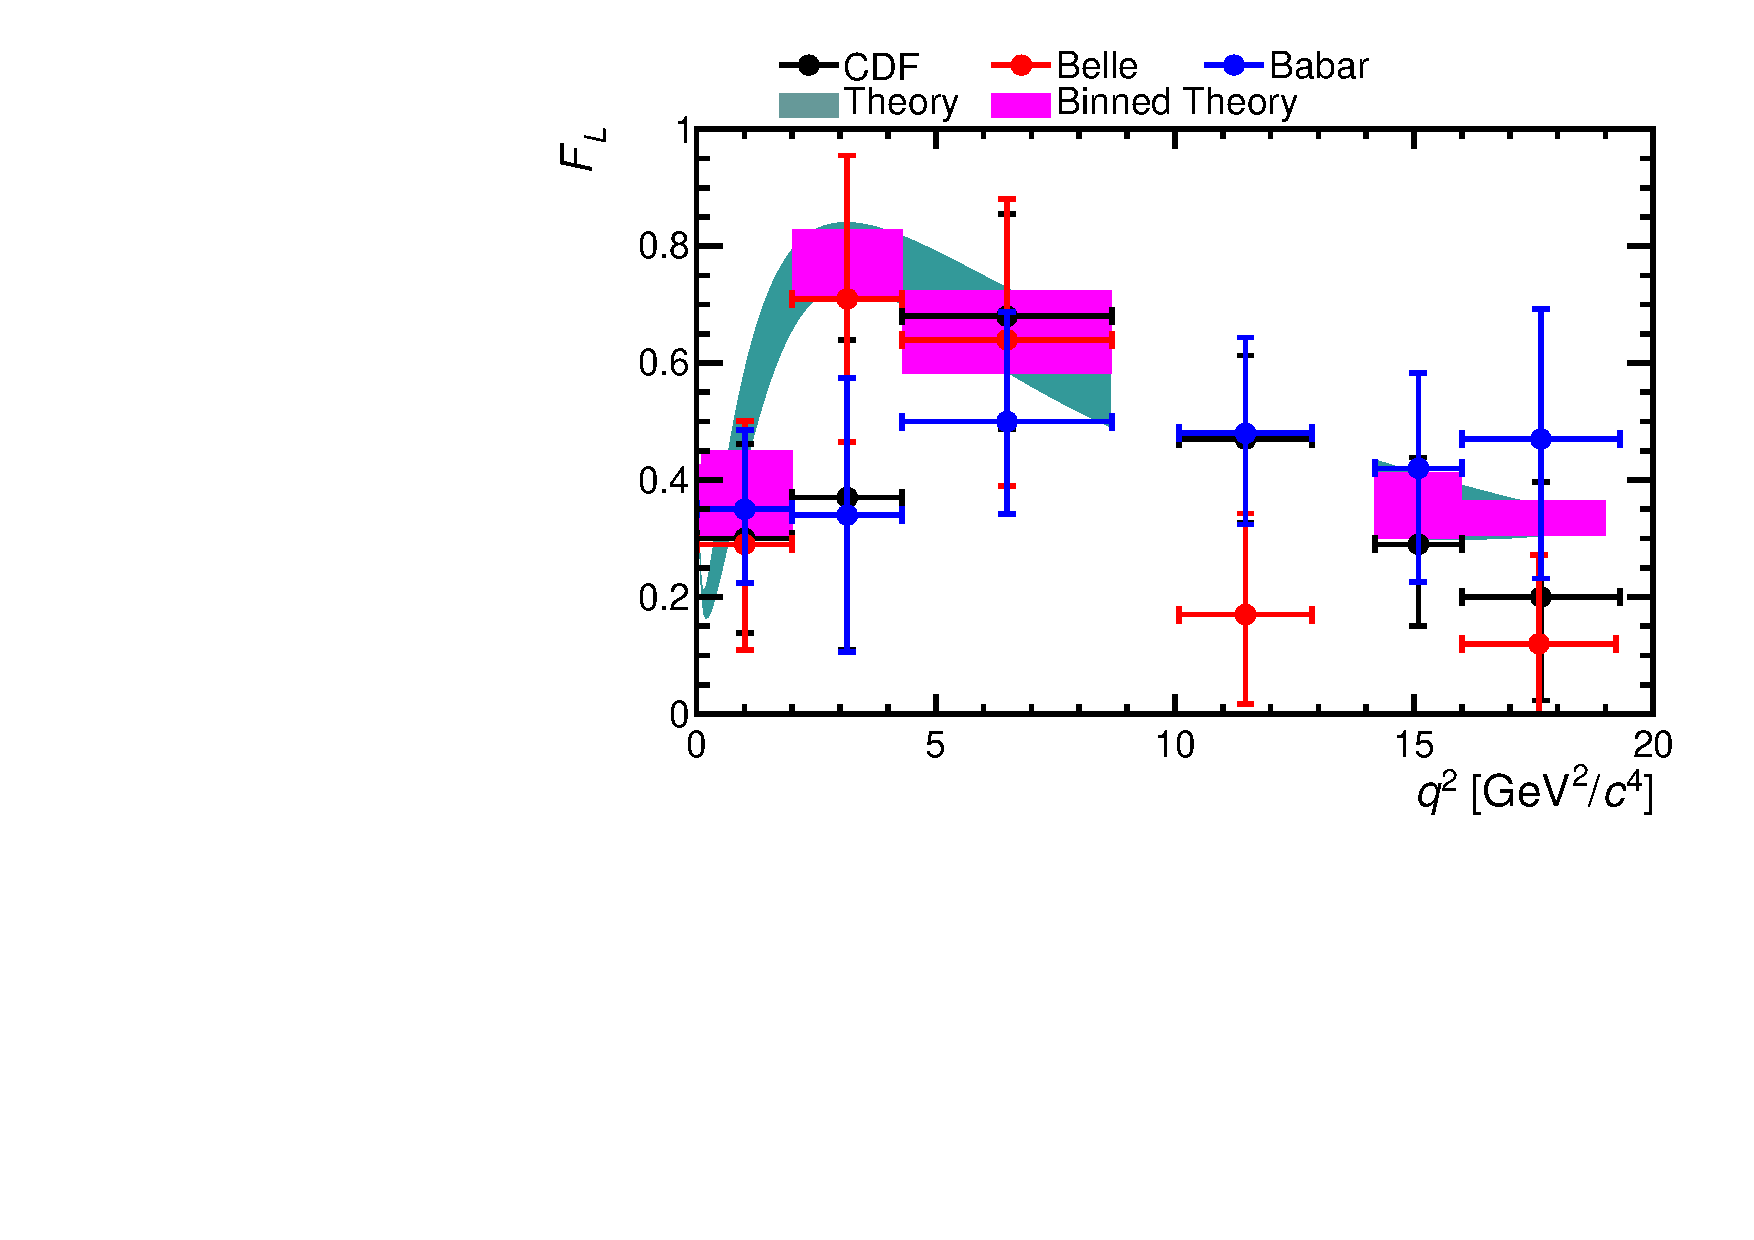
\includegraphics[width=0.48\columnwidth]{chapter2/figs/plot_FLExp.pdf}}
\subfigure[\AFB]{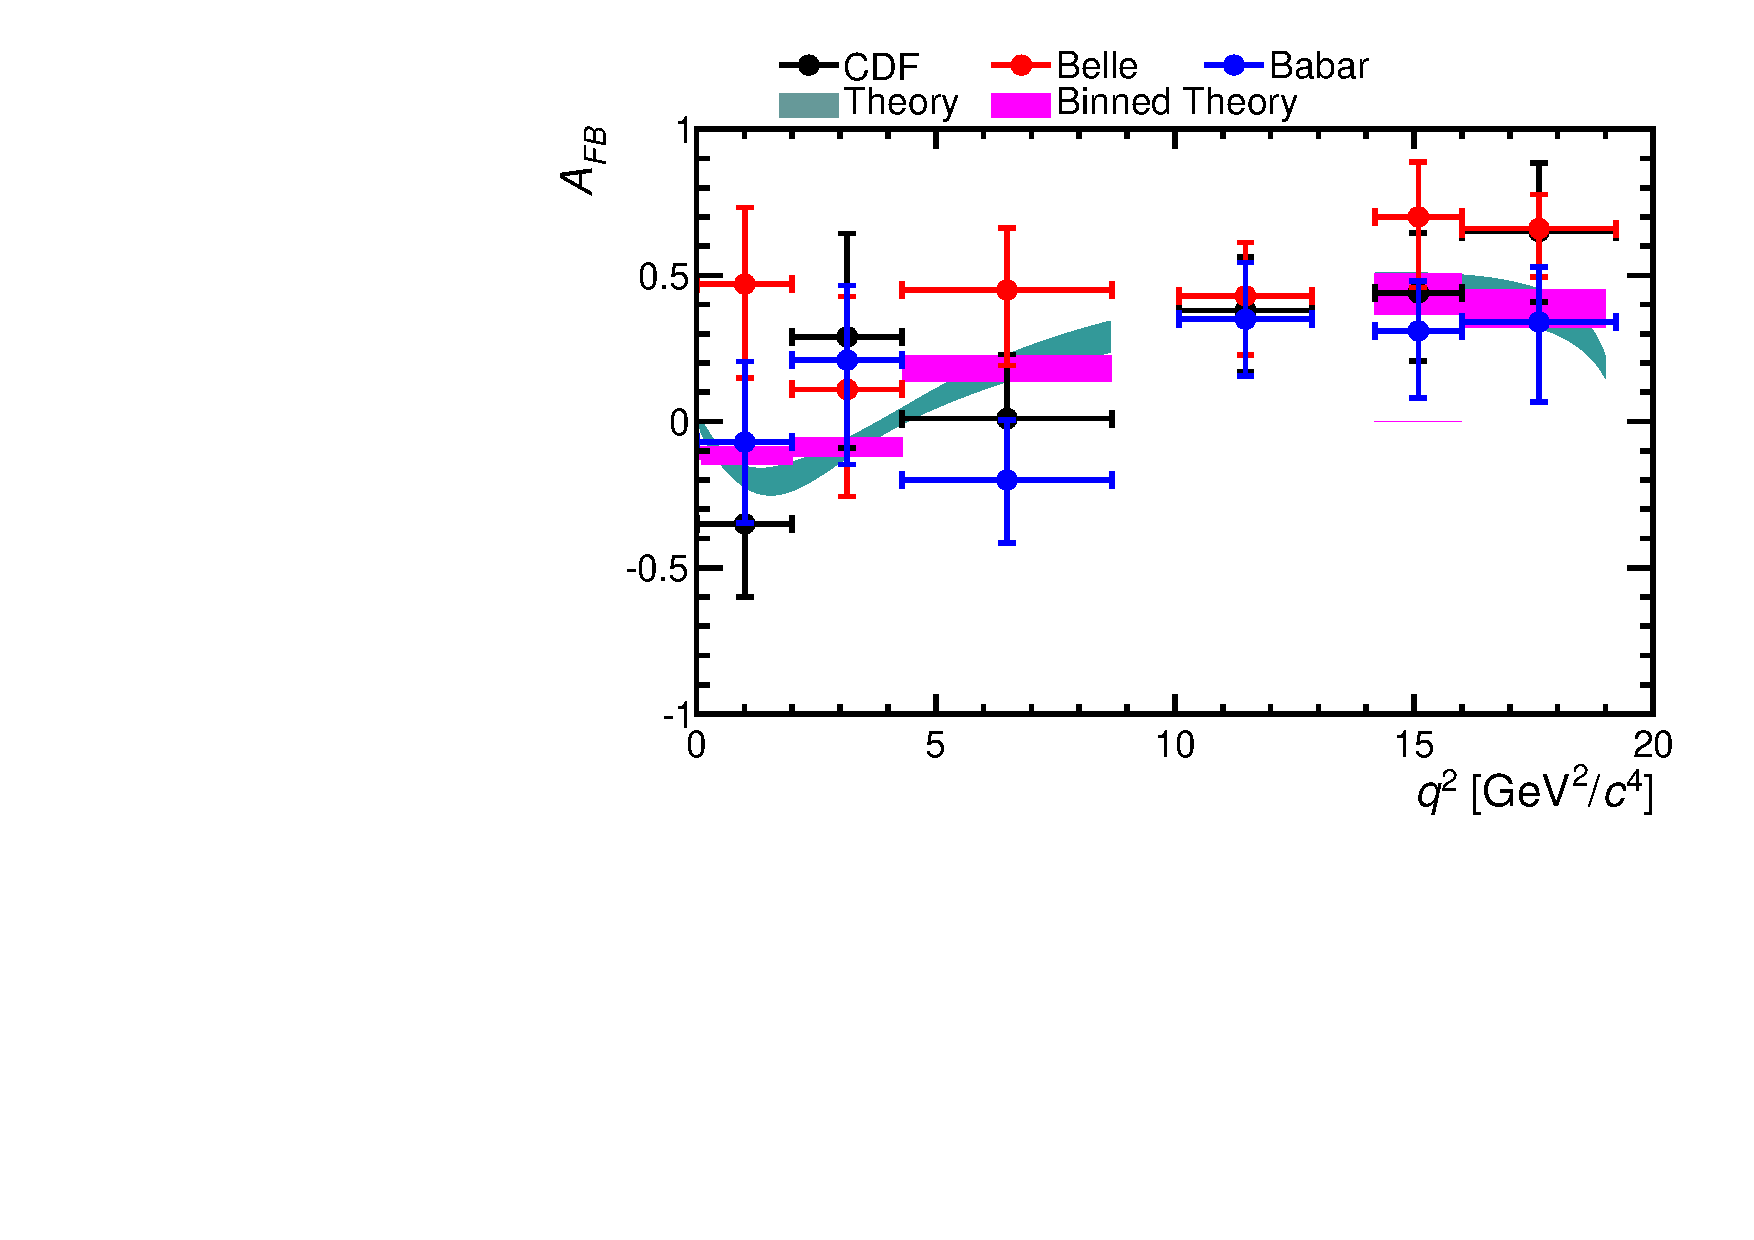
\includegraphics[width=0.48\columnwidth]{chapter2/figs/plot_AFBExp.pdf}}
\caption[\BdToKstmm measurements from \babar, \belle and \cdf]
{The fraction of longitudinal polarisation of the \Kstarz (\FL) and 
the  forward-backward asymmetry of the dimuon system (\AFB)  as measured by
\cdf~\cite{Aaltonen:2011cn,Aaltonen:2011ja}, \belle~\cite{PhysRevLett.103.171801} 
and \babar~\cite{Aubert:2007hz,Aubert:2008ju} 
along with the theoretical prediction from Ref.~\cite{Bobeth:2011gi}.~\label{fig:otherexp} }
\end{figure}
It is possible to see that there is some tension between these measurements of both \FL and \AFB at low dimuon invariant masses.
Contributions from physics beyond the SM have been predicted to change the \qsq spectrum of  \AFB~\cite{Egede:2010zc} which are not excluded by these measurements.
New measurements of \FL and \AFB are  needed to understand the exact shape of \AFB and clarify the discrepancy in the regions of low and high \qsq.
%In this thesis, the world-best measurements of the angular observables of \BdToKstmm using data from the \lhcb experiment presented along with 
%new measurements of the \kpi system.% do help understanding of the result of current and future angular analyses.


\doublepage
\chapter{The \BdToKstll decay	}
\label{chap:kstmm:theo}

\section{Angular basis}
\label{sec:kstmm:basis}

The differential angular distribution for \BdToKstll is expressed as a
function of  five kinematic variables: three angles (\ctl, \ctk, $\phi$) 
and two invariant masses;
the mass squared of the \kpi system is denoted \psq and the 
mass squared of the dilepton pair (\qsq),  
the angle $\theta_K$ is defined as the angle between the \Kp and the \B momentum
vector in the rest frame of the \Bd.  The angle $\theta_\ell$ is
 defined as the one between the \ellp in the rest frame of the dilepton
pair and the momentum vector of the \Bd.  The angle $\phi$ is defined
as the signed angle between the planes formed by the dilepton pair and the \kpi pair respectively, 
in the rest frame of the \Bd.\footnote{This is the same sign convention for \ctl as used in all 
previous experiments and the same $\phi$ convention as used in 
\lhcb~\cite{Aaij:2013iag}.}

For the \CP-conjugate decay \BdbToKstbll, $\theta_\ell$ is defined with respect to the \ellm instead of the \ellp
and $\theta_K$ is defined with respect to the \Km instead of the \Kp.
There are two possible definitions of $\phi$, a \CP symmetric definition which 
changes through a minus sign and a \CP anti-symmetric definition, \phiacp, 
which is unchanged between the \Bd and \Bdb decay. 
An illustration of the angles for \BdbToKstbll is shown in Fig~\ref{fig:kstmm:angles}.
\begin{figure}[tbp]
\centering
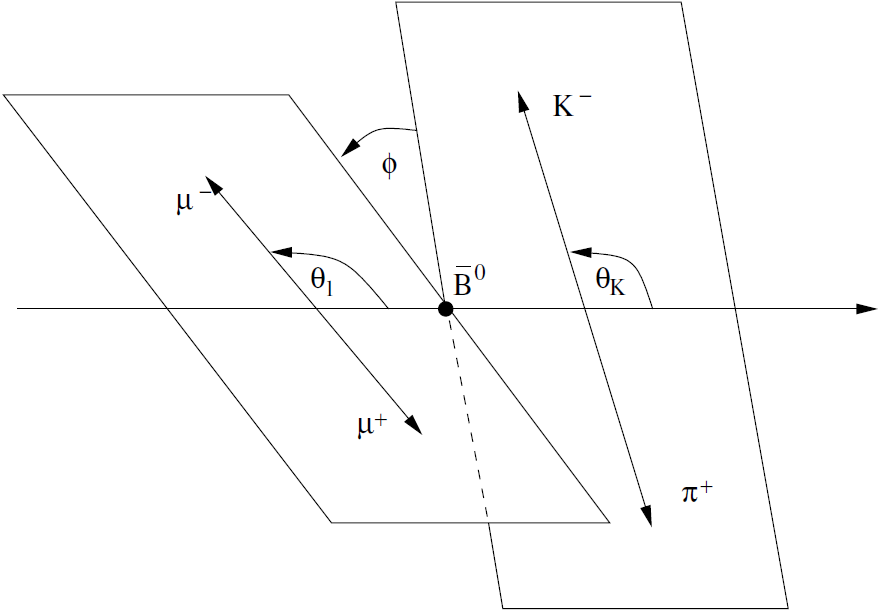
\includegraphics[width=0.48\columnwidth]{chapter4/figs/restMassAngles.png}
\caption[An illustration of the angles used to describe the \BdbToKstbll decay.]
{An illustration of the angles used to describe the \BdbToKstbll decay.
 The angle $\theta_l$ is defined between the \ellm and the \Bdb in the dilepton rest frame.
 The angle $\theta_K$ is defined between the \Km and the \Bdb in the \kpi rest frame.
 The angle $\phi$ is the signed angle between $\ellm$ and $\Km$ in the rest frame of the \Bdb. 
~\label{fig:kstmm:angles} }
\end{figure}

The angles \ctl and \ctk are given explicitly as 
\begin{align}
\ctl = \left( \frac{ \vec{p}_{\ellp} \cdot \vec{p}_{\ellell}  }{|\vec{p}_{\ellp}||\vec{p}_{\ellell}|} \right), \quad 
\ctk = \left( \frac{ \vec{p}_{\Kp} \cdot \vec{p}_{\kpi}  }{|\vec{p}_{\Kp}||\vec{p}_{\kpi}|}  \right) \, ,
\end{align}
where each momentum vector $\vec{p}$ is defined in the rest frame of the parent particle, i.e. 
the lepton momentum, $\vec{p}_{\ellp}$, is in the dilepton rest frame and dilepton momentum, $\vec{p}_{\ellell}$, is in \Bd rest frame.
The angle $\phi$ is calculated as %the difference between the angles $\theta_\ell$ and $\theta_K$ and
\begin{align}
\cos\phi &=    \left( \frac{\vec{p}_{\ellp} \times \vec{p}_{\ellm} }{|\vec{p}_{\ellp} \times \vec{p}_{\ellm}|} \right) \cdot 
   \left( \frac{\vec{p}_{\Kp} \times \vec{p}_{\pim} }{|\vec{p}_{\Kp} \times \vec{p}_{\pim}|} \right)  \, .
\end{align}
%and
%\begin{align}
%\sin\phi =    \left(\frac{ \vec{p}_{\ellp} \times \vec{p}_{\ellm} }{|\vec{p}_{\ellp} \times \vec{p}_{\ellm}|} \right) \times 
%   \left(\frac{ \vec{p}_{\Kp} \times \vec{p}_{\pim} }{|\vec{p}_{\Kp} \times \vec{p}_{\pim}|} \right) 
%   \cdot \frac{\vec{p}_{\kpi}}{|\vec{p}_{\kpi}|}  \, .
%\end{align}
For the CP-conjugate \BdbToKstbll decay, the angles \ctl and \ctk are given explicitly as 
\begin{align}
\cos\theta_{\bar{\ell}} &= \left( \frac{ \vec{p}_{\ellm} \cdot \vec{p}_{\ellell}  }{|\vec{p}_{\ellm}||\vec{p}_{\ellell}|} \right), \quad 
\cos\theta_{\bar{K}} = \left( \frac{ \vec{p}_{\Km} \cdot \vec{p}_{\kpi}  }{|\vec{p}_{\Km}||\vec{p}_{\kpi}|}  \right) \, ,
\end{align}
and applying the \CP operator to the definition of $\phi$ gives the relation,
\begin{align}
\cos\phi &= \left( \frac{\vec{p}_{\ellm} \times \vec{p}_{\ellp} }{|\vec{p}_{\ellm} \times \vec{p}_{\ellp}|} \right) \cdot 
   \left( \frac{\vec{p}_{\Km} \times \vec{p}_{\pip} }{|\vec{p}_{\Km} \times \vec{p}_{\pip}|} \right)  \, . 
\end{align}
The \CP anti-symmetric definition of $\phi$ is given by only applying the \CP operator to the \kpi state, 
\begin{align}
\cos\phiacp &= \left( \frac{\vec{p}_{\ellp} \times \vec{p}_{\ellm} }{|\vec{p}_{\ellp} \times \vec{p}_{\ellm}|} \right) \cdot 
   \left( \frac{\vec{p}_{\Km} \times \vec{p}_{\pip} }{|\vec{p}_{\Km} \times \vec{p}_{\pip}|} \right)  \, .
\end{align}

Each of the angles are defined over the intervals
\begin{align}
0 \leq \theta_{\textit{l}} < \pi, \quad 0 \leq \theta_{\textit{K}} < \pi, \quad -\pi \leq \phi < \pi,
\end{align}
such that the angular distribution is defined over the range
\begin{align}
-1 \leq \ctl < 1, \quad -1 \leq \ctk < 1, \quad -\pi < \phi < \pi \, .
\end{align}

%section
\section{Angular distribution}
\label{sec:fullangdist}

Following Ref~\cite{PhysRevD.61.114028}, the angular distribution of \BdToKstll can be written as an explicit function
of \ctl and $\phi$, 
\begin{align}
\frac{\text{d}^5\Gamma}{\text{d}q^2 \text{d}p^2 \text{d}\ctk \text{d}\ctl \text{d}\phi} = & 
\frac{3}{8} \left( I_1^c + 2I_1^s + (I_2^c + 2I_2^s) \cos2\theta_l  + 2I_3\stlsq\cos2\phi \right. \nonumber \\
&+ 2\sqrt{2}I_4\sin2\theta_l\cos\phi  + 2\sqrt{2}I_5\stl\cos\phi + 2I_6\ctl \nonumber\\ 
&+ \left. 2\sqrt{2}I_7\stl\sin\phi  + 2\sqrt{2}I_8\sin2\theta_l\sin\phi + 2\sqrt{2}I_9\stlsq\sin2\phi \frac{}{} \right) \, ,
\end{align}
where each of the angular coefficients ($I_i$) are combinations of the helicity amplitudes and contain
 an implicit dependence on \ctk and the invariant masses, \psq and \qsq.

The nine angular coefficients are expressed as
\begin{subequations}\begin{align}
I_1^c &= |\mathcal{A}_{0L}|^2 + |\mathcal{A}_{0R}|^2 + 8\frac{m_l^2}{q^2}\Re(\mathcal{A}_{L0}\mathcal{A}_{R0}^{*}) + 4\frac{m_l^2}{q^2}|\mathcal{A}_t|^2 \frac{}{}   \\
I_1^s &= \frac{3}{4} ( |\mathcal{A}_{L||}|^2 + |\mathcal{A}_{L\bot}|^2 + (L\to R) )  ( 1 - \frac{4m_l^2}{q^2} ) +  \frac{4m_l^2}{q^2}\Re( \mathcal{A}_{L\bot} \mathcal{A}_{R\bot}  + \mathcal{A}_{R||} \mathcal{A}_{R||} ) )  \frac{}{} \\
I_2^c &= - \beta_l^2 \left( |\mathcal{A}_{L0}|^2 + |\mathcal{A}_{R0}|^2 \right) \frac{}{} \\
I_2^s &= \frac{1}{4} \beta_l^2 \left( |\mathcal{A}_{L||}|^2 + |\mathcal{A}_{L\bot}|^2 + |\mathcal{A}_{R||}|^2 + |\mathcal{A}_{R\bot}|^2  \right)  \frac{}{} \\
I_3 &= \frac{1}{2} \beta_l^2  \left( |\mathcal{A}_{1L\bot}|^2 - |\mathcal{A}_{1L||}|^2 + |\mathcal{A}_{R\bot}|^2 - |\mathcal{A}_{R||}|^2 \right) \frac{}{}  \\
I_4 &= \frac{1}{\sqrt{2}}   \beta_l^2  \left(  \Re(\mathcal{A}_{L0}\mathcal{A}_{L||}^{*}) + (L\to R) \right) \frac{}{} \\
I_5 &= \sqrt{2}  \beta_l \left(  \Re(\mathcal{A}_{L0}\mathcal{A}_{L\bot}^{*}) - (L\to R) \right) \frac{}{} \\
I_6 &= 2   \beta_l \left( \Re(\mathcal{A}_{L||}\mathcal{A}_{L\bot}^{*}) - (L\to R) \right) \frac{}{} \\
I_7 &= \sqrt{2}  \beta_l \left(  \Im(\mathcal{A}_{L0}\mathcal{A}_{L||}^{*}) - (L\to R) \right) \frac{}{} \\
I_8 &= \frac{1}{\sqrt{2}}  \beta_l^2 \left(  \Im(\mathcal{A}_{L0}\mathcal{A}_{L\bot}^{*}) + (L\to R) \right) \frac{}{} \\
I_9 &=  \beta_l^2 \left(  \Im(\mathcal{A}_{L||}\mathcal{A}_{L\bot}^{*}) + (L\to R) \right) , \frac{}{}
\end{align}\end{subequations}
where $\mathcal{A}_{H(0,||,\bot,t)}$ are the \Kstarz spin amplitudes for a given handedness, $m_l$ is the lepton mass
 and $\beta_l = \sqrt{ 1 - 4m_l^2/\qsq}$~\cite{PhysRevD.61.114028}. 
The lepton mass is assumed to be insignificant, such that $I_{1,2}$ have no $m_l$
dependence, $\beta_l=1$ and $\mathcal{A}_t$ disappears from the angular distribution.

Neglecting any \CP asymmetry, as measured in Ref.~\cite{LHCb-PAPER-2012-021},
%and using $\phi = \phi_{sym}$, 
the \Bd and \Bdb decays can be combined to give 
\begin{align}
\frac{\text{d}^5\left[\Gamma_{\Bd} + \Gamma_{\Bdb} \right] }{\text{d}q^2 \text{d}p^2 \text{d}\ctk \text{d}\ctl \text{d}\phi} = \sum_{i=1}^{9} I_i (\ctl,\ctk,\phi) + \bar{I}_i (\ctl,\ctk,\phi) \ .
\end{align}
The \CP anti-symmetric angular distribution is given by 
\begin{align}
\frac{\text{d}^5\left[\Gamma_{\Bd} - \Gamma_{\Bdb} \right] }{\text{d}q^2 \text{d}p^2 \text{d}\ctk \text{d}\ctl \text{d}\phi} = \sum_{i=1}^{9} I_i (\ctl,\ctk,\phi) - \bar{I}_i (\ctl,\ctk,\phiacp) \ .
\end{align}
Simplification of the angular distribution can be achieved by applying a transformation 
 in $\phi$ such that $\phiprime = \phi - \pi $ 
for $\phi < 0 $~\cite{Ksteepubnote}.
The $I_{4,5,7,8}$ angular terms which are dependent on $\cos\phi$ or
$\sin\phi$ cancel, leaving $I_{1,2,3,6,9}$ in the angular distribution.

For a \kpi state which is a combination of different resonances,
the amplitudes for a given handedness ($H=L,R$) can be expressed as a
sum over the resonances ($J$)~\cite{Lu:2011jm},
\begin{equation}
\label{eq:amp}
\begin{aligned}
\mathcal{A}_{H,0/t}^{L,R}(\psq,\qsq) &= \sum_J \sqrt{N_J} \ A_{J,H,0}^{L,R}(\qsq) \ P_J(p^2) \ Y_J^0 (\theta_K,0)  \\
\mathcal{A}_{H,||/\bot}^{L,R}(\psq,\qsq) &= \sum_J \sqrt{N_J} \ A_{J,H,||/\bot}^{L,R}(\qsq) \ P_J(p^2) \ Y_J^{-1} (\theta_K,0) , 
\end{aligned}
\end{equation}
where $Y_J^m (\theta_K, 0)$ are the spherical harmonics, $\mathcal{M}$
is the matrix element encompassing the \qsq dependence
 and $P_J(\psq)$ is the propagator of the resonant \Kstarz state.




%section
\section{Amplitudes}
\label{sec:kstmm:amps}

The amplitudes of \BdToKpill parametrise the decay and are different for each polarisation of the \kpi state and of the dilepton system.
The dilepton is a vector state and the \kpi system is considered to be in a scalar (S-wave) or a vector (P-wave) state.
The matrix element for  \BdToKpill takes the same form for  both \kpi states and can be written~\cite{AltmannshoferBall} as
\begin{align}
\mathcal{M} =& \frac{G_F \alpha_s}{2\pi} \Vtb\Vts \bigg( \bigg[ \bra\kpi  \bar{s}\gamma_\mu \left( \Ceff9 P_L + \Cpeff9 P_R \right) \bquark \ket{\bar{B}}  \nonumber \\
 &  - \frac{2m_b}{\qsq} \bra\kpi  \bar{s} i \sigma^{\mu\nu} q_\nu \left( \Ceff7 P_R + \Cpeff7 P_L \right) \bquark\ket{\bar{B}} \bigg] \left( \bar{\ell}\gamma_{\mu} \ell\right)  \nonumber \\
 &  + \bra\kpi  \bar{s} \gamma^\mu \left( \Ceff10 P_L + \Cpeff10 P_R \right) b \ket{\bar{B}} \left( \bar{\ell} \gamma_\mu \gamma_5 \ell \right)   \bigg)    
\end{align}
where contributions from scalar and pseudoscalar operators have been ignored.

\subsection{\BdToKstll}

The \kpi P-wave has three polarisation states:
The total amplitude for the decay of a pseudo-scalar to two vector particles, $\decay{P}{V_1 V_2}$, can be written as a combination of the 
polarisation tensors and the matrix element,
\begin{align}
\label{eq:pol}
M(\decay{P}{V_1 V_2}) &= \epsilon_{V_1}^{*\mu} M_{\mu\nu} \epsilon_{V_2}^{*\nu} \, .
\end{align}
Each of the polarisation states for a vector state described by the momentum vector 
$p^\mu = \left(p_0, 0, 0, p_z\right)$ can be written as
\begin{subequations}\begin{align}
\epsilon_V^\mu(\pm) &= \left( 0, 1, \pm i, 0\right) / \sqrt{2} \\
\epsilon_V^\mu(0) &= \left( p_z, 0, 0, -p_0\right) / \sqrt{p^2} \\
\epsilon_V^\mu(t) &= \left( p_0, 0, 0, p_z\right) / \sqrt{p^2} \ .
\end{align}\end{subequations}
In the context of the decay \BdToKstll there is a virtual gauge boson and a real \Kstarz.
The gauge boson can exist in all four possible polarisation states $(0, \pm, t)$ but the \Kstarz is on shell and only 
 has three states $(0, \pm)$.
The helicity amplitudes can be obtained by contracting the polarisation states for each of the 
particles in Eq~\ref{eq:pol} to give 
\begin{align}
H_i = M_{i,i} \, ,
\end{align}
with an implicit sum over $i = 0, ||$ and $\bot$, and additionally $H_t = M_{0,t}$.
The transversity amplitudes are combinations of the helicity amplitudes
\begin{align}
A_{||,\bot} = ( H_{+} \mp H_{-} ) \sqrt{2} , \quad A_0 = H_0 , \quad \text{and} \,  A_t = H_t 
\end{align}
The subsequent decay of the vector boson to dilepton system allows for both left and right-handed currents in 
the longitudinal, parallel and perpendicular polarisations so there are in total seven transversity amplitudes.
The transversity amplitudes  for the P-wave \Kstarzo state can be written to leading order~\cite{AltmannshoferBall} as	
\begin{subequations}\begin{align}
A_{1,L/R,0}(\qsq)=& -\frac{N}{2m_{\Kstarzo}\sqrt{\qsq}} \Bigg(  \left( (\Ceff9 - \Cpeff9 ) \mp (\Ceff10 - \Cpeff10 ) \right)  \nonumber\\ 
 & \bigg[ \left( \mB^2 - m_{\Kstarzo}^2 - \qsq \right) \left( \mB + m_{\Kstarzo} \right) A_1(\qsq) - \lambda \frac{A_2(\qsq)}{\mB + \m_{\Kstarzo}} \bigg]   \\ 
 & + 2m_b \left( \Ceff7 - \Cpeff7 \right) \bigg[ \left( \mB^2 + 3m_{\Kstarzo}^2 + \qsq \right) T_2(\qsq) - \frac{\lambda(\mB,\Kstarzo,\qsq)}{\mB^2 - m^2_{\Kstarzo}} T_3(\qsq) \bigg] \Bigg) \nonumber \\
A_{1,L/R,||}(\qsq) =& -N \sqrt{2}\left(\mB^2 - m_{\Kstarzo}^2\right) \bigg[ \left( (\Ceff9 - \Cpeff9 ) \mp (\Ceff10 - \Cpeff10 ) \right) \frac{ A_1(\qsq) }{ \mB + m_{\Kstarzo} } \nonumber \\
& + 2\frac{m_b}{\qsq} \left( \Ceff7 - \Cpeff7 \right) T_ 2(\qsq) \bigg] \\
A_{1,L/R,\bot}(\qsq) =&  N \sqrt{2} \lambda(\mB,\Kstarzo,\qsq)^{1/2}  \bigg[ \left( (\Ceff9 - \Cpeff9 ) \mp (\Ceff10 - \Cpeff10 ) \right) \frac{ V(\qsq) }{ \mB + m_{\Kstarzo} } \nonumber \\
& + 2\frac{m_b}{\qsq} \left( \Ceff7 + \Cpeff7 \right) T_1(\qsq) \bigg] 
\end{align}\end{subequations}
with $\lambda(\mB,\psq,\qsq) = \left( \mB^2 - \psq - \qsq \right)^2 - 4\psq\qsq$.
This expression uses the narrow width assumption for the \Kstarz(892) which assumes the \Kstarz decays on shell to \kpi, 
 allowing the relativistic Breit-Wigner to be approximated as
\begin{align}
P_1^2(\psq) = \frac{1}{\left(\psq + m_{\Kstarz}^2\right)^2 +m_{\Kstarz}^2 \Gamma_{m_{\Kstarz}}^2 }   \frac{m_{\Kstarz}\Gamma_{m_{\Kstarz}}}{\pi}  \quad \to   \quad  \delta\left(\psq-m_{\Kstarz}^2\right) \ .
\end{align}
The transversity amplitudes can then be expressed in terms of seven \B\to\Kstarzo form factors ($A_i(\qsq), T_i(\qsq), V(\qsq)$).
For large \Kstar energies, of order $\mB/2$, it is possible to reduce the seven different 
form factors to two \emph{heavy-to-light} form factors as in Ref~\cite{Kruger:2005ep}.
This allows the amplitudes to take a simple form neglecting corrections of order $1/m_b$ and $\alpha_S$,
\begin{subequations}\begin{align}
A_{1,L/R,0}(\qsq)=& -\frac{N}{2m_{\Kstarzo}\sqrt{\qsq}} (1-\qsq)^2 \Bigg[  \left( (\Ceff9 - \Cpeff9 ) \mp (\Ceff10 - \Cpeff10 ) \right) \nonumber\\
&+ 2m_b \left( \Ceff7 - \Cpeff7 \right) \Bigg]  \xi_{||}\left(E_{\Kstarz}\right)   \\
A_{1,L/R,||}(\qsq) =& -N \sqrt{2}\mB (1-\qsq) \bigg[ \left( (\Ceff9 - \Cpeff9 ) \mp (\Ceff10 - \Cpeff10 ) \right) \nonumber\\ 
& + 2\frac{m_b}{\qsq} \left( \Ceff7 - \Cpeff7 \right) \bigg] \xi_{\bot}\left(E_{\Kstarz}\right) \\
A_{1,L/R,\bot}(\qsq) =& + N \sqrt{2}  \mB (1-\qsq) \bigg[ \left( (\Ceff9 - \Cpeff9 ) \mp (\Ceff10 - \Cpeff10 ) \right) \nonumber \\
& + 2\frac{m_b}{\qsq} \left( \Ceff7 + \Cpeff7 \right)  \bigg] \xi_{\bot}\left(E_{\Kstarz}\right) \, .
\end{align}\end{subequations}

\subsection{\BdToKpill amplitudes}

Non-resonant \kpi effects in have been explored in Ref~\cite{Grinstein:2005ud} and the combination of multiple
 \Kstar resonances have been explored in Ref~\cite{Lu:2011jm}.
A combination of several resonant \kpi states can be achieved though the dependence
of the matrix elements on the resonant mass, $m_{\Kstarzj}$ 
and adding coefficients derived from the polarisation tensor~\cite{Lu:2011jm}.
The effect of a \kpi S-wave has been explored in Refs~\cite{Becirevic:2012dp,Matias:2012qz} and also in more detail later in Chapter~\ref{chap:swave:theo}.
The single \Kstarzz S-wave amplitude~\cite{Lu:2011jm} is given by
\begin{align}
A_{0,L/R,0} =& N\frac{\lambda\left(\mB,\Kstarzz\qsq\right)^{1/2}}{\sqrt{\qsq}} \bigg[ \left( (\Ceff9 - \Cpeff9 ) \mp (\Ceff10 - \Cpeff10 ) \right) F_1(\qsq)  \nonumber \\
&+ 2 m_b \left( \Ceff7 + \Cpeff7 \right) \frac{ F_T(\qsq)}{\mB + m_{\Kstarzz} }  \bigg]  
\end{align}
where $F_1(\qsq)$ and $F_T(\qsq)$ are the \Bd\to\Kstarzz form factors. 





%section
\section{Angular observables}
\label{sec:kstmm:obs}

The contributions from the Wilson coefficients defined above
 can be measured by measuring the transversity amplitudes
 through an angular analysis of the \BdToKstll angular distribution.
Direct measurements of the transversity amplitudes are dependent on the values of the form factors
 which have a significant theoretical uncertainty.
To mitigate these uncertainties and allow measurements of the Wilson coefficients, angular observables
can be constructed from the transversity amplitudes that are independent of the two heavy-to-light form factors.
Many angular observables have been proposed for the decay 
\BdToKstll~\cite{Kruger:2005ep,AltmannshoferBall,Egede:2008uy,Bobeth:2010wg,Matias:2012xw}. 
These observables are combinations of the amplitudes which both minimise the uncertainty from the form factors 
and maximise the contribution from new physics models. 
So far the forward-backward asymmetry (\AFB), the fraction of the \Kstarz longitudinal polarisation (\FL ) 
and two combinations of the transverse amplitudes (\AT2 and \AIm ) have been 
measured~\cite{Aaltonen:2011cn,Aubert:2007hz,Aaltonen:2011ja,Aubert:2008ju,PhysRevLett.103.171801}.

\subsection{P-wave observables}

These observables are constructed from combinations of amplitudes and
are normalised to the sum of amplitudes for the P-wave state, given as 
\begin{align}
|A_{10}|^2 + |A_{1||}|^2 + |A_{1\bot}|^2 \, ,
\end{align}
where the generic combination of amplitudes $A_{Ji}A_{Ji}^{*}$ is defined for a spin $J$ and a polarisation (0,$||$,$\bot$) as
\begin{align}
\label{eq:ampsq}
A_{Ji} A_{Ji}^{*} &= A_{JiL} A_{JiL}^{*} + A_{JiR} A_{JiR}^{*} \, .
\end{align}
The forward-backward asymmetry of the dilepton system, \AFB, enters in the angular coefficient $I_6$ and
is defined in terms of the amplitudes as
\begin{align}
\label{eq:theoafb}
\AFB(\qsq) &= \frac{3}{2} \frac{  \Re(A_{1L||}A_{1L\bot}^{*}) - 
\Re(A_{1R||}A_{1R\bot}^{*})}{|A_{10}|^2 + |A_{1||}|^2 + |A_{1\bot}|^2 } \, .
\end{align}
In a similar way, \FL, \OS3 and \OS9 are defined as
\begin{equation}
\begin{split}
\FL(\qsq) &= \frac{  |A_{10}|^2 } {|A_{10}|^2 + |A_{1||}|^2 + |A_{1\bot}|^2} \\
\OS3 (\qsq) &= \frac{ |A_{1\bot}|^2 - |A_{1||}|^2 }{ |A_{10}|^2 + |A_{1||}|^2 + |A_{1\bot}|^2} \\
\OS9 (\qsq) &= \frac{  \Im(A_{1L||}A_{1L\bot}^{*}) - \Im(A_{1R||}A_{1R\bot}^{*}) }{|A_{10}|^2 + |A_{1||}|^2 + |A_{1\bot}|^2} 
\end{split}
\end{equation}
where \OS3 and \OS9 are related to the angular coefficients $I_3$ and $I_9$ respectively.
These theoretical observables are normalised to the sum of the P-wave amplitudes
and the factorisation of the amplitudes into matrix elements and the 
propagators removes the \psq dependence from these theoretical observables. 

In terms of the angular distribution, \AFB can also be expressed 
as the difference 
between the number of `forward-going' \mup and the number of 
`backward-going' \mup in the rest frame of the \Bd,
\begin{align}
\label{eq:expafb}
\left[ \int_0^1 - \int_{-1}^0 \right]  \text{d}\ctl
\frac{\text{d}\Gamma}{\text{d}\qsq \text{d}\ctl} / 
\frac{\text{d}\Gamma}{\text{d}\qsq} \, ,
\end{align}
which explains the name of the observable. 

\subsection{Transverse observables}
\label{sec:kstmm:reparam}

Angular observables which are normalised to only the transverse helicity amplitudes have
 been studied with the additional aim of reducing the theoretical uncertainties~\cite{Melikhov:1998cd,Kruger:2005ep}.
This is achieved by separating out the dependence on the  longitudinal amplitudes and their form factors from the calculation.
The main transverse observable is \AT2 which comes from the angular coefficient $I_3$,
\begin{align}
\AT2 (\qsq) &=  \frac{ |A_{1\bot}|^2 - |A_{1||}|^2  }{ |A_{1\bot}|^2 + |A_{1||}|^2 }  \, .
\end{align}
The observables associated with $I_6$ and $I_9$ can be similarly reparameterised~\cite{Becirevic:2011bp} 
 to give
\begin{equation}
\begin{split}
\ATRe(\qsq) &= \frac{ |A_{1\bot}|^2 - |A_{1||}|^2 }{ |A_{1||}|^2 + |A_{1\bot}|^2} \\
\ATIm(\qsq) &= \frac{  \Im(A_{1L||}A_{1L\bot}^{*}) \Im(A_{1R||}A_{1R\bot}^{*}) }{ |A_{1||}|^2 + |A_{1\bot}|^2} \, .
\end{split}
\end{equation}
These observables are correlated to $(1-\FL)$ when the the angular distribution is normalised to the sum of the P-wave amplitudes.

\subsection{\CP asymmetric angular observables}

Angular observables equivalent to \OS3 and \OS9 for the \CP antisymmetric angular distribution can by constructed
from the definition of $I_i - \bar{I}_i$.
Two \CP antisymmetric angular observables, \OA3 and \OA9 for the angular coefficients $I_3$ and $I_9$,
which can be compared to the \OS{i} angular observables 
\begin{align}
\OA3 &= \frac{1}{2} \frac{\left(I_3 - \bar{I}_3\right)}{ |A_{10}|^2 + |A_{1||}|^2 + |A_{1\bot}|^2} \, , \\
\OA9 &= \frac{1}{2} \frac{\left(I_9 - \bar{I}_9\right)}{ |A_{10}|^2 + |A_{1||}|^2 + |A_{1\bot}|^2}  \, .
\end{align}

\subsection{Relation to the Wilson coefficients}

Each of the observables is related to the Wilson coefficients through bi-linear combinations of the transversity amplitudes.
This means that there are terms proportional to the combinations $|\Ceff{9,10} \pm \Cpeff{9,10} |^2$ and $|\Ceff7 - \Cpeff7 |^2$.
Each of these terms is multiplied by the relevant \Kstarz form factors giving the \qsq dependence. 
This can be seen in the SM predictions for \AFB and \FL in Fig.~\ref{fig:otherexp}.






%section
\section{The angular distribution with observables}
\label{sec:kstmm:angdistswithobs}

The angular distribution of \BdToKstmm including the angular observables as a function of \ctl, \ctk and \phiprime is given by
\begin{align}
\label{eq:kstmm:theo5d}
\frac{1}{\Gamma} \frac{\text{d}^4\Gamma}{\text{d}\qsq\dctk\dctl \text{d}\phiprime} & =   \frac{9}{16\pi}   \Bigg(  \xspace 2 \FL \ctksq ( 1 - \ctlsq )  \nonumber \\ 
&  \quad \quad \quad  + \frac{1}{2} ( 1 - \FL ) ( 1 - \ctksq ) ( 1 + \ctlsq )  \nonumber \\
&  \quad \quad \quad  + \frac{1}{2} ( 1 - \FL ) \AT2 ( 1 - \ctksq ) (  1 - \ctlsq ) \cos2\phiprime  \nonumber \\
&  \quad \quad \quad  +  \frac{4}{3} \AFB ( 1 - \ctksq ) \ctl  \nonumber \\ 
&  \quad \quad \quad  + \OS{3} ( 1 - \ctksq ) ( 1 - \ctlsq) \sin2\phiprime  \Bigg) . 
\end{align}
The two-dimensional angular distribution as a function of \ctl  and \ctk is given by integrating over $\phi$ in Eq.~\ref{eq:kstmm:theo5d}
\begin{equation}
\label{eq:kstmm:theo4d}
\begin{split}
\frac{1}{\Gamma} \frac{\text{d}^3\Gamma}{\text{d}\qsq\text{d}\ctk \text{d}\ctl} & =   \frac{9}{16} \Bigg( 2 \FL \ctksq ( 1 - \ctlsq )   +\frac{1}{2}  ( 1 - \FL ) ( 1 - \ctksq ) ( 1 + \ctlsq )  \\
& \quad \ + \frac{4}{3} \AFB ( 1 - \ctksq ) \ctl     \Bigg) 
\end{split}
\end{equation}
and further integration from Equation~\ref{eq:kstmm:theo5d} yields the angular distribution for each of the angles,
\begin{equation}
\label{eq:kstmm:theo3d}
\begin{split}
\frac{1}{\Gamma} \frac{\text{d}^2\Gamma}{\text{d}\qsq\dctl} &=   \frac{3}{4} \FL ( 1 - \ctlsq )  + \frac{3}{8} ( 1 - \FL ) ( 1 + \ctlsq ) + \AFB \ctl  , \\
\frac{1}{\Gamma} \frac{\text{d}^2\Gamma}{\text{d}\qsq\dctk}  &=    \frac{3}{2}  \FL \ctksq +  \frac{3}{4} ( 1 - \FL ) ( 1 - \ctksq ) 	, \\
\frac{1}{\Gamma} \frac{\text{d}^2\Gamma}{\text{d}\qsq\text{d}\phiprime } &=   \FL + \frac{1}{2} ( 1 - \FL ) \AT2  \cos2\phiprime +  \OS{3}  \sin2\phiprime  .
\end{split}
\end{equation}
There is a physical limit on the size of \AFB and \FL given by $ \AFB \leq \frac{3}{4} (1-\FL) $, where if $\FL \to 1$, then the parallel and perpendicular amplitudes must tend to zero, implying $\AFB\to0$.

\section{Summary}

In this chapter the angular distribution of \BdToKstll was presented.
The helicity amplitudes for $\Bd\to\Kstarzo\ellell$ and $\Bd\to\Kstarzz\ellell$ are detailed 
 showing the structure arising from a Hamiltonian written in terms of Wilson coefficients.
Several experimental observables are set out which are favoured theoretically for
 the ability to calculate predictions cleanly.

 

\doublepage
\chapter{The \lhcb detector}

\section{Intro}

\section{subdetectors}

\section{Trigger}
\doublepage
\chapter{The angular analysis of \BdToKstmm}
\label{chap:kstmm}

\emph{This chapter contains the work of the \lhcb collaboration. The author contributed to Section~\ref{sec:kstmm:ac}
and Section~\ref{sec:kstmm:sys}. The results in this chapter were published in Refs~\cite{LHCb-PAPER-2011-020} 
and~\cite{Aaij:2013iag}. The first analysis is presented as the author contributed to the acceptance correction 
and the results were the first measurements of electroweak penguins at \lhcb. }


\section{Introduction}


The \lhcb detector is a single-arm forward spectrometer designed 
for precision measurements of particles containing \bquark quarks~\cite{Alves:2008zz}. 
It is one of the four main experiments at the Large Hadron Collider (\lhc) at the 
European Organisation for Nuclear Research (\cern) in Geneva, Switzerland.
In this chapter the \lhcb detector, its performance and its use to select \BdToKstmm events is shown.
The \lhcb detector is described in Section~\ref{sec:lhcb:det} detailing the sub-detector components
 required for measurements of \bsll decays. % (Section~\ref{sec:lhcb:sub}).
The trigger system used in the \lhcb detector is described in Section~\ref{sec:lhcb:trig} and 
an overview of the software used in \lhcb is given in Section~\ref{sec:lhcb:soft}.
The development of the trigger system used to select \BdToKstmm decays for the 2011 data-taking is presented in Section~\ref{sec:lhcb:trigdev} 
along with the final configuration of the \lhcb trigger system used throughout 2011.
%The high performance of the \lhcb detector throughout 2011 is presented in Section~\ref{sec:lhcb:perf}.

\subsection[CERN]{\cern}

\cern is an international organisation founded in 1954 in order to provide a 
politically neutral place to carry out research in nuclear and particle physics.
At the time of writing, \cern has 20 full member states and there are around ten thousand people associated with science at \cern.
Over the years that \cern has operated, it has contributed to the discovery of neutral currents~\cite{Hasert:1973ff}, 
the electroweak gauge bosons~\cite{Arnison:1983rp,Arnison:1983mk} and recently the Higgs boson~\cite{CMS:2012gu,ATLAS:2012gk}.
\cern is primarily home to the \lhc accelerator complex, which is a proton-proton ($pp$) collider with a circumference
 of 27\km at a depth of 100\m under the the French-Swiss border just outside Geneva.
The \lhc accelerator is built in the tunnel originally used for the \lep accelerator and ran at an energy of 
\sqs=7\tev in 2011.
The injection chain  for the \lhc consists of one linear accelerator and three synchrotrons as shown in Fig.~\ref{fig:lhccomplex}. 
\begin{figure}[tbp]
\centering
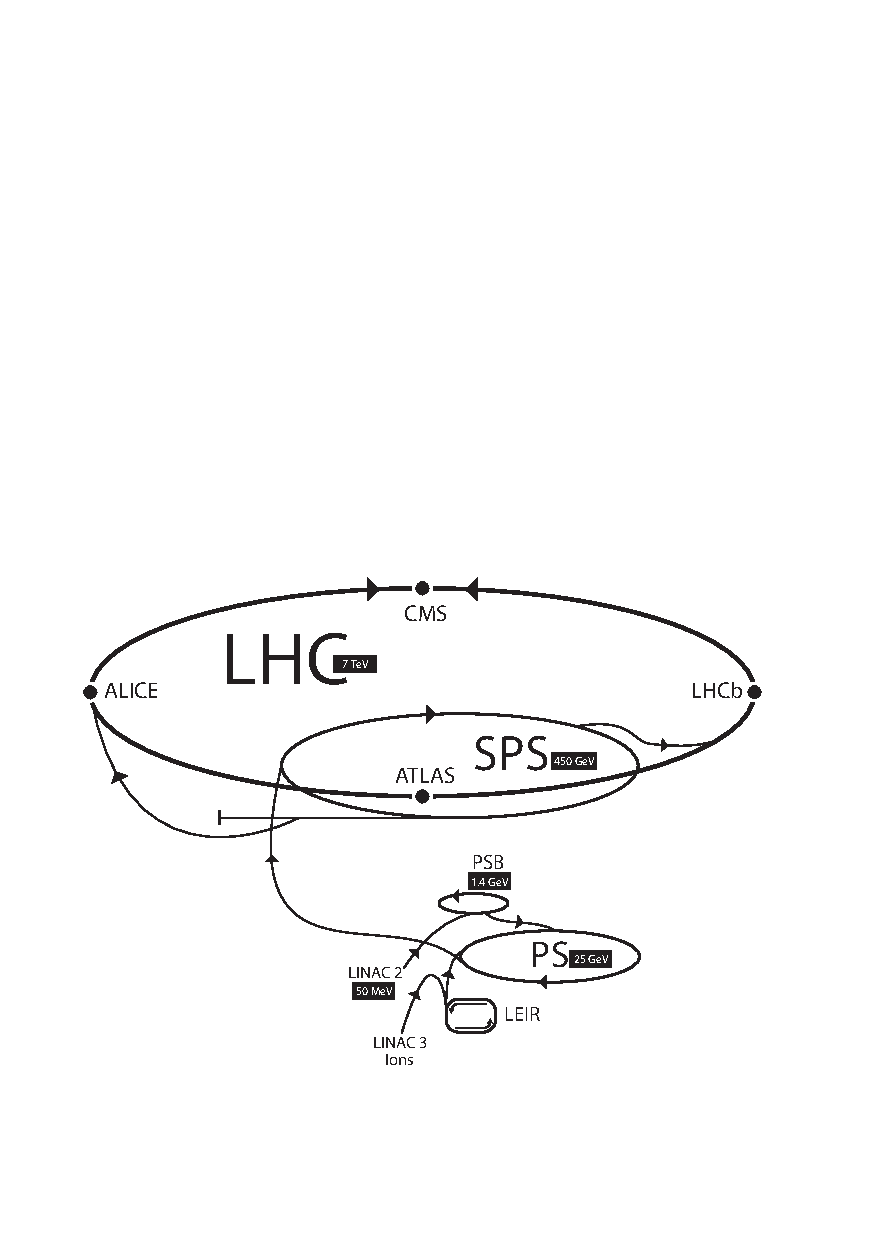
\includegraphics[width=0.48\columnwidth]{chapter3/figs/cern.pdf}
\caption[The \lhc ring.]{A illustration of the the \lhc accelerator complex showing each of the stages in the injection chain 
 for the \lhc ring along with the four main experiments on the \lhc ring~\cite{Lefevre:1092437}. ~\label{fig:lhccomplex} }
\end{figure}
It starts with a linear accelerator which accelerates the protons from rest to 50\mev. 
The synchrotrons increase the beam energy and refine the proton bunches to a configuration suitable for the \lhc. 
Firstly the Proton Synchrotron Booster (PSB) takes the beam from 50\mev to 1.5\gev at which point the 
beam enters the Proton Synchrotron (PS) where the beam energy is increased to 25\gev. 
The beam is then transferred to the Super Proton Synchrotron (SPS) which increases the energy to 450\gev
 before injecting the protons into the \lhc. 
The \lhc accelerates the proton bunches from injection energy at 450\gev to the final collision energy, which was 3.5\tev per beam in 2011 and 4\tev per beam in 2012.
Consolidation upgrades of the \lhc to take place in 2013 and 2014 are expected to increase this collision energy to the design energy of 7\tev per beam.
During operation in 2011-12 there were 1380 proton bunches per beam with a bunch spacing of 50\ns.
There are four main experiments on the \lhc ring, two general purpose detectors (\atlas and \cms), 
along with a heavy-ion experiment (\alice) and a dedicated B-physics experiment (\lhcb).

At the \lhcb interaction point the instantaneous luminosity of the colliding proton bunches 
 is constant at around $\lum\approx3\times10^{32}\cm^2\sec^{-1}$. 
This is significantly below the  \lhc  luminosity, which in 2011 reached over $\lum\approx1\times10^{33}\cm^2\squark^{-1}$.
This luminosity was chosen so that the number of interactions per proton bunch crossing ($\mu$) 
stayed uniform throughout the period of proton collisions for each `fill' of the \lhc.
This ensures that the environment is consistent and has a low multiplicity for reconstruction of \B mesons 
but that there is still a sufficient number of \B meson decays of interest for a given number of collisions.

The production of \bbbar pairs in $pp$ interactions is governed predominantly 
by gluon fusion, $gg\to\bbbar$.
The collision of partons of unequal energy and a momentum boost along the direction of the collision results in \bbbar pairs 
that are produced at small angles to the beam axis.
The angular distribution of \bbbar production is shown in Fig.~\ref{fig:lhcb:bbbar}.
\begin{figure}[tbp]
\centering
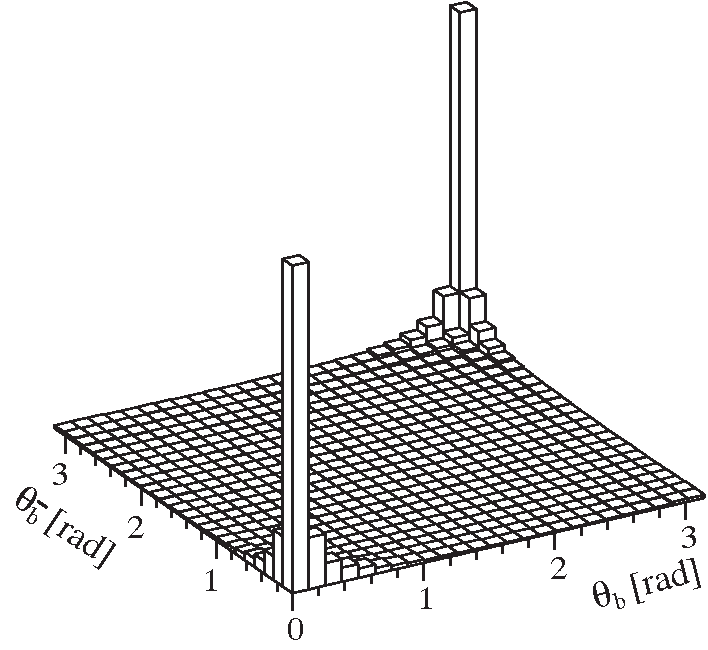
\includegraphics[width=0.48\columnwidth]{chapter3/figs/angular.pdf}
\caption[ $b\bar{b}$ production at the LHC ]{The angular distribution of \bbbar pairs in terms of the polar angle from the beam axis.
The \bbbar pairs are largely produced within a very small opening angle hence the development of \lhcb as a forward spectrometer
~\cite{Alves:2008zz}.~\label{fig:lhcb:bbbar} }
\end{figure}
The \bbbar cross section at \sqs=7\tev is 75\mub within the \lhcb acceptance~\cite{LHCb-PAPER-2010-002}. 
%This corresponds to around $10^7$ \bbbar pairs produced in the 2011 year of data-taking.
In total the experiment recorded an integrated luminosity of 1.0\invfb in 2011 that could be used for further analysis.
The increase in integrated luminosity throughout the year can be seen in Fig.~\ref{fig:lhcb:intlumi} along with the technical stops
 and periods of machine development.
\begin{figure}
\centering
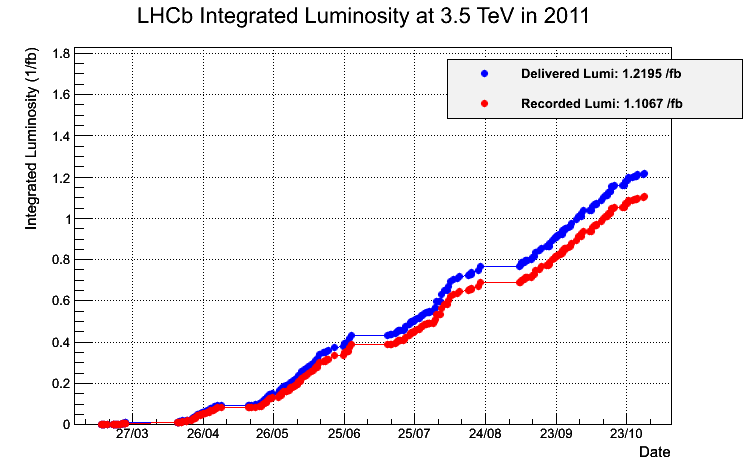
\includegraphics[width=0.66\columnwidth]{chapter3/figs/2011IntegratedLumiLHCbTime_NoPie.png}
\caption{The integrated luminosity recorded by \lhcb during 2011~\cite{OpsPlots}.~\label{fig:lhcb:intlumi} }
\end{figure}


\section{Selection of \BdToKpimm candidates}

\subsection{Data}
\label{sec:swave:meas:data}

The measurement of the S-wave contribution to \BdToKpimm was performed on the complete dataset collected at \lhcb in 2011.
This was the identical dataset used in the second angular analysis presented in Chapter~\ref{chap:kstmm} and 
corresponds to an integrated luminosity of 1.0\invfb at $\sqs=7\tev$. 
The data are described in more detail in Section~\ref{sec:kstmm:data}.

The simulation samples that were used in this measurement consist of the samples already described in Section~\ref{sec:kstmm:data:mc} 
along with an additional sample of \BdToKpimm events.
This additional simulation sample was generated uniformly in phase space and in the MC11 configuration
 using the \lhcb simulation as described in Sec.~\ref{sec:lhcb:soft}.
This simulation was used to understand the efficiency in the wide \kpi mass range.

The data-simulation corrections developed in Sec~\ref{sec:kstmm:data:mccorr} were applied to all of the simulation samples in order to ensure
 that the efficiency calculations were as accurate as possible.



\subsection{Selection}
\label{sec:swave:meas:sel}

The selection of signal \BdToKpimm events was based on the selection presented 
in Section~\ref{sec:kstmm:sel} for \BdToKstmm candidates.
The allowed mass range of \kpi candidates was widened to include the \kpi threshold at $634\mev$ up to $1200\mev$.
This is because there are regions of almost pure S-wave either side of the $\Kstarzo(892)$ as described in Sec~\ref{sec:swave:theo} 
but this range avoids interference from the $\Kstarzt(1430)$.
A cut-based selection was used to remove peaking background events before a multi-variate algorithm
was used to select a pure sample of \BdToKpimm events.

However, this expansion of the \kpi mass window necessitated a 
re-examination of parts of the selection for the angular analysis of \BdToKstmm. 
The vetoes for possible peaking backgrounds, such as the \ktopi swaps and other exclusive \bquark decays,
must also work in the wider \kpi mass window.
In order to select a clean sample of \BdToKpimm candidates, the same multivariate algorithm was 
used to separate potential signal candidates and the remaining combinatorial background.
The selection of \BdToJpsiKpi events was achieved using the same selection but by specifically selecting the \qsq region between 8 and 10 \gevgevcccc
as described in Section~\ref{sec:kstmm:sel}.

\subsection{Peaking backgrounds}

\subsubsection{\ktopi swaps}

Candidates which cannot be separated through hadron identification are called \ktopi swaps because they pass the selection 
with reasonable kaon and pion identification when  the kaon and pion masses are swapped.
These `swaps' manifest as duplicate candidates and require vetoing to avoid double counting.
These \ktopi swaps were vetoed in Section~\ref{sec:kstmm:sel} under two conditions. 
The invariant mass of the \kpi pair with the pion and kaon masses exchanged must have fallen in the \kpi window
and the hadron identification values must have satisfied the condition that the difference between the \dllkpi for the kaon (\kdllkpi) and the pion (\pidllkpi) was greater than minus ten.
However, this condition fails to veto sufficient candidates in the wide \kpi window. 

The distribution of \ktopi swaps in terms of \kdllkpi and \pidllkpi for selected \BdToKpimm candidates
is given in Fig.~\ref{fig:swave:meas:kpiswaps}. 
\begin{figure}[tbp]
\centering
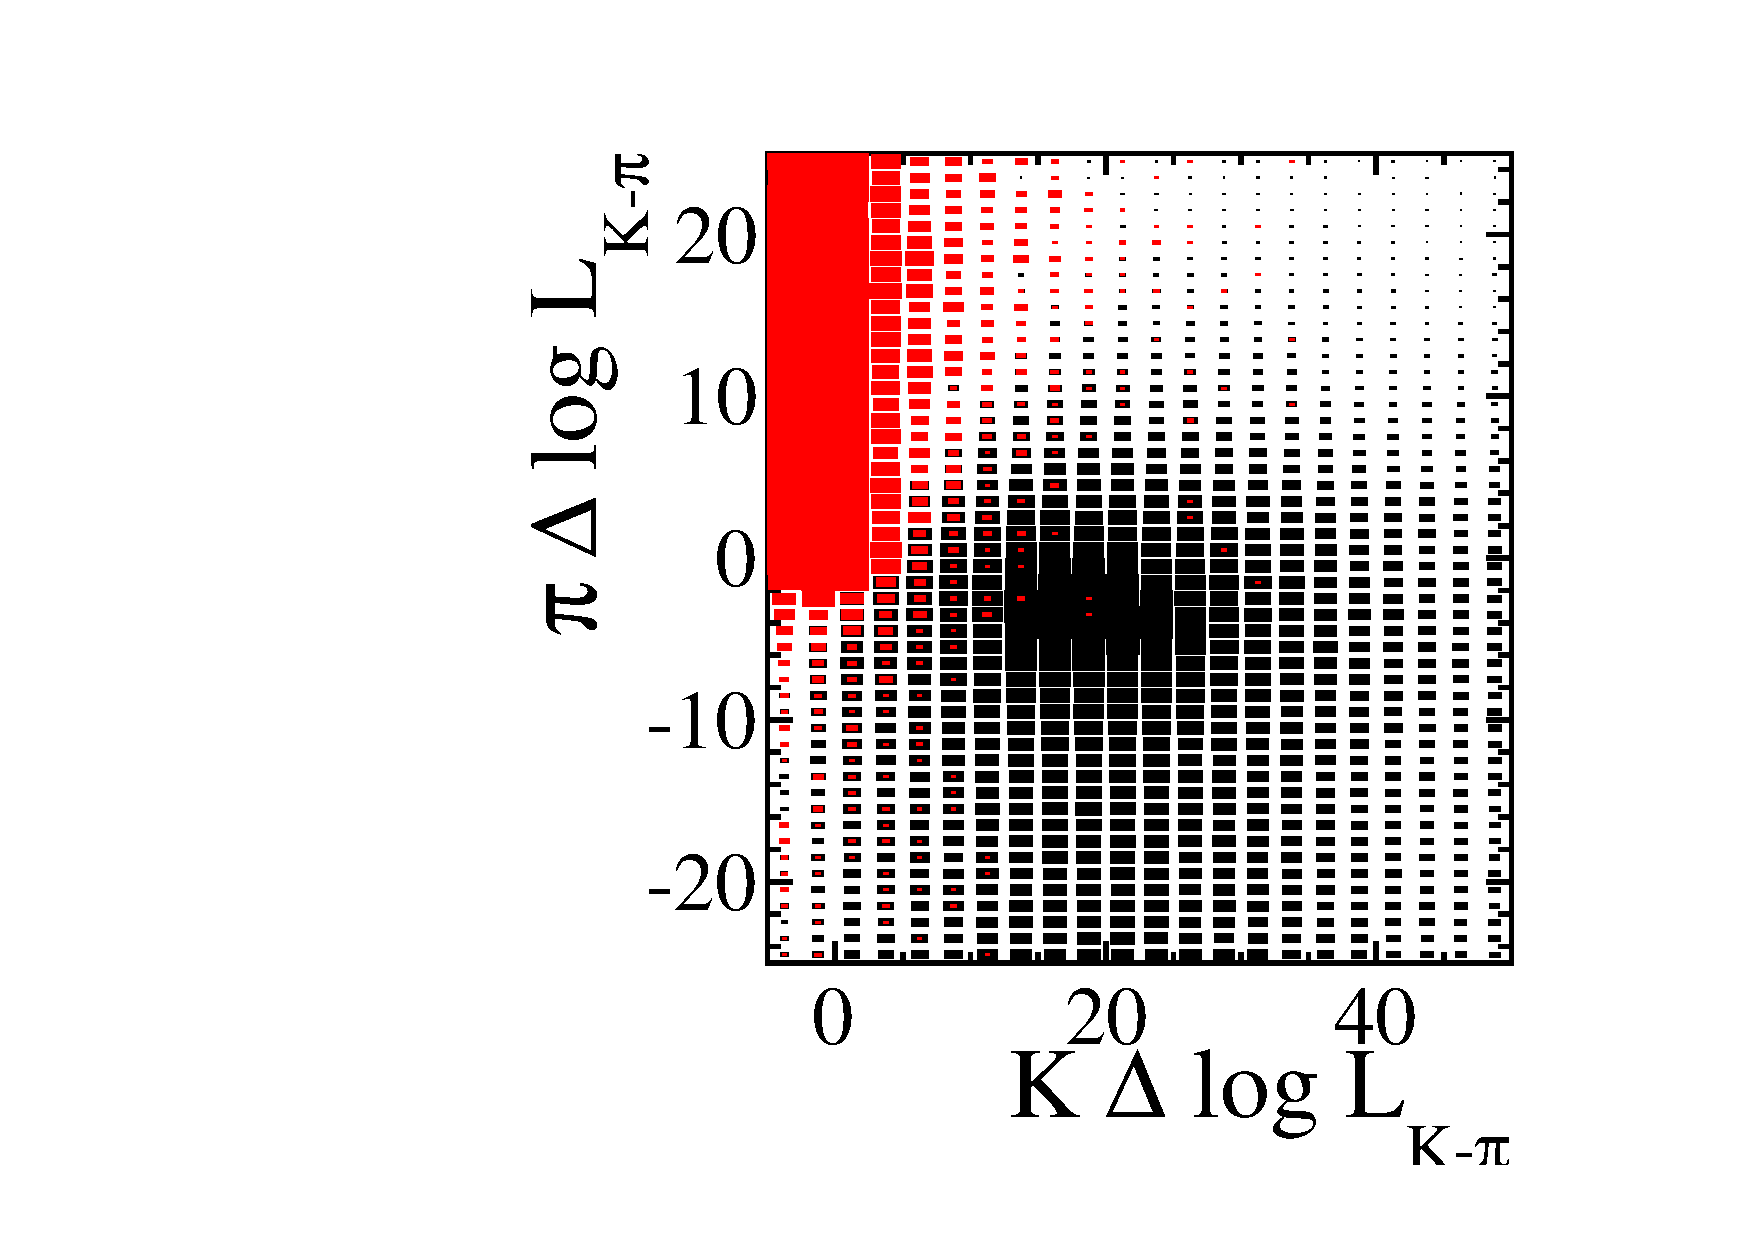
\includegraphics[width=0.48\columnwidth]{chapter7/figs/kstarmumu_swap_2Ddist.pdf}
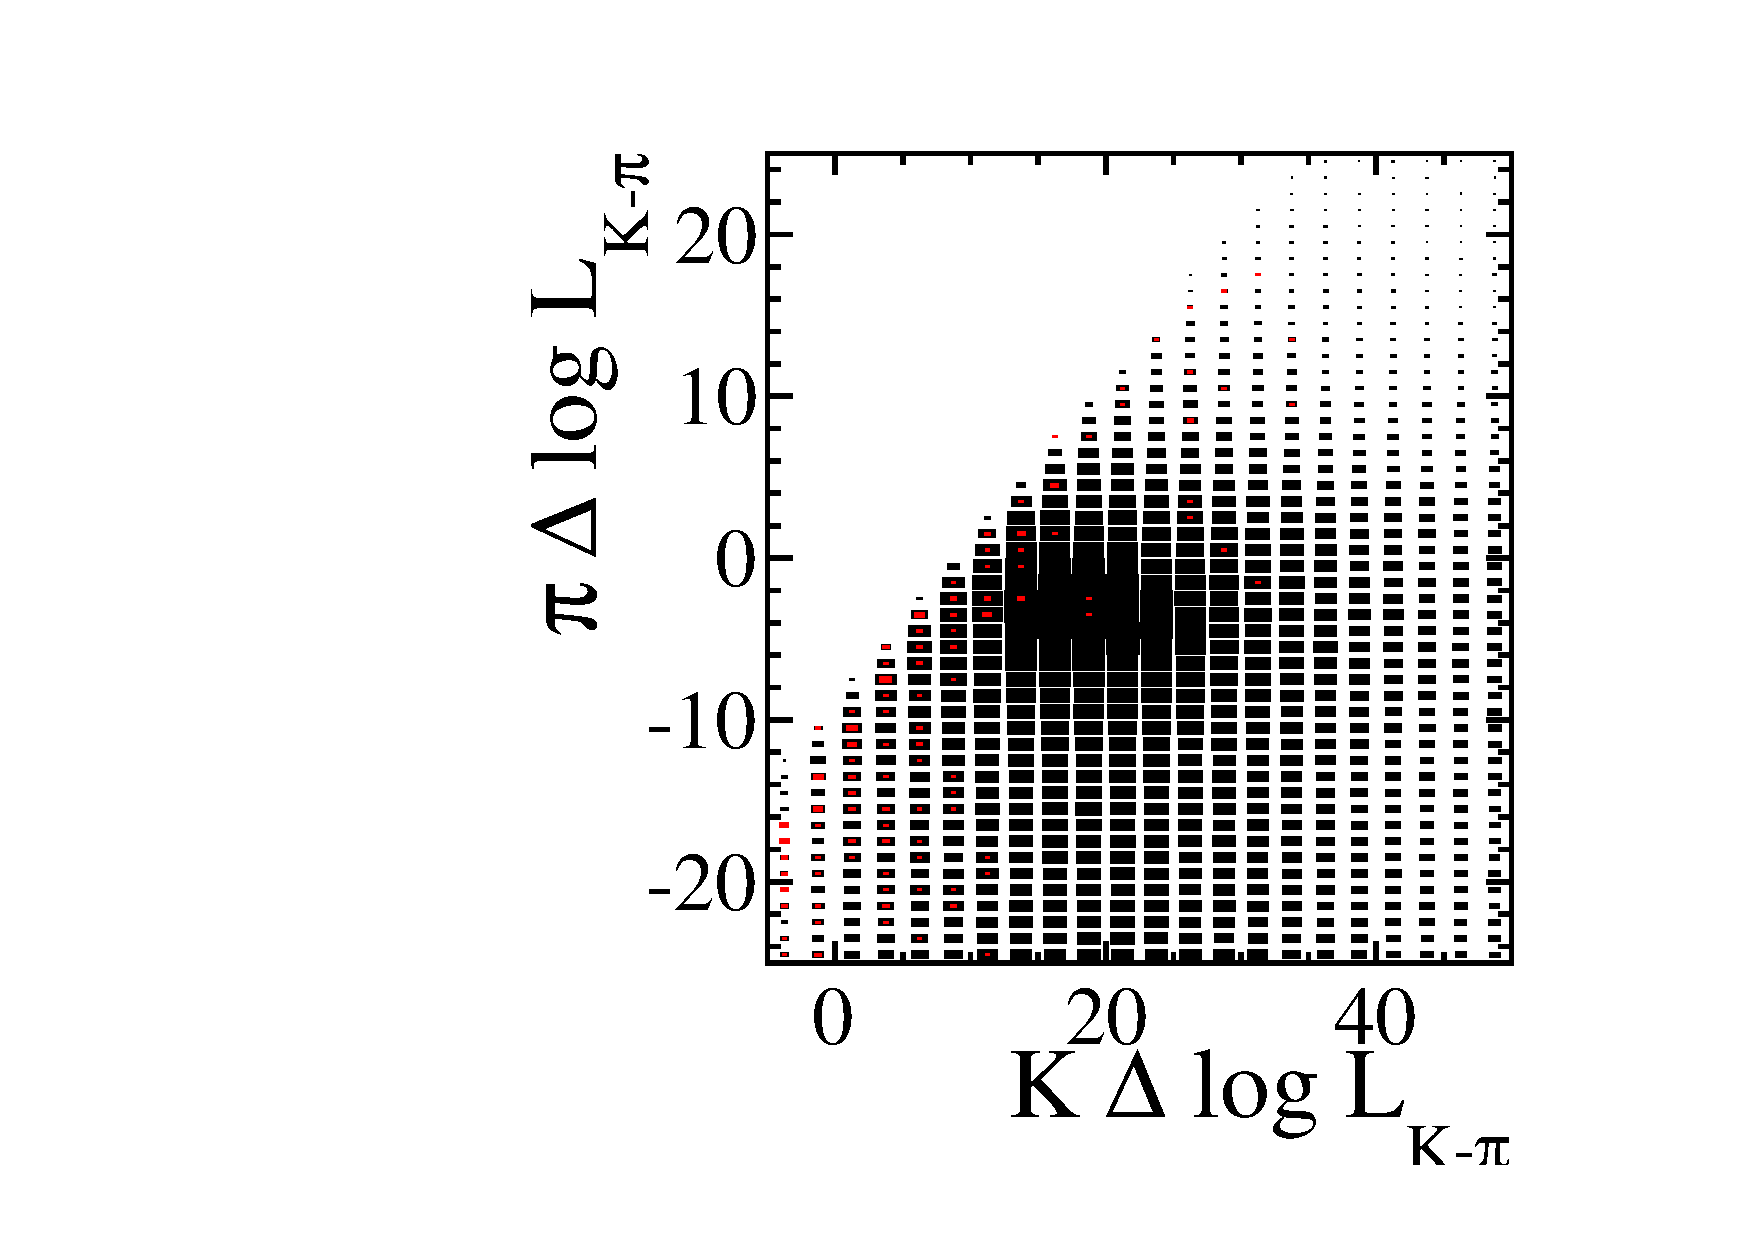
\includegraphics[width=0.48\columnwidth]{chapter7/figs/kstarmumu_swap_2Ddist_veto.pdf}
\caption[  The distribution of \BdToKpimm simulation (a) before and (b) after the \ktopi swap veto.   ]
{The distribution of \BdToKpimm simulation (a) before and (b) after the \ktopi swap veto. 
Candidates with the correction assignment of masses for the kaon and pion are shown in black and candidates 
with the incorrect assignment of masses are shown in red. There is a clear overlap of candidates around \dllkpi of 0 for both particles.
~\label{fig:swave:meas:kpiswaps} }
\end{figure}
The overlap of the two distributions can be seen around the zero point motivating the use of the diagonal cut, $\kdllkpi-\pidllkpi>10$.
The efficiency of the swap veto is around 92\% on signal events which pass the multivariate selection and 
less than 2.5\% of swapped candidates are retained after the veto.
There are less than 0.1\% of \ktopi swap candidates in the simulation after selection.

\subsubsection{Other peaking backgrounds}

The possible sources of peaking backgrounds considered have a % are also considered in Section~\ref{sec:kstmm:sel} and
mass close to the \Bd mass after the misidentification of one or more of the final state particles
 and could create structure in the \kpi mass spectrum. They are
\begin{itemize}
\item \BdToKstmm with the pion misidentified as the muon and the muon as the pion.
\item \BdToKstmm with the kaon misidentified as the muon and the muon as the kaon.
\item \BsToPhimm with one of the kaons misidentified as a pion.
\item \BuToKmm with an added soft pion.
\item \LbToLmm (1) with the proton misidentified as a pion.
\item \LbToLmm (2) with the proton misidentified as a kaon and the kaon misidentified as a pion.
\end{itemize}
In order to understand the \kpi mass distribution of these exclusive backgrounds, 
simulation samples for each decay were used. % generated and corrected as described in Section~\ref{sec:kstmm:data:mccorr} .
Each simulation sample was weighted so that the number of events in the sample was equivalent to the expected yield from 1.0\invfb of data.
The number of events after selection for the signal \Bd and \kpi mass region, the signal \Bd and the wide \kpi mass region
 and the wide \Bd and the wide \kpi mass region are shown in Table~\ref{tbl:peaking:backgrounds}.
\begin{table}
\centering
\caption[   The expected number of peaking background events from selected simulated data in three different mass ranges
for an integrated luminosity of 1.0\invfb.   ]
{ The expected number of peaking background events from selected simulated data in three different mass ranges
for an integrated luminosity of 1.0\invfb. The assumed branching fraction is given in the first column.
The first mass range is from $5230<\mB<5330\mevcc$ and $800<\mkpi<1000\mevcc$. 
The second mass range is from $5230<\mB<5330\mevcc$ and $634<\mkpi<1200\mevcc$ 
The third range mass range is from $5200<\mB<5700\mevcc$, $634<\mkpi<1200\mevcc$. 
The errors are statistical.~\label{tbl:peaking:backgrounds} }
\begin{tabular}{|c|c|c|c|c|}
\hline
Background  & $\Gamma$  & Range 1 & Range 2 & Range 3 \\
\hline
\BdToKstmm ( $K\leftrightarrow\pi$ )  &   $1.0\times10^{7}$&  $ 0.119\pm0.345 $ &$ 0.158\pm0.397 $ &$ 0.487\pm0.698 $ \\ 
\BdToKstmm ( $\pi\leftrightarrow\mu$ )  & $1.0\times10^{7}$&  $ 0.5\pm0.707 $ &$ 1.5\pm1.22 $ &$ 2.33\pm1.53 $ \\ 
\BdToKstmm ( $K\leftrightarrow\mu$ ) &    $1.0\times10^{7}$&  $ 0\pm0 $ &$ 0\pm0 $ &$ 0\pm0 $ \\ 
\BsToPhimm  &                             $5.5\times10^{7}$&  $ 3.1\pm1.76 $ &   $ 5.93\pm2.44 $ &$ 7.91\pm2.81 $ \\ 
\BuToKmm  &                               $6.0\times10^{7}$&  $ 0.0851\pm0.292 $ &  $ 0.17\pm0.413 $ &$ 1.3\pm1.14 $ \\ 
\LbToLmm (1)  &                           $1.0\times10^{7}$&  $ 13.2\pm4.63 $ &   $ 25.1\pm7.01 $ &$ 79.7\pm10.93 $ \\ 
\LbToLmm (2) &                            $1.0\times10^{7}$&  $ 3.8\pm2.95 $ &$ 6.82\pm3.61 $ &$ 13.3\pm5.64 $ \\  
\hline
\end{tabular}
\end{table}
%As measured in Section~\ref{sec:kstmm:res}, there are 900 \BdToKstmm candidates in the 1.0\invfb data. 
%This means that most of the peaking backgrounds are around 1\% or less in the signal region, 
%justifying their ignorance in the previous measurement.
%However, there are larger contributions from the peaking backgrounds in the high \kpi mass region and the higher \Bd mass region.
The distribution of peaking background simulation is given in figure~\ref{fig:swave:peaking:backgrounds}.
\begin{figure}
\centering
\subfigure[]{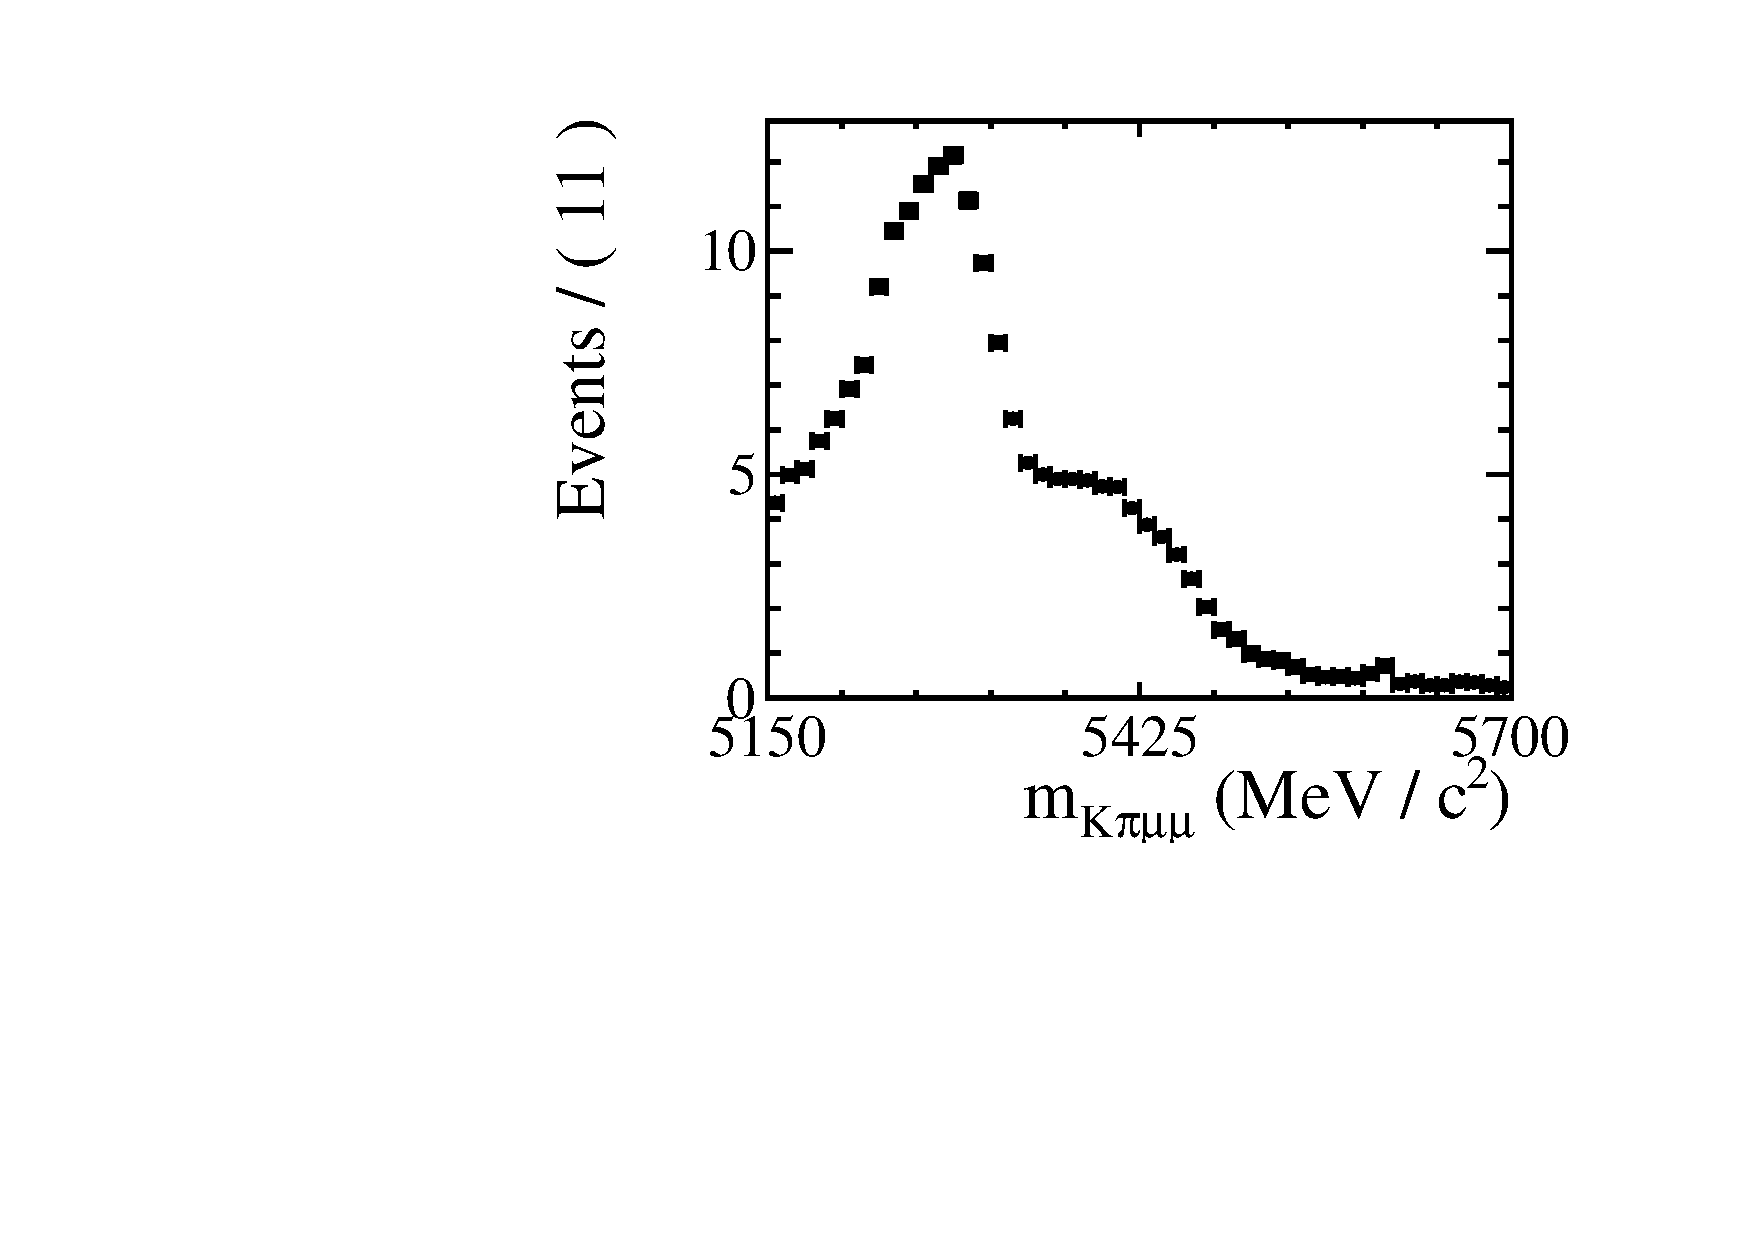
\includegraphics[width=0.32\columnwidth]{chapter7/figs/peaking/peaking_backgrounds_mass.pdf}}
\subfigure[]{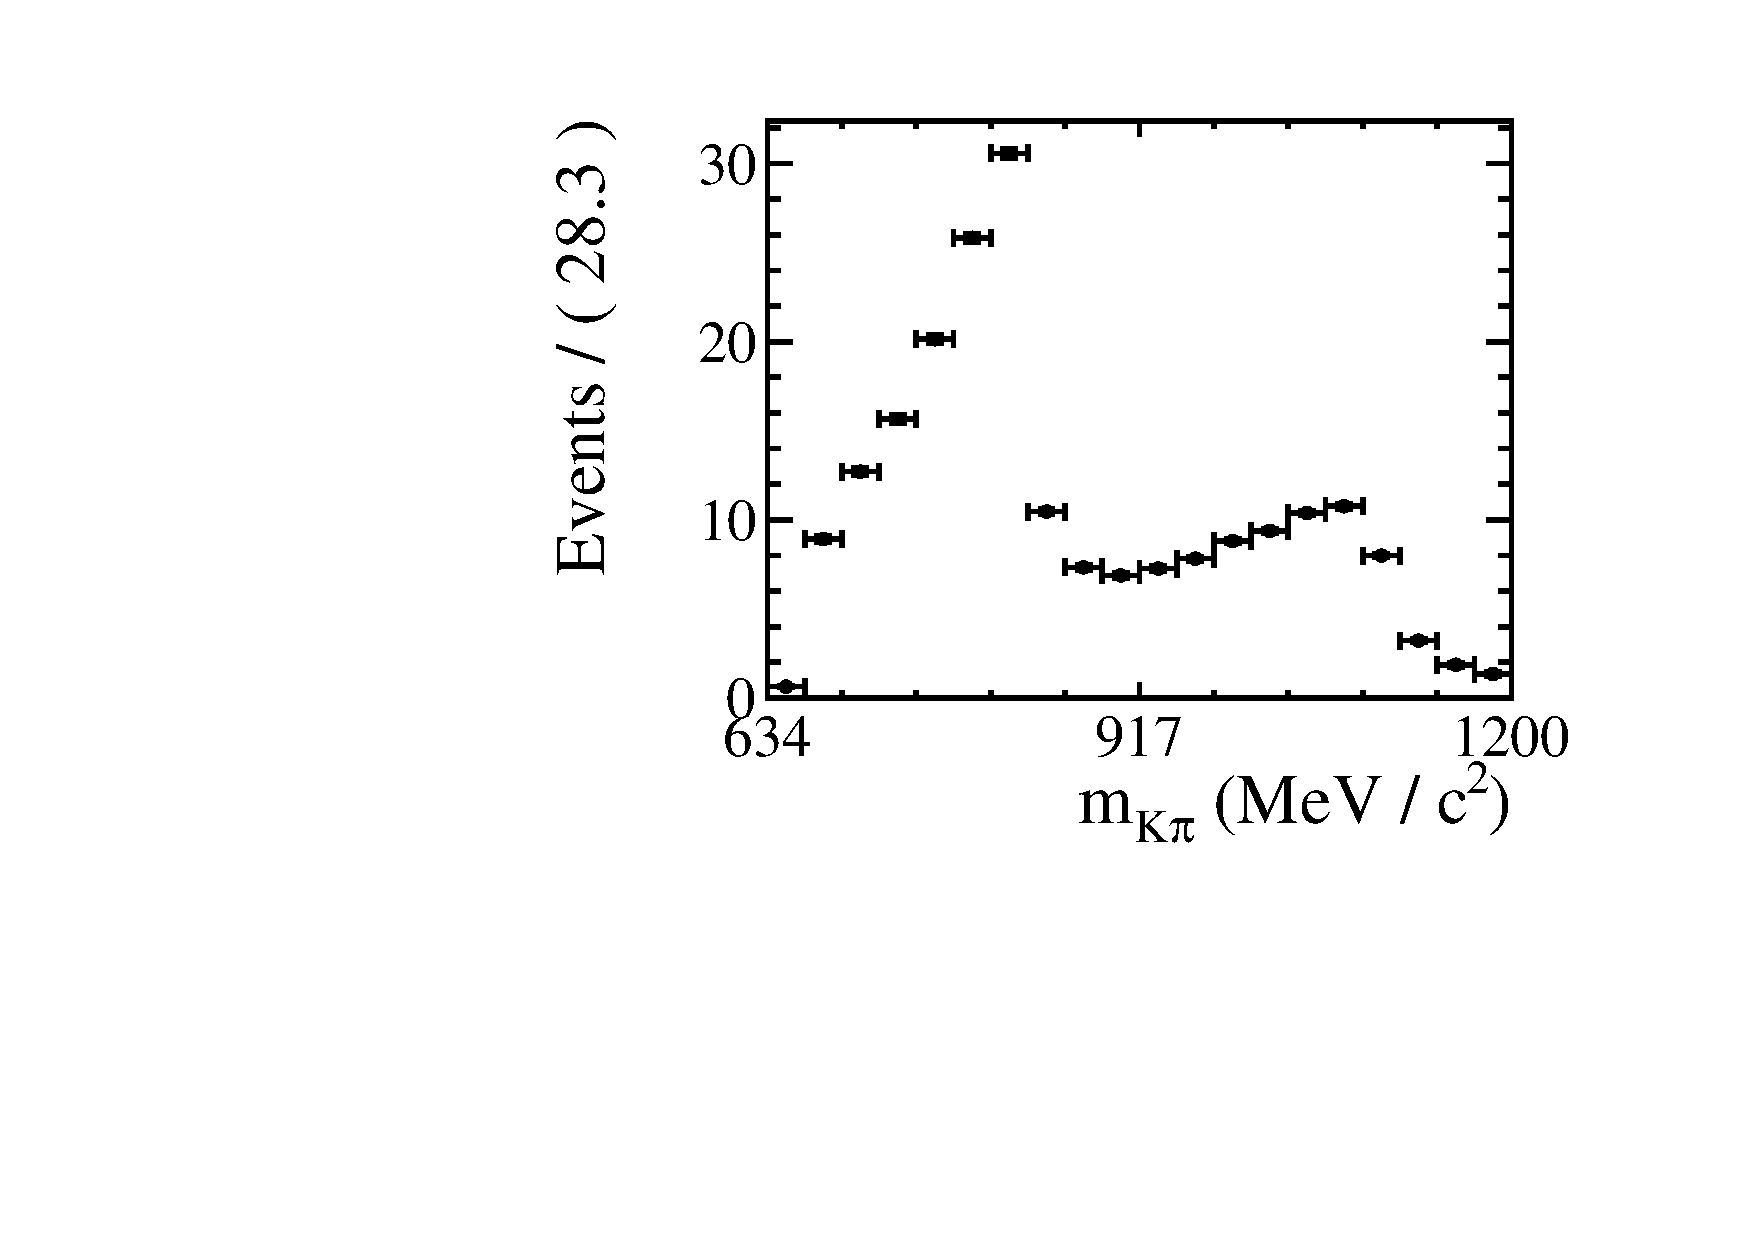
\includegraphics[width=0.32\columnwidth]{chapter7/figs/peaking/peaking_backgrounds_mkpi.pdf}}
\subfigure[]{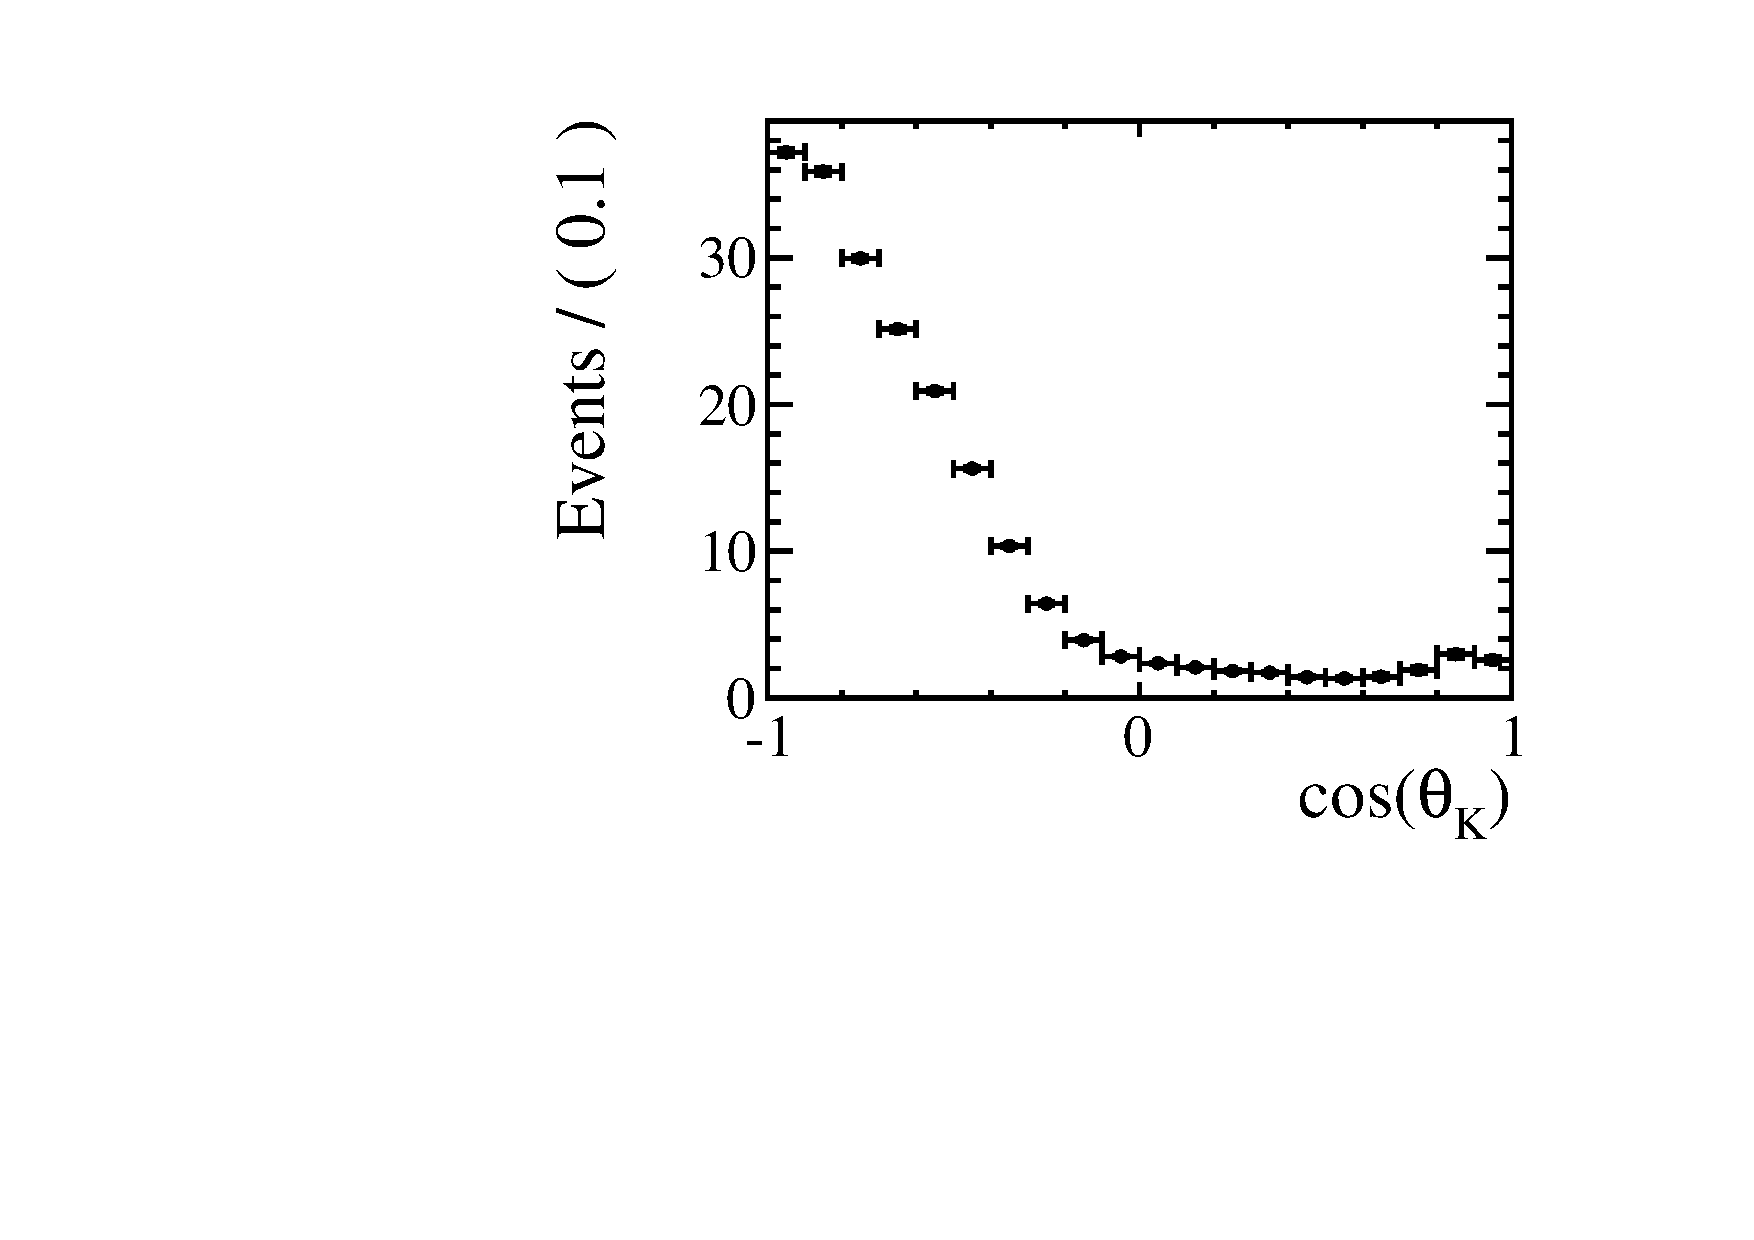
\includegraphics[width=0.32\columnwidth]{chapter7/figs/peaking/peaking_backgrounds_ctk.pdf}}
\caption[ The combined distribution of peaking background events after selection in terms of (a) \mkpimm, (b) \mkpi and (c) \ctk.   ]
{ The combined distribution of peaking background events after selection in terms of (a) \mkpimm, (b) \mkpi and (c) \ctk.
The distribution is composed of simulated \BdToKstmm, \BsToPhimm, \BuToKmm and \LbToLmm normalised to
the expected number of events in 1.0\invfb of data. %It is possible to see non-trivial shapes 
%in the \kpimm and \kpi mass distributions.% but the number of events is almost insignificant.
~\label{fig:swave:peaking:backgrounds} }
\end{figure}
It is possible to see structure in each of the \mkpill, \mkpi and \ctk distributions.
However, the fraction of peaking background events in the \kpill mass window is less than $(2.0\pm0.2)\%$ after the selection allowing these contributions to be ignored under the P-wave peak.

%\subsection{Data distributions}
%The distribution of selected \BdToKpimm and \BdToJpsiKpi candidates as a function of \mB and \mkpi are shown in Fig.~\ref{fig:swave:mass:mkpi}.
%Here the \mkpi window is extended upwards to 2000\mev to show the overall distribution of events at high \mkpi.
%\begin{figure}[tbp]
%\centering
%\subfigure[]{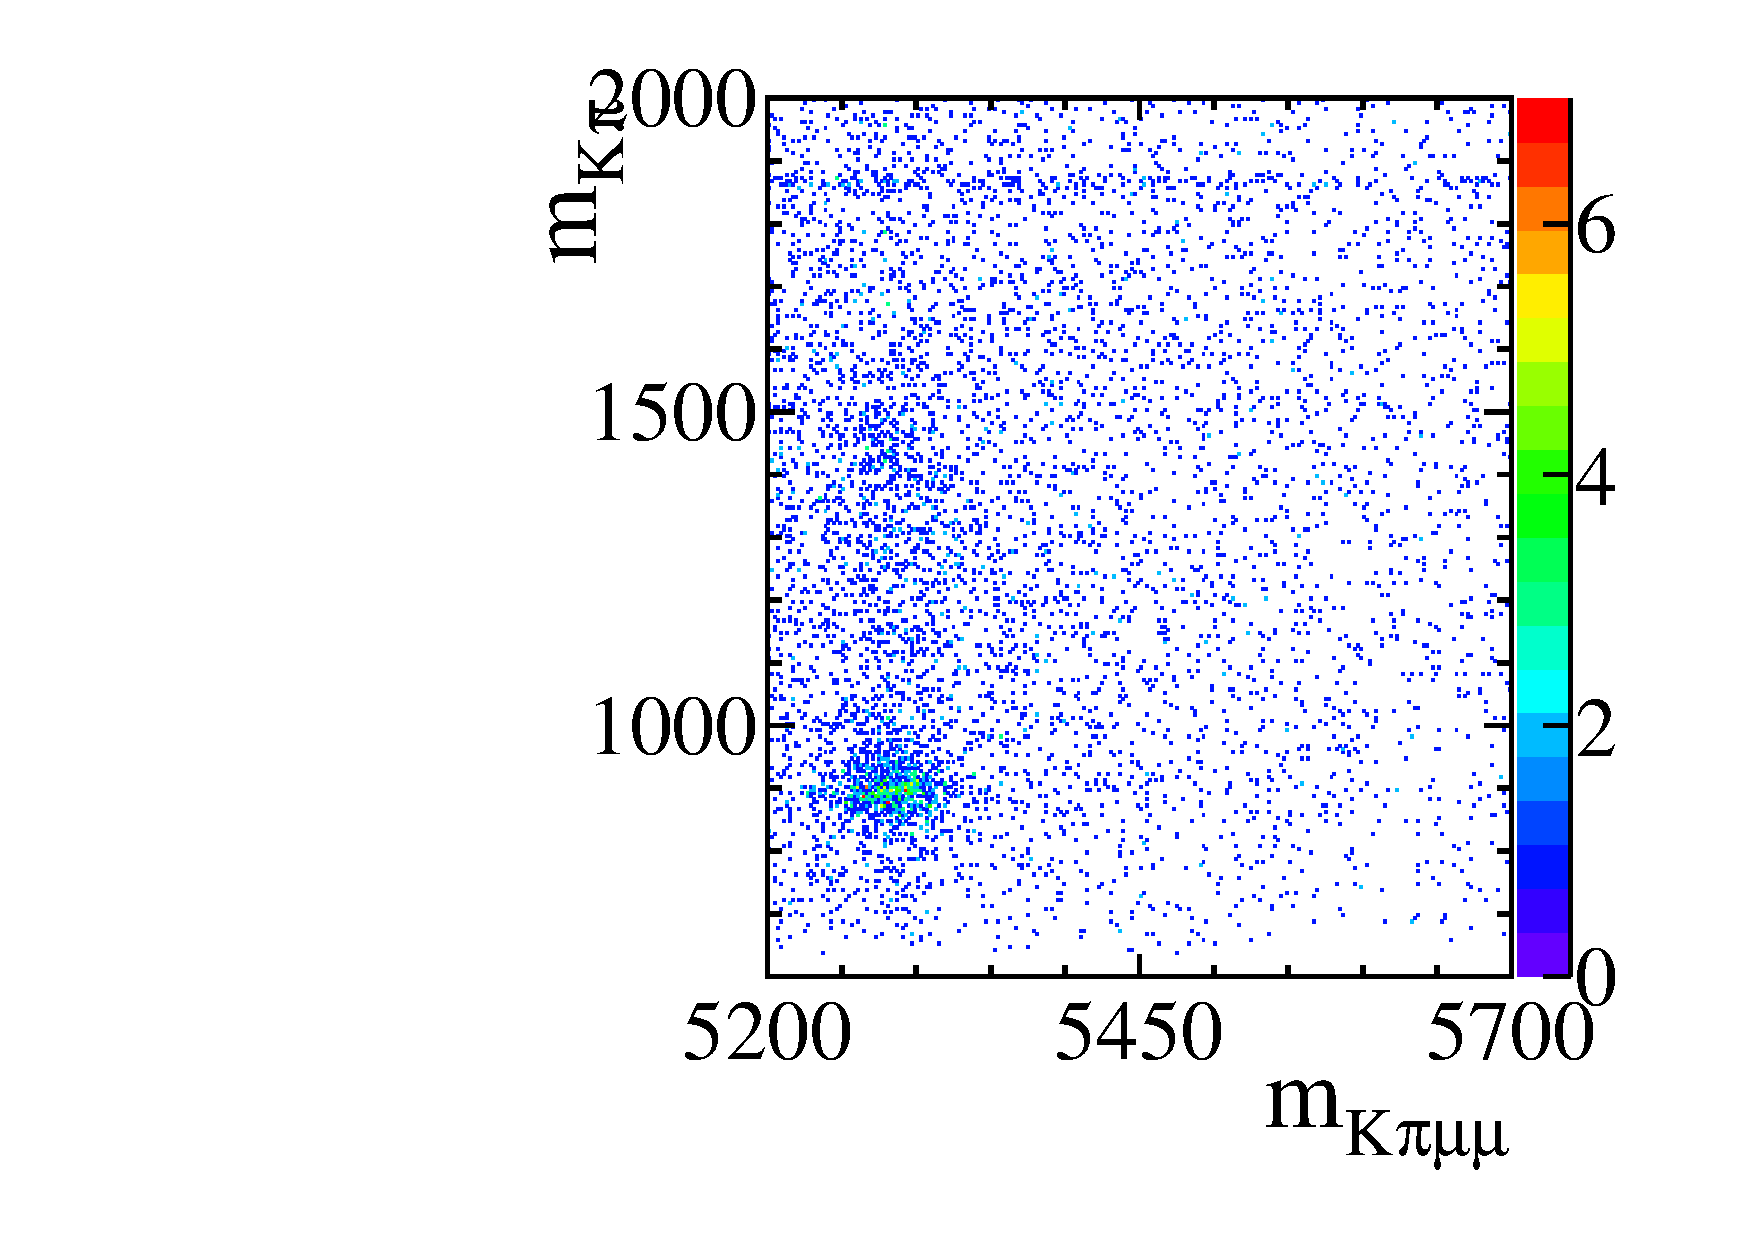
\includegraphics[width=0.48\columnwidth]{chapter7/figs/massdists_kstarmumu_mB_mkpi.pdf}}
%\subfigure[]{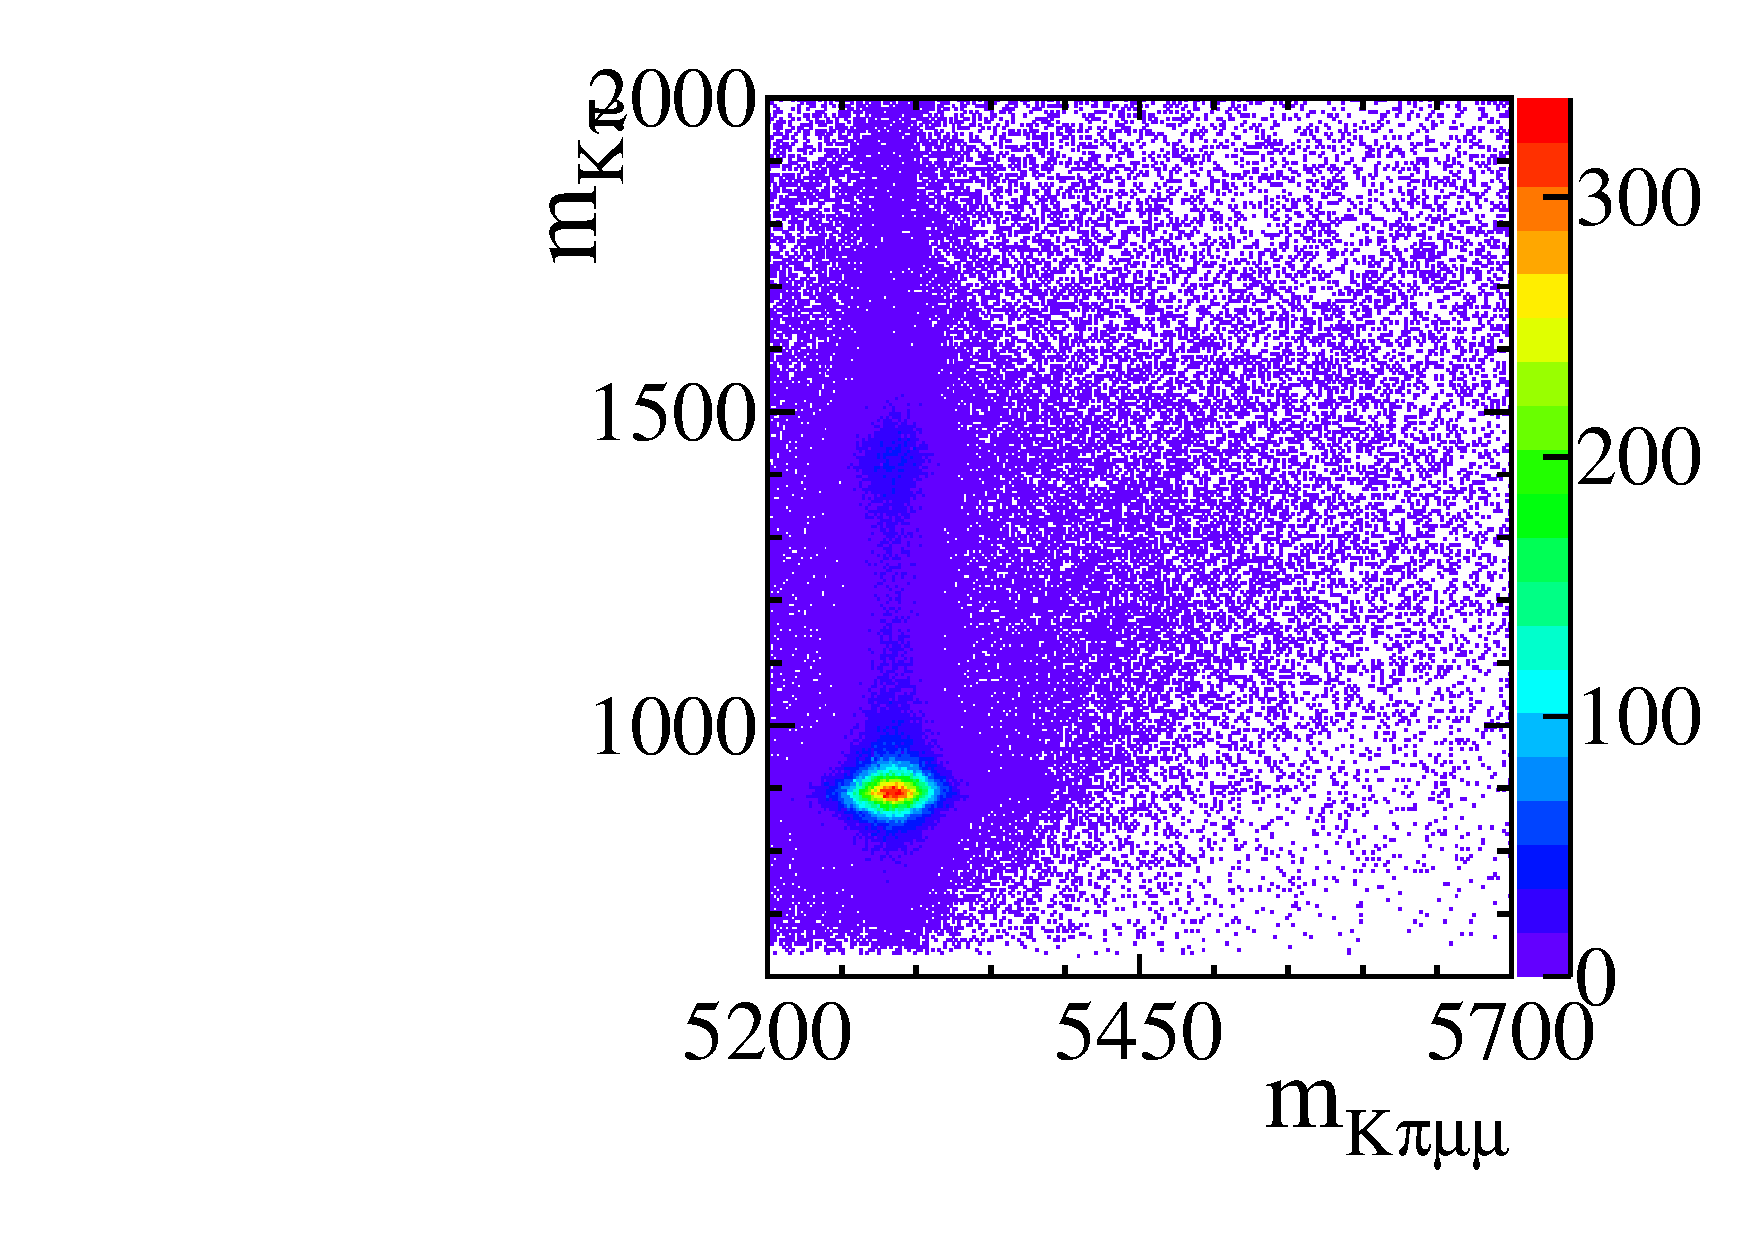
\includegraphics[width=0.48\columnwidth]{chapter7/figs/massdists_jpsikstar_mB_mkpi.pdf}}
%\caption{ \mB v.s. \mkpi mass distributions for the wide \mkpi region for (a) \BdToKstmm and (b) \BdToJpsiKstar. 
%In the \BdToKstmm selection, it is possible to see the P-wave clearly and a 
%combinatorial background from \D \mumu at $\mkpi\sim1800$.
%In the \BdToJpsiKstar selection, is it possible to see both the P-wave, the \kpi S-wave and a \Kstarz D-wave at 1430.
%There is also an asymmetric background in \mkpi and \mB. ~\label{fig:swave:mass:mkpi} }
%\end{figure}
%It is possible to see a clear peak of \BdToKstmm events along with a generic S-wave and 
%contributions from the $\Kstarzt(1430)$ in the \BdToJpsiKpi spectrum as described in Ref~\cite{LHCB-PAPER-2012-014}.
%There is significant difference between the high \mB background between \BdToJpsiKpi and \BdToKpimm.
%The background for the charmonium mode can be seen in increase with \mkpi indicating that it is mis-reconstructed physics background whereas the 
% \BdToKpimm background is constant as a function of \mkpi indicating that it is composed of mostly combinatorial background.






\section{Acceptance correction}
\label{sec:kstmm:ac}

The angular distribution of fully reconstructed and offline selected \BdToKstmm candidates 
is not representative of the angular distribution of \BdToKstmm events
which come from a proton-proton interaction.
This is because the process of reconstruction and selection introduces an acceptance
effect, both from the geometry of the \lhcb detector and from the reconstruction and selection
software. 
In order to perform an angular analysis, this acceptance effect must be corrected for.
There are two main approaches to including the acceptance in an angular analysis.
The acceptance can be parametrised and included in the signal \PDF and fitted to the data,
along with various external inputs to help constrain the parameters.
This approach has several benefits but it also introduces additional parameters into the fit.
Angular analyses that have used this approach include the \lhcb and \cdf measurements of $\Bd\to\jpsi\phi$~\cite{CDF:2011af,Aaij:1407836}.
As an alternative, the efficiency can be calculated in different regions of phase space to give each candidate a
weight proportional to the inverse of the efficiency,
\begin{align}
\omega(\ctl,\ctk,\phi)_i = \frac{1}{ \epsilon(\ctl,\ctk,\phi)_i } \, .
\end{align}
This method has the benefit of being separate from the result extraction, keeping the angular \PDF purely to describe the data. 
This is the method presented in this thesis and was the method used in the first two angular analyses of \BdToKstmm at \lhcb.

\subsection{Total acceptance effect on simulation}
\label{sec:kstmm:ac:effect}

Simulation was used to calculate the selection efficiency for \BdToKstmm candidates in different regions of phase space
by comparing the distribution of \BdToKstmm candidates as a function of the angular variables and \qsq
 before and after the complete selection has been applied.
The simulated events were generated as described in Section~\ref{sec:lhcb:soft} 
and corrected as described in Section~\ref{sec:kstmm:data:mccorr}.
The IP resolution and the particle identification corrections were applied before the selection. 
The distribution of the weights given to each of the simulated \BdToKstmm 
 candidates from the remaining data-simulation corrections is shown in Fig~\ref{fig:datamc:weight}.
\begin{figure}[tbp]
\centering
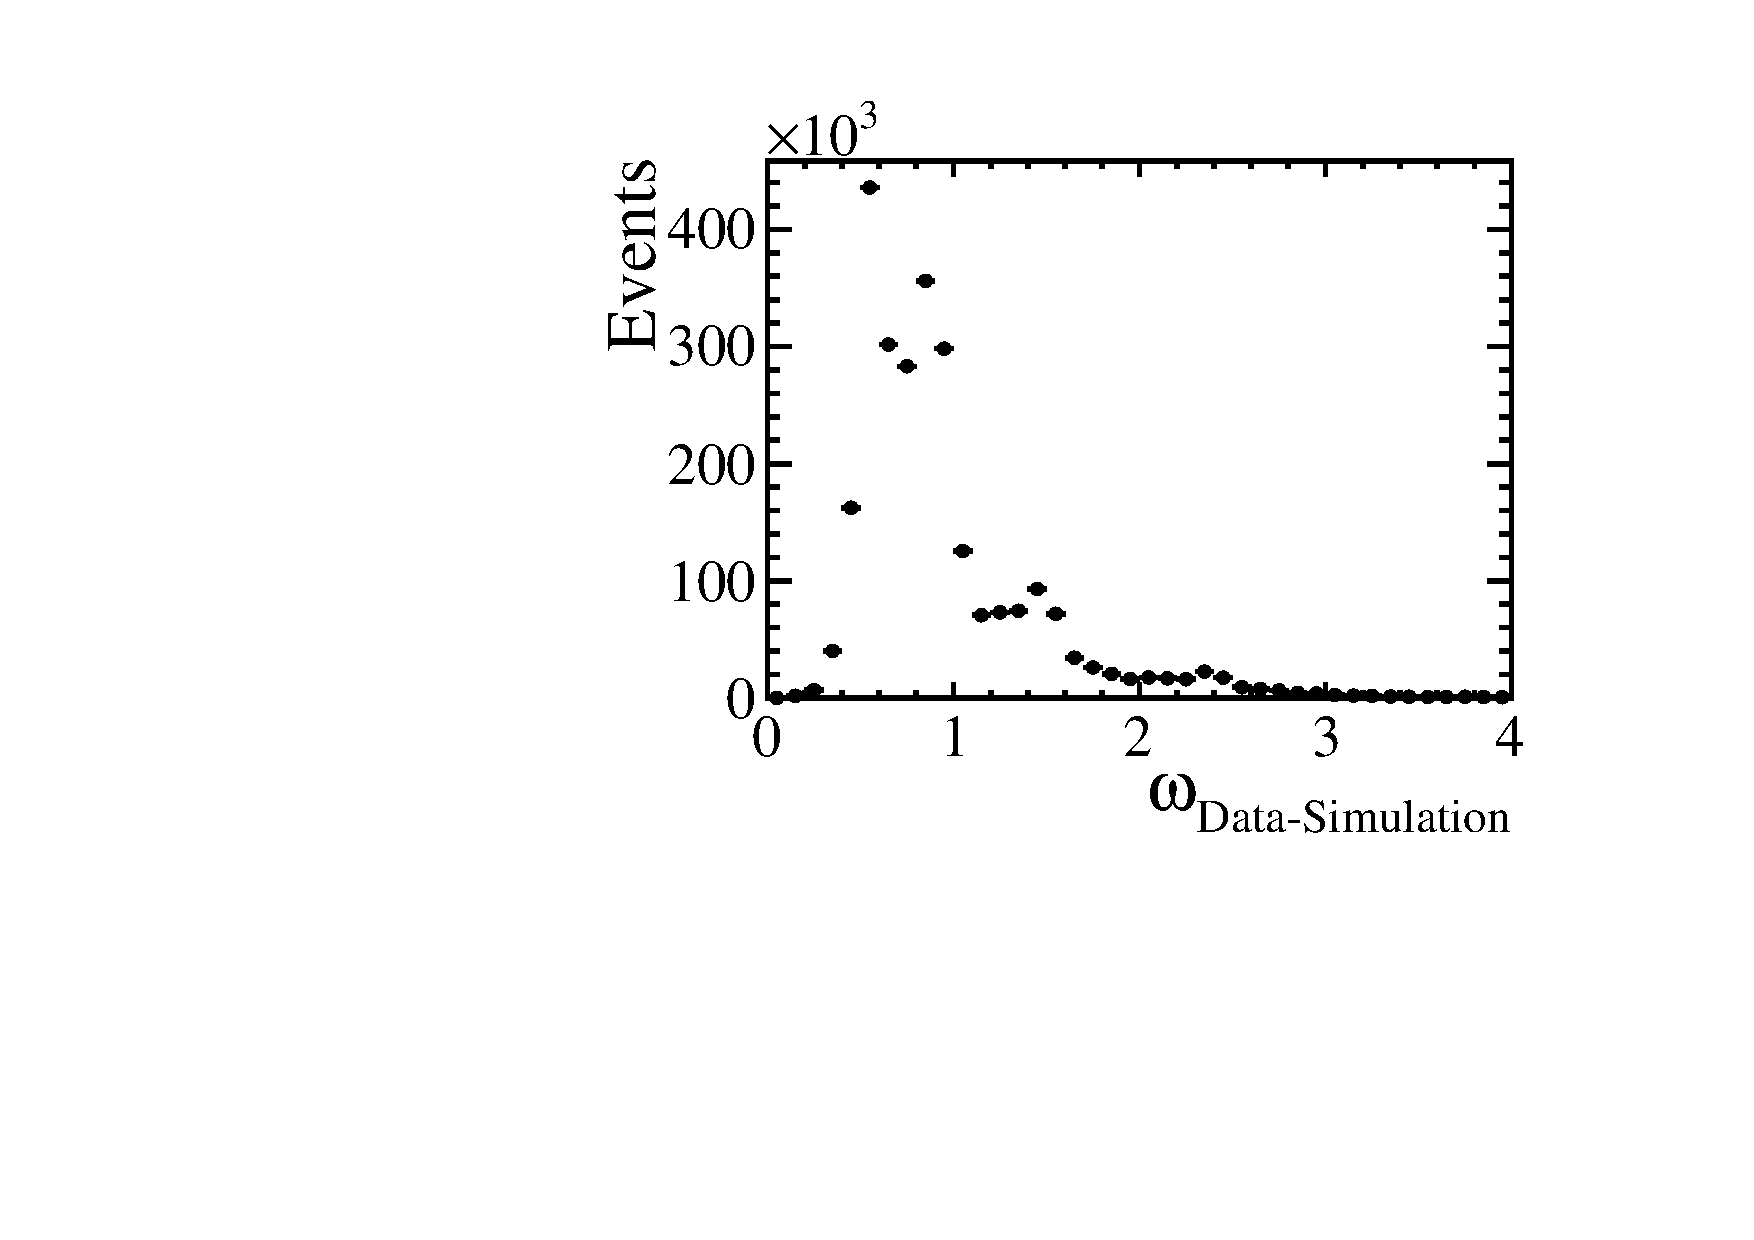
\includegraphics[width=0.48\columnwidth]{chapter5/figs/datamc/datamc_jpsikstar.pdf}
\caption{The distribution of weights to correct the simulated phase space \BdToKstmm candidates
 for known differences between the data and the simulation. ~\label{fig:datamc:weight} }
\end{figure}
The structure of four distinct peaks comes from the re-weighting for the event occupancy.

The angular distribution of fully reconstructed and selected phase space \BdToKstmm candidates
is given in Fig.~\ref{fig:phspeff}. 
\begin{figure}[tbp]
\centering
\subfigure[]{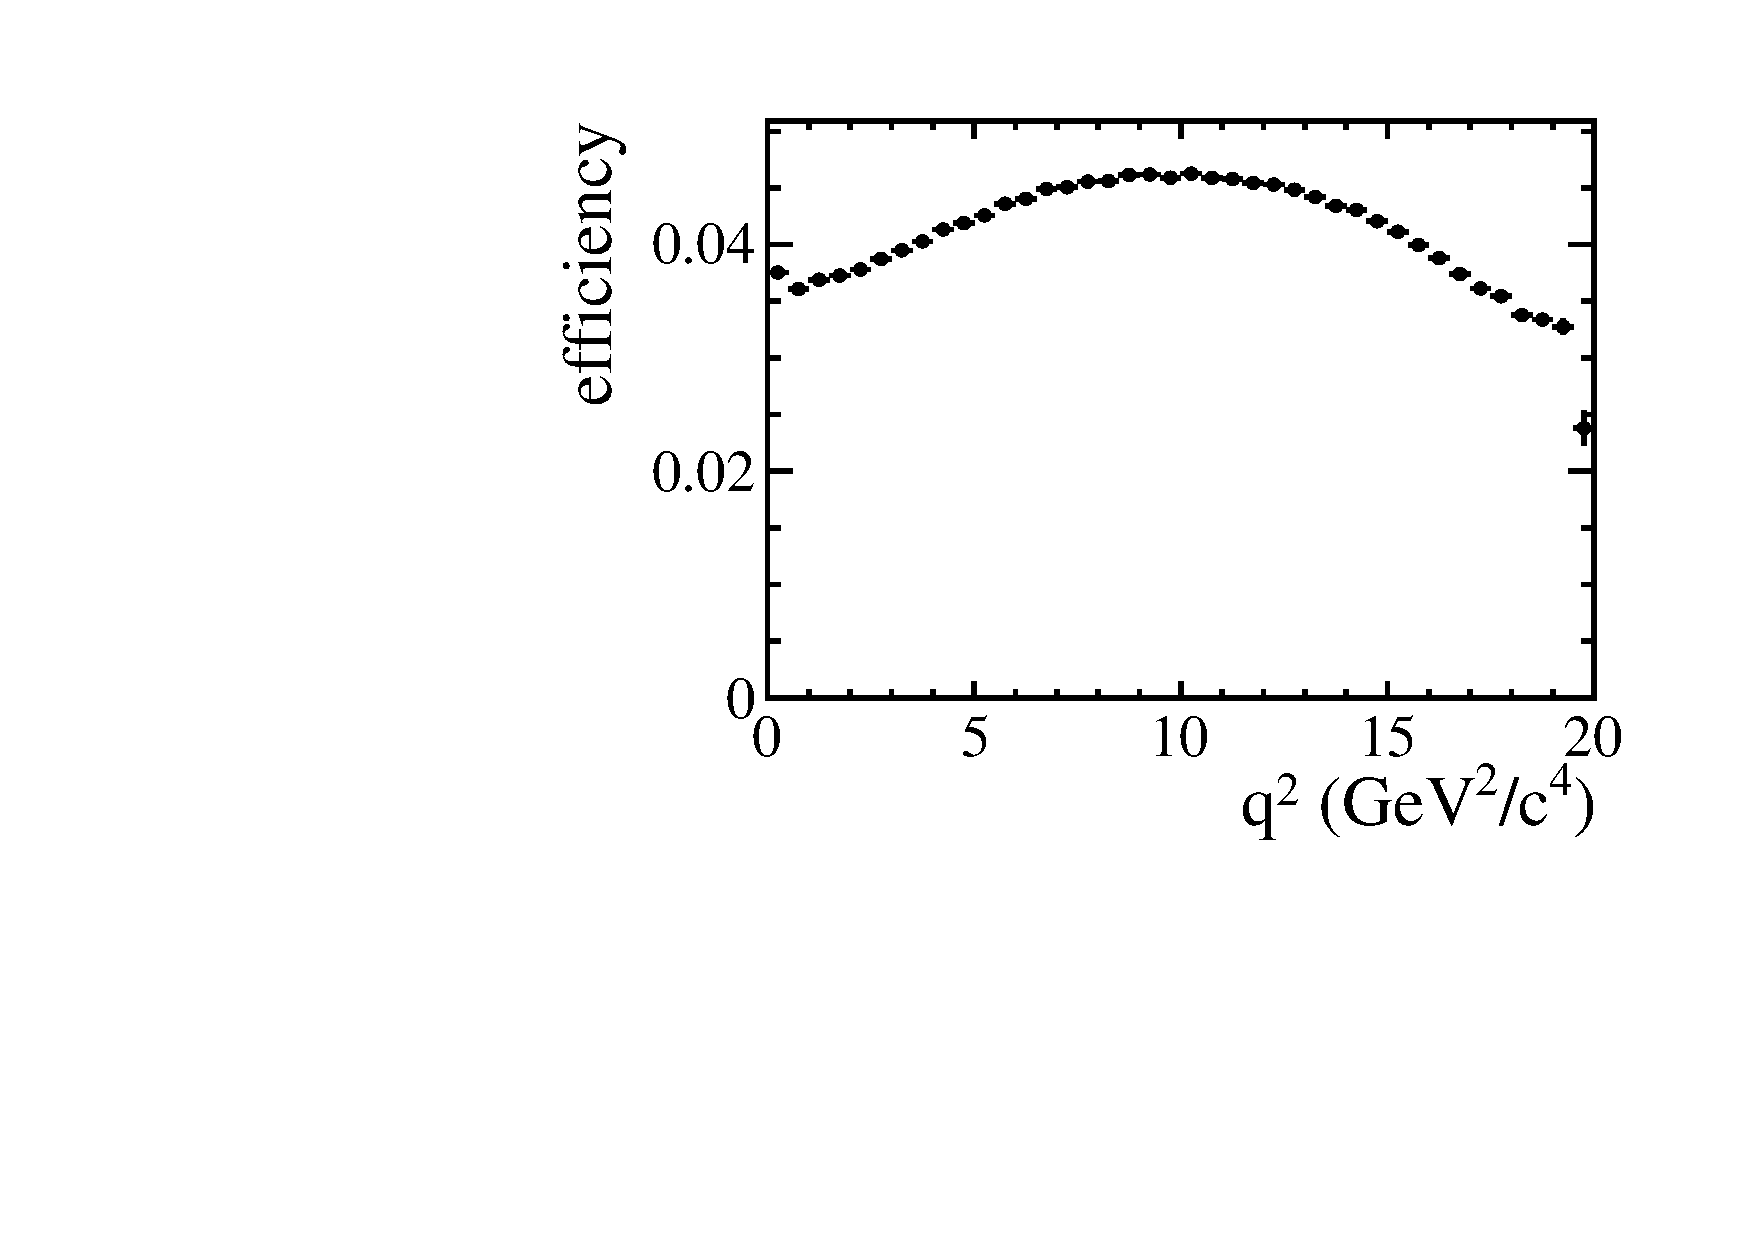
\includegraphics[width=0.48\columnwidth]{chapter5/figs/phsp_qsq_eff_dist.pdf}}
\subfigure[]{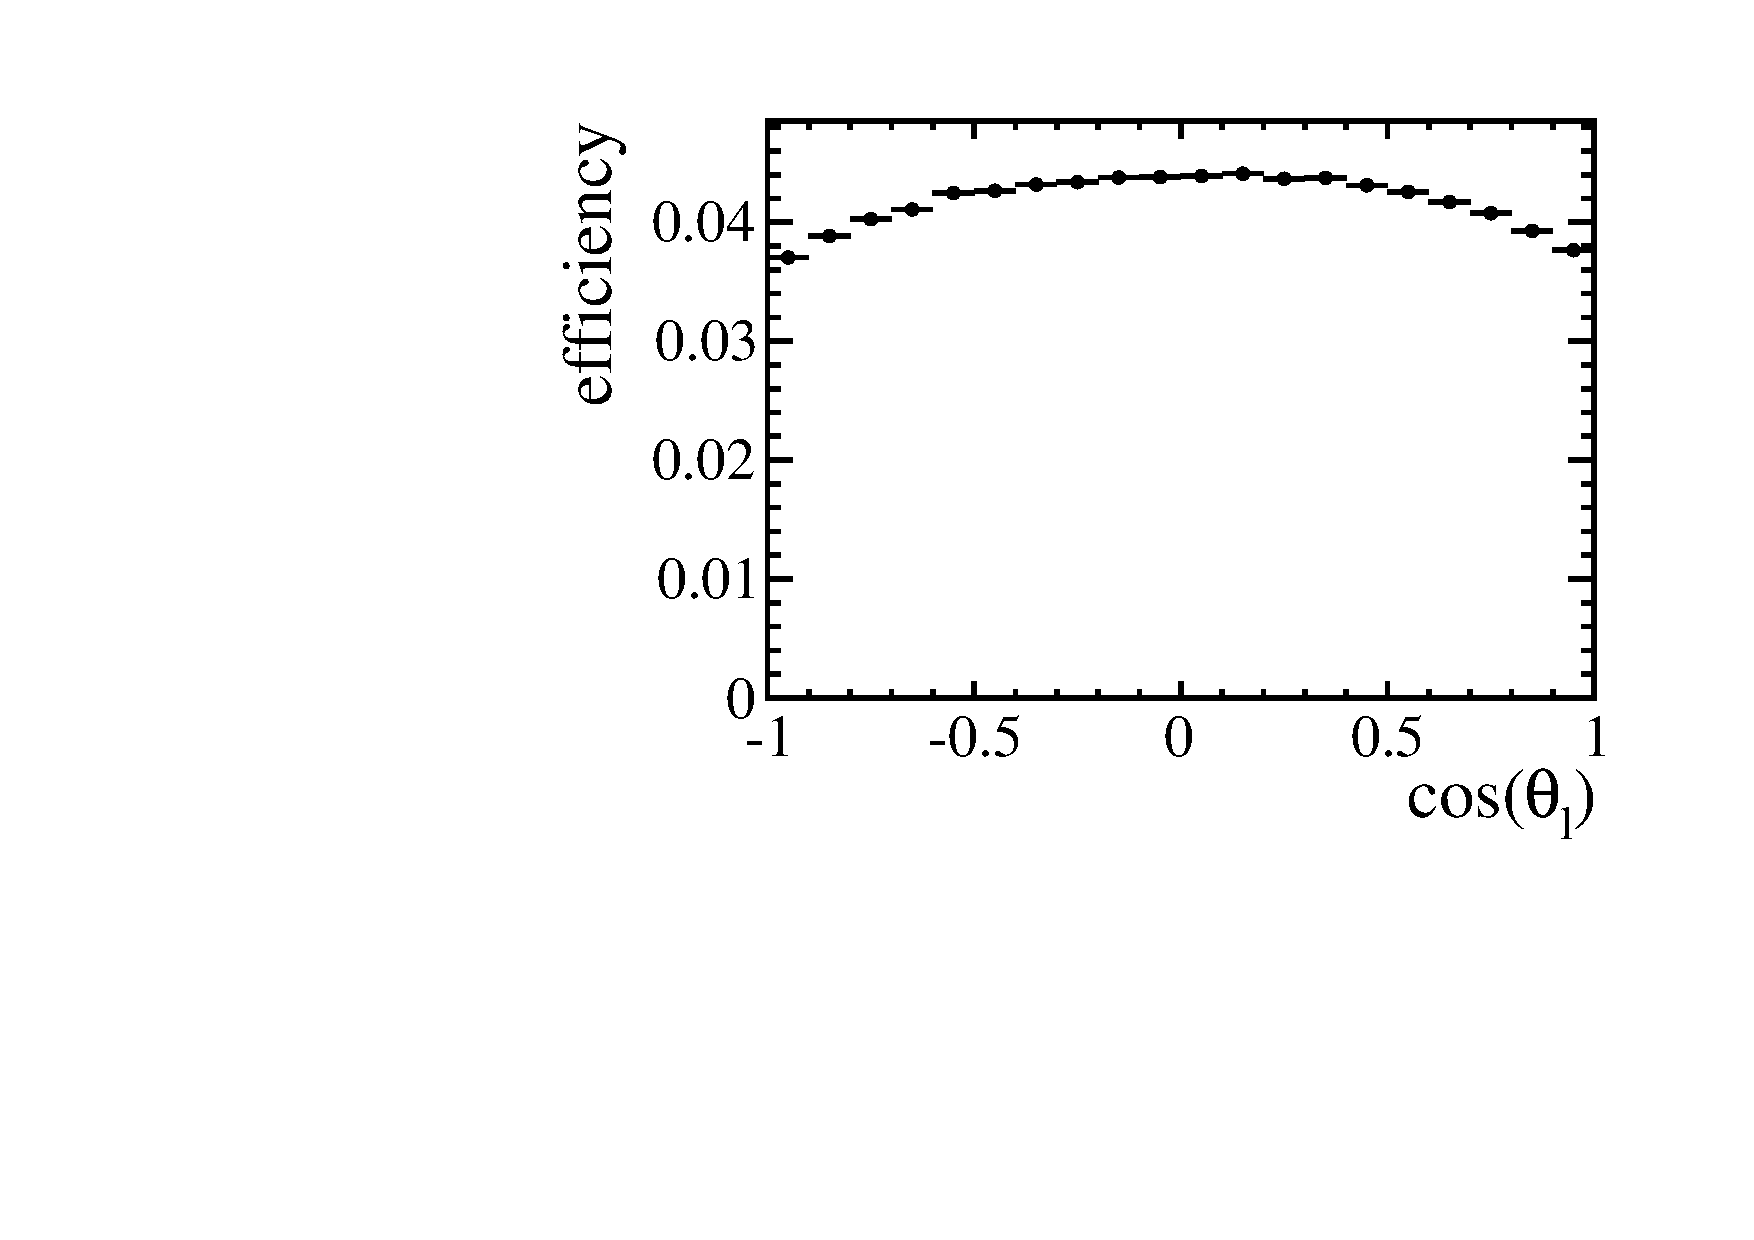
\includegraphics[width=0.48\columnwidth]{chapter5/figs/phsp_ctl_eff_dist.pdf}}
\subfigure[]{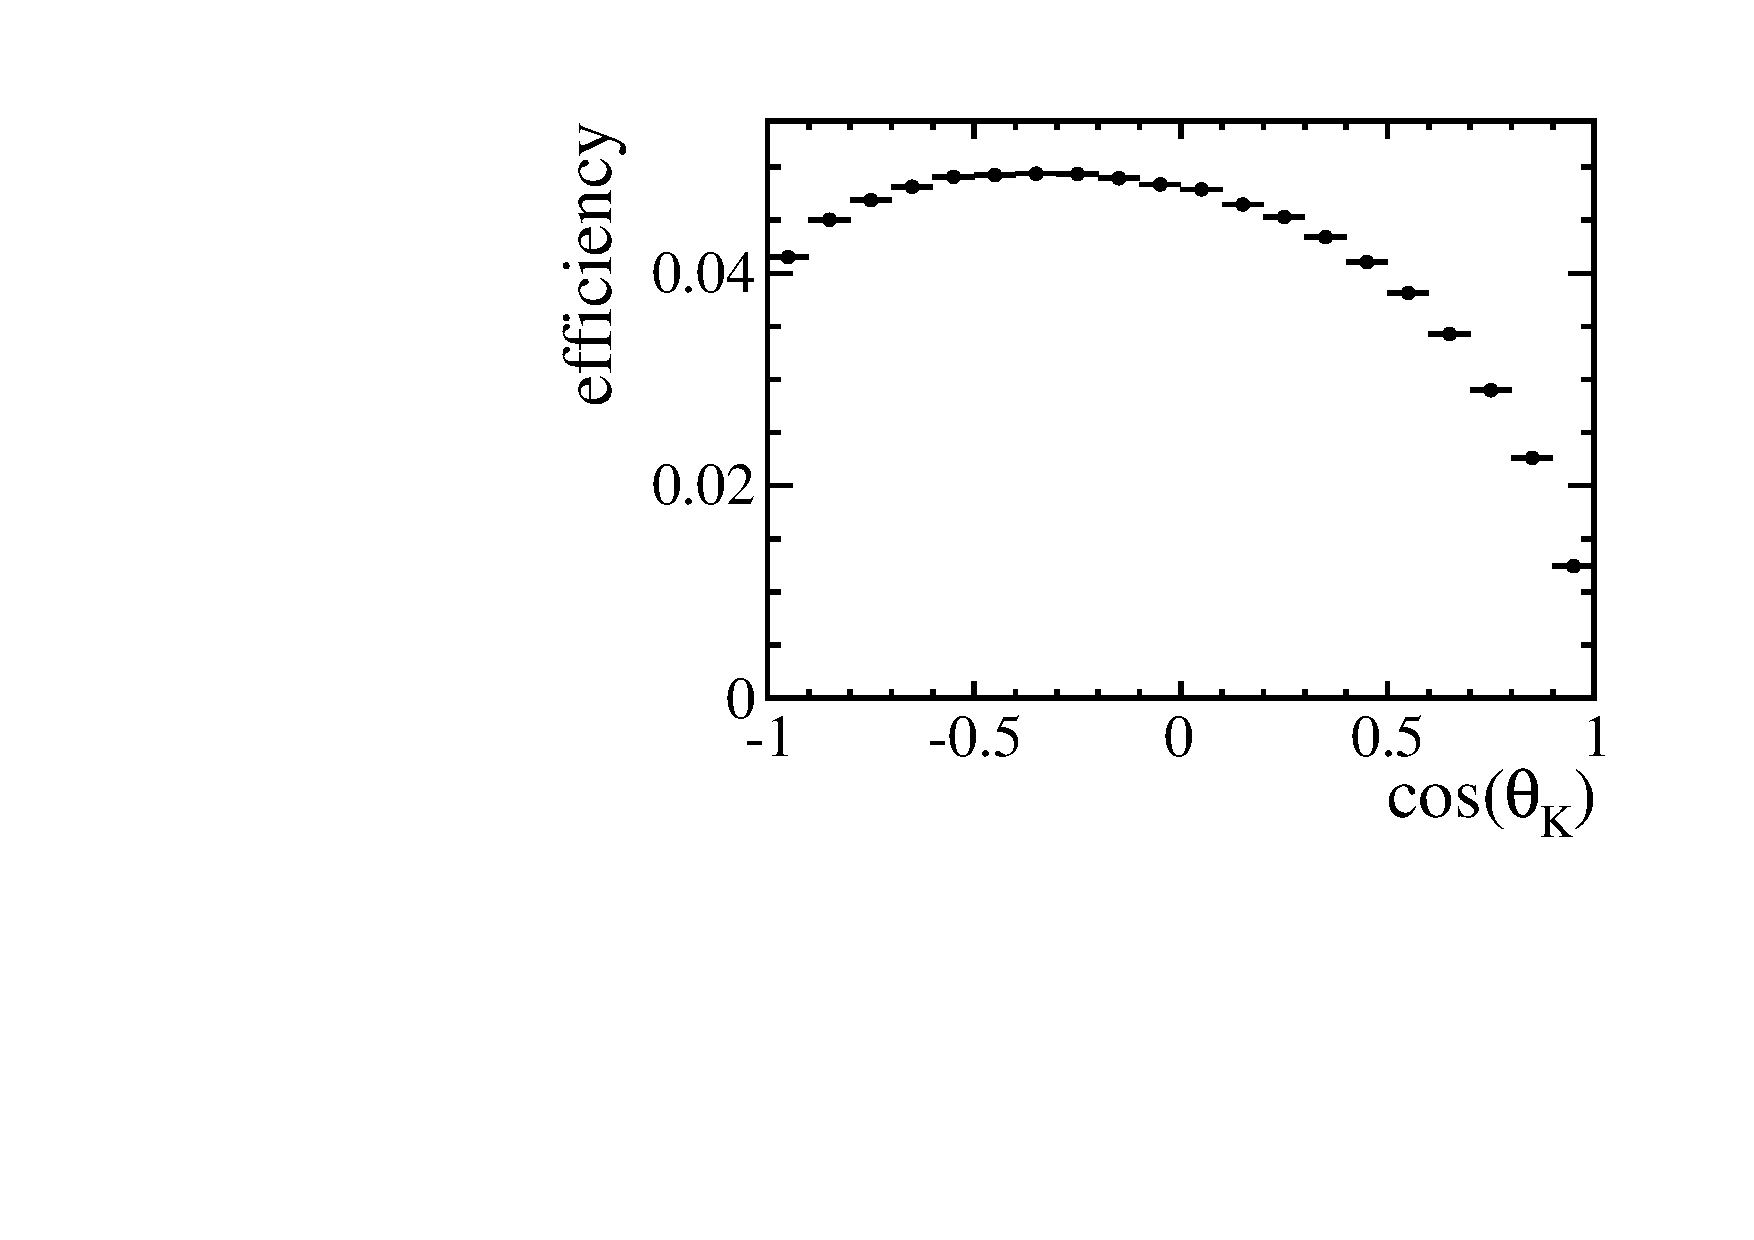
\includegraphics[width=0.48\columnwidth]{chapter5/figs/phsp_ctk_eff_dist.pdf}}
\subfigure[]{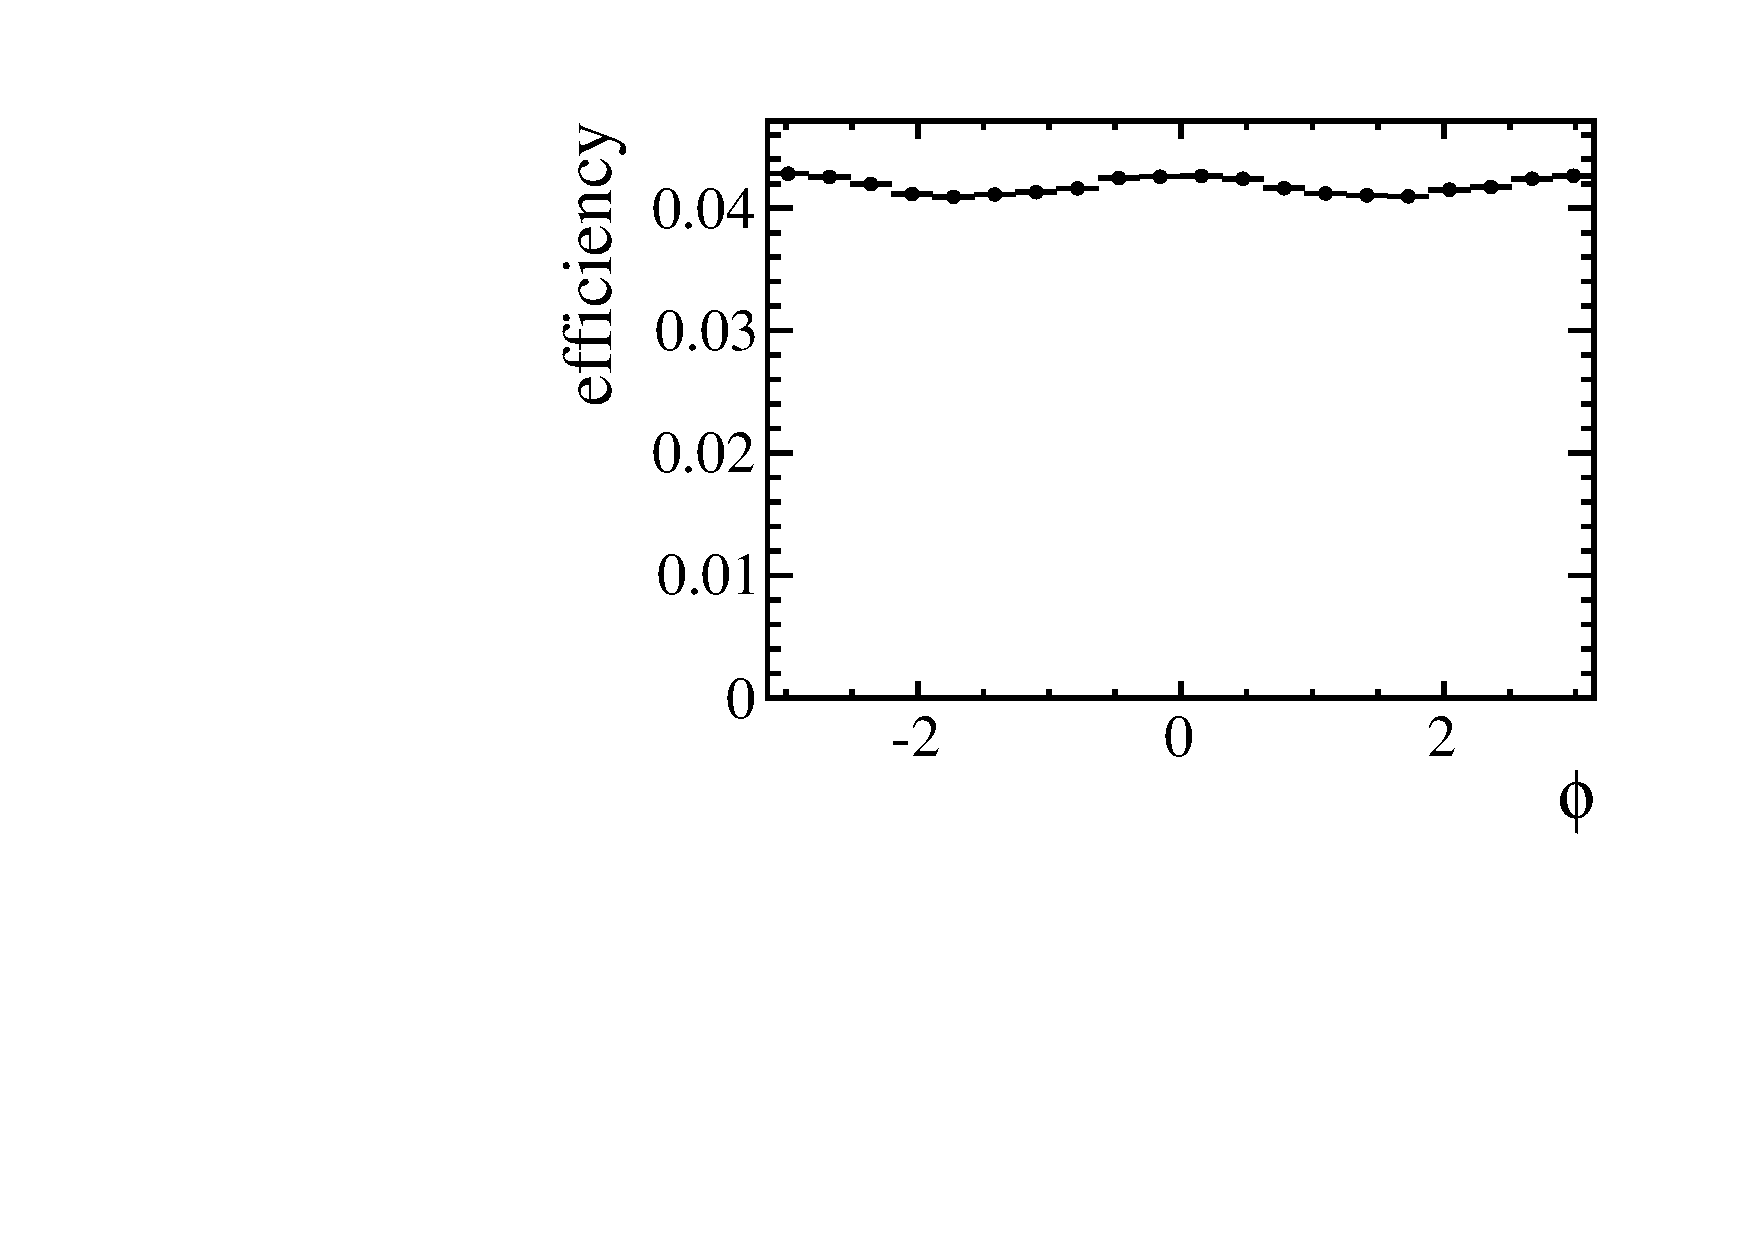
\includegraphics[width=0.48\columnwidth]{chapter5/figs/phsp_phi_eff_dist.pdf}}
\caption[The selection efficiency for \BdToKstmm on simulation]
{The efficiency for selected phase space simulated \BdToKstmm candidates as a function of (a) \qsq, (b) \ctl, (c) \ctk and (d) $\phi$. 
There is a reasonably symmetric acceptance in \ctl and an asymmetric acceptance effect in \ctk. 
The acceptance in \qsq varies across the full range and there is a very small acceptance effect in $\phi$.
 ~\label{fig:phspeff}}
\end{figure}
Is is possible to see the symmetric acceptance at high \ctl, due to 'backward-going' muons in the rest frame of the \Bd that have a very low momenta in the lab frame.
There is an asymmetric acceptance for \ctk from the same effect but the asymmetry is due to the difference in masses of the \kaon and the \pion. 
The different momentum spectra for the kaon and the pion is also affected by both the tracking efficiency and by the particle identification efficiency.
This is where most of the data/simulation corrections have a significant effect.

The total acceptance effect for a four-body decay is a function of the kinematic angles and invariant masses of the di-muon pair and the \kpi pair. 
The \psq window is assumed to be sufficiently small that there is no varying acceptance effect within it.
The angular analysis is performed in bins of \qsq requiring that the acceptance effect is corrected for on a finer level than the \qsq binning.


\subsection{A full 3D acceptance correction algorithm}
\label{sec:kstmm:ac:knnac}

One method of evaluating the efficiency as a function of phase space  is to count events before and after the selection
in fine bins of phase space.
This method was used in the first angular analysis of 0.38\invfb of data.
For an event at a particular point, the efficiency can be calculated by comparing the number of offline selected 
events with the number of generator level events `close' to that point : 
\begin{align}
\epsilon (\ctl, \ctk, q^2)_{r<R} = \frac{\offsel~(\delta d < R)  }{\genlvl~(\delta d < R)  } = \frac{n}{m}
\label{eq:eff}	
\end{align}
where $n$ is the number of weighted offline selected simulated events and $m$ is the number of generator level simulated events.
The distance $d$ is defined over the metric of the phase space and $R$ is the maximum distance within which events are chosen to contribute 
to the efficiency calculation.
The condition $\delta d < R$ defines a hyper-spheroid over the phase space.
The distance between event $i$ and event $j$, $\delta d_{ij}$, is given by
\begin{align}
\delta d_{ij} = \frac{1}{N_{\ctl}}( \ctl_i - \ctl_j  )^2 + \frac{1}{N_{\ctk}}( \ctk_i - \ctk_j) ^2 + \frac{1}{N_{\qsq}}( \qsq_i - \qsq_j) ^2 
\label{eq:distance}
\end{align}
where the normalisation factors, $(N_{\ctl}, N_{\ctk},N_{\qsq})$, are chosen such that the dimensions are each scaled between $[0,1]$. 
In order to collect events efficiently, a $k$-nearest neighbour algorithm was used to collect events in a small region of phase space. 

The error on the efficiency for a given bin is defined by the combination of the Poisson errors from $n$ and $m$, i.e.
\begin{align}
\sigma_{\epsilon} = \epsilon \times \sqrt{\frac{\sigma_n^2}{n^2} + \frac{1}{m}},
\end{align}
since the offline selection simulation is not a subset of the generation simulation.
The maximum radius $R$ is chosen such that the statistical error from the number of events within the hyper-spheroid is sufficiently small when compared to the size of the phase space. 
The average error and the average fractional error as a function of the radius of the hyper-spheroid is shown in Fig.~\ref{fig:errorvsradii}.
\begin{figure}[tbp]
\centering
\subfigure[]{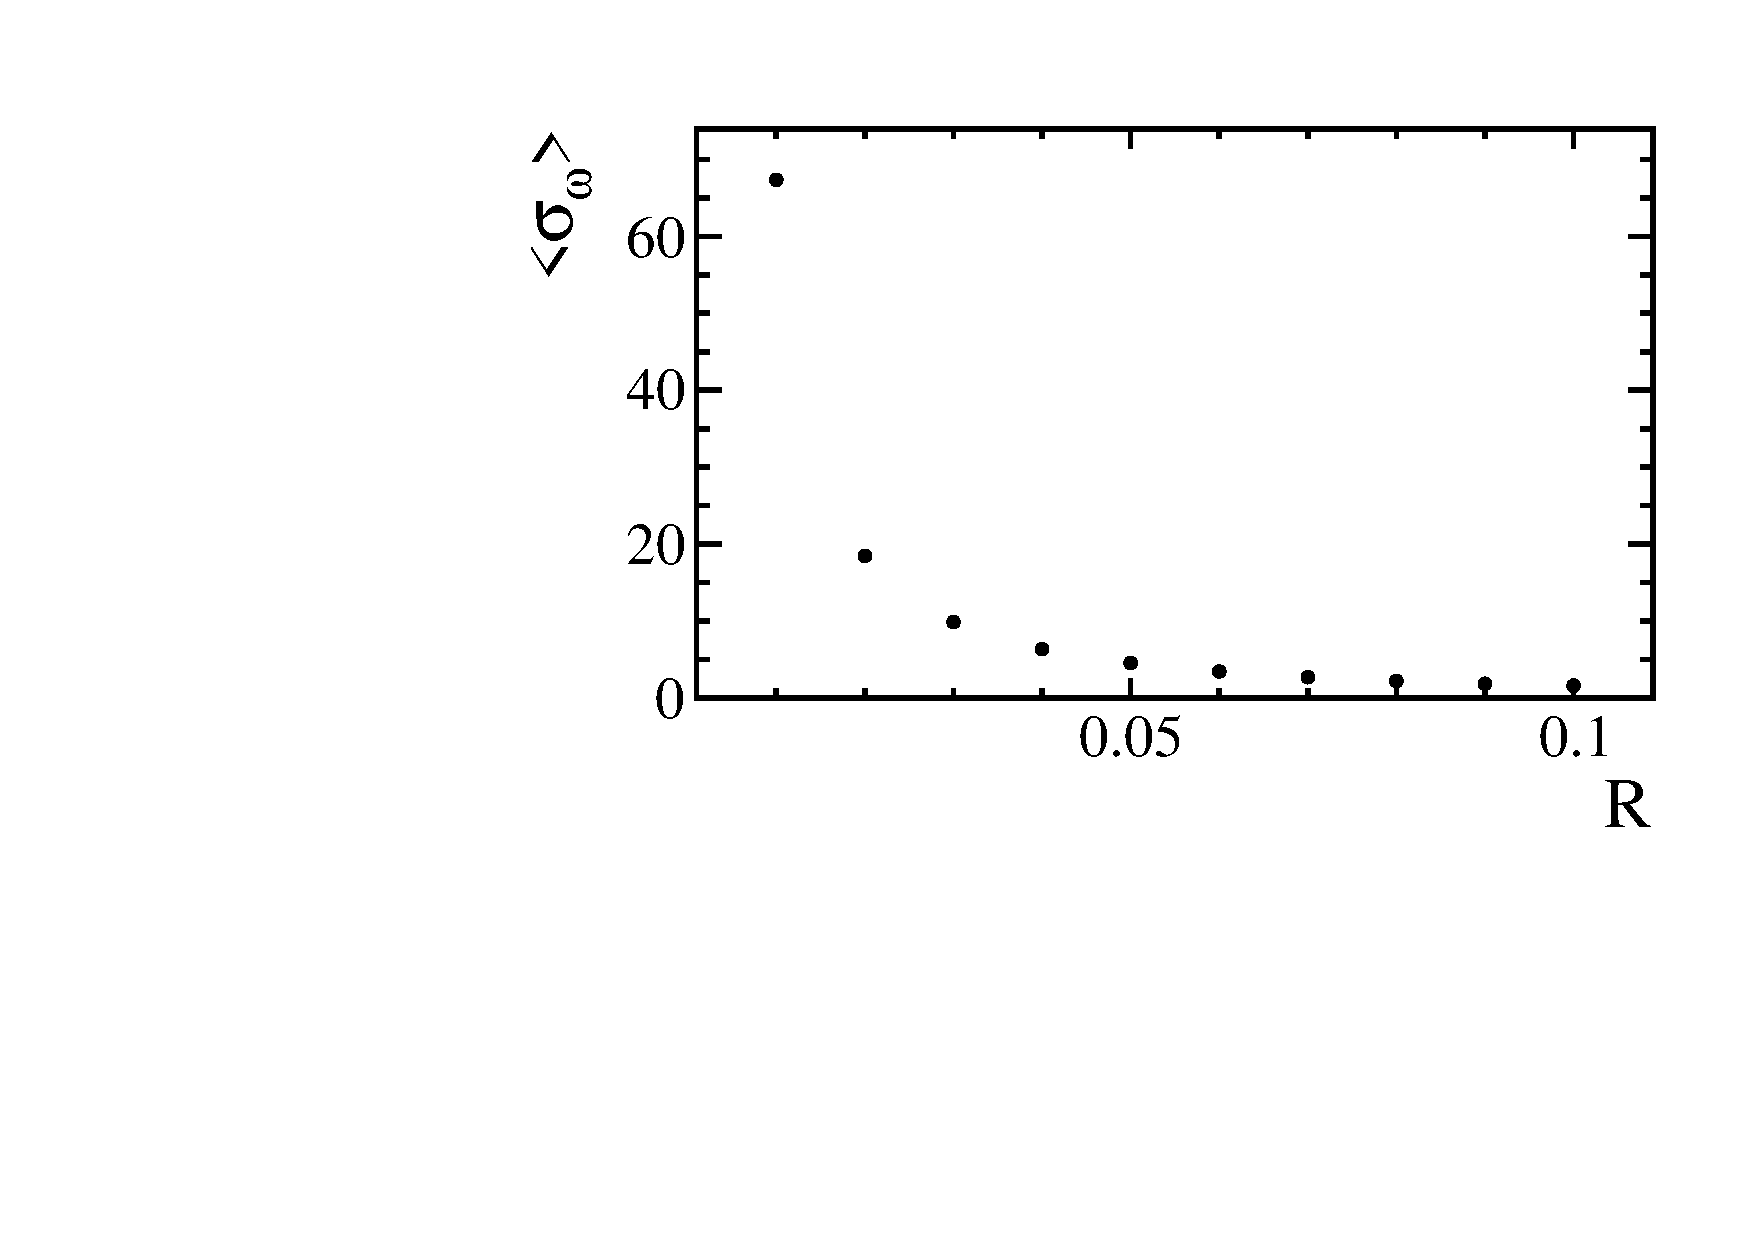
\includegraphics[width=0.48\columnwidth]{chapter5/figs/ac1/error_vs_radius.pdf}}
\subfigure[]{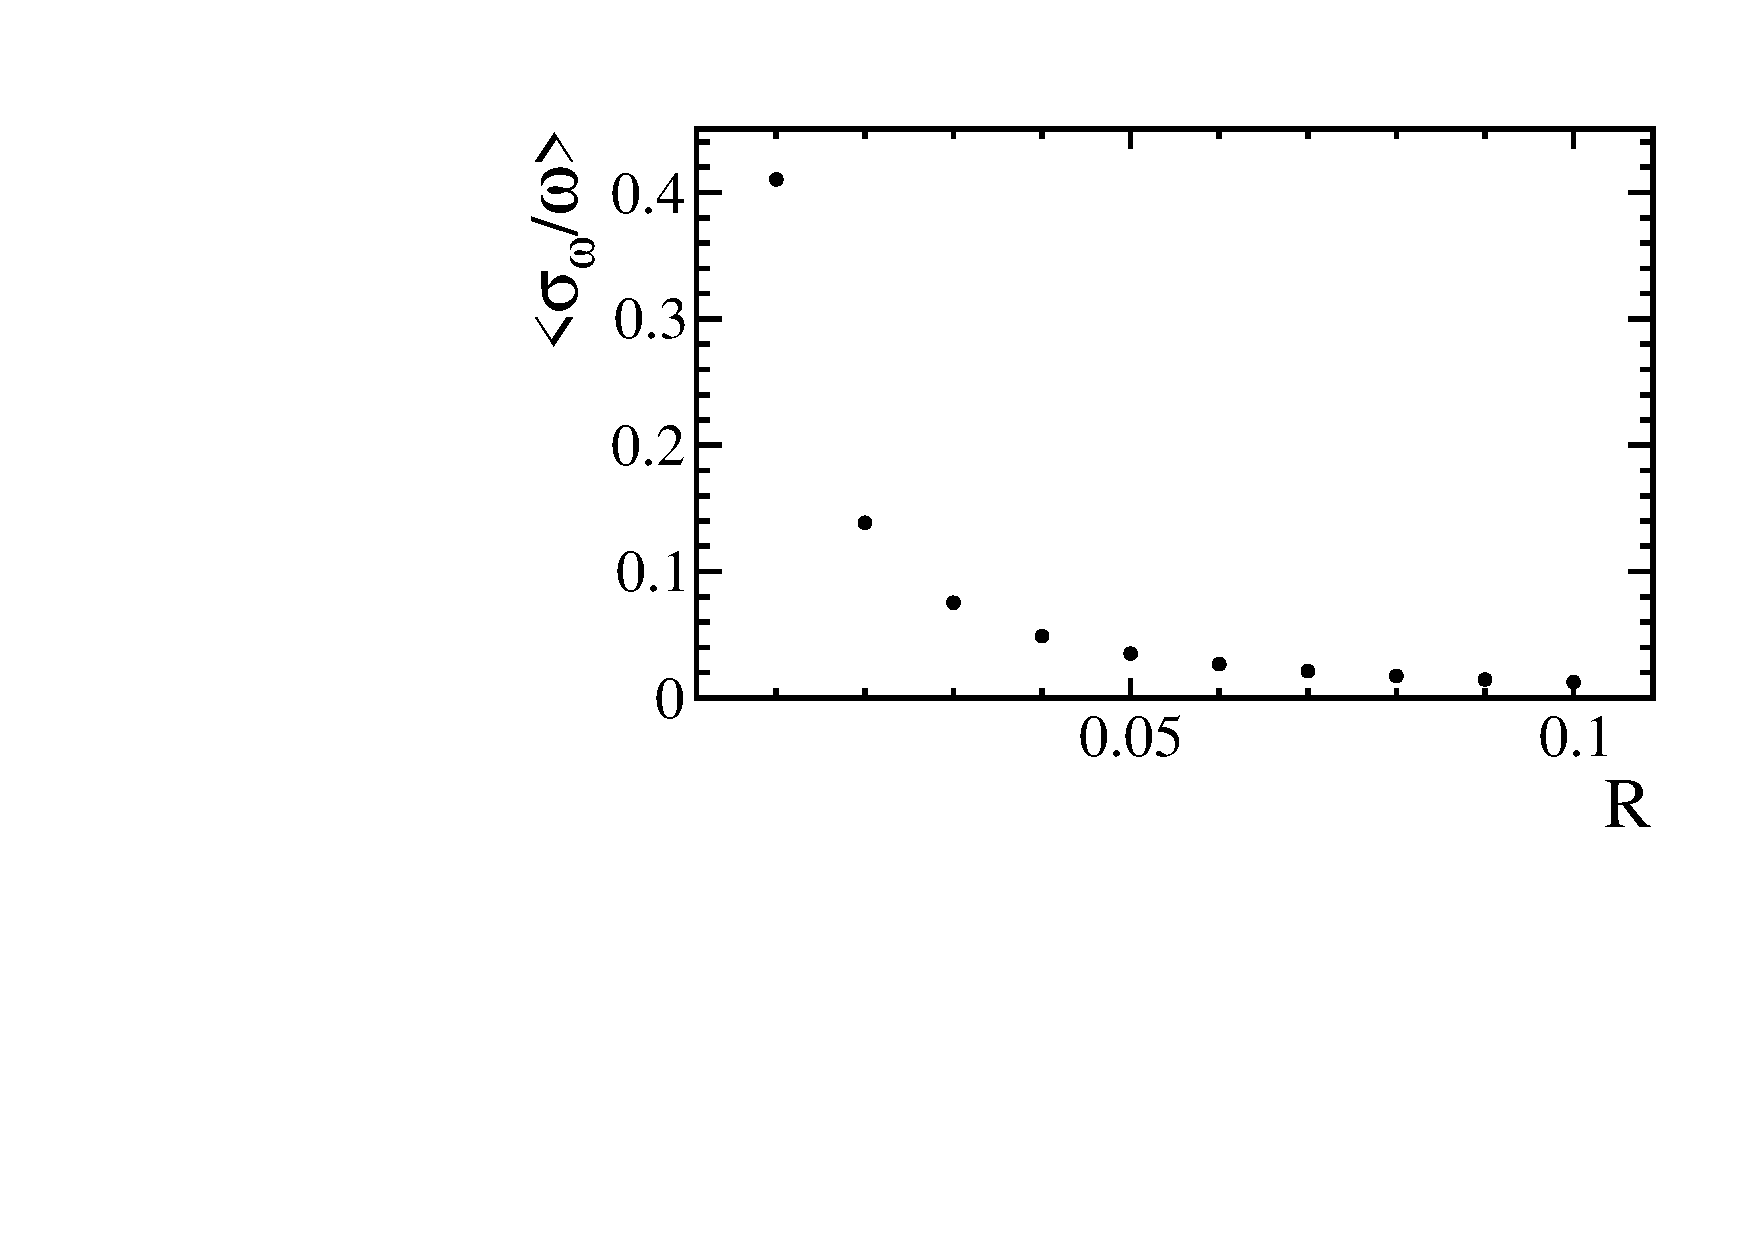
\includegraphics[width=0.48\columnwidth]{chapter5/figs/ac1/prop_error_vs_radius.pdf}}
\caption[The error on the acceptance correction weights.]
{ The average error (a) and the fractional error (b) on 150 weights for \BdToKstmm phase space simulated events for radii between 0.01 and 0.1. 
It is possible to see the $\sqrt{n^3}$ behaviour in the reduction of the error as more events are used to calculate the efficiency.
 ~\label{fig:errorvsradii} }
\end{figure}
The average error follows the expected Poisson behaviour but the fractional error is significant for radii of less than 0.02.

For the first angular analysis of 0.38\invfb of data, a radius of $R = 0.02$ was used to calculate an acceptance correction weight on an event-by-event basis.
This is chosen as a balance between contributing a large systematic error and retaining the accuracy on the correction.
The distribution of acceptance correction weights on data and the 
correlation between these weights and the angles are shown in Fig.~\ref{fig:ac1weights}.
\begin{figure}[tbp]
\centering
\subfigure[]{\includegraphics[width=0.48\columnwidth]{chapter5/figs/ac1/phasespace_weight_value.pdf}}
\subfigure[]{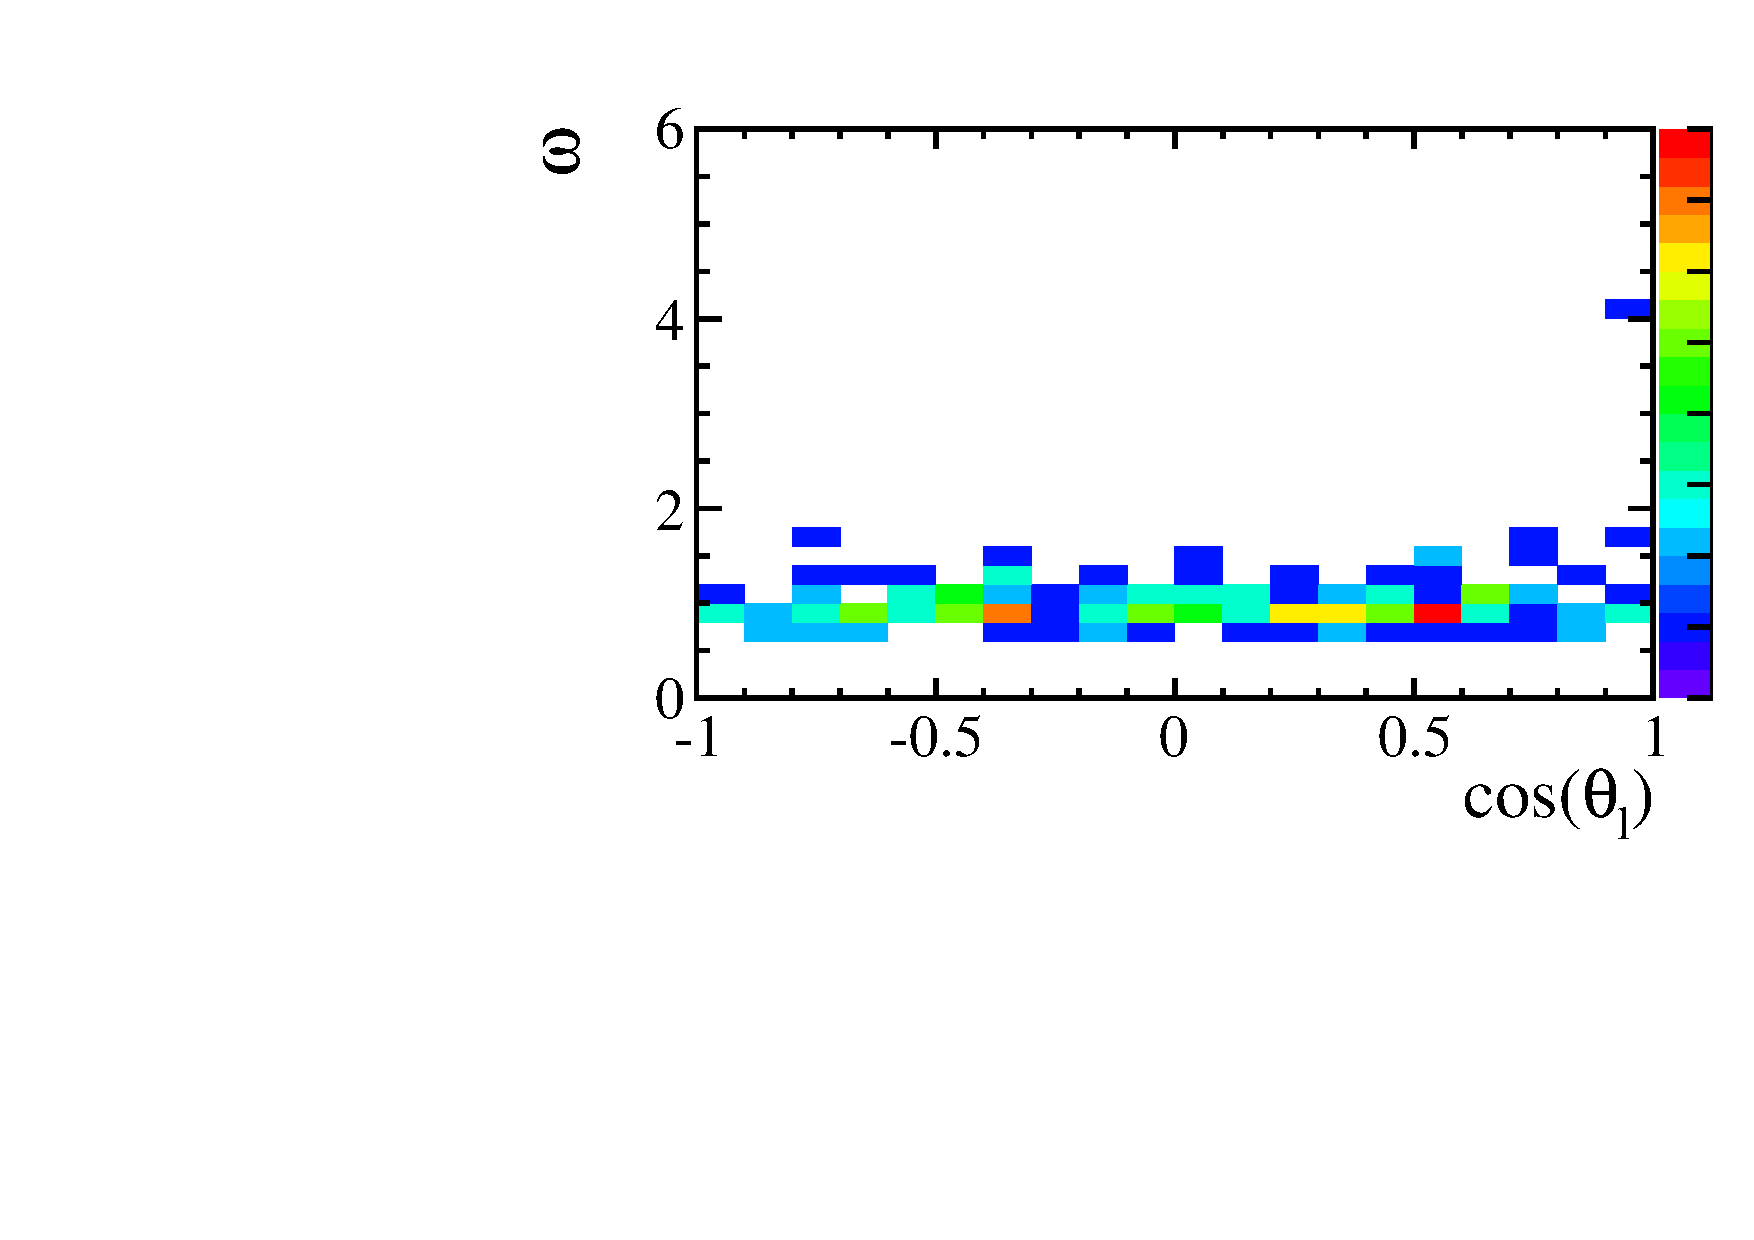
\includegraphics[width=0.48\columnwidth]{chapter5/figs/ac1/phasespace_weight_ctl.pdf}}
\subfigure[]{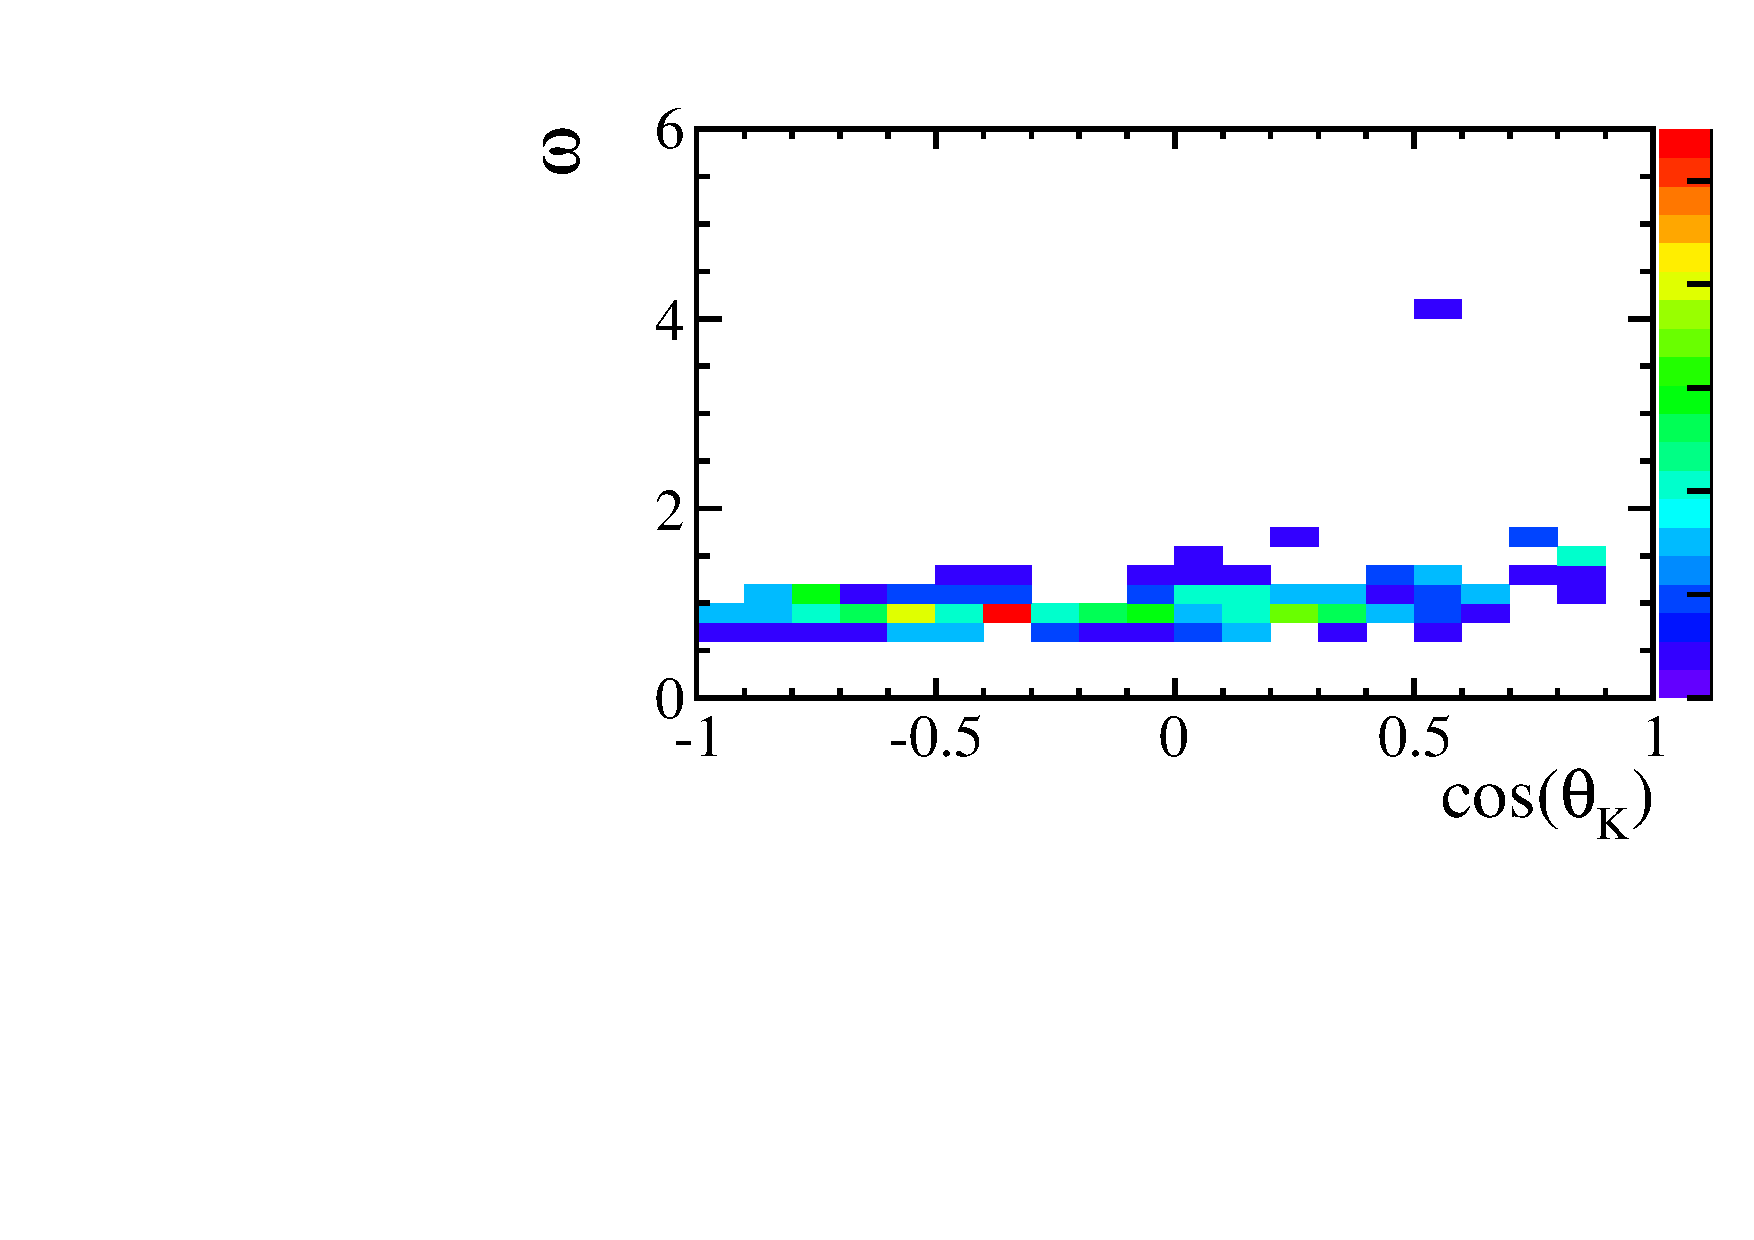
\includegraphics[width=0.48\columnwidth]{chapter5/figs/ac1/phasespace_weight_ctk.pdf}}
\caption[The weight distribution of acceptance corrected \BdToKstmm data.]
{ The distribution of weights for 150 phase space simulated \BdToKstmm events (a) and the correlation between 
the weights and \ctl (b) and \ctk (c). The weights are normalised such that the sum of weights is equal to the 
number of events. The high weights for extreme \ctk and \ctl can be seen. ~\label{fig:ac1weights} }
\end{figure}
It is possible to see that the weight values at extreme ($|\ctk|>0.8$) \ctk are higher than the weights in the centre.
The same effect can be seen in \ctl but to a lesser degree due to the integration over \qsq.
However, at low and high \qsq it is possible to see a variation of weights to accommodate the change in acceptance.

One limitation of the $k$-nearest-neighbour algorithm is 
that the error on the efficiency is entirely dominated 
by the number of offline selected simulated events at high \qsq.
If the data sample is binned more finely than the chosen collection radius $R$,
 then the `averaging effect' over the hyper-spheroid can be seen. 
In Fig.~\ref{fig:jpsikstardodgy}, an example of this can be seen in the large \BdToJpsiKstar sample.
\begin{figure}[tbp]
\centering
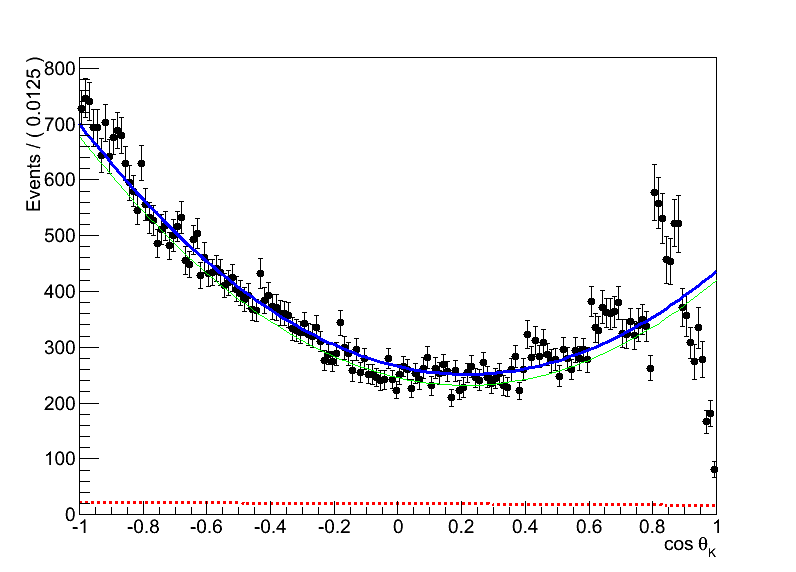
\includegraphics[width=0.48\columnwidth]{chapter5/figs/acceptance_variation_overbin.png}
\caption[ Weighted \BdToJpsiKstar events using a radius of $R = 0.05$. ]
{ Weighted \BdToJpsiKstar events using a radius of $R = 0.05$. 
The total expected number of events is shown in blue, along with the total expected number of signal events in green and the number of background events in red.
The effect of integrating over a rapidly varying efficiency is 
evident at high \ctk with a large statistics data sample. ~\label{fig:jpsikstardodgy} }
\end{figure}
A second limitation of the $k$-nearest-neighbour algorithm is the computational performance. 
The algorithm is at worst of order $\mathcal{O}(n)$ per event.
This can be simplified by only searching for neighbours in a small region of phase 
space, sufficient to encompass the subset of events within the radius $R$. 
As the number of events in the simulation has to scale with the size of the data, $n_{data}$,
 the overall scaling of the algorithm is $\mathcal{O}(n_{data}^2)$.
This, along with the required decrease in the systematic uncertainty on the efficiency calculation, 
necessitated the development of a more 
efficient acceptance algorithm for the angular analysis on the full 2011 dataset.

\subsection{A factorised acceptance correction algorithm}
\label{sec:kstmm:ac:facac}

In order to reduce the error on the acceptance correction beyond the reduction in statistical error for the full 2011 dataset, a factor of $1/\sqrt{3}$ was required to compensate for the threefold increase in data.
One solution to this issue, along with reducing the $\mathcal{O}(m^2)$ scaling of the $k$-nearest neighbour algorithm, 
is to model the distribution of events before and after selection using a \PDF.
The error on the fitted PDFs at a point in phase space is smaller than the error on a bin of $k$ events because 
the whole dataset is used to evaluate the efficiency.
%and PDFs, once fitted, can be evaluated at each point in phase space quickly.

In general, the efficiency function is not analytical so the choice of PDF to model the efficiency is entirely empirical.
The efficiency can be calculated at a particular point in phase space,
\begin{align}
\epsilon(\ctl, \ctk, \phi, \qsq) = \frac{n}{m} \times \frac{ S( \ctl, \ctk, \phi, \qsq ) }{ G( \ctl, \ctk, \phi, \qsq )  }  \, ,
\end{align}
where $S$ is the \PDF modelling the selected data and $G$ is the \PDF modelling the generator level data.
 The PDFs are normalised by the weighted number of events in the selected sample ($n$) divided by the number of generator level events ($m$).

Maximum use of the simulated events to give a large reduction in the error can be made by factorising the efficiency in the form,
\begin{align}
\epsilon(\ctl, \ctk, \phi,\qsq)  = \epsilon(\ctl)\times\epsilon(\ctk)\times\epsilon(\phi)\times\epsilon(\qsq) \, .
\end{align}
This factorisation is in general not possible due to the fact that there is a correlation between the angles and \qsq.
The efficiency for each of the angles for offline selected simulated phase space \BdToKstmm events 
 in a low \qsq bin are given in Fig.~\ref{fig:phspeff2d}. 
\begin{figure}[tbp]
\centering
\subfigure[\ctl v.s. \ctk]{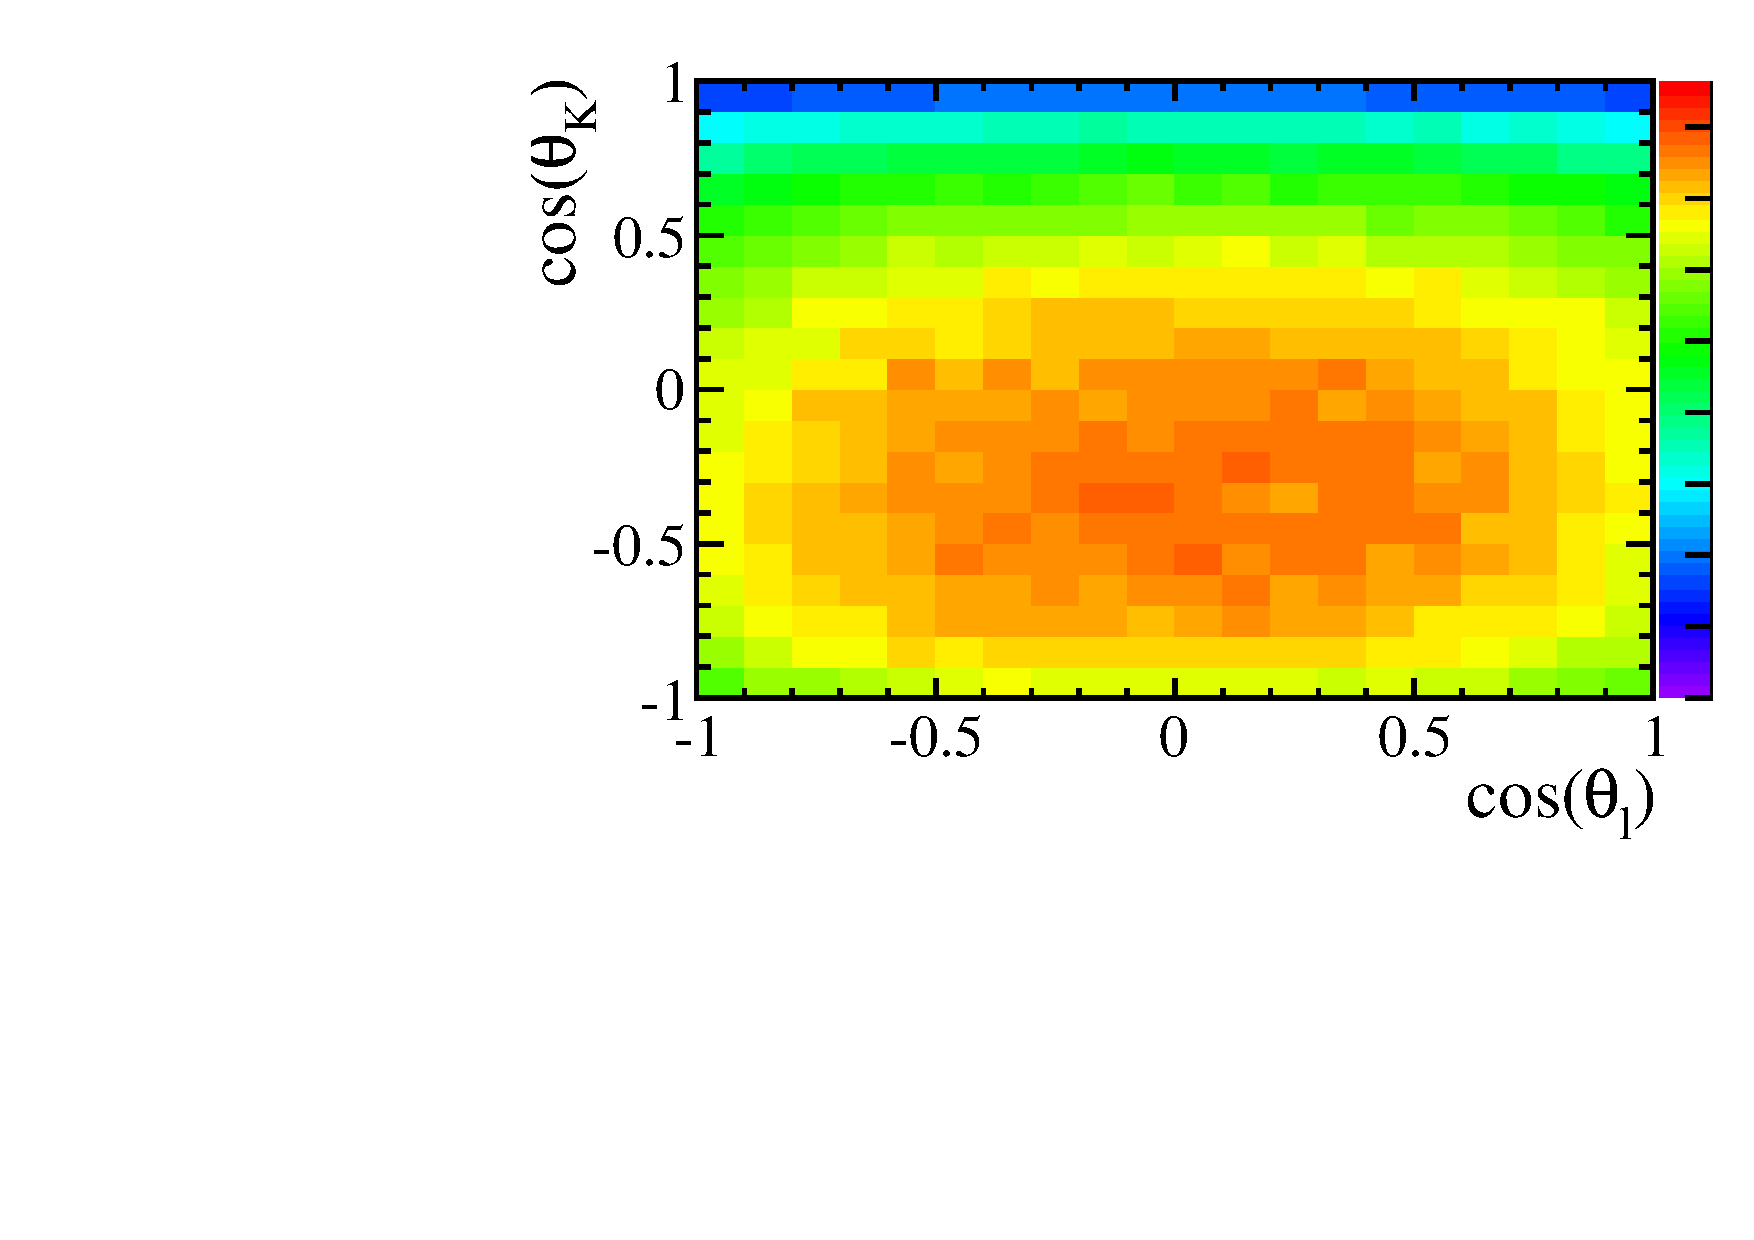
\includegraphics[width=0.48\columnwidth]{chapter5/figs/phsp_ctl_ctk_sel_dist.pdf}}
\subfigure[\ctl v.s. $\phi$]{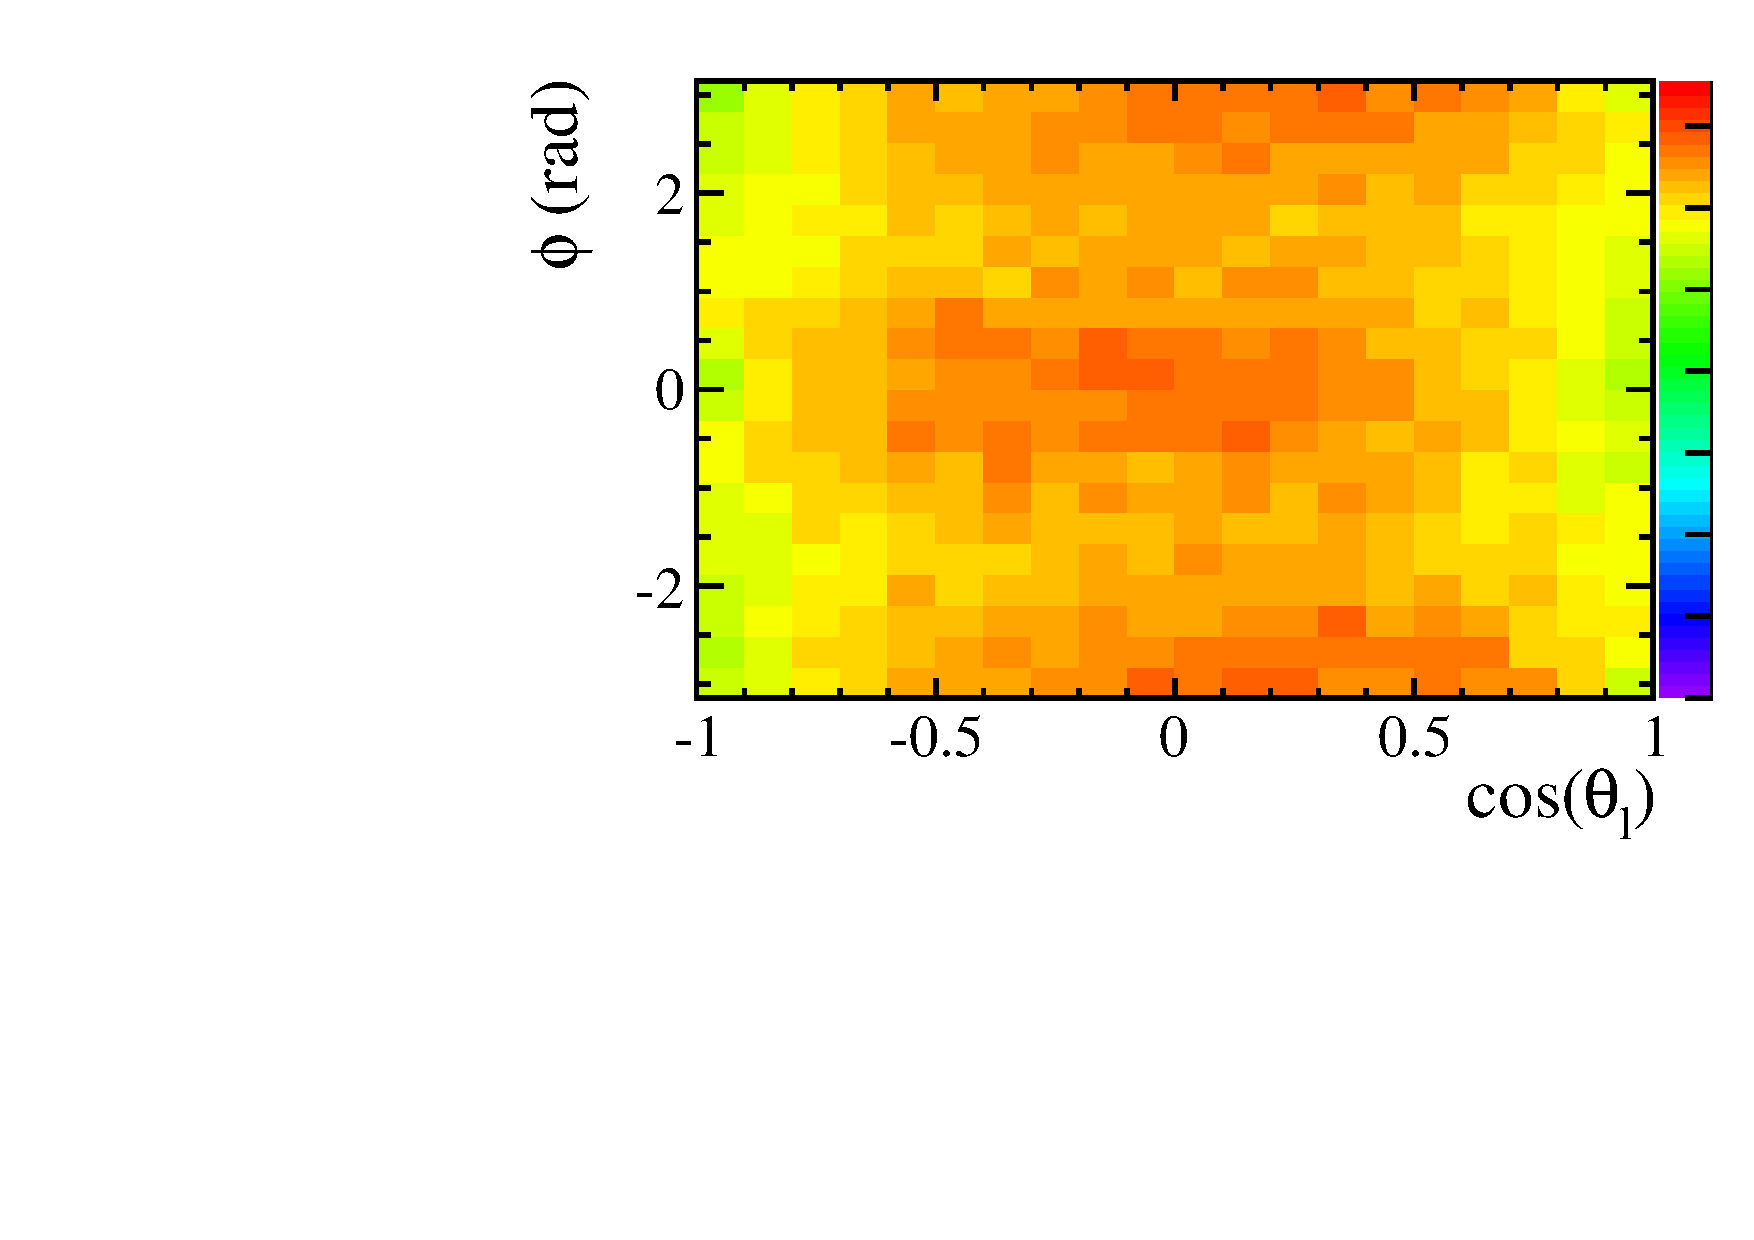
\includegraphics[width=0.48\columnwidth]{chapter5/figs/phsp_ctl_phi_sel_dist.pdf}}
\subfigure[\ctk v.s. $\phi$]{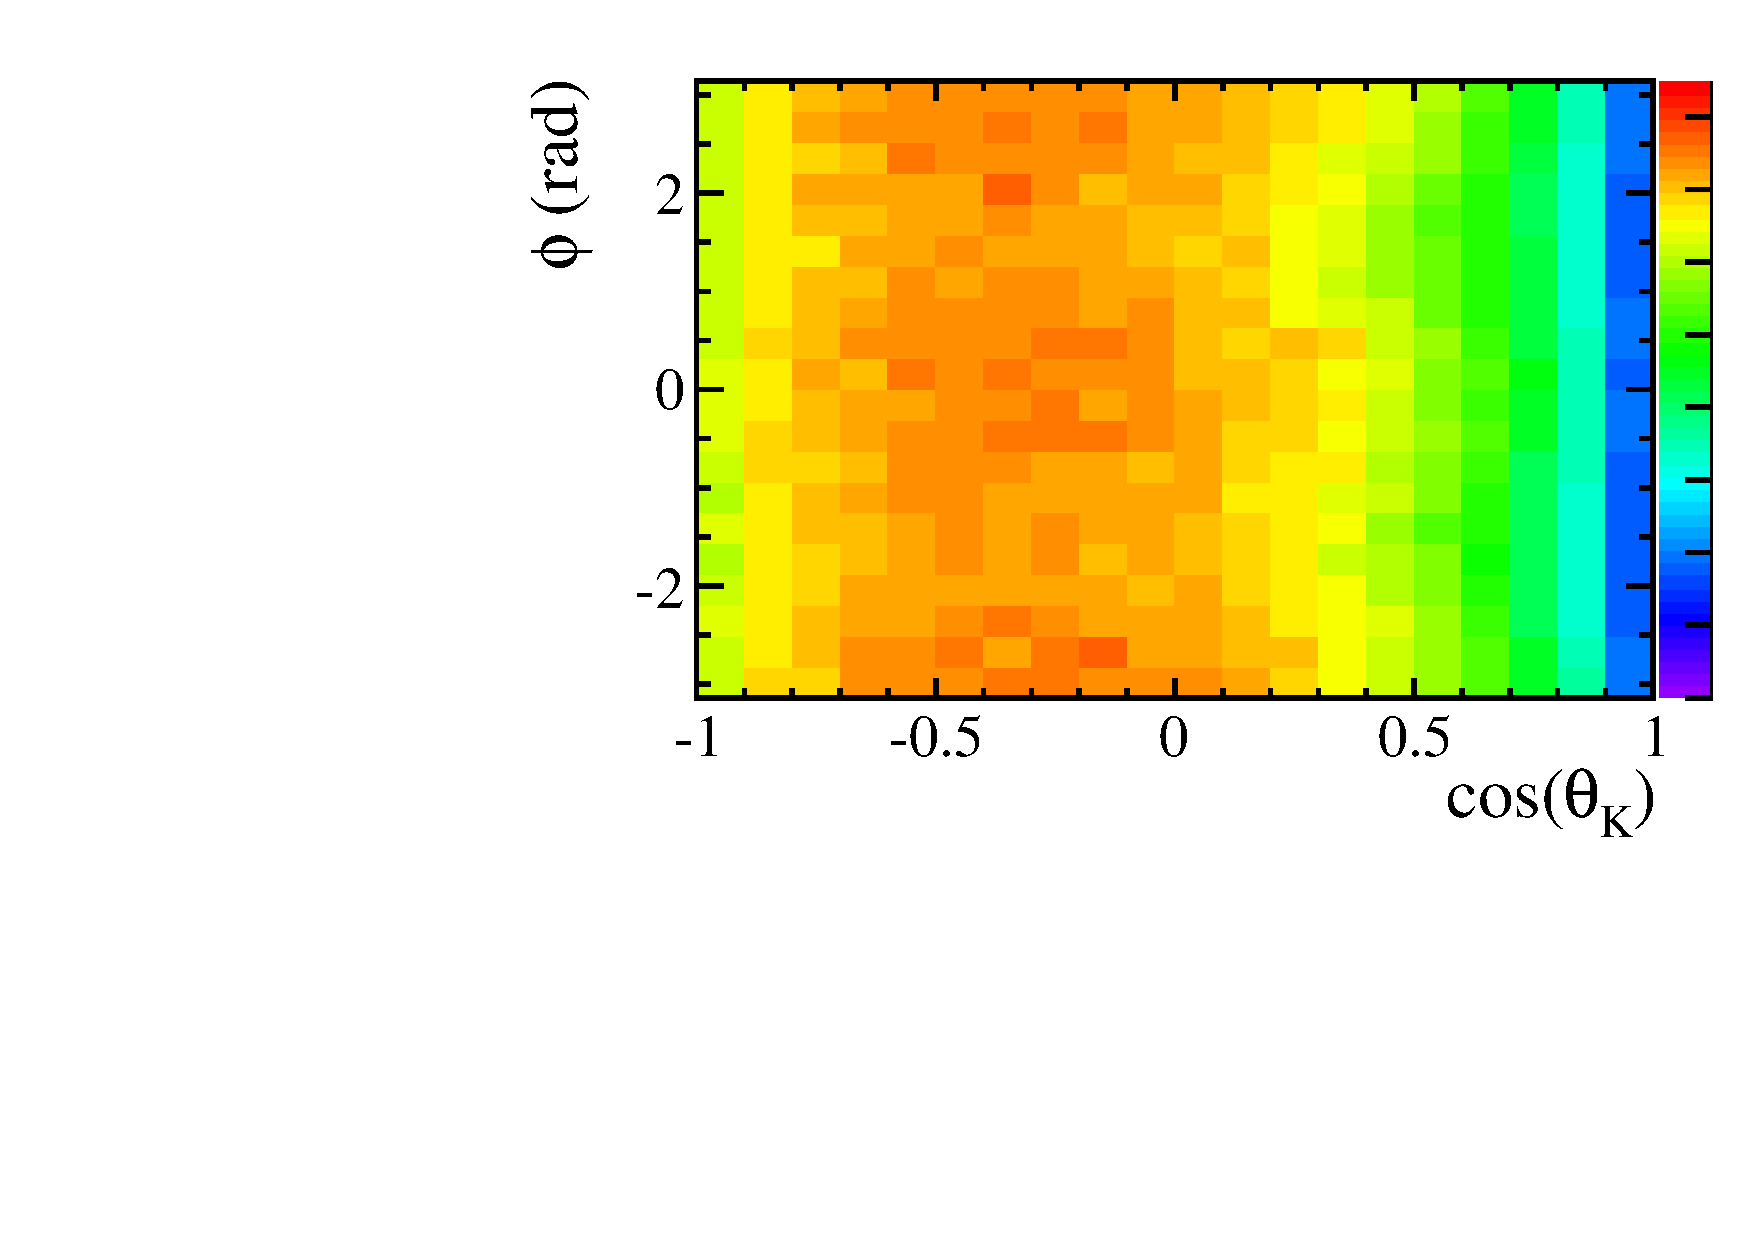
\includegraphics[width=0.48\columnwidth]{chapter5/figs/phsp_ctk_phi_sel_dist.pdf}}
\subfigure[\ctl v.s. \qsq]{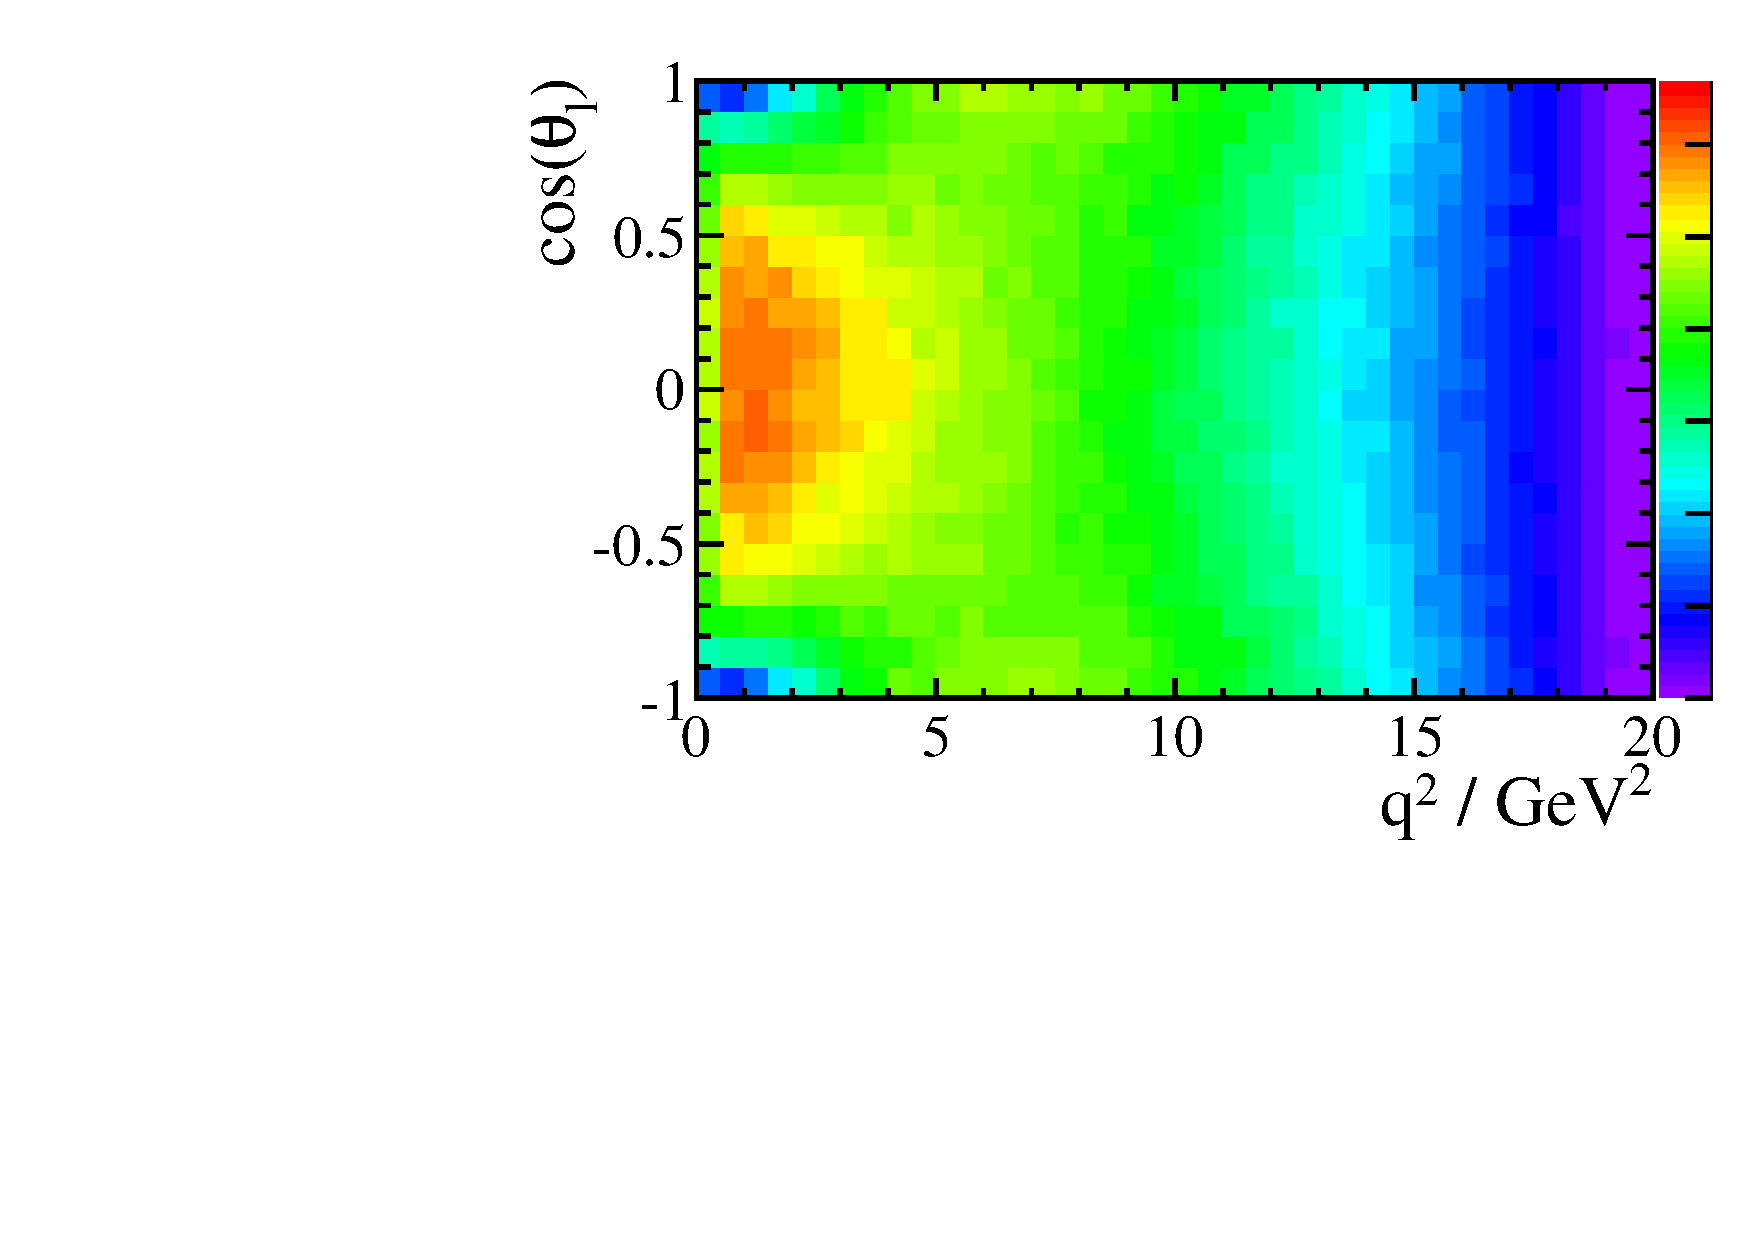
\includegraphics[width=0.48\columnwidth]{chapter5/figs/phsp_ctl_qsq_sel_dist.pdf}}
\subfigure[\ctk v.s. \qsq]{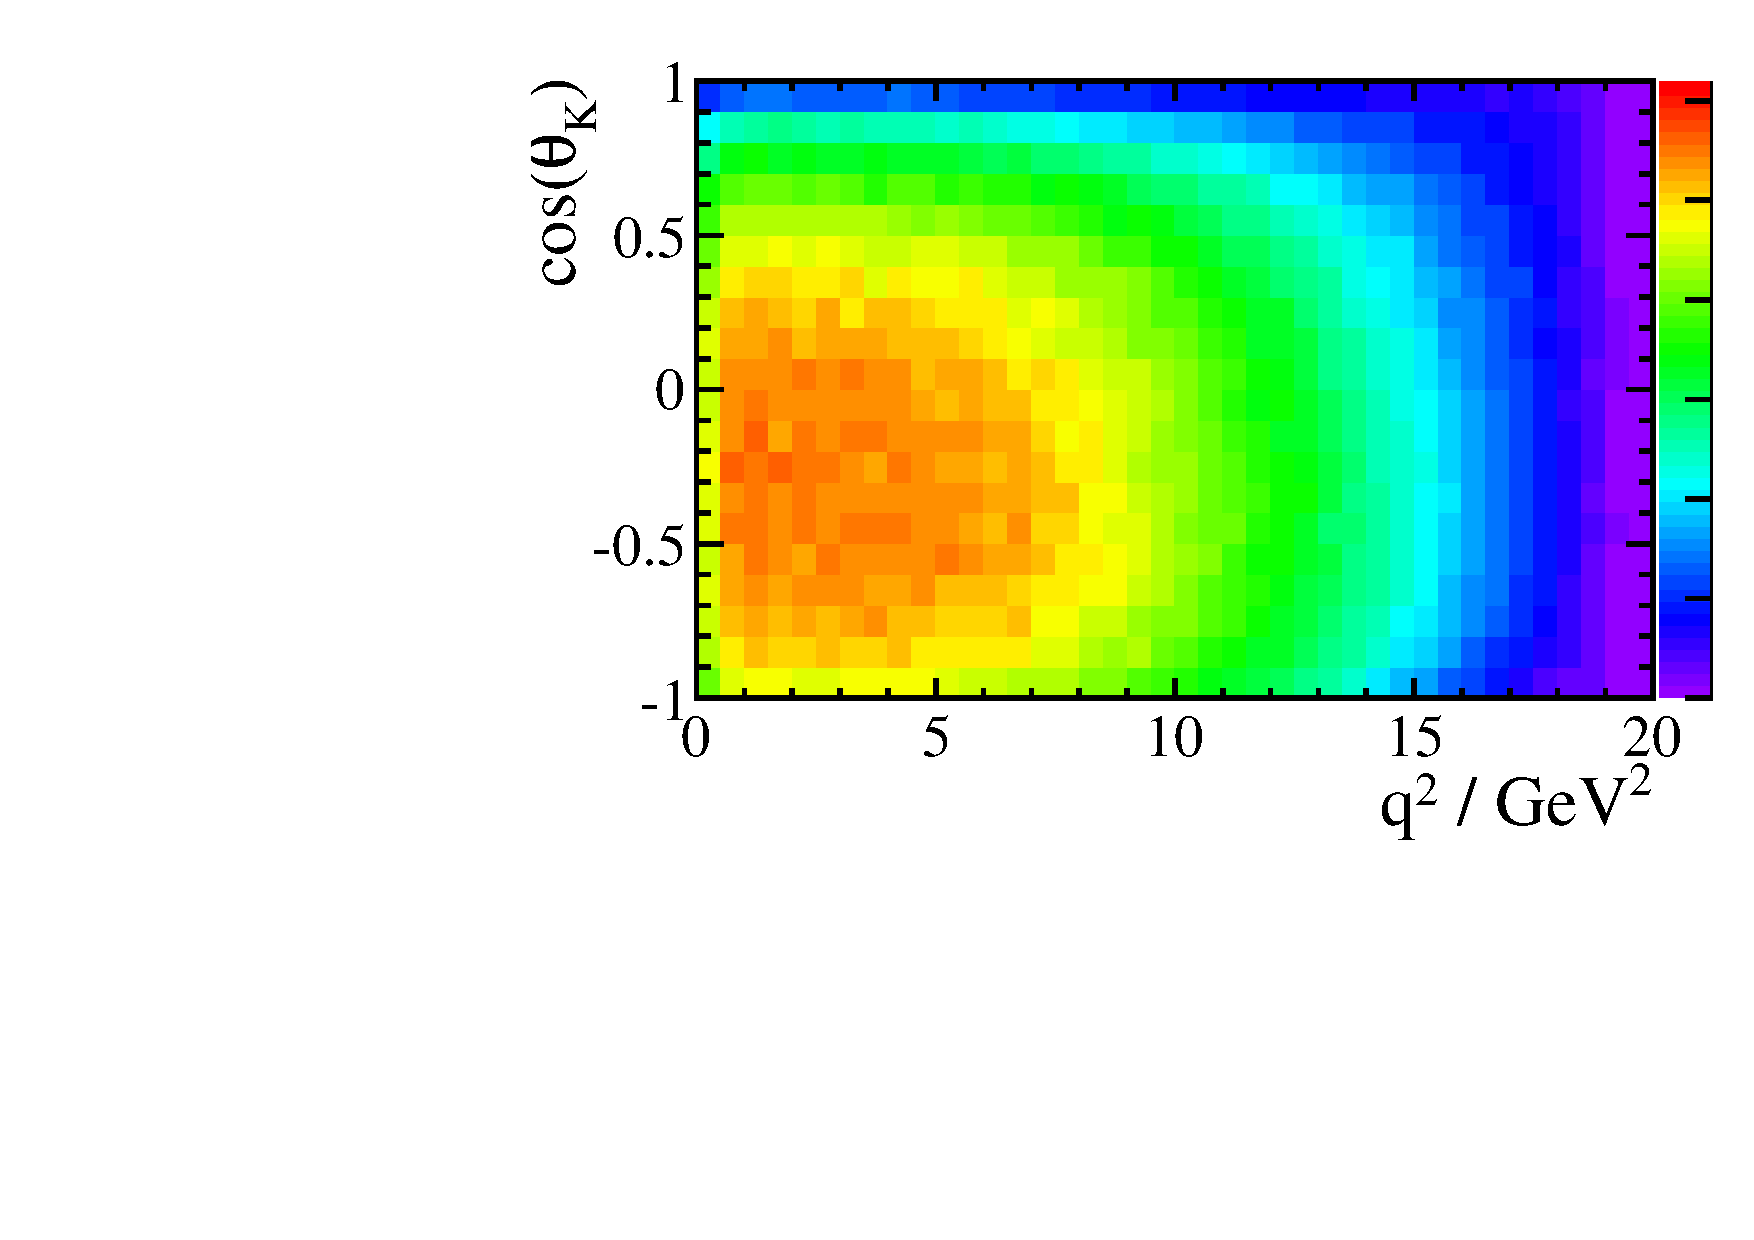
\includegraphics[width=0.48\columnwidth]{chapter5/figs/phsp_ctk_qsq_sel_dist.pdf}}
\subfigure[$\phi$ v.s. \qsq]{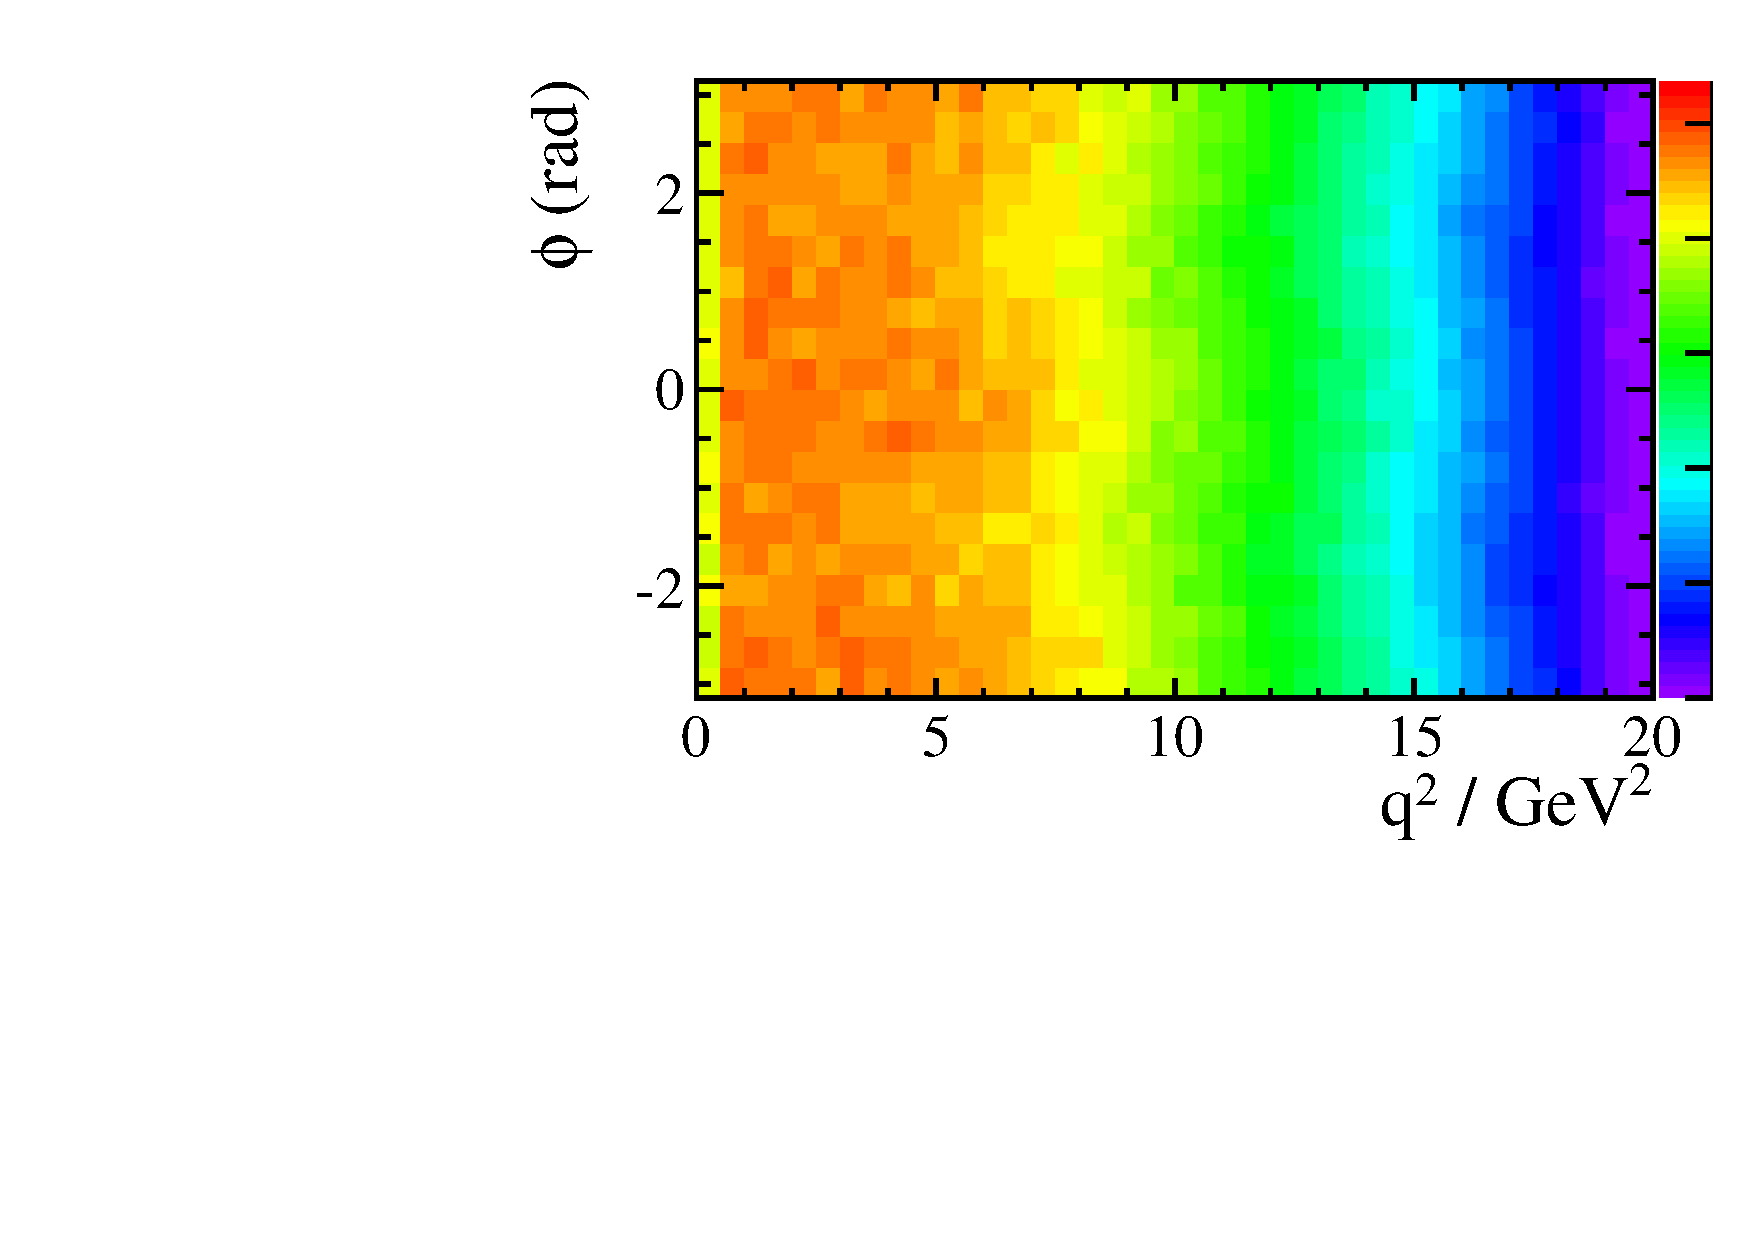
\includegraphics[width=0.48\columnwidth]{chapter5/figs/phsp_phi_qsq_sel_dist.pdf}}
\caption[Two dimensional efficiency for \BdToKstmm simulation.]
{The efficiency for selected phase space simulated \BdToKstmm events. 
In (a), (b), and (c), events are selected in the low \qsq bin ($1 < \qsq < 2 \gevgevcccc$). 
In (d), (e) and (f), the correlation between the individual angles and the full \qsq range is shown.
~\label{fig:phspeff2d} } 
\end{figure}
%It is possible to see the the efficiency is correlated with \qsq but 
%there is no significant correlation between the angles on the level of the binning shown here. 
From this it is possible to see that the efficiency function varies as \qsq, but there is no significant non-factorisable effect in the angles.
This means that the PDFs must be binned in \qsq but can be factorised between the angles.
The efficiency function for a bin in \qsq is given by 
\begin{align}
\epsilon(\ctl, \ctk, \phi, x<\qsq<y)  = \left( \frac{n_{(x<\qsq<y)} }{m_{(x<\qsq<y)} }\right) \times  S_L(\ctl) \times S_K( \ctk ) \times  S_P( \phi ) 
\end{align}
where $S_i$ is the \PDF describing the distribution of offline selected phase 
space events for each angle. 
The generator level \PDF ($G$) is uniform as a function of each of the angles and can be integrated out.

A non-uniform binning scheme was chosen to take advantage of the uneven distribution of the simulated statistics in \qsq. 
At low \qsq, where statistics are higher, bins of 0.1 \gevgevcccc are used. 
Bins of 0.2 \gevgevcccc are used in the \qsq range from 1 to 6 \gevgevcccc, and bins of 0.5 \gevgevcccc above 6 \gevgevcccc 
to the upper limit of 19\gevgevcccc .
These bins are chosen such that there are at least fifteen thousand offline 
selected events in the least populated bin from a total of two million simulated events.

The one-dimensional efficiency is modelled as a 6th order Chebychev polynomial~\cite{CHEBYCHEV}
and normalised such that the polynomial integrates to 1,
\begin{align}
\int S_i(\text{x};p_0,p_1,p_2,p_3,p_4,p_5)\ \deriv\text{x} = 1 \, ,
\end{align}
where $p_i$ are the coefficients of the polynomial. 
In order to acquire higher statistics in each \qsq bin, further reducing the error on the \PDF, 
the efficiency functions for \ctl and $\phi$ are assumed to be symmetric around 0. 
This symmetry holds to the level of CP-violating detector effects which are assumed to be less than 5\%.
The total efficiency is given by
\begin{align}
\epsilon(\qsq,\ctl,\ctk,\phi)_{(x<\qsq<y)} &= \left( \frac{n_{(x<\qsq<y)} }{m_{(x<\qsq<y)} }\right) \nonumber\\
& \times S_L(\ctl;0,a_1,0,a_3,0,a_5) \nonumber\\
& \times  S_K(\ctk;b_0,b_1,b_2,b_3,b_4,b_5) \nonumber\\
& \times S_P(\phi;0,c_1,0,c_3,0,c_5)
\end{align}
where the even (odd) parameters describe the symmetric (anti-symmetric) components of the polynomial.
The efficiency \PDFs for \ctl, \ctk and \varphi for an example low \qsq bin are shown in Fig.~\ref{fig:facpdfs}.
\begin{figure}[tbp]
\centering
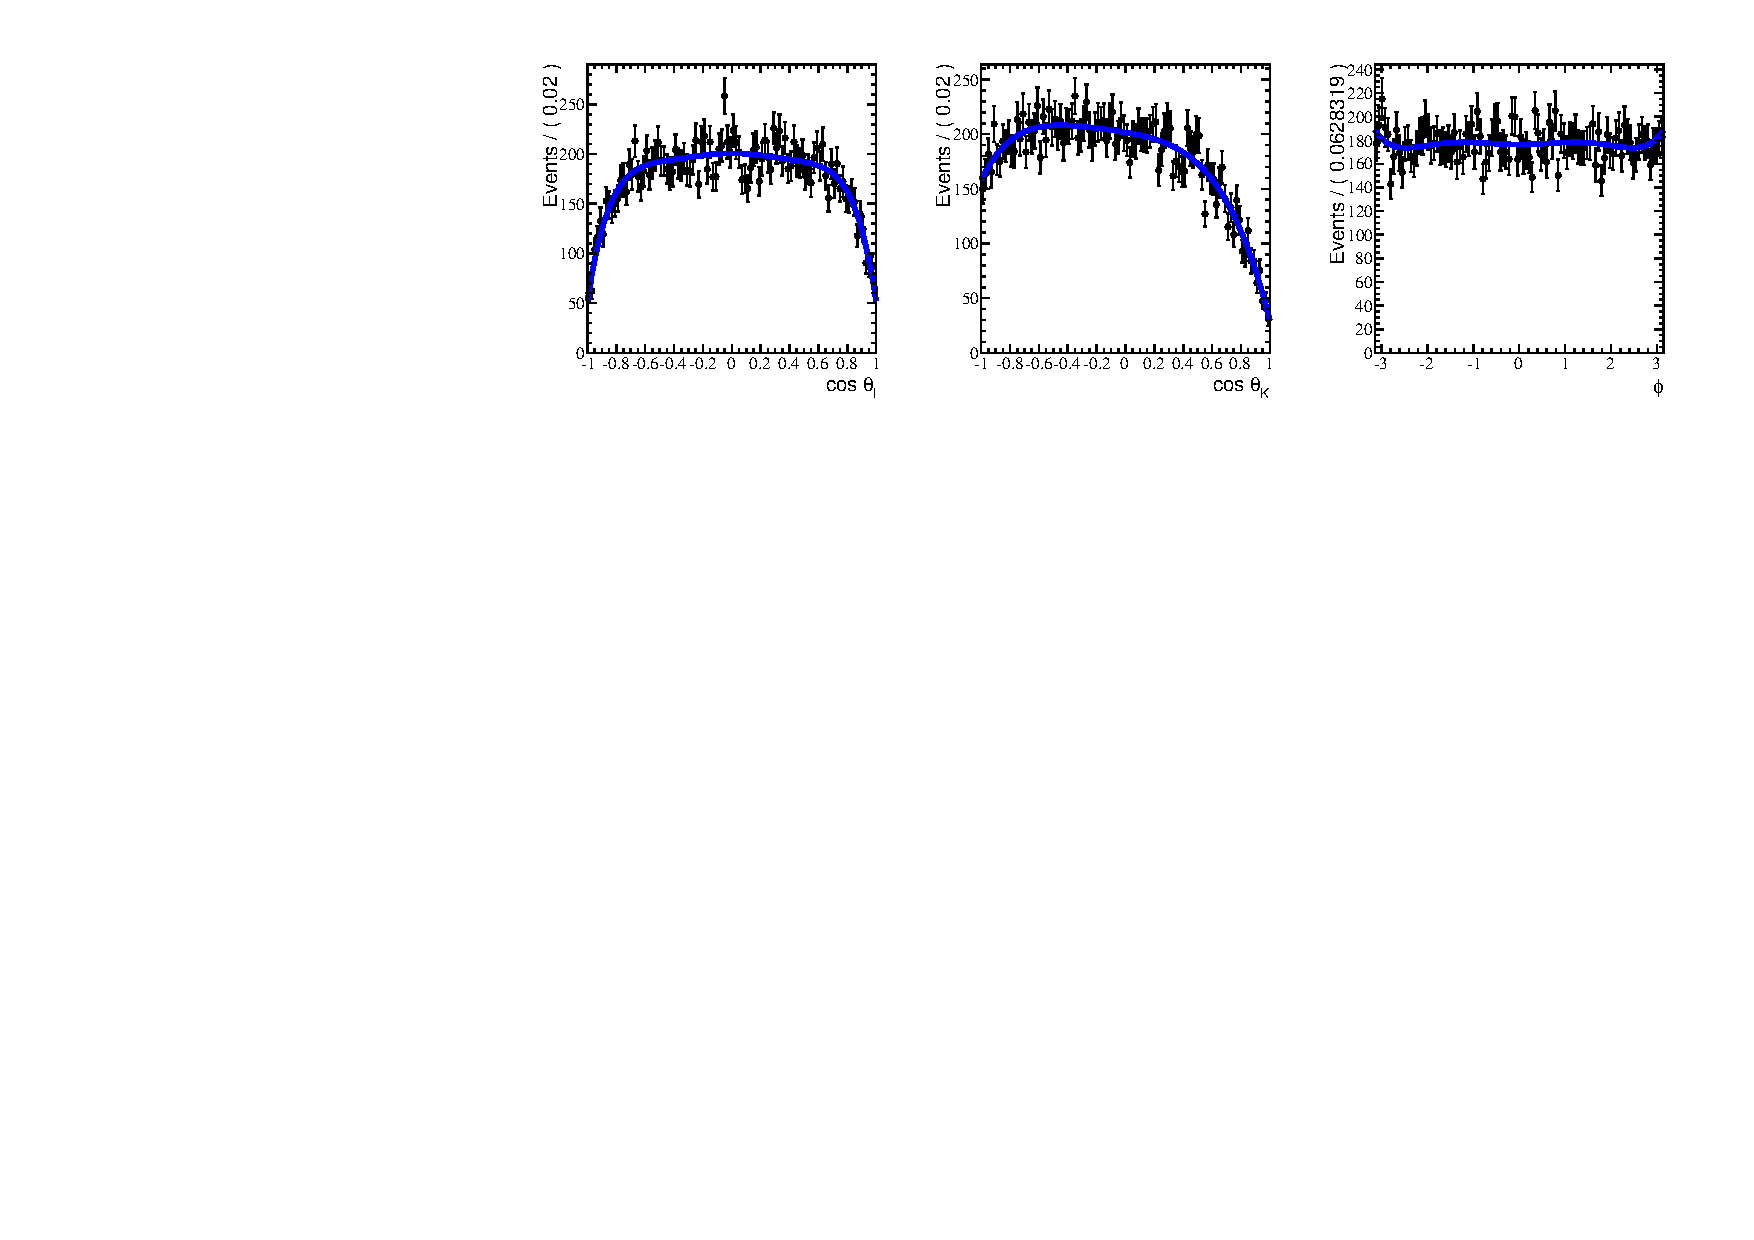
\includegraphics[width=0.96\columnwidth]{chapter5/figs/kstmm_fac_eff_pdfs_nqsqbins.pdf}
\caption[ The simulated \BdToKstmm events and the fitted PDF describing the selected events in \ctl (left), \ctk (middle)
and $\phi$ (right) for the \qsq bin from 0.1 to 0.2 \gevgevcccc.]
{ The angular efficiency in each of the angles for the \qsq bin from 0.1 to 0.2 \gevgevcccc.
The factorised \PDF was fitted to phase space \BdToKstmm simulation. ~\label{fig:facpdfs} }
\end{figure}

The distribution of weights on ten thousand phase space events is given in Fig~\ref{fig:ac2weights}.
\begin{figure}[tbp]
\centering
\subfigure[]{\includegraphics[width=0.48\columnwidth]{chapter5/figs/ac2/phasespace_weight_value.pdf}}
\subfigure[]{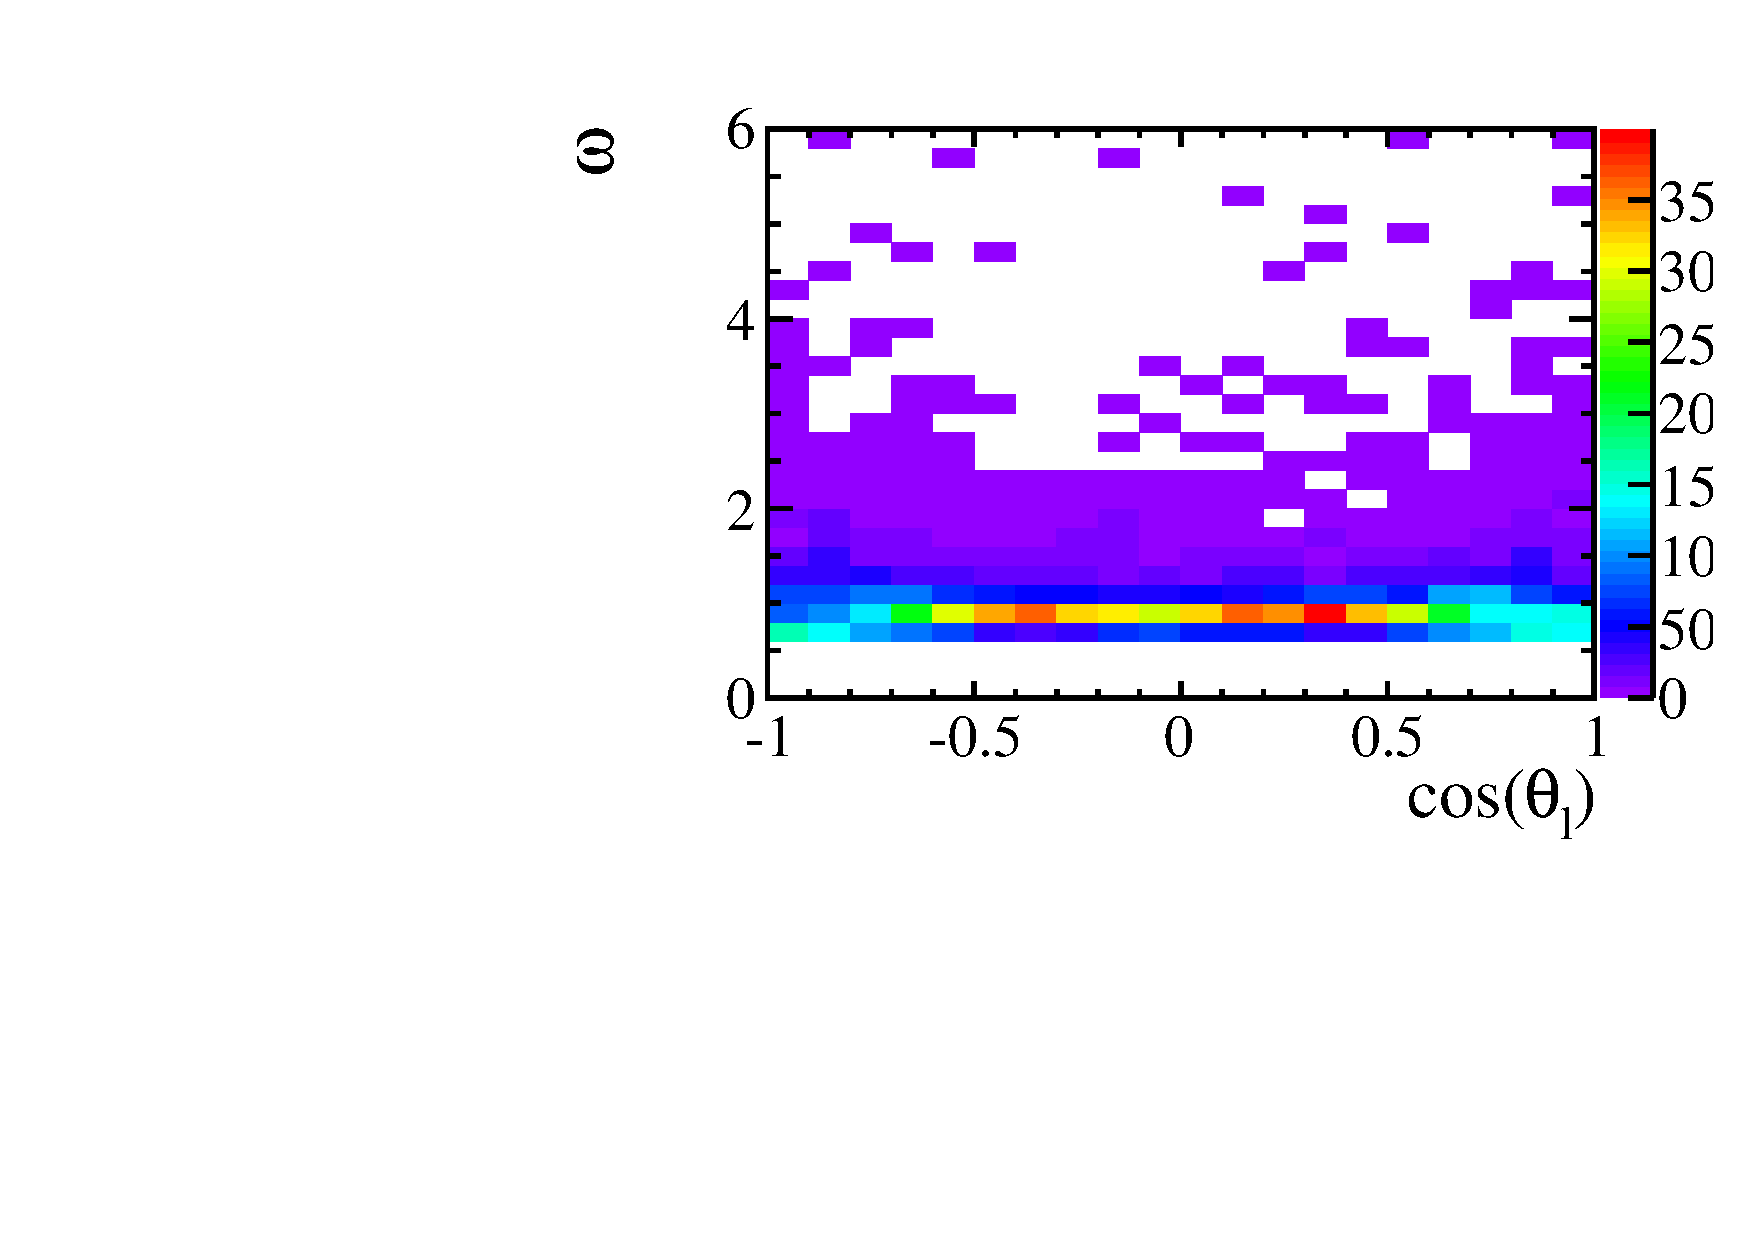
\includegraphics[width=0.48\columnwidth]{chapter5/figs/ac2/phasespace_weight_ctl.pdf}}
\subfigure[]{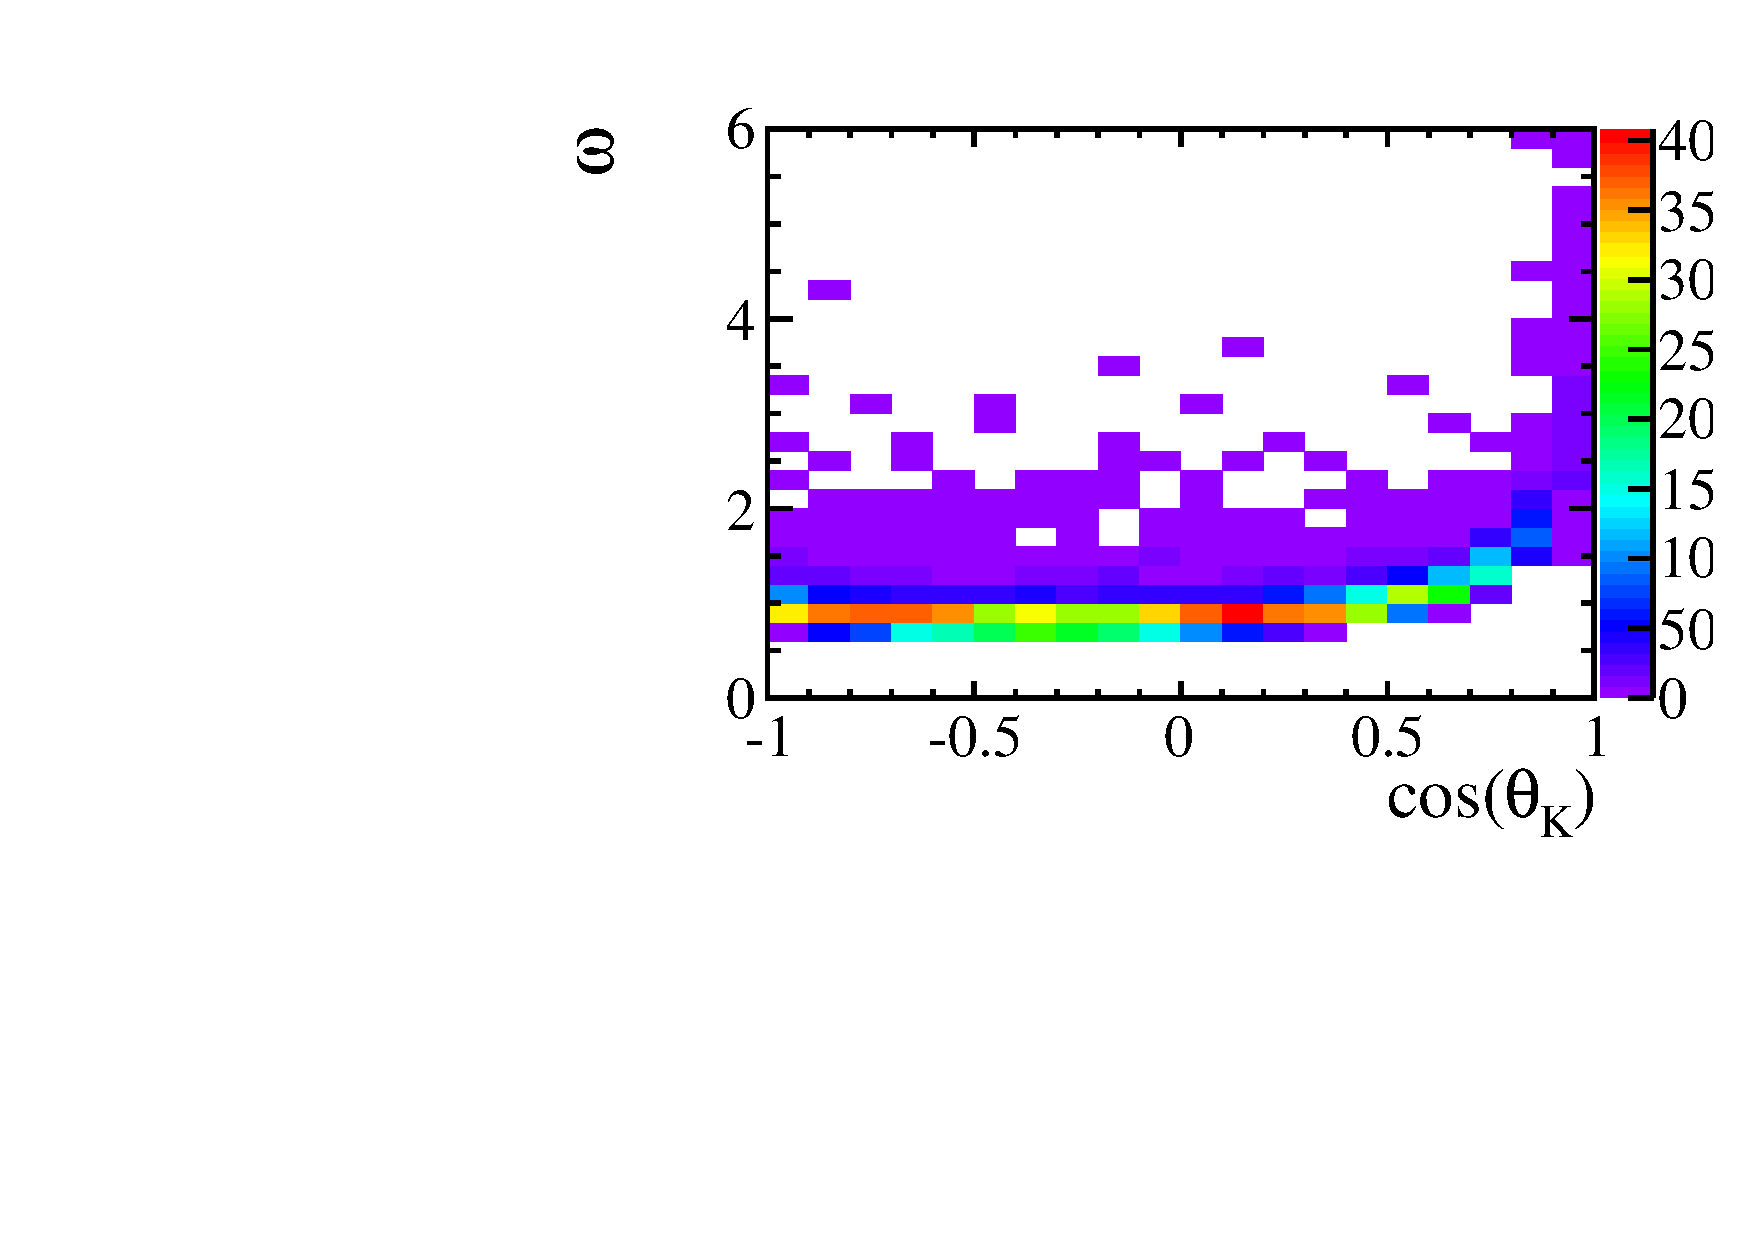
\includegraphics[width=0.48\columnwidth]{chapter5/figs/ac2/phasespace_weight_ctk.pdf}}
%\subfigure[]{\includegraphics[width=0.48\columnwidth]{chapter5/figs/ac2/phasespace_weight_phi.pdf}}
\caption[ The distribution of weights for 10000 phase space simulated \BdToKstmm events.] 
{ The distribution of weights for 10000 phase space simulated \BdToKstmm events and the correlation between 
the weights and \ctl and \ctk. The weights are normalised such that the sum of weights is equal to the 
number of events. The high weights for extreme \ctk and \ctl can be seen. ~\label{fig:ac2weights} }
\end{figure}
The larger weights for extreme \ctl and \ctk regions can be seen.% along with a small variation in \varphi.

\subsubsection{Testing the factorisation}
\label{sec:kstmm:facac:nonfac}

The assumption that the efficiency can be factorised is tested and 
the quality of the fit are assessed by using a variation of the binned $\chi^2$ test.
This modified test compares the distribution of data events used to fit a \PDF to the 
distribution of toy Monte Carlo events generated from the fitted \PDF.
The number of toy Monte Carlo events generated from the fitted \PDF 
using an accept/reject method was scaled to one hundred times the number of data events.
The phase space of \ctl, \ctk and $\phi$ was divided up into one thousand bins.
The pull value for each bin is calculated from
\begin{align}
p^i = n^{i}_{Data} - \left(\frac{n_{Data}^i - 10^{-2} n^{i}_{MC} }{ \sigma }\right)
\end{align}
where the error is defined as
\begin{align}
\sigma = \sqrt{( n_{Data}^i + 10^{-2} n_{MC} )} \, .
\end{align}
If the \PDF is a good fit to the data then the pull values should be normally distributed.
Here the `data' is the offline selected sample of phase space \BdToKstmm simulated events. 
Pull distributions for one low and one high \qsq bin are shown in Fig.~\ref{fig:facpulldist}.
\begin{figure}[tbp]
\centering
\subfigure[]{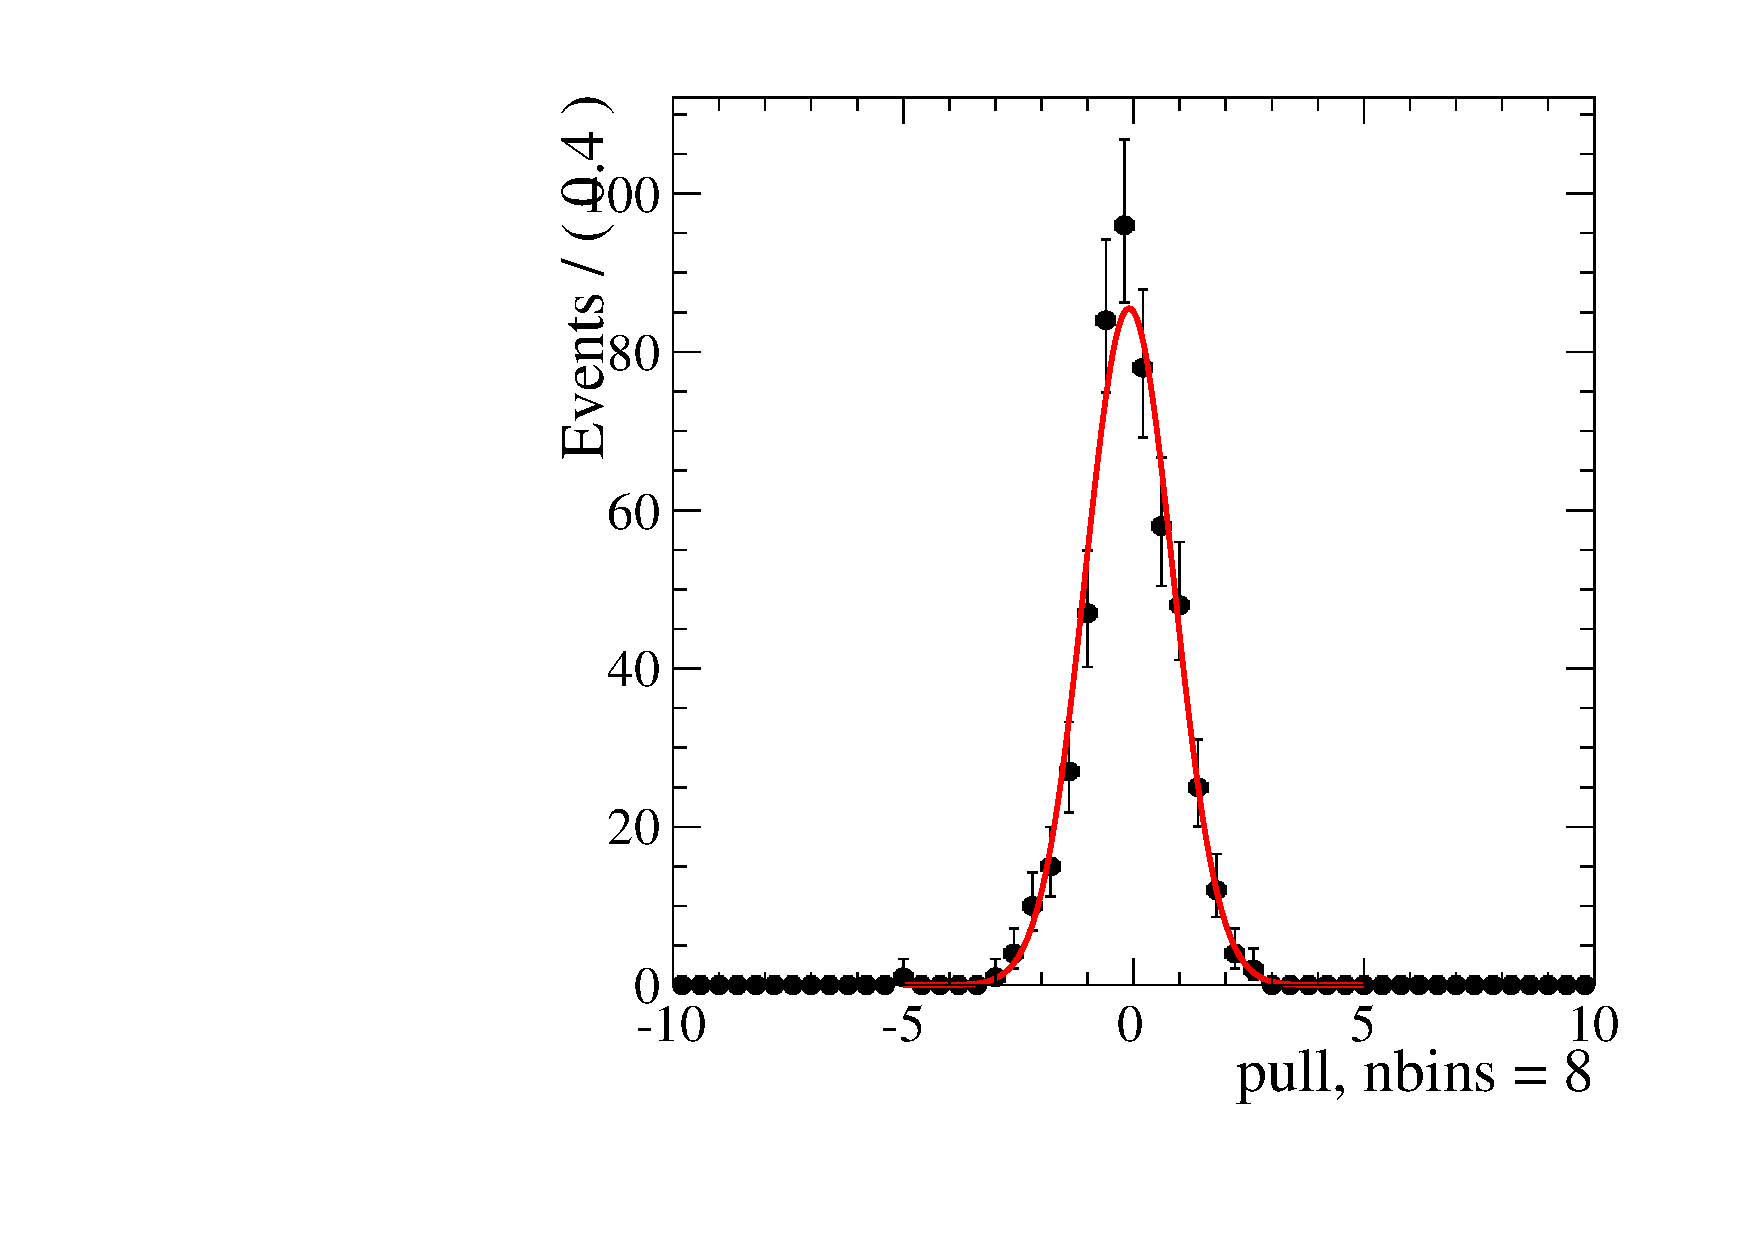
\includegraphics[width=0.48\columnwidth,page=1]{chapter5/figs/pull_dist_qsq_bins.pdf}}
\subfigure[]{\includegraphics[width=0.48\columnwidth,page=50]{chapter5/figs/pull_dist_qsq_bins.pdf}}
\caption [ The pull distribution of a toy simulation from the factorised \PDFs.] 
{ The pull distribution of a toy simulation from the factorised \PDFs.
A low \qsq bin (a) ($1<\qsq<2\gevgevcccc$) and a high \qsq bin (b) ($15<\qsq<15.5\gevgevcccc$). 
The fit for both distributions is compatible with a Gaussian of zero mean and unit width. ~\label{fig:facpulldist} }
\end{figure}
Both pull distributions are compatible with a Gaussian with zero mean and unit width.
The mean and width of the pull distribution for each bin in \qsq are given in Fig.~\ref{fig:facpulldistall}.
\begin{figure}[tbp]
\centering
\subfigure[]{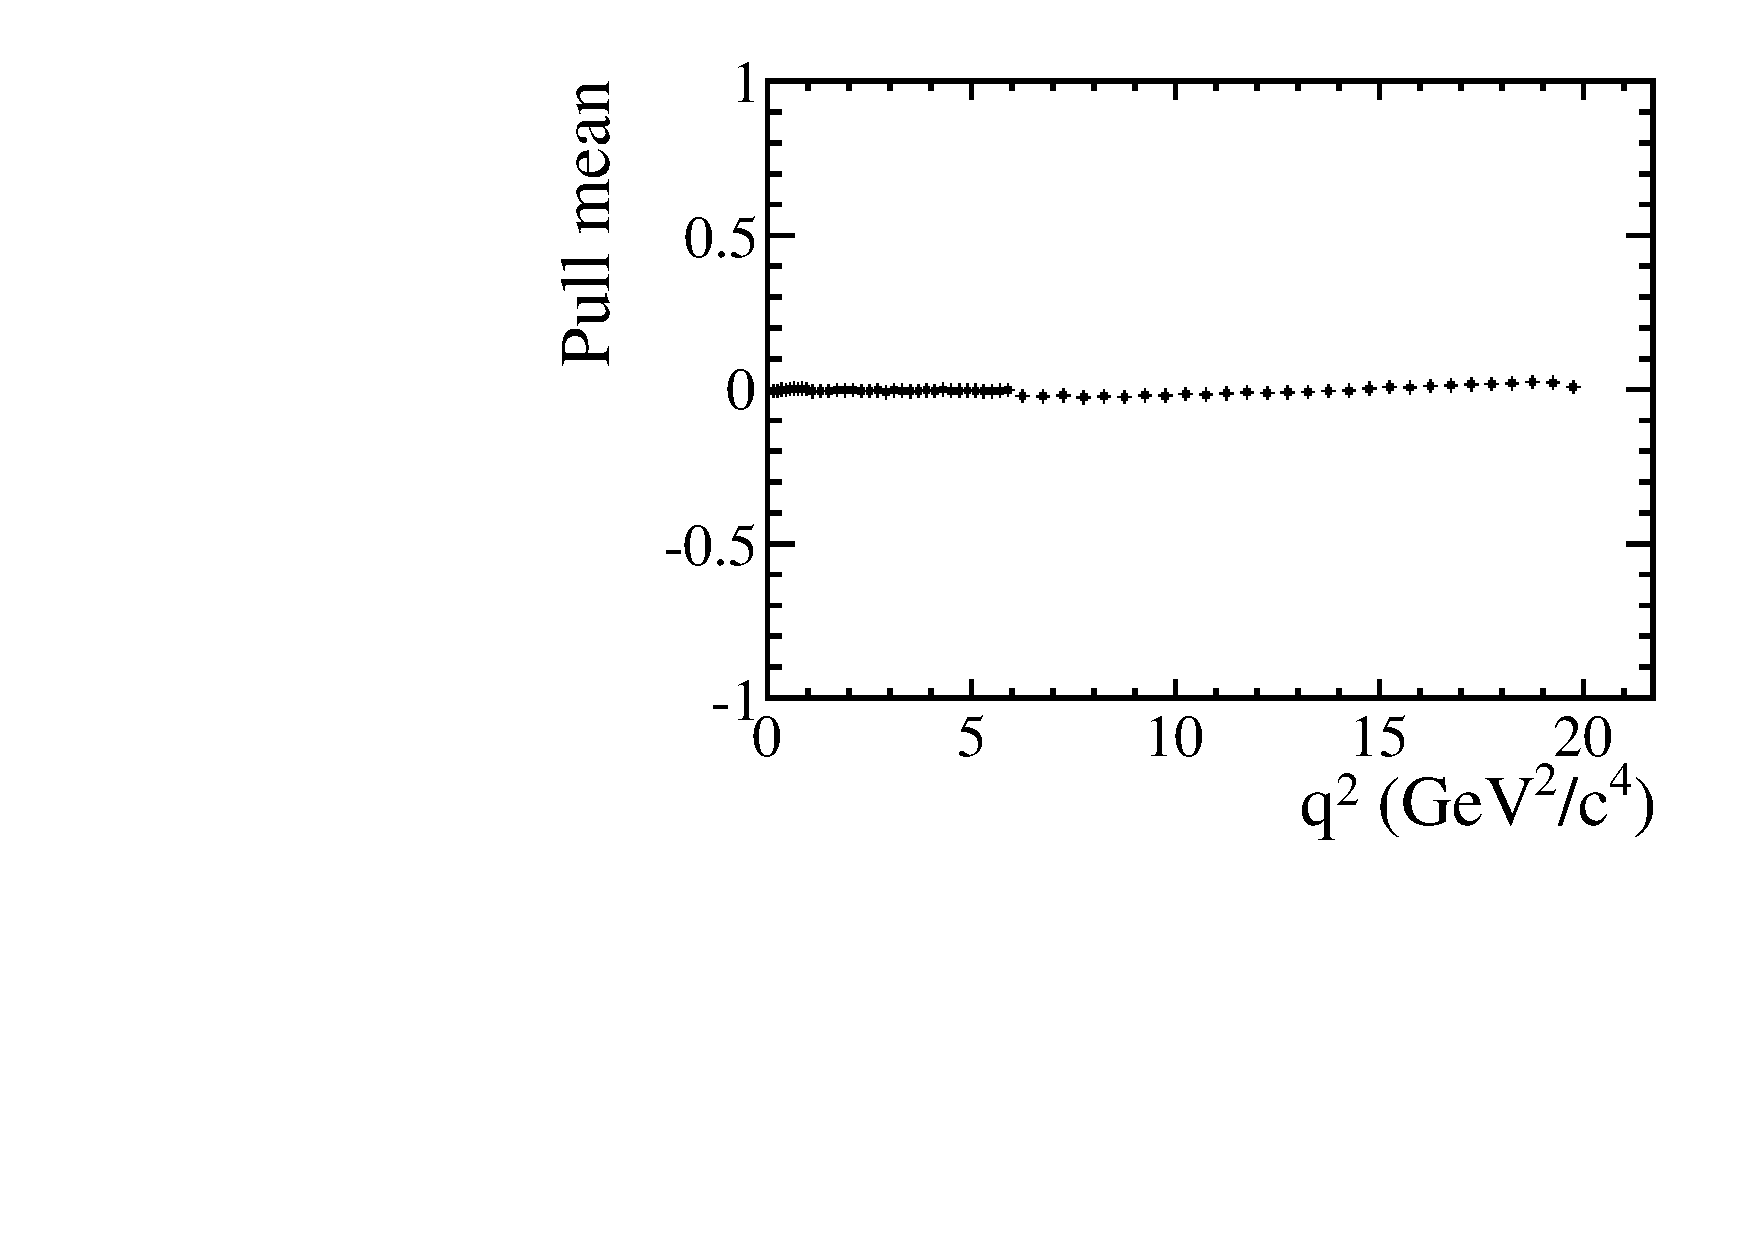
\includegraphics[width=0.48\columnwidth]{chapter5/figs/ac2/fiteff_results_62_pull_meangraph.pdf}}
\subfigure[]{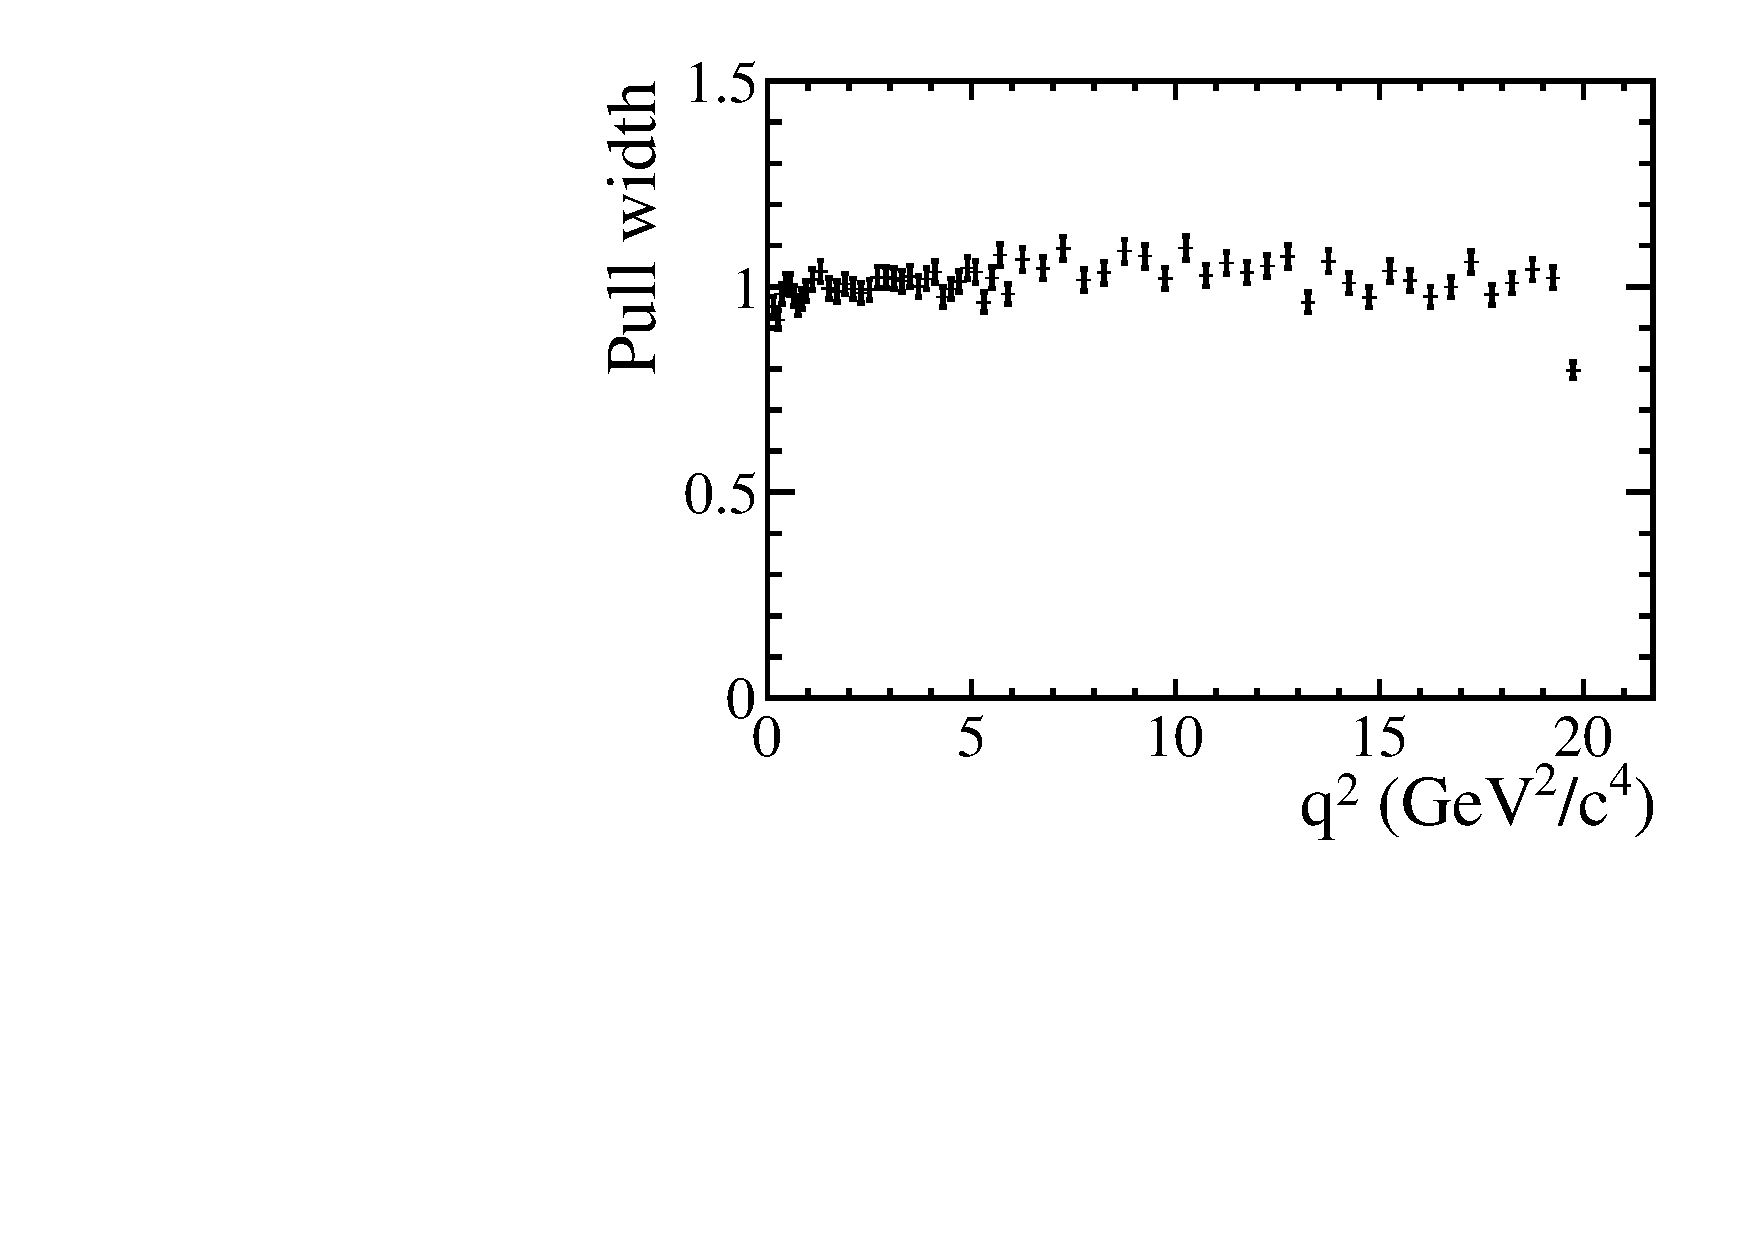
\includegraphics[width=0.48\columnwidth]{chapter5/figs/ac2/fiteff_results_62_pull_pullgraph_new.pdf}}
\caption [ The pull distribution of a toy simulation from the factorised \PDFs.] 
{ The (a) mean and (b) width of each pull distribution of a toy simulation from the factorised \PDFs in bins of \qsq.
The bins are all compatible with a Gaussian of zero mean and unit width. ~\label{fig:facpulldistall} }
\end{figure}
This shows that there are no regions of great discrepancy between the simulation and the factorised \PDF in these bins of \qsq.

The factorisation of the efficiency allows for a more precise acceptance correction at the cost of incurring a 
possible source of systematic uncertainty associated with integrating over non-factorisable effects.
The factorisation was also tested by comparing the re-weighted phase space simulated events to the 
generator level distributions in each of the factorised dimensions.

%The degree to which non-factorisable effects can be ignored is tested by
%multiplying the efficiency function with a non-factorisable function,
%\begin{align}
%f(\ctl,\ctk) = 1 + \alpha\sin(\pi\ctl)\sin(\pi\ctk)
%\end{align}
%where $\alpha$ is a scaling factor. The efficiency function is modelled as
%\begin{align}
%\epsilon^{'}(\qsq,\ctl,\ctk,\phi)_{(x<\qsq<y)} = \epsilon(\qsq,\ctl,\ctk,\phi)_{(x<\qsq<y)} \times f(\ctl,\ctk) \, .
%\end{align}
%The mean and width of a Gaussian fit to the pull distributions for various values of $\alpha$
%are shown in Fig.~\ref{fig:nonfactest}.
%\begin{figure}[tbp]
%\centering
%\dots
%\caption{ The pull mean and pull width for a Gaussian fit to the pull distribution between simulation and 
%toy Monte Carlo generated from the fitted efficiency as a function of the non-factorisable 
%scaling factor, $\alpha$. ~\label{fig:nonfactest} }
%\end{figure}

\subsection{Re-weighted phase space distributions}

The most basic test of an acceptance correction is that the original generator 
level distribution used to create the acceptance correction can be recovered.
In this case the phase space distribution %given in Fig.~\ref{fig:phsp}
should be recovered when the phase space candidates are themselves weighted.
The number of re-weighted \BdToKstmm candidates per bin in phase space is given by 
\begin{align}
N_{\text{bin}} = \sum_{i=1}^{ncand} \frac{1}{\epsilon(\ctl,\ctk,\phi)_i} = \sum_{i=1}^{ncand} \omega_i .
\end{align}
which can be compared to the expected number of generator level events in that bin. 

The weighted distributions for the $k$-nearest-neighbour acceptance correction method are shown in
Fig.~\ref{fig:corrphsp1}.
\begin{figure}[tbp]
\centering
\subfigure[]{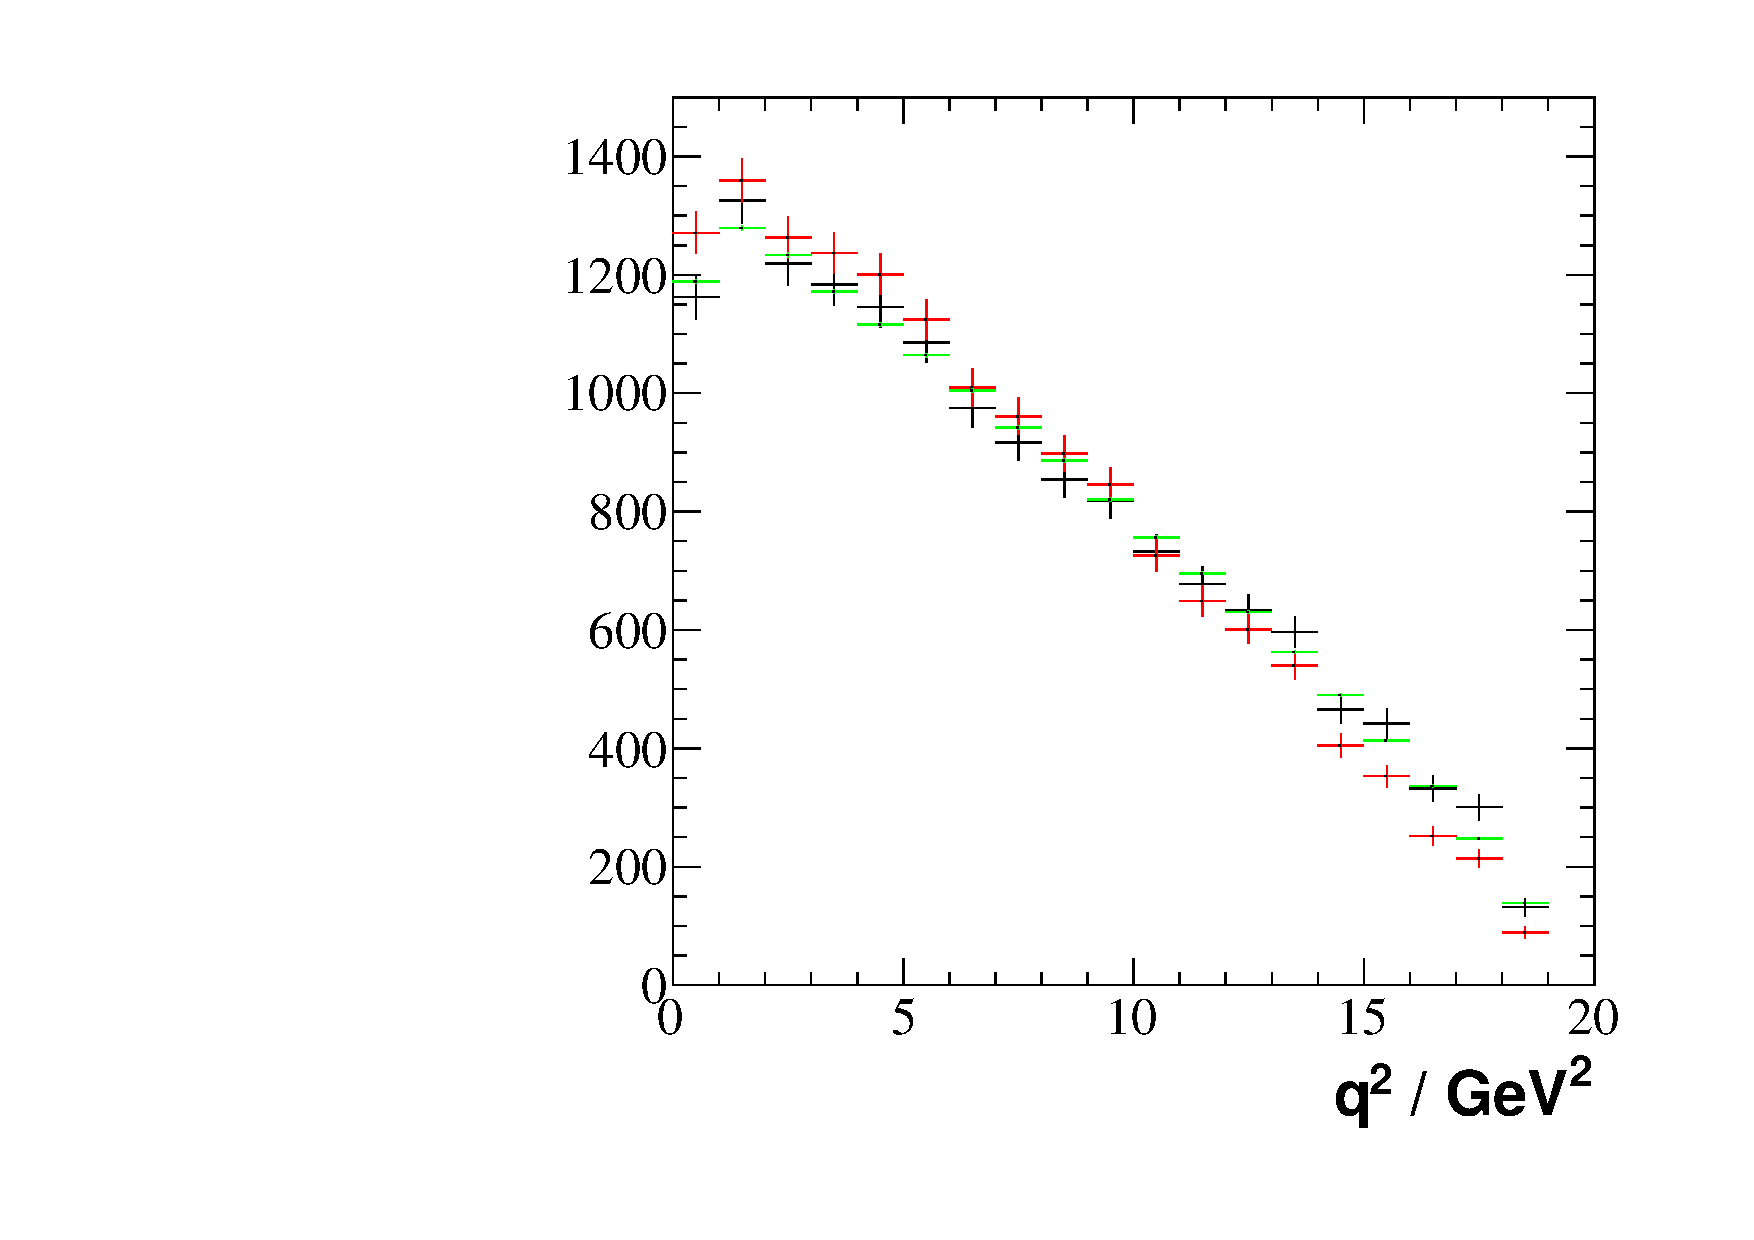
\includegraphics[width=0.32\columnwidth]{chapter5/figs/ac1/CorrectionsWithGen_Qsquare.pdf}}
\subfigure[]{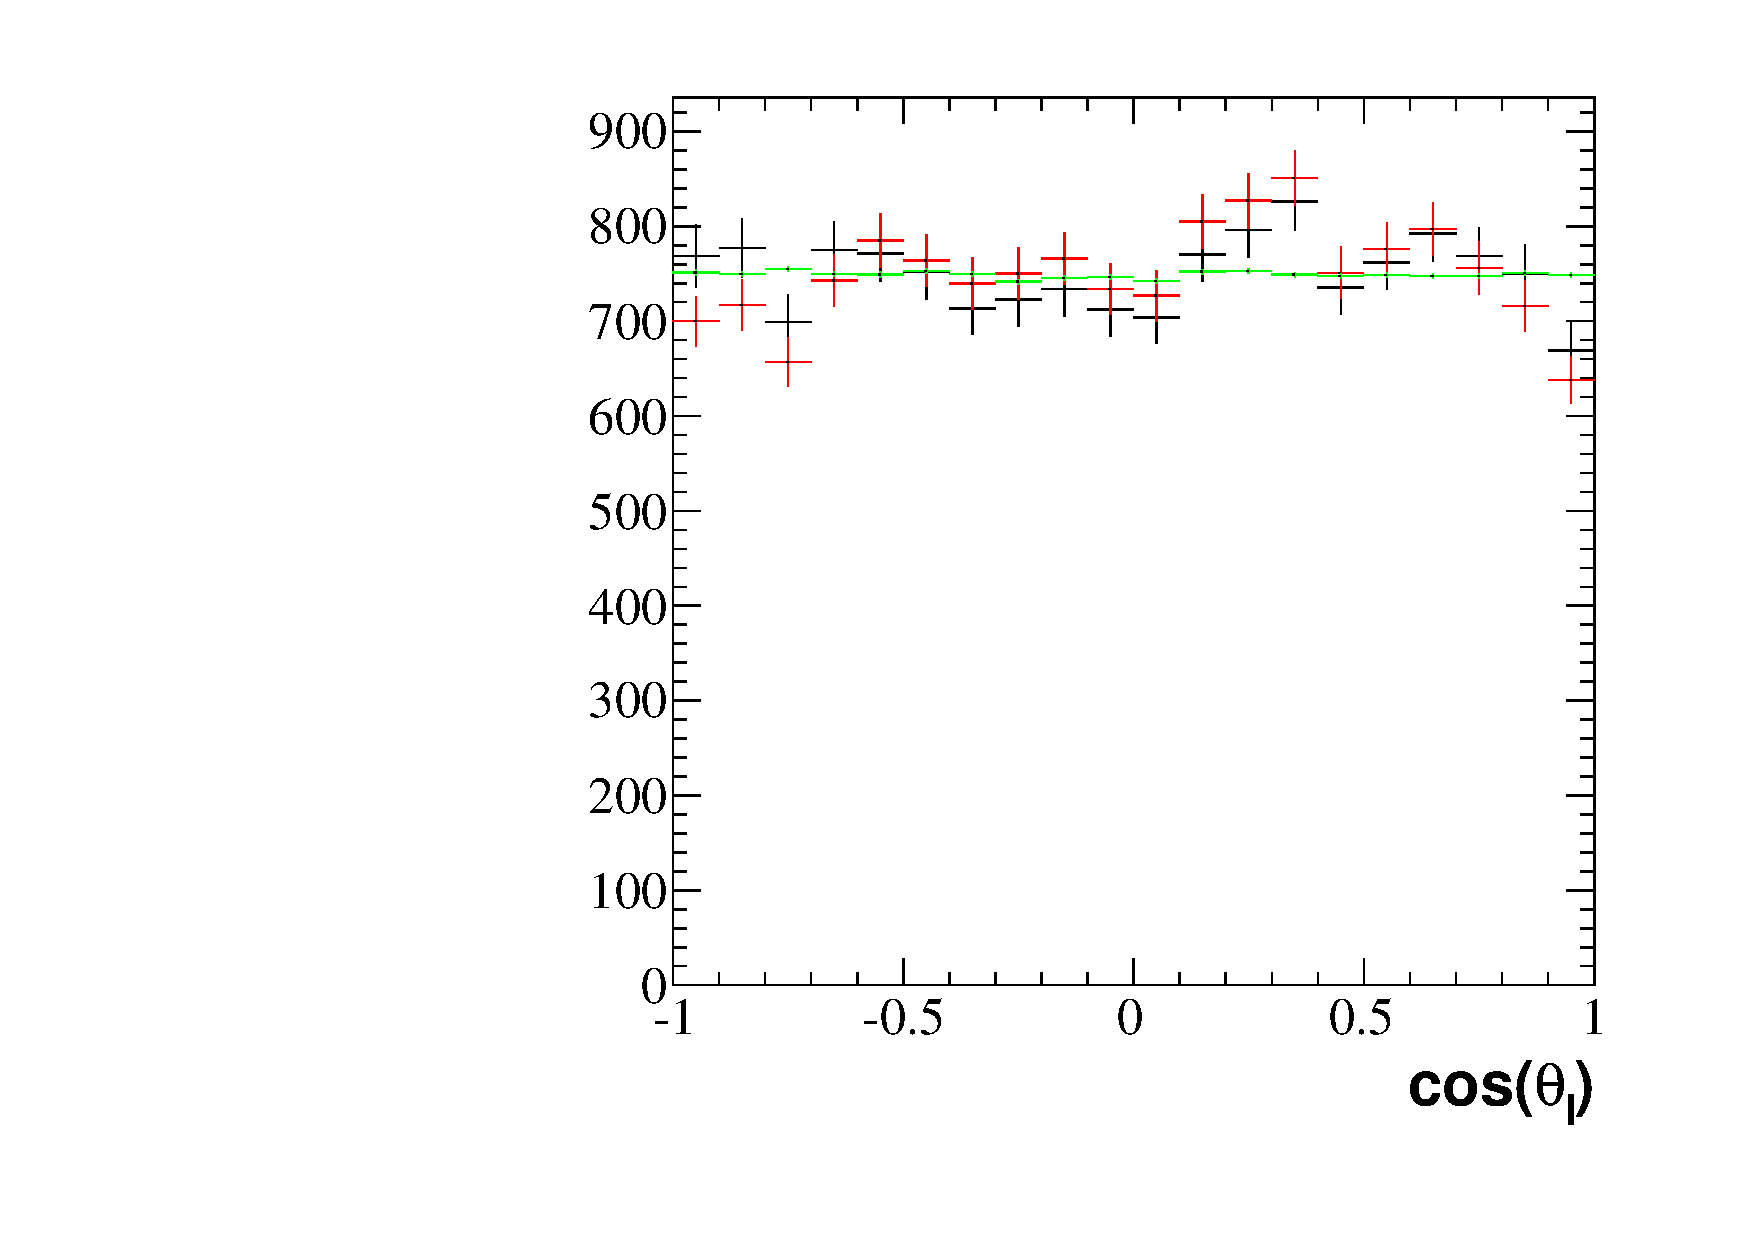
\includegraphics[width=0.32\columnwidth]{chapter5/figs/ac1/CorrectionsWithGen_ThetaL.pdf}}
\subfigure[]{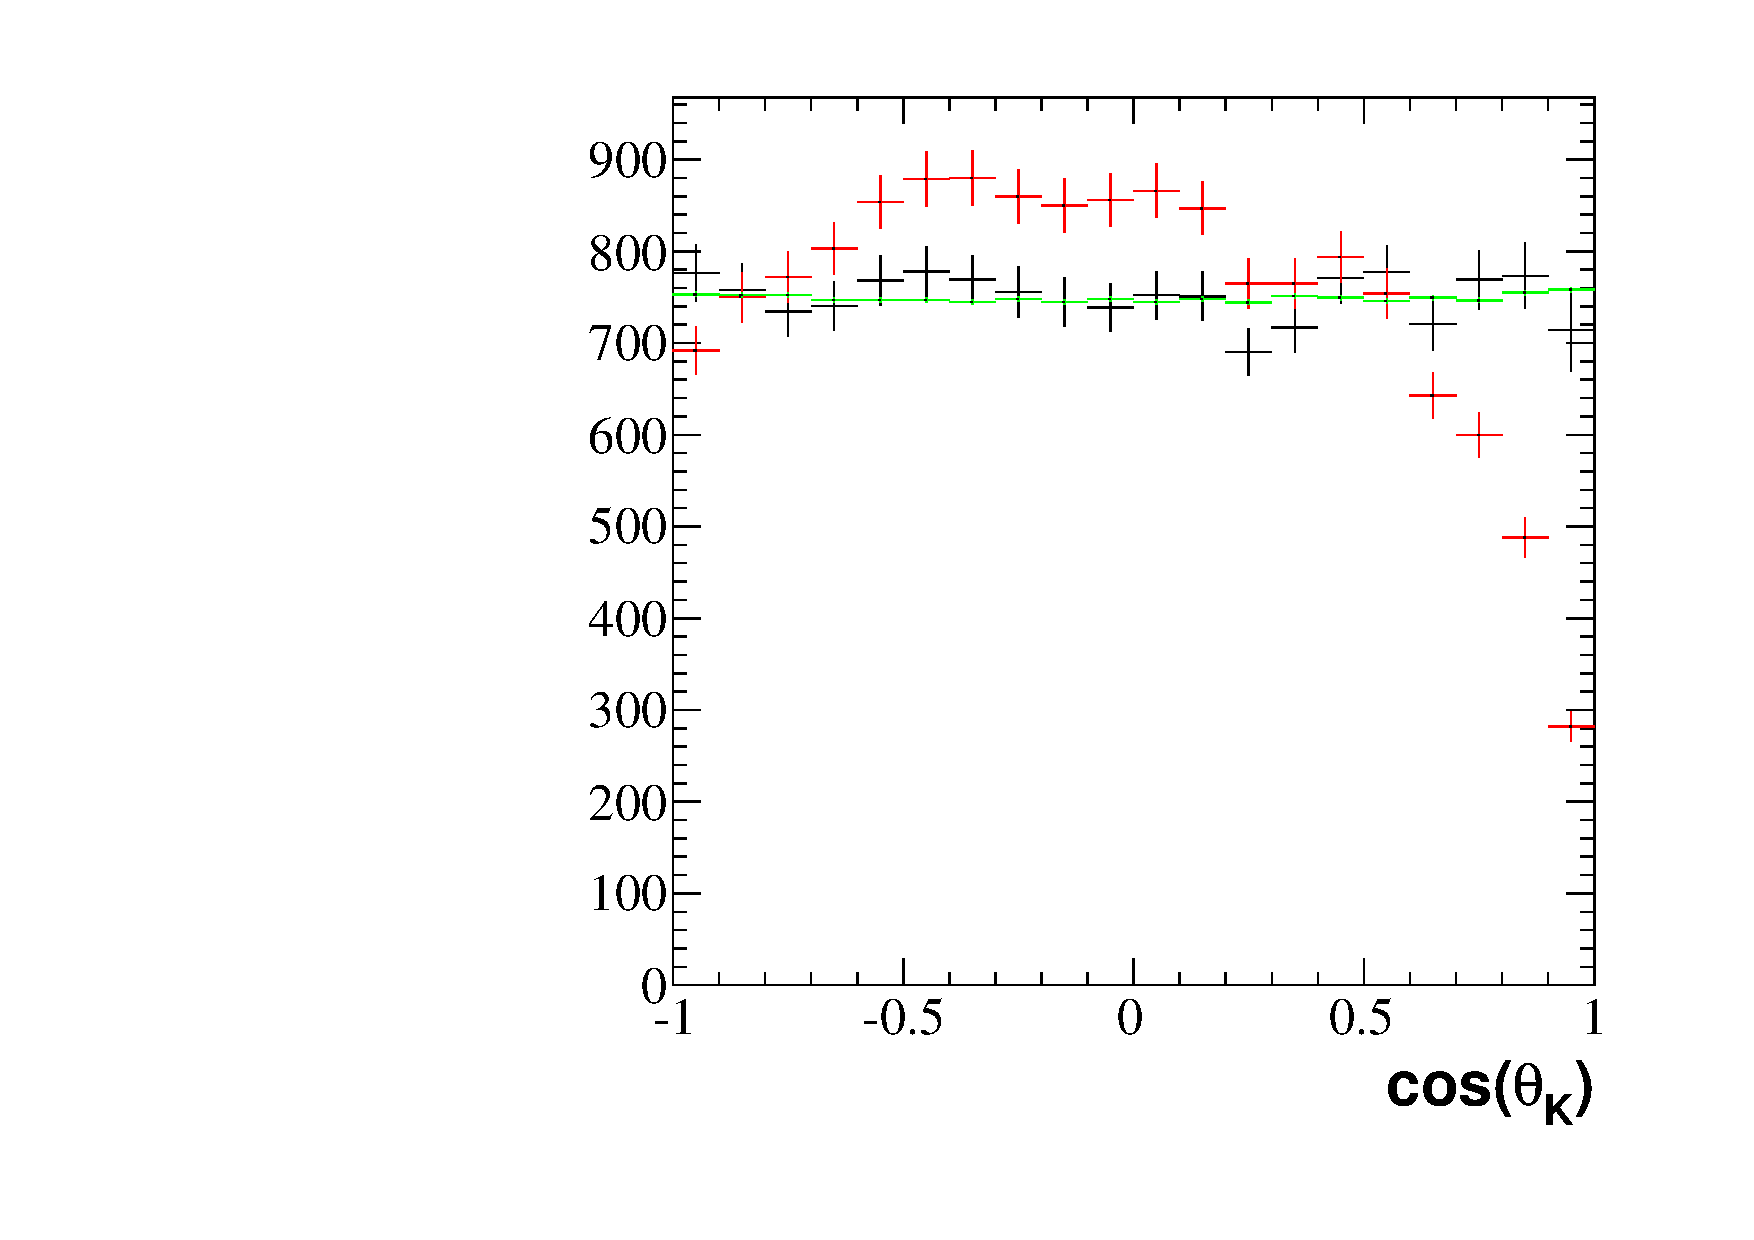
\includegraphics[width=0.32\columnwidth]{chapter5/figs/ac1/CorrectionsWithGen_ThetaK.pdf}}
\caption{Generated (green), offline selected (red) and re-weighted (black) events for  \BdToKstmm using the 
$k$-nearest-neighbour acceptance correction method.~\label{fig:corrphsp1}}
\end{figure}
Is it possible to see that the efficiency at extreme \ctk and extreme \ctl is recovered. 

The weighted distributions for the factorised acceptance correction method are shown in Fig.~\ref{fig:corrphsp2}.
\begin{figure}[tbp]
\centering
\subfigure[]{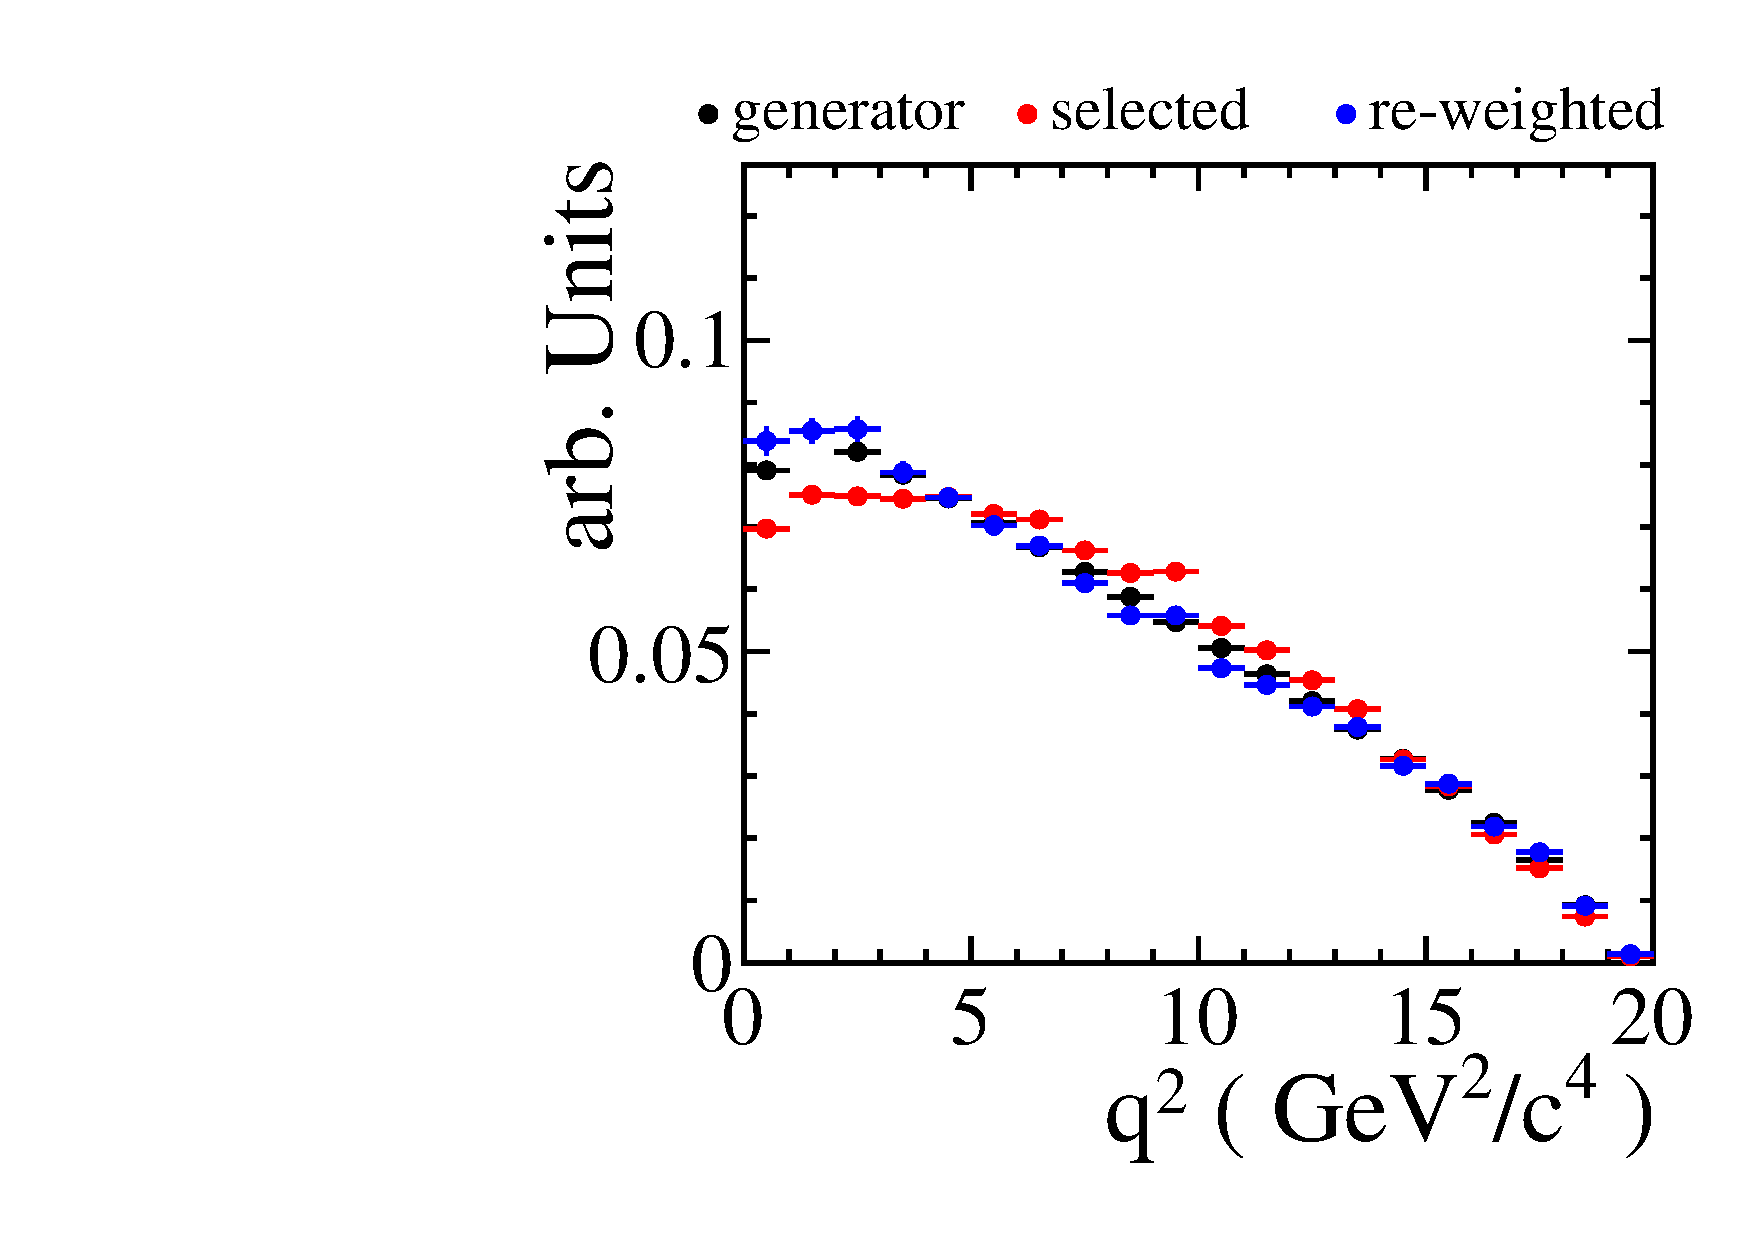
\includegraphics[width=0.48\columnwidth]{chapter5/figs/ac2/CorrectionsWithGen_Qsquare_new.pdf}}
\subfigure[]{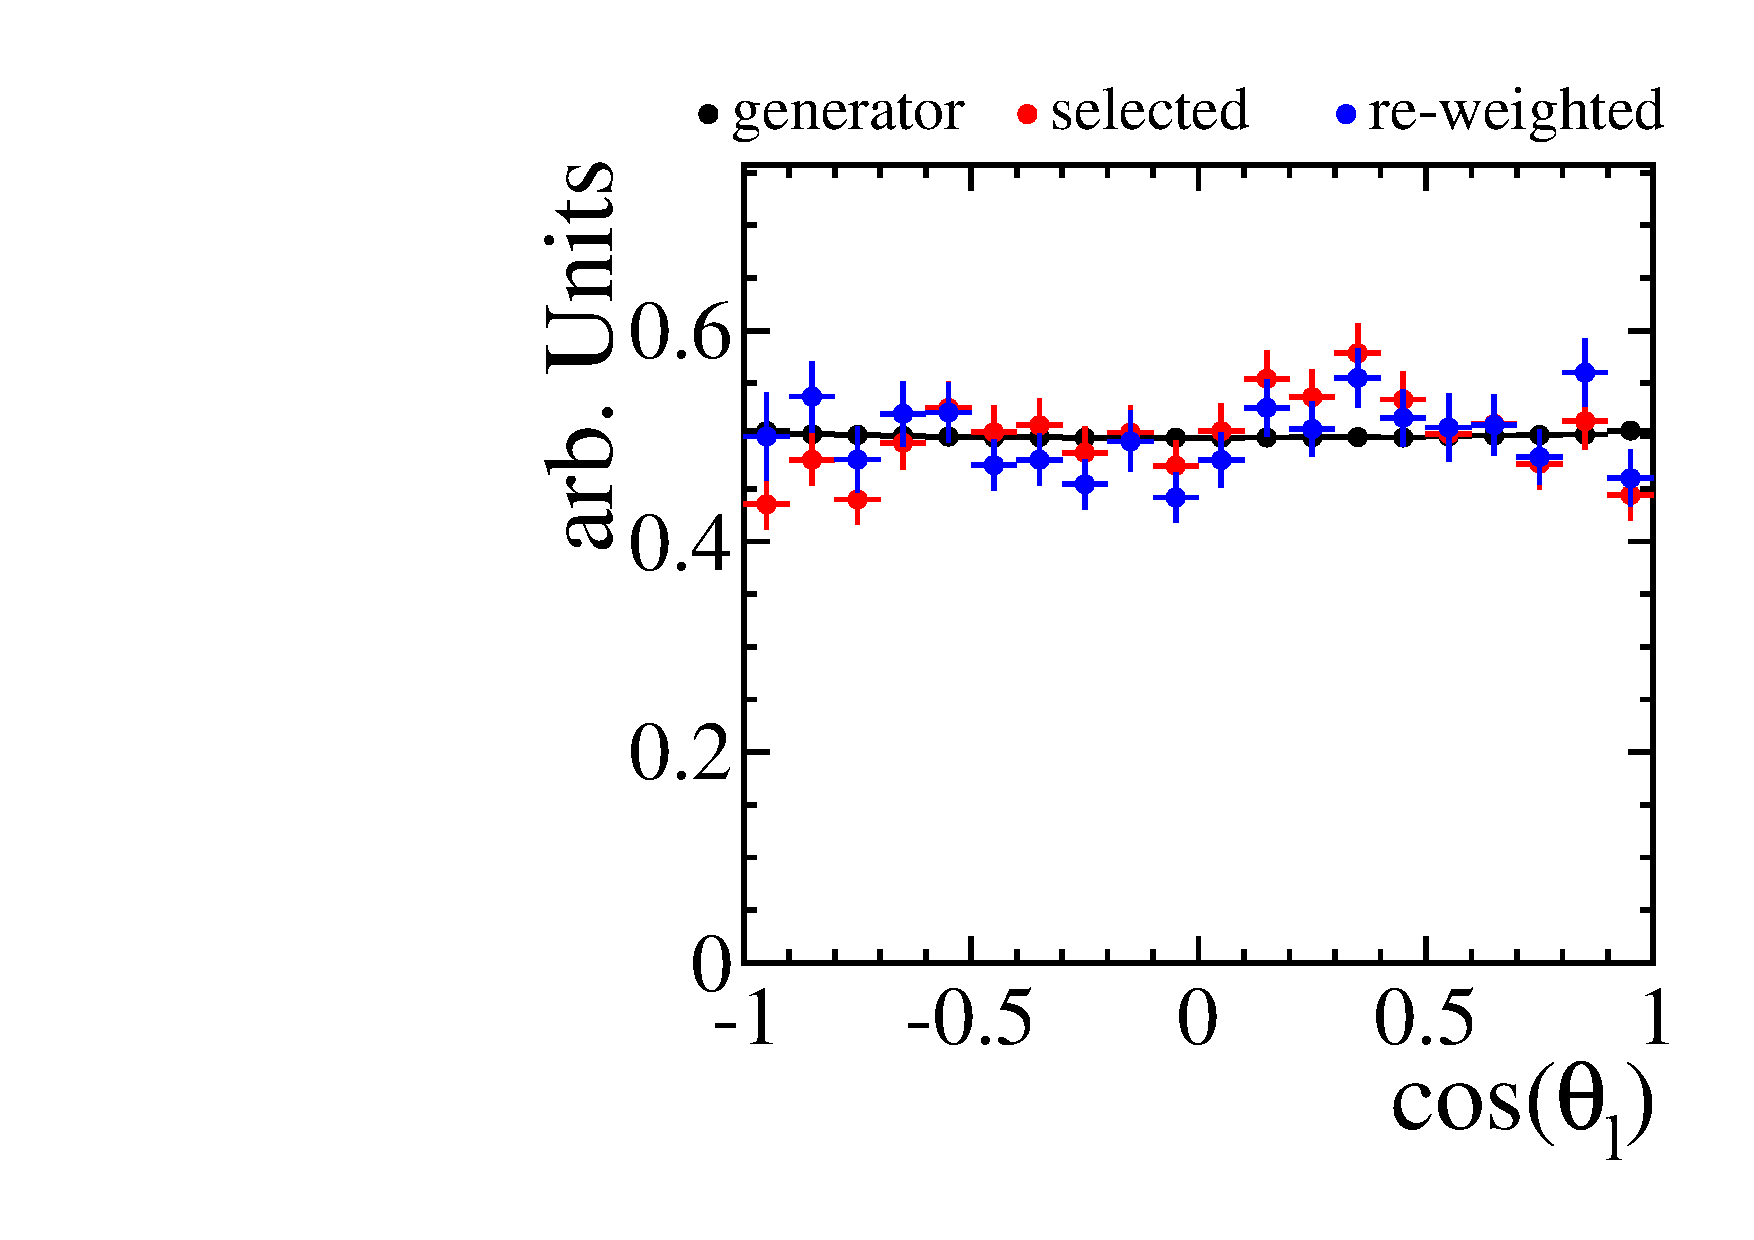
\includegraphics[width=0.48\columnwidth]{chapter5/figs/ac2/CorrectionsWithGen_ThetaL_new.pdf}}
\subfigure[]{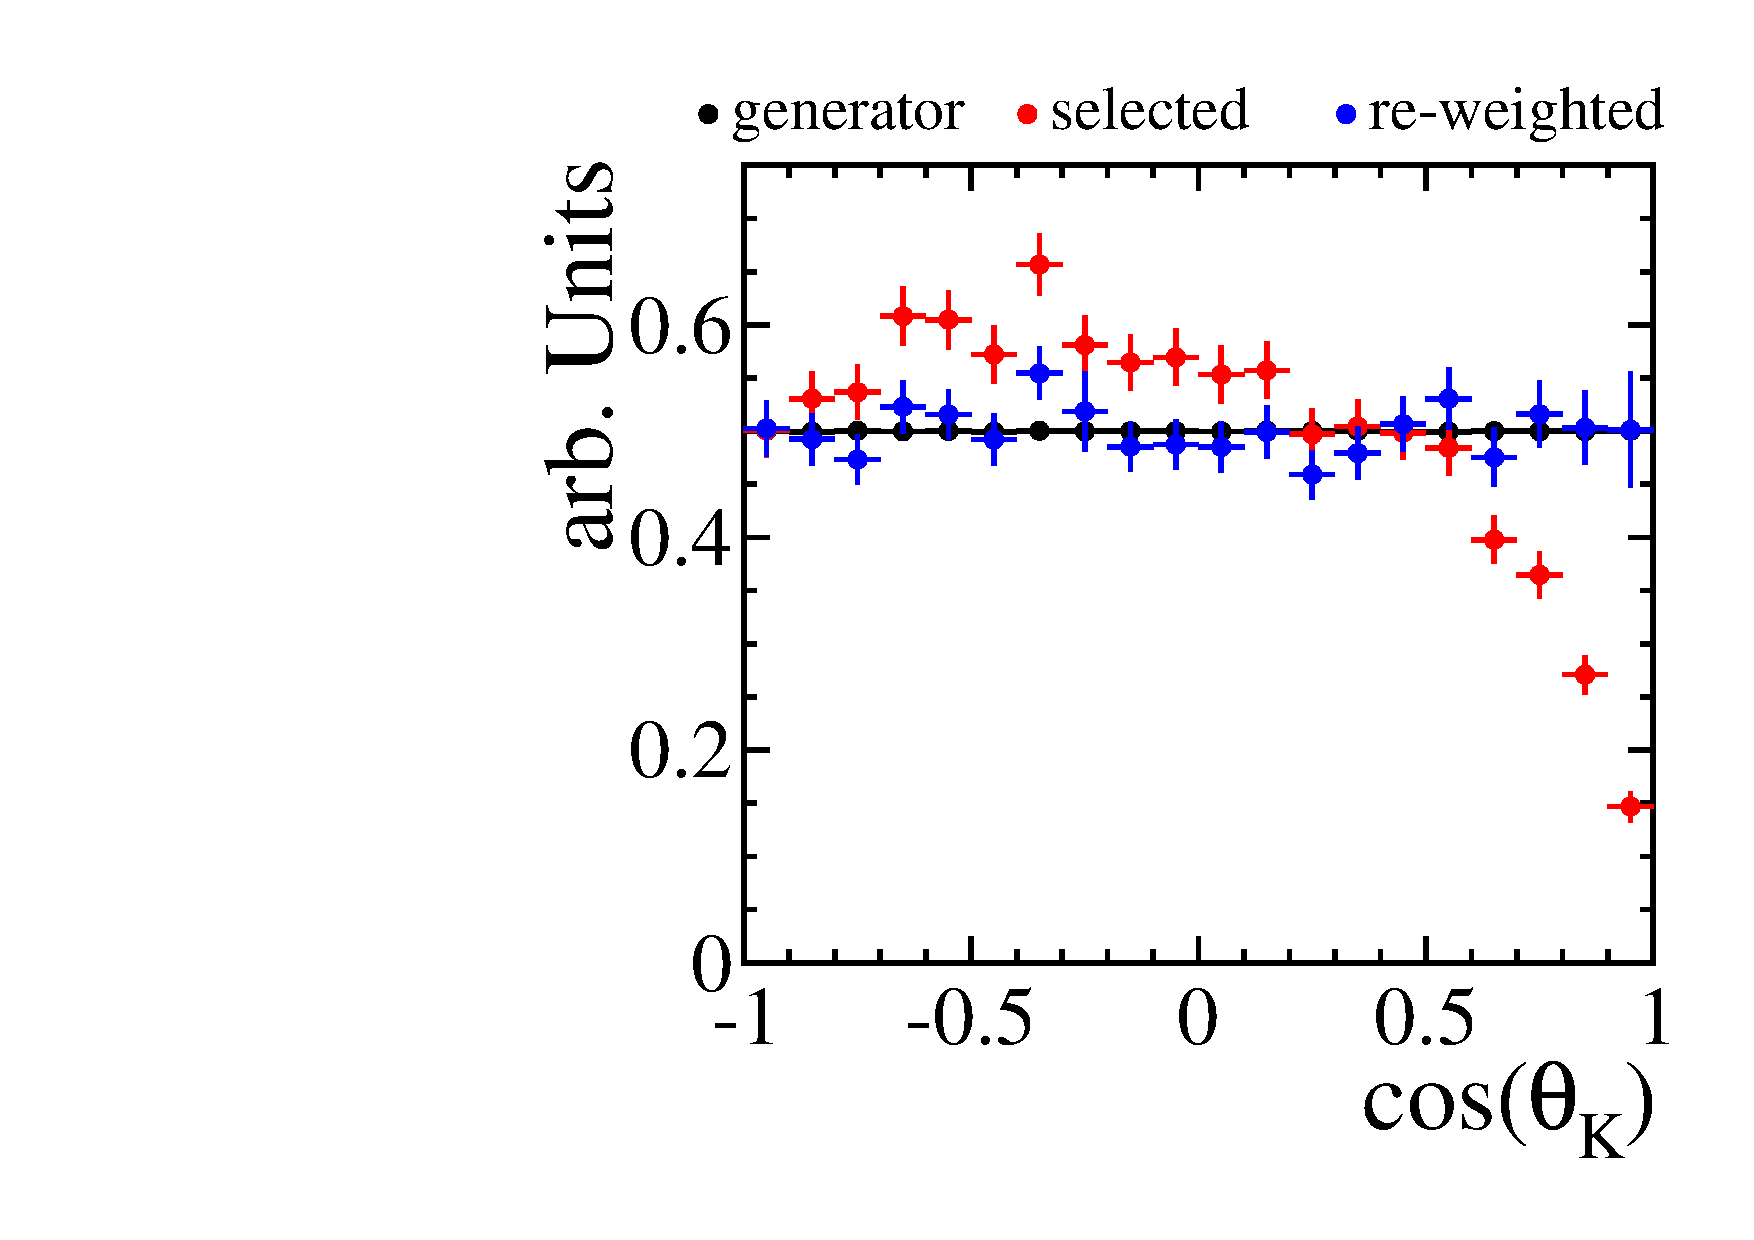
\includegraphics[width=0.48\columnwidth]{chapter5/figs/ac2/CorrectionsWithGen_ThetaK_new.pdf}}
\subfigure[]{\includegraphics[width=0.48\columnwidth]{chapter5/figs/ac2/CorrectionsWithGen_Phi_new.pdf}}
\caption{Generated (black), offline selected (red) and re-weighted (blue) events for  \BdToKstmm using the factorised acceptance correction method.~\label{fig:corrphsp2}}
\end{figure}
The compatibility between the re-weighted distribution and the distribution  of generator level events 
is good for both acceptance correction methods.


The k-nearest-neighbour method is by construction the most optimal acceptance correction method as it relies only on the accuracy of the simulation
 from which to calculate the efficiency. 
However, the dependence on the simulation statistics in regions of phase
space with low efficiency does not allow it to be used with larger
datasets. The factorised efficiency correction has for the 1.0\invfb
analysis a lower total systematic error. The statistical component from
the simulation sample size is much smaller but the assumption of
factorisation incurs an additional but still small systematic uncertainty.



\section{Angular analysis}
\label{sec:kstmm:pdf}

Each of the angular analyses were performed by simultaneously fitting a \PDF for the mass and the angular distribution 
to the data. % the extended maximum likelihood fit method.
%The \PDF used is a combination of a model for the the \Bd mass spectrum and the angular \PDF.
The simultaneous fit to the \Bd mass spectrum and to the angles ensures that the
 maximum information available is used to reduce the error on all of the angular observables.
It also ensures that the correlations are propagated correctly between the angular observables.
The total \PDF ($F$) is a combination of a model for the signal ($S$) and background ($B$) ,
each containing component \PDFs to describe the mass distribution and the angular distribution,
\begin{align}
F(\mB, \ctl, \ctk, \phi) = & f_{sig} \left( S_{i}(\mB) \times S_{i}(\ctl,\ctk,\phi) \right) \nonumber \\ 
&+ ( 1 - f_{sig} ) \left( B_{i}(\mB) \times B_{i}(\ctl,\ctk,\phi) \right) \, .
\end{align}
where $i$ indicates the model used for the first or second analysis.
The different components of the total \PDF are described in detail below.

The dataset is divided into seven bins of \qsq.
 There are six separate bins in the full \qsq range, detailed in Table~\ref{tbl:qsqbins}.
\begin{table}
\centering
\caption[ The \qsq binning scheme used in both angular analyses. ]
{ The \qsq binning scheme used in both angular analyses. 
The binning is analogous to the binning used in Ref~\cite{PhysRevLett.103.171801} including
 the  \qsq region of 1 to 6 \gevgevcccc .~\label{tbl:qsqbins} }
\begin{tabular}{|c|c|}
\hline
lower limit (\gevgevcccc)  & upper limit (\gevgevcccc) \\
\hline
0.1 & 2 \\
2 & 4.3 \\
4.3 & 8.68 \\
10.09 & 12.9 \\
14.18 & 16 \\
16 & 19 \\
\hline
1.0 & 6.0 \\
\hline
\end{tabular}
\end{table}
The binning is analogous to the binning used in Ref~\cite{PhysRevLett.103.171801} along with the
 region from $1 < \qsq < 6 \gevgevcccc $, which is a theoretically clean region where the observables are easily calculable.
The binning is chosen such that there is a bin below and above the point where \AFB is
 predicted to change sign in the Standard Model, and also with boundaries to avoid the \ccbar resonances.

\subsection{Mass model}
\label{sec:kstmm:massmodel}

Two different mass models were used to parametrise the \Bd signal invariant mass distribution.
The signal invariant mass model used to parametrise the \Bd invariant mass distribution in the first angular analysis was a double Gaussian function,
\begin{align}
\label{eq:totpdf}
S_{(1)}\left( \mkpimm ; \sigma_1, \sigma_2, \alpha, n \right) = & \, f \times G\left(  \mkpimm  ; m_B , \sigma_1 \right) \nonumber\\
& + \left(1-f\right) \times G\left(  \mkpimm ; m_B , \sigma_2\right) \, ,
\end{align}
where $f$ is the fraction of signal between each component and $\sigma_{1,2}$ are the different widths of each Gaussian component.
The signal mass model for the second angular analysis was an empirical model consisting of two Crystal Ball functions.
The Crystal Ball was a function developed to model the radiative 
tail from the \bbbar resonances~\cite{Skwarnicki:1986xj}.
It consists of a Gaussian distribution with an 
exponential tail and is expressed for a given mass ( \mkpimm ) as
\begin{equation}
\CB \left(  \mkpimm ; \mB , \sigma, \alpha, n \right) = N
\begin{cases}
  \exp{\left(\frac{-(\mkpimm - \mB )^2 }{2\sigma^2}\right)} 
 & \text{if} \,\, \mkpimm >  \alpha  \\
 \frac{\left(\frac{n}{\alpha^2}\right)^n}{\frac{\left(\mkpimm-\mB \right)}{\sigma} + \frac{n}{\alpha} - \alpha }
 & \text{if} \,\, \mkpimm\leq  \alpha
\end{cases}
\end{equation}
where $N$ is the signal normalisation, \mB is the nominal B mass, $\sigma$ is the Gaussian width and $n$ and $\alpha$ are the tail parameters.
Here the Crystal Ball function is used as an empirical formula to describe tails in the \Bd mass spectrum from resolution effects.
The parameters for the \Bd mass signal shape are assumed to be equivalent for both Crystal Ball functions except for the widths,
\begin{align}
S_{(2)}\left( \mkpimm ; \sigma_1, \sigma_2, \alpha, n \right) = & 
\, f \, \CB\left(  \mkpimm  ; m_B , \sigma_1, \alpha, n \right) \nonumber\\
& + \left(1-f\right) \times \CB\left(  \mkpimm ; m_B , \sigma_2, a, n \right) \ .
\end{align}

The shape of the signal mass model for both analyses is taken from fits to the \BdToJpsiKstar invariant mass spectrum. 
Due to the high statistics of \BdToJpsiKstar in the data, it is necessary to include an 
 additional contribution from the suppressed \BsToJpsiKstar mode.
The decay \BsToJpsiKstar is suppressed by a factor of \fd\Vtd/\Vts\fs compared to \BdToJpsiKstar.
The model used for the \BsToJpsiKstar is identical to the model for the \BdToJpsiKstar except for the central 
mass value and shares all of it's parameters with the \BdToJpsiKstar model. 
The only remaining free parameter is the relative normalisation between the two contributions.
There is a relative factor
\begin{align}
\frac{n_{\Bd}}{n_{\Bs}} =  0.007\pm0.002 \, ,
\end{align}
which is applied as a Gaussian constraint on the overall size of the \BsToJpsiKstar contribution.

The model for the background contribution to the \mkpimm spectrum for both analyses is the same. This is an exponential function,
\begin{align}
B_{(1,2)}\left(\mkpimm;\lambda\right) = N_B \exp{\left(-\lambda\mkpimm\right)} \, ,
\end{align}
where $\lambda$ is the decay constant for the exponential and $N_B$ is the normalisation of the background \PDF.

\subsection{Angular model}
\label{sec:kstmm:angularmodel}

The signal angular model for each of the analyses is a simplification of the full angular distribution for \BdToKstll 
as described in Sec.~\ref{sec:fullangdist}.
The angular distribution is integrated over one bin of \psq and integrated over each of the six bins of \qsq.
The signal model used in the 0.38\invfb angular analysis to measure \AFB and \FL is 
%a function of the angles \ctl and \ctk and integrated over $\phi$.% containing \AFB and \FL. 
%Integrating Eq.~\ref{eq:theo5d} over \psq and \varphi gives
\begin{align}
S_{(1)}(\ctl,\ctk) = & \frac{9}{16}   \Bigg( 2 \FL \ctksq ( 1 - \ctlsq )   \nonumber\\ 
& + \frac{1}{2} ( 1 - \FL ) ( 1 - \ctksq ) ( 1 + \ctlsq )  \nonumber\\
& +  \frac{4}{3} \AFB ( 1 - \ctksq ) \ctl   \Bigg) . 
\end{align}
The angular distribution for the 1.0\invfb angular analysis was extended to include angular observables dependent on \varphi. 
The distribution was simplified using the transformation described in Sec.~\ref{sec:fullangdist} and~\cite{Ksteepubnote}.
The analysis uses two parameterisations  of the angular distribution.
%, the first of which contains the regular angular observables from~\cite{AltmannshoferBall,Kruger:2005ep}.
The angular distribution for \AFB, \FL, \OS3 and \OS9 is given by
\begin{align}
\label{eq:theo4doriginal}
S_{(2a)}(\ctl,\ctk,\phiprime) =   \frac{9}{16\pi}  & \Bigg(  2 \FL \ctksq ( 1 - \ctlsq )  \nonumber \\ 
&  + \frac{1}{2} ( 1 - \FL ) ( 1 - \ctksq ) ( 1 + \ctlsq )  \nonumber \\
&  + \OS3 ( 1 - \ctksq ) (  1 - \ctlsq ) \cos2\phiprime  \nonumber \\
&  +  \frac{4}{3} \AFB ( 1 - \ctksq ) \ctl  \nonumber \\ 
&  + \OS9 ( 1 - \ctksq ) ( 1 - \ctlsq) \sin2\phiprime  \Bigg) . 
\end{align}
The re-parametrised angular distribution contains the transverse angular observables (\ATRe, \AT2, \ATIm) as described in Sec.~\ref{sec:kstmm:obs},
\begin{align}
\label{eq:theo4dreparam}
S_{(2b)}(\ctl,\ctk,\phiprime) =  \frac{9}{16\pi}  & \Bigg(  2 \FL \ctksq ( 1 - \ctlsq )  \nonumber \\ 
&  + \frac{1}{2} ( 1 - \FL ) ( 1 - \ctksq ) ( 1 + \ctlsq )  \nonumber \\
&  + \frac{1}{2} ( 1 - \FL ) \AT2 ( 1 - \ctksq ) (  1 - \ctlsq ) \cos2\phiprime  \nonumber \\
& +  \frac{4}{3}  ( 1 - \FL ) \ATRe ( 1 - \ctksq ) \ctl  \nonumber \\ 
& +  ( 1 - \FL ) \ATIm ( 1 - \ctksq ) ( 1 - \ctlsq) \sin2\phiprime  \Bigg) . 
\end{align}
The angular distribution used to measure \OA9 uses the CP anti-symmetric definition of \varphi where the sign changes
for \Bd and \Bdb decays as given in Sec~\ref{sec:kstmm:obs}.
The signal angular distribution is a function of \phiprimecp,
\begin{align}
\label{eq:theo4dphi}
S_{(2c)}(\ctl,\ctk,\phiprimecp) =   \frac{9}{16\pi}  & \Bigg(  2 \FL \ctksq ( 1 - \ctlsq )  \nonumber \\ 
&  + \frac{1}{2} ( 1 - \FL ) ( 1 - \ctksq ) ( 1 + \ctlsq )  \nonumber \\
&  + \OA3 ( 1 - \ctksq ) (  1 - \ctlsq ) \cos2\phiprimecp  \nonumber \\
&  +  \frac{4}{3} \AFB ( 1 - \ctksq ) \ctl  \nonumber \\ 
&  + \OA9 ( 1 - \ctksq ) ( 1 - \ctlsq) \sin2\phiprimecp  \Bigg) . 
\end{align}

The model for the background in each of the angles is equivalent for both angular analyses.
The background \PDF is an $n^{\text{th}}$ order Chebychev polynomial of the first kind for each angle,
\begin{align}
T_{n}(x) = \cos\left(n\arccos(x)\right) \, .
\end{align}
The total background angular \PDF is factorised into each of the angles,
\begin{align}
B(\mkpimm) = P`^{bkg}_{n}(\ctl, \ctk, \phiprime) = P_{n}^{L}(\ctl) \times P_{n}^{K}(\ctk) \times P_{n}^{P}\phiprime) \, .
\end{align}
The assumption that the background angular distribution factorises was tested using the point-to-point dissimilarity test~\cite{Williams:2010vh}.
The probability of the test statistic having a value less than the test statistic of the data was 25\%.
This value is entirely compatible with the assumption that the background factorises into the three angles.

\subsection{Result extraction}
\label{sec:kstmm:resextraction}

The signal \PDF is fitted to the data by performing an unbinned maximum-log-likelihood fit to the data,
minimising
\begin{align}
 - \log \mathcal{L} = \sum_{i}^{N}  \omega_i F(\mkpimm^i, \ctl^i, \ctk^i, \phi^i,  \vec{p} , \vec{O} ) ,
\end{align}
where $F$ is the total \PDF described in Eq.~\ref{eq:totpdf}. % which in terms of the \kpimm invariant mass and angles of each of the candidates.
The set of parameters for the signal and background mass models are $\vec{p}$, while $\vec{O}$ is the set of angular observables.
Each of the data candidates is weighted for acceptance as described in Section~\ref{sec:kstmm:ac}.
These weights distort the shape of the likelihood such that the errors extracted from the standard NLL minimisation are not 
guaranteed to be the true errors.
In each angular analysis, two different techniques were used to extract the likelihood minima and a better estimate of the error from the likelihood function.
In the 0.38\invfb analysis, the profile likelihood was calculated and the error determined from the two-dimensional 68\% confidence interval in both \AFB and \FL.
For the 1.0\invfb analysis, the errors were extracted in a Frequentist manner using the Feldman-Cousins (FC) technique~\cite{PhysRevD.57.3873}.

The FC technique maps out the likelihood for an observable, allowing the size of the confidence intervals for a given observable to be calculated. 
For an observable of interest in a given set of parameters, the ratio between the likelihood calculated with all parameters free $(\mathcal{L}_0)$ and the likelihood calculated with the observable fixed is calculated $(\mathcal{L}_1)$.
The ratio between these likelihood ($R_{data}$) is obtained for the result obtained from data, and for a large ensemble of toy datasets ($R_i$).
The fraction of $R_i < R_{data}$ ($f_R$) is proportional to the probability of the data result being the most optimum solution in the phase space of the parameters.
This fraction is calculated for a range of values for the observable and the 68\% confidence limits on the observable are calculated from the points where the $f_R<0.68$.

The results of the angular fits along with the calculated confidence limits are shown in Section~\ref{sec:kstmm:res}.



\section{Systematic uncertainties}
\label{sec:kstmm:sys}

Systematic effects which may affect the angular analysis are considered if there is an effect on 
the \kpimm invariant mass distribution, the \qsq spectrum or the angular distributions.
These include the acceptance correction method and the model for the \Bd mass spectrum.
There are three main categories of sources of systematic uncertainty, listed in order of importance
\begin{itemize}
\item Any systematic bias originating from the acceptance correction method.
\item The uncertainty on the data-simulation corrections used in the acceptance correction.
%\item The uncertainty on the acceptance correction due to the limited simulation events in the high \qsq region.
\item The uncertainty on the exact parametrisation of the \Bd mass spectrum and the use of polynomials to model the angular background.
\end{itemize}
All these effects were considered for both analyses but the exact size and specific systematic effects arising from the 
data-simulation corrections and acceptance method differ between the two analyses.
An additional source of systematic uncertainty was considered for the 1.0\invfb analysis from possible peaking backgrounds.
%This is due to the improved understanding of the detector after data-taking in 2011 was completed and the different methods used.


\subsection{Systematic contributions for the 0.38\invfb analysis}

The dominant systematic for the 0.38\invfb analysis comes from the acceptance correction, with other systematic contributions 
originating from the data-simulation corrections and a minor contribution from the model used for the \Bd mass distribution.

\subsubsection{Acceptance correction}

The systematic uncertainty from the acceptance correction method comes from the choice of the radius of the hyperspheroid.
The size of the possible bias was tested by using a smaller radius (0.01) and a larger radius (0.03) then the one chosen (0.02) to select events. 
Apart from the difference in the overall statistical error on the acceptance correction weight, no significant difference was found in the absolute efficiency.
The estimates of the systematic uncertainty arising from the various data-simulation corrections were propagated 
to give an overall uncertainty for the weight value given to each event.

In order to explore possible extreme systematic variations, two methods of altering the angular analysis were tested.
Firstly, the acceptance correction was ignored and the central values of \AFB and \FL 
 were found to move less than the statistical uncertainty on the observable. 
Secondly, the background model was assumed to be flat in the \ctl and \ctk to similar effect.
These extreme changes are not propagated to the final systematic uncertainty.

The systematic error on the observables is around $\approx30\%$ of the final statistical error.
%This contributes an $\approx3-4\%$ addition to the error in quadrature.
When added in quadrature to the statistical error, this only makes the total error (3-4)\% larger.
This is with the exception of the highest \qsq bin where 
the low simulation statistics leads to the total error being 10\% larger than the statistical error.


\subsubsection{Data-simulation corrections}

A conservative estimate of the uncertainty based on smearing the IP of the simulated tracks was tested by using the unsmeared tracks.
This can change the efficiency to select the events and the calculated angles.
%The gives an overall change to the total efficiency of \textcolor{red}{XX} and a change in the angular distribution of \textcolor{red}{YY}`.
A conservative estimate of the uncertainty associated with applying the correction for the hadron particle identification
 was evaluated by using the simulated values instead of the data-derived values.
This estimate gives a change in the absolute efficiency of around 20\% but does not change the angular distributions.
This estimate of the systematic uncertainty for the relative efficiency of the muon identification was obtained by changing the relative efficiency by one standard deviation.
The weight applied to the simulation is shifted down by $1\sigma$ for $p_\mu < 10\gevc$ and upwards for $p_\mu>10\gevc$.
A similar procedure is used to gain an estimate of the relative tracking efficiency but changing the weight applied for track momenta above and below 20\gev.
The effect of these changes on the measurement of the differential branching fraction is much smaller as it cancels out in the normalisation to \BdToJpsiKstar to first order.

\subsubsection{Mass model}

The systematic uncertainty associated with the model of the \Bd mass spectrum is evaluated by
 replacing the double Gaussian function with a double Crystal Ball function.
This tests the degree to which the tails of the Gaussian distribution are correctly modelled.
The systematic uncertainty associated with the background model is checked by using a linear function instead of an exponential function.
This is because the upper mass sideband may contain unknown background which can be incorrectly modelled by using a falling exponential.
The systematic uncertainty associated with using a polynomial to model the angular background is checked by
using a template function for the background, taken from a fit to the \Bd upper mass sideband, i.e. events with \mB of greater then 5400\mevmevcccc.
This ensures that the background model is free of any signal contribution but assumes that the high mass background is entirely combinatorial 
and the angular distribution is equivalent under the signal peak and in the high mass region.


\subsection{Systematic contributions in the 1.0\invfb analysis}

The contributions to the systematic uncertainty on the angular analysis of 1.0\invfb come from the 
the event selection, the model for the \Bd invariant mass and the acceptance correction.
The dominant effect comes from both the acceptance correction and the data-simulation corrections.
Tables of the size of the contribution from each of the possible sources of systematic uncertainty are given in Appendix~\ref{app:kstmm:systematics}.

\subsubsection{ Acceptance Correction}


The systematic uncertainty on the acceptance correction method was estimated by testing the addition
 of both factorisable effects, testing the addition of  non-factorisable effects and by using a different \qsq binning scheme.
The systematic uncertainty associated with factorisable effects was tested by changing the 
acceptance correction weight by a factorisable function that increases the weight at extreme values of 
\ctl and \ctk,
\begin{align}
\omega_i \to \omega_i \times ( 1 + \alpha \ctl^2 ) \times ( 1 + \alpha \ctk^2 ) .
\end{align}
The value of $\alpha$ was chosen to give a 10\% increase in the weight values at the extremities of the 
angular distribution. 
The estimate includes any mis-modelling of the efficiency in such a way that it will maximally affect the angular distribution.
The systematic uncertainty associated with non-factorisable effects was tested as described in Sec.~\ref{sec:kstmm:facac:nonfac}.
A non-factorisable effect of 10\% is used to provide an estimate of any hidden systematic effect because this is the maximum value that the 
acceptance correction is insensitive to.
The estimates of the systematic uncertainty from the acceptance correction are the dominant contribution to the total systematic error.


\subsubsection{Data-simulation corrections}

An estimate of the systematic uncertainty of each of the data-simulation corrections was evaluated for each of the different corrections.
The systematic uncertainty on the trigger efficiency is estimated by applying a weight of $\pm3\%$ to events with a muon of momentum less than 10\gev.
This comes from an estimate of the L0 trigger efficiency~\cite{Aaij:2012me}.
The systematic uncertainty on the relative tracking efficiency correction is changed twice. 
The relative tracking efficiency correction is shifted firstly down by one $\sigma$ for tracks below 20\gev and up by one $\sigma$ for tracks above 20\gev
 and secondly in the opposite direction.
This correction is chosen to reflect the possibility of a systematic mis-modelling of low momentum tracks and
to reflect the relatively easier reconstruction of high momentum tracks.
The relative efficiency for the muon identification is systematically shifted using the same method as the
relative tracking efficiency, but for muons with momentum above and below 10\gevc.
A possible source of systematic uncertainty from changing the particle identification for hadrons comes from the binning scheme used to calculate the new \dll values from data.
The effect of the binning scheme is tested twice by drawing \dll values from bins higher or lower for events close to the edge of the bin boundary.

In order to introduce a very conservative source of systematic uncertainty all hadrons with a momentum of less than
 3\gevc were removed from the sample of phase space simulated events.
The effect of this cut on the weight distribution as a function of \ctk and the effect on the re-weighted phase 
space simulated events is shown in Fig~\ref{fig:kstmm:sys:hadronp}.
\begin{figure}[tbp]
\centering
%\subfigure[]{\includegraphics[width=0.48\columnwidth]{chapter5/figs/sys/validation_weight_ctk_hadronpcut.pdf}}
%\subfigure[]{
\includegraphics[width=0.48\columnwidth]{chapter5/figs/sys/validation_weight_ctk_hadronpcut_new.pdf}
%}
\caption[  The effect of the removal of all hadrons of $p<3\gevc$ from the phase space simulation used in the acceptance correction.  ]
{ The effect of the removal of all hadrons of $p<3\gevc$ from the phase space simulation used in the acceptance correction. 
%The effect on a re-weighted phase space sample is shown in (a) where 
It is possible to see the artificially higher weights at high values of \ctk. 
%The effect on the weight values on the data sample is shown in (b). 
~\label{fig:kstmm:sys:hadronp} }
\end{figure}
%The estimate of the systematic uncertainty from this cut is not propagated to the final uncertainty because it is not a realistic .

\subsubsection{Mass Model}

There is a systematic effect from using the same mass model for the multiple different \qsq bins.
The widths of the two Crystal Ball functions used for the signal mass model are checked using 
corrected simulated \BdToKstmm data. The width is found to vary within errors to $\pm5\%$ and
both widths in the signal mass model are varied by this amount to compensate for this.

The systematic uncertainty on the parametrisation of the angular background is estimated by using a 
constant background as opposed to a $2^{\text{nd}}$ order Chebychev polynomial.
This has no significant impact on the values of the angular observables.

\subsubsection{Event Selection}

The two sources of possible systematic uncertainty from the event selection are from the 
consideration of peaking backgrounds and from the treatment of multiple candidates.
Peaking background decays such as \Bs\to\Kstarz\mumu and \Bs\to\varphi\mumu are difficult to account
for in the angular fit because the angular distribution of the decay products is not well known.
A conservative estimate of the contribution from these decays is assumed by assigning a
5\% systematic to the events that have $\AFB=\pm1$, $\FL=0,1$.
This method gives a total estimate of the systematic uncertainty from peaking backgrounds of approximately 2\%.

The treatment of multiple candidates is systematically accounted for by removing all events with multiple 
candidates.
The fraction of events with multiple candidates is between 1-2\% and consists mainly of \ktopi swapped candidates.
This has no impact on the final values for the angular observables.

\subsubsection{Tables of systematic uncertainties}




\section{Results}
\label{sec:kstmm:res}

The results for the angular analysis of \BdToKstmm for .38\invfb and 1.0\invfb of data collected at \lhcb are presented below.
A measurement of the differential branching fraction of \BdToKstmm was obtained by fitting
 the invariant mass distribution of selected candidates in each \qsq bin and normalising to \BdToJpsiKstar. 

\subsection{Angular analysis of 0.38\invfb of data}

The invariant mass distribution of the selected \BdToKstmm candidates in the data is shown in Fig.~\ref{fig:res1massfit}.
\begin{figure}[tbp]
\centering
\includegraphics[scale=0.33]{chapter5/figs/results1/mass_fit_full.pdf}
\caption[The fit to the \mkpimm invariant mass distribution of selected \BdToKstmm candidates from 0.37\invfb.]
{The fit to the \mkpimm invariant mass distribution of selected \BdToKstmm candidates from 0.37\invfb.
 The fit to the mass distribution gives an estimate of $337\pm21$ signal events. ~\label{fig:res1massfit}}
\end{figure}
The fit gives an estimate of $337\pm21$ signal events with a background of $97\pm6$ events.
The measured values of \AFB, \FL and the differential branching fraction of \BdToKstmm are shown in Fig.~\ref{fig:kstmm:res1}.
%along with a theoretical prediction from Ref.~\cite{Bobeth:2011gi}. 
\begin{figure}[tbp]
\centering
\subfigure[]{\includegraphics[scale=0.33]{chapter5/figs/results1/plot_AFB1.pdf}}
\subfigure[]{\includegraphics[scale=0.33]{chapter5/figs/results1/plot_FL1.pdf}}
\subfigure[]{\includegraphics[scale=0.33]{chapter5/figs/results1/plot_Width1.pdf}}
\caption[  The final results from the angular analysis of \BdToKstmm at \lhcb using 0.38\invpb of data collected in 2011 at 7 \tev. ]
{The final results from the angular analysis of \BdToKstmm at \lhcb using 0.38\invpb of data collected in 2011 at 7 \tev. 
Values for \AFB, \FL and the differential branching fraction are extracted in the six different bins of \qsq.
The Standard Model prediction is from~\cite{Bobeth:2011gi}
~\label{fig:kstmm:res1}}
\end{figure}
The central values for the angular observables along with the statistical and systematic errors are given in Table~\ref{table:kstmm:res1}.
\begin{table}[tbp]
\centering
\caption[ The central values and statistical plus systematic uncertainties
 for $A_{FB}$, $F_{L}$ and  $d{\BF}/dq^{2}$ for the 0.38\invfb angular analysis.   ]
{The central values and statistical plus systematic uncertainties
 for $A_{FB}$, $F_{L}$ and  $d{\BF}/dq^{2}$ for the 0.38\invfb angular analysis. 
The first, asymmetric, set of errors is given by the Bayesian error estimate, 
with a prior that the points sit within the physical region. 
The second error is the systematic error on $A_{FB}$, $F_{L}$ and the branching fraction.
\label{table:kstmm:res1}
}
\vspace{5mm}
\begin{tabular}{|c|c|c|c|}
\hline
$\qsq (\gevgevcccc) $ & \AFB & \FL & $d\BF/d\qsq$ ($\times10^{-7} \gev^{-2} c^{4}$)  \\  \hline
$0.10 < q^{2} < 2.00$ & $-0.15^{+0.20}_{-0.20}\pm 0.06$ & $0.00^{+0.13}_{-0.00}\pm 0.02$ & $0.61 \pm 0.12\pm 0.06$ \\
$2.00 < q^{2} < 4.30$ & $+0.05^{+0.16}_{-0.20}\pm 0.04$ & $0.77^{+0.15}_{-0.15} \pm 0.03$ & $0.34 \pm 0.09\pm 0.02$ \\ 
$4.30 < q^{2} < 8.68$ & $+0.27^{+0.06}_{-0.08}\pm 0.02$ & $0.60^{+0.06}_{-0.07} \pm 0.01$ & $0.69 \pm 0.08\pm 0.05$ \\ 
$10.09 < q^{2} < 12.86$ & $+0.27^{+0.11}_{-0.13}\pm 0.02 $ & $0.41^{+0.11}_{-0.11} \pm 0.03$ & $0.55 \pm 0.09\pm 0.07$ \\ 
$14.18 < q^{2} < 16.00$ &  $+0.47^{+0.06}_{-0.08}\pm 0.03$ & $0.37^{+0.09}_{-0.09}\pm 0.05$ & $0.63 \pm 0.11\pm 0.05$ \\ 
$16.00 < q^{2} < 19.00$ & $+0.16^{+0.11}_{-0.13}\pm 0.06$ & $0.26^{+0.10}_{-0.08}\pm 0.03$ & $0.50 \pm 0.08\pm 0.05$ \\
$1.00 < q^{2} < 6.00$ & $-0.06^{+0.13}_{-0.14}\pm 0.04$ & $0.55^{+0.10}_{-0.10}\pm 0.03$ & $0.42 \pm 0.06\pm 0.03$ \\
\hline
\end{tabular}
\end{table}
All of the values for the angular observables lie within the physical limits of \AFB and \FL (Section~\ref{sec:kstmm:obs}) except for the values for the
 $14.18<\qsq<16\gev^2$ bin.
The statistical errors for the physically valid \AFB and \FL values are given by the Bayesian error estimate with a prior that the points sit within the physical region. 
To extract a physical value for the  $14.18<\qsq<16\gev^2$ bin, the lowest value of the likelihood was taken and the errors obtained by integrating 
the likelihood to reach one $\sigma$ coverage.
These were the most precise measurements of the angular observables at the time of publication.


\subsection{Analysis of 1.0\invfb of data}

%The results of the angular analysis of \BdToKstmm at \lhcb using 1.0\invfb of data collected in 2011 are presented below.
The invariant mass distribution of selected \BdToKstmm candidates is shown in Fig.~\ref{fig:res2massfit}  
and there are an estimated $900\pm34$ signal candidates in 1.0\invfb of data. 
\begin{figure}[tbp]
\centering
\includegraphics[scale=0.33]{chapter5/figs/results2/KstarMuMuFit_q2low_0_1_q2high_19.pdf}
\caption[ The fit to invariant mass distribution of selected \BdToKstmm candidates from 1.0\invfb of data.  ]
{The fit to invariant mass distribution of selected \BdToKstmm candidates from 1.0\invfb of data.
The fit gives and estimate of $900\pm34$ candidates.~\label{fig:res2massfit}}
\end{figure}
The results for seven angular observables are presented in Table~\ref{table:kstmm:res2}.
The values for the differential branching fraction are presented in Table~\ref{table:kstmm:dbr2}.
\begin{table}[tbp]
\centering
\caption[Fraction of longitudinal polarisation of the \Kstarz, \FL, 
dimuon system forward backward asymmetry, \AFB, and the angular observables 
\OS3, \OS9 and \OA9 from the \BdToKstmm decay in six bins of \qsq.   ]
{Fraction of longitudinal polarisation of the \Kstarz, \FL, 
dimuon system forward backward asymmetry, \AFB, and the angular observables 
\OS3, \OS9 and \OA9 from the \BdToKstmm decay in six bins of \qsq. 
The lower table includes the transverse observables \ATRe and \AT2 
that are thought to have reduced form factor uncertainties. Results are also presented
 in the $1 < \qsq < 6\gevgevcccc$ range where theoretical uncertainties are 
best controlled.  \label{table:kstmm:res2}}
\begin{tabular}{|c|c|c|c|c|} 
\hline
\qsq $(\gevgevcccc)$ & \FL & \AFB & \OS3 & \OS9 \\
\hline
$0.10 - 2.00$ & $0.36\,^{+0.11}_{-0.10}\,^{+0.05}_{-0.03}$ & $-0.02\,^{+0.13}_{-0.12}\,^{+0.03}_{-0.00}$ & $-0.05\,^{+0.09}_{-0.10}\,^{+0.01}_{-0.01}$ & $\phantom{-}0.06\,^{+0.10}_{-0.10}\,^{+0.01}_{-0.00}$ \\
$2.00 - 4.30$ & $0.74\,^{+0.01}_{-0.12}\,^{+0.02}_{-0.02}$ & $-0.20\,^{+0.08}_{-0.08}\,^{+0.02}_{-0.01}$ & $-0.04\,^{+0.09}_{-0.08}\,^{+0.01}_{-0.01}$ & $-0.03\,^{+0.11}_{-0.04}\,^{+0.01}_{-0.01}$ \\
$4.30 - 8.68$ & $0.55\,^{+0.08}_{-0.07}\,^{+0.03}_{-0.03}$ & $\phantom{-}0.16\,^{+0.05}_{-0.06}\,^{+0.01}_{-0.02}$ & $\phantom{-}0.07\,^{+0.07}_{-0.08}\,^{+0.01}_{-0.01}$ & $\phantom{-}0.01\,^{+0.07}_{-0.08}\,^{+0.01}_{-0.00}$ \\
$10.09 - 12.86$ & $0.48\,^{+0.09}_{-0.07}\,^{+0.02}_{-0.04}$ & $\phantom{-}0.28\,^{+0.07}_{-0.06}\,^{+0.02}_{-0.02}$  & $-0.16\,^{+0.11}_{-0.08}\,^{+0.01}_{-0.01}$ & $-0.02\,^{+0.12}_{-0.11}\,^{+0.01}_{-0.01}$\\
$14.18 - 16.00$ & $0.33\,^{+0.08}_{-0.09}\,^{+0.02}_{-0.03}$ & $\phantom{-}0.51\,^{+0.08}_{-0.05}\,^{+0.02}_{-0.02}$ & $\phantom{-}0.03\,^{+0.09}_{-0.11}\,^{+0.02}_{-0.01}$ &  $\phantom{-}0.00\,^{+0.10}_{-0.09}\,^{+0.01}_{-0.01}$\\
$16.00 - 19.00$ & $0.38\,^{+0.10}_{-0.08}\,^{+0.03}_{-0.03}$ & $\phantom{-}0.30\,^{+0.08}_{-0.08}\,^{+0.01}_{-0.02}$ & $-0.22\,^{+0.11}_{-0.09}\,^{+0.02}_{-0.01}$ & $\phantom{-}0.06\,^{+0.11}_{-0.11}\,^{+0.01}_{-0.02}$ \\
\hline
$1.00 - 6.00$ & $0.65\,^{+0.08}_{-0.07}\,^{+0.03}_{-0.03}$ & $-0.15\,^{+0.07}_{-0.07}\,^{+0.02}_{-0.01}$ & $-0.03\,^{+0.08}_{-0.08}\,^{+0.01}_{-0.00}$ & $-0.05\,^{+0.08}_{-0.08}\,^{+0.01}_{-0.01}$ \\
\hline
\end{tabular}
\vspace{.5cm}\\
\begin{tabular}{|c|c|c|c|}
\hline
\qsq $(\gevgevcccc)$ & \OA9 & \AT2 & \ATRe \\
\hline
$0.10 - 2.00$ & $\phantom{-}0.12\,_{-0.09}^{+0.10}\,^{+0.01}_{-0.01}$ & $-0.16\,_{-0.31}^{+0.30}\,^{+0.03}_{-0.03}$ & $-0.04\,_{-0.24}^{+0.25}\,^{+0.03}_{-0.01}$ \\
$2.00 - 4.30$ & $\phantom{-}0.07\,_{-0.09}^{+0.12}\,^{+0.00}_{-0.01}$ & $-0.32\,_{-0.49}^{+0.65}\,^{+0.05}_{-0.04}$ & $-1.00\,_{-0.00}^{+0.15}\,^{+0.05}_{-0.01}$ \\
$4.30 - 8.68$ &	$-0.14\,_{-0.06}^{+0.07}\,^{+0.02}_{-0.01}$  & $\phantom{-}0.33\,_{-0.31}^{+0.30}\,^{+0.01}_{-0.05}$ & $\phantom{-}0.51\,_{-0.14}^{+0.15}\,^{+0.00}_{-0.05}$ \\
$10.09 - 12.86$ & $\phantom{-}0.00\,_{-0.11}^{+0.12}\,^{+0.01}_{-0.01}$ &	$-0.60\,_{-0.18}^{+0.41}\,^{+0.06}_{-0.02}$ & $\phantom{-}0.72\,_{-0.15}^{+0.14}\,^{+0.02}_{-0.03}$ \\
$14.18 - 16.00$ & $-0.07\,_{-0.08}^{+0.11}\,^{+0.02}_{-0.00}$ & $\phantom{-}0.07\,_{-0.28}^{+0.26}\,^{+0.00}_{-0.04}$ & $\phantom{-}1.00\,_{-0.05}^{+0.00}\,^{+0.01}_{-0.02}$ \\ 
$16.00 - 19.00$ & $\phantom{-}0.00\,_{-0.10}^{+0.11}\,^{+0.01}_{-0.01}$ & $-0.71\,_{-0.25}^{+0.34}\,^{+0.07}_{-0.04}$ & $\phantom{-}0.64\,_{-0.14}^{+0.14}\,^{+0.01}_{-0.03}$ \\ 
\hline
$1.00 - 6.00$ & $\phantom{-}0.02\,^{+0.08}_{-0.08}\,^{+0.01}_{-0.00}$ & $\phantom{-}0.15\,_{-0.42}^{+0.39}\,^{+0.04}_{-0.02}$ & $-0.57\,_{-0.22}^{+0.25}\,^{+0.03}_{-0.06}$\\ 
\hline
\end{tabular} 
\end{table}
\begin{table}
\centering
\caption[ Signal yield ($N_{\text{sig}}$) and differential branching fraction
 ($\deriv\BF/\deriv\qsq$) of the \decay{\Bz}{\Kstarz\mumu} decay.   ]
{Signal yield ($N_{\text{sig}}$) and differential branching fraction
 ($\deriv\BF/\deriv\qsq$) of the \decay{\Bz}{\Kstarz\mumu} decay in the six \qsq bins used in this analysis.
 Results are also presented in the $1 < \qsq < 6\gev^{2}/c^{4}$ range where theoretical uncertainties are best controlled. 
The final uncertainty on $\deriv\BF/\deriv\qsq$ comes from an estimate of the pollution from 
 \decay{\Bz}{\Kp\pim\mumu} in the $792 < m_{\Kp\pim} < 992\mevcc$ mass window. 
 \label{table:kstmm:dbr2}}
\begin{tabular}{|c|c|c|} 
\hline
\qsq $(\gev^{2}/c^{4})$ & $N_{\text{sig}}$ & $\deriv\BF/\deriv\qsq$ $(10^{-7} \gev^{-2} c^{4})$ \\
\hline
$0.10 - 2.00$ & $140 \pm 13$ & $0.61\pm 0.08 \pm 0.05 \,^{+0.00}_{-0.05}$ \\
$2.00 - 4.30$ & $\phantom{0}73 \pm 11$ & $0.30\pm 0.05 \pm 0.03 \,^{+0.00}_{-0.02}$ \\
$4.30 - 8.68$ & $271 \pm 19$ & $0.50\pm 0.05 \pm 0.04 \,^{+0.00}_{-0.04}$ \\
$10.09 - 12.86$ & $168 \pm 15$ & $0.43\pm 0.05 \pm 0.04 \,^{+0.00}_{-0.03}$ \\
$14.18 - 16.00$ & $115 \pm 12$ & $0.57\pm 0.07 \pm 0.04 \,^{+0.00}_{-0.05}$ \\
$16.00 - 19.00$ & $116 \pm 13$ & $0.42\pm 0.05 \pm 0.04 \,^{+0.00}_{-0.03}$ \\
\hline
$1.00 - 6.00$ & $197 \pm 17$ & $0.35\pm 0.04 \pm 0.04 \,^{+0.00}_{-0.03}$ \\
\hline
\end{tabular}
\end{table}
The results are also shown in Fig.~\ref{fig:kstmm:res2:norm}, Fig.~\ref{fig:kstmm:res2:reparam},
and Fig.~\ref{fig:kstmm:res2:a9dbr} along with the theoretical prediction from~\cite{Bobeth:2011gi} where available.
\begin{figure}[tbp]
\centering
\subfigure[]{\includegraphics[scale=0.31]{chapter5/figs/paper2/cAFB.pdf}}
\subfigure[]{\includegraphics[scale=0.31]{chapter5/figs/paper2/cFL.pdf}}
\subfigure[]{\includegraphics[scale=0.31]{chapter5/figs/paper2/cS3.pdf}}
\subfigure[]{\includegraphics[scale=0.31]{chapter5/figs/paper2/cS9.pdf}}
\caption[ The final results from the angular analysis of \BdToKstmm at \lhcb using 1.0\invfb of data collected in 2011 at 7 \tev.   ]
{The final results from the angular analysis of \BdToKstmm at \lhcb using 1.0\invfb of data collected in 2011 at 7 \tev. 
Values for the original observables are extracted in the six different bins of \qsq.
The Standard Model prediction is from~\cite{Bobeth:2011gi}.
~\label{fig:kstmm:res2:norm}}
\end{figure}
\begin{figure}[tbp]
\centering
\subfigure[]{\includegraphics[scale=0.31]{chapter5/figs/paper2/cATRE.pdf}}
%\subfigure[]{\includegraphics[scale=0.31]{chapter5/figs/results2/plot_ATI.pdf}}
\subfigure[]{\includegraphics[scale=0.31]{chapter5/figs/paper2/cAT2.pdf}}
\subfigure[]{\includegraphics[scale=0.31]{chapter5/figs/paper2/cA9.pdf}}
%\subfigure[]{\includegraphics[scale=0.31]{chapter5/figs/results2/plot_Width.pdf}}
\caption[ The final results from the angular analysis of \BdToKstmm at \lhcb using 1.0\invfb of data collected in 2011 at 7 \tev.   ]
{The final results from the angular analysis of \BdToKstmm at \lhcb using 1.0\invfb of data collected in 2011 at 7 \tev. 
Values for the the reparameterised observables and the CP asymmetric observable \OA9 are extracted in the six different bins of \qsq.
The Standard Model prediction is from~\cite{Bobeth:2011gi}.
~\label{fig:kstmm:res2:reparam}}
\end{figure}
\begin{figure}[tbp]
\centering
\subfigure[]{\includegraphics[scale=0.31]{chapter5/figs/paper2/cWidth.pdf}}
\caption[  The final results from the angular analysis of \BdToKstmm at \lhcb using 1.0\invfb of data collected in 2011 at 7 \tev.  ]
{The final results from the angular analysis of \BdToKstmm at \lhcb using 1.0\invfb of data collected in 2011 at 7 \tev. 
The differential branching fraction is extracted in the six different bins of \qsq.
The Standard Model prediction is from~\cite{Bobeth:2011gi}.
~\label{fig:kstmm:res2:a9dbr}}
\end{figure}













%\section{Interpretation}

The first angular analysis of \BdToKstmm has been interpreted both in context of placing constraints of the values of
the Wilson coefficients \C7, \C9 and \C10 ~\cite{Bobeth:2011nj}.
The constraints placed by measurements of electroweak penguin decays on the absolute 
magnitude of \C9 and \C10 are shown in Fig~\ref{fig:c9vsc10}.
\begin{figure}[tb]
\centering
\includegraphics[width=0.48\columnwidth]{chapter5/figs/theo/fig-constraints-c9-c10-all-all-all-contour.pdf}
\caption{ Constraints on the $|\C9 |$ v.s. $|\C10 |$ using the measurements of electroweak penguin decays
 available towards the end of 2011. Taken from Ref.~\cite{Bobeth:2011nj}.~\label{fig:c9vsc10} }
\end{figure}
A second interpretation of \BdToKstmm in the context of similar heavy flavour decays has also placed constraints on 
the values of the Wilson coefficients using the results from the first and second angular analyses respectively
~\cite{Altmannshofer:2011gn,Altmannshofer:2012az}.
It is possible to see that the measurements presented in this chapter provide some of the most stringent constraints on
 the values of the Wilson coefficients from \bquark\to\squark decays.




\section{Conclusions}

The angular analysis of \BdToKstmm  at \lhcb was performed on 
both 0.38\invfb and 1.0\invfb of data taken in 2011. 

Clean samples of \BdToKstmm candidates were selected using both a cut-based selection and a multi-variate algorithm. 
There were around 340 candidates in 0.38\invfb and 900 candidates in 1.0\invfb of data.
The first dataset is comparable to previous results from the \babar, \belle and \cdf 
and the second dataset is the largest sample of \BdToKstmm candidates at one experiment to date.

The candidates were corrected for the acceptance effect introduced by the reconstruction and selection by applying a weight to each event.
The first analysis used a $k$-nearest-neighbour method to calculate the efficiency to selected simulated events at a point in \ctl and \ctk.
This was an accurate calculation but the prevision and accuracy was limited by the number of simulated candidates in the regions of phase space with low efficiency.
The second analysis calculated the efficiency from a function fitted to each of the \ctl, \ctk and \varphi distributions independently.
This limitation of this method is that it assumes that the efficiency factorises into each dimension, which introduces additional sources of systematic uncertainty.
The method of weighting each of the \BdToKstmm candidate for their acceptance was chosen over the alternative method,
 of combining the signal model and a function for the efficiency, in order to minimise the number of free parameters in the final model. 	
This allowed measurement of the angular observables using the multi-dimensional angular distribution which fully incorporated the correlations between the angular observables.

The acceptance effect and the data-simulation corrections were the dominant sources of systematic uncertainty for both analyses. 
This is because the events with lowest efficiency, at extreme \ctl and high \ctk, have a large effect on the central value of \AFB and \FL.
This can be improved by a better understanding of the simulation and the efficiency to select \BdToKstmm candidates
 but the understanding of the efficiency in this region of phase space is a limitation on the accuracy of the measurement.

The first angular analysis obtained the worlds most precise measurements of the observables \AFB and \FL as well as measuring the differential branching fraction.
The second angular analysis improved the measurements of \AFB and \FL 
as well as measuring several new angular observables for the first time.
The measurements of \AFB and \FL from \lhcb along with the measurements from \babar, \belle and \cdf are shown in Figure~\ref{fig:res:comboexp}.
\begin{figure}[tbp]
\centering
\subfigure[]{\includegraphics[width=0.48\columnwidth]{chapter5/figs/plot_FLExp.pdf}}
\subfigure[]{\includegraphics[width=0.48\columnwidth]{chapter5/figs/plot_AFBExp.pdf}}
\caption{The measurements of the angular observables \FL and \AFB from \lhcb, \babar~\cite{Aubert:2007hz,Aubert:2008ju}, 
\belle~\cite{PhysRevLett.103.171801}  and \cdf~\cite{Aaltonen:2011cn,Aaltonen:2011ja} along with the theoretical prediction from Ref.~\cite{Bobeth:2011gi}. 
It is possible to see that the \lhcb results are the most precise and are compatible with the SM prediction.~\label{fig:res:comboexp}}
\end{figure}

The combination of these results, along with other radiative,
semi-leptonic and purely leptonic decays has enabled stringent limits to be set on the 
values for the Wilson coefficients \C7, \C9 and \C10 along with 
a high limit on the mass scale of any particle that contributes via
electroweak penguin diagrams~\cite{Bobeth:2011nj,Altmannshofer:2011gn,Altmannshofer:2012az}.
These constraints affect any new physics model that contains high mass particles with flavour couplings, 
providing a model-independent test of the mass scale of contributions from physics beyond the standard model.










\doublepage
\chapter{The effect of an S-wave on the angular analysis of \BdToKpill}
\label{chap:swave:theo}

\emph{This chapter is the work of the author except where referenced. This work was published in Ref~\cite{Blake:2012mb}. 
This work was based on Ref.~\cite{LHCb-CONF-2012-008} and uses different values for the angular observables than were measured in the previous chapter. 
This does not affect the conclusions of this chapter since the size of the bias comes from the size of the dilution factor coming from the \kpi S-wave contribution.
%The size of the S-wave contribution used is independant of the measured central values of the angular observables.
}

\section{Introduction}


The \lhcb detector is a single-arm forward spectrometer designed 
for precision measurements of particles containing \bquark quarks~\cite{Alves:2008zz}. 
It is one of the four main experiments at the Large Hadron Collider (\lhc) at the 
European Organisation for Nuclear Research (\cern) in Geneva, Switzerland.
In this chapter the \lhcb detector, its performance and its use to select \BdToKstmm events is shown.
The \lhcb detector is described in Section~\ref{sec:lhcb:det} detailing the sub-detector components
 required for measurements of \bsll decays. % (Section~\ref{sec:lhcb:sub}).
The trigger system used in the \lhcb detector is described in Section~\ref{sec:lhcb:trig} and 
an overview of the software used in \lhcb is given in Section~\ref{sec:lhcb:soft}.
The development of the trigger system used to select \BdToKstmm decays for the 2011 data-taking is presented in Section~\ref{sec:lhcb:trigdev} 
along with the final configuration of the \lhcb trigger system used throughout 2011.
%The high performance of the \lhcb detector throughout 2011 is presented in Section~\ref{sec:lhcb:perf}.

\subsection[CERN]{\cern}

\cern is an international organisation founded in 1954 in order to provide a 
politically neutral place to carry out research in nuclear and particle physics.
At the time of writing, \cern has 20 full member states and there are around ten thousand people associated with science at \cern.
Over the years that \cern has operated, it has contributed to the discovery of neutral currents~\cite{Hasert:1973ff}, 
the electroweak gauge bosons~\cite{Arnison:1983rp,Arnison:1983mk} and recently the Higgs boson~\cite{CMS:2012gu,ATLAS:2012gk}.
\cern is primarily home to the \lhc accelerator complex, which is a proton-proton ($pp$) collider with a circumference
 of 27\km at a depth of 100\m under the the French-Swiss border just outside Geneva.
The \lhc accelerator is built in the tunnel originally used for the \lep accelerator and ran at an energy of 
\sqs=7\tev in 2011.
The injection chain  for the \lhc consists of one linear accelerator and three synchrotrons as shown in Fig.~\ref{fig:lhccomplex}. 
\begin{figure}[tbp]
\centering
\includegraphics[width=0.48\columnwidth]{chapter3/figs/cern.pdf}
\caption[The \lhc ring.]{A illustration of the the \lhc accelerator complex showing each of the stages in the injection chain 
 for the \lhc ring along with the four main experiments on the \lhc ring~\cite{Lefevre:1092437}. ~\label{fig:lhccomplex} }
\end{figure}
It starts with a linear accelerator which accelerates the protons from rest to 50\mev. 
The synchrotrons increase the beam energy and refine the proton bunches to a configuration suitable for the \lhc. 
Firstly the Proton Synchrotron Booster (PSB) takes the beam from 50\mev to 1.5\gev at which point the 
beam enters the Proton Synchrotron (PS) where the beam energy is increased to 25\gev. 
The beam is then transferred to the Super Proton Synchrotron (SPS) which increases the energy to 450\gev
 before injecting the protons into the \lhc. 
The \lhc accelerates the proton bunches from injection energy at 450\gev to the final collision energy, which was 3.5\tev per beam in 2011 and 4\tev per beam in 2012.
Consolidation upgrades of the \lhc to take place in 2013 and 2014 are expected to increase this collision energy to the design energy of 7\tev per beam.
During operation in 2011-12 there were 1380 proton bunches per beam with a bunch spacing of 50\ns.
There are four main experiments on the \lhc ring, two general purpose detectors (\atlas and \cms), 
along with a heavy-ion experiment (\alice) and a dedicated B-physics experiment (\lhcb).

At the \lhcb interaction point the instantaneous luminosity of the colliding proton bunches 
 is constant at around $\lum\approx3\times10^{32}\cm^2\sec^{-1}$. 
This is significantly below the  \lhc  luminosity, which in 2011 reached over $\lum\approx1\times10^{33}\cm^2\squark^{-1}$.
This luminosity was chosen so that the number of interactions per proton bunch crossing ($\mu$) 
stayed uniform throughout the period of proton collisions for each `fill' of the \lhc.
This ensures that the environment is consistent and has a low multiplicity for reconstruction of \B mesons 
but that there is still a sufficient number of \B meson decays of interest for a given number of collisions.

The production of \bbbar pairs in $pp$ interactions is governed predominantly 
by gluon fusion, $gg\to\bbbar$.
The collision of partons of unequal energy and a momentum boost along the direction of the collision results in \bbbar pairs 
that are produced at small angles to the beam axis.
The angular distribution of \bbbar production is shown in Fig.~\ref{fig:lhcb:bbbar}.
\begin{figure}[tbp]
\centering
\includegraphics[width=0.48\columnwidth]{chapter3/figs/angular.pdf}
\caption[ $b\bar{b}$ production at the LHC ]{The angular distribution of \bbbar pairs in terms of the polar angle from the beam axis.
The \bbbar pairs are largely produced within a very small opening angle hence the development of \lhcb as a forward spectrometer
~\cite{Alves:2008zz}.~\label{fig:lhcb:bbbar} }
\end{figure}
The \bbbar cross section at \sqs=7\tev is 75\mub within the \lhcb acceptance~\cite{LHCb-PAPER-2010-002}. 
%This corresponds to around $10^7$ \bbbar pairs produced in the 2011 year of data-taking.
In total the experiment recorded an integrated luminosity of 1.0\invfb in 2011 that could be used for further analysis.
The increase in integrated luminosity throughout the year can be seen in Fig.~\ref{fig:lhcb:intlumi} along with the technical stops
 and periods of machine development.
\begin{figure}
\centering
\includegraphics[width=0.66\columnwidth]{chapter3/figs/2011IntegratedLumiLHCbTime_NoPie.png}
\caption{The integrated luminosity recorded by \lhcb during 2011~\cite{OpsPlots}.~\label{fig:lhcb:intlumi} }
\end{figure}


\section{Theoretical formalism of the \psq spectrum}
\label{sec:swave:theo}

The \BdToKpill angular distribution can be expressed for multiple S-wave states 
as described in Section~\ref{sec:fullangdist} and Ref.~\cite{Lu:2011jm}.
For \kpi masses below  
$1200\mev$,  the %it can be seen from the previous section that
contribution to the amplitudes from the higher $\Kstarz$ states is 
small enough that it can be ignored.
In order to understand the S-wave contribution to the \BdToKpill angular distribution
 close to the $\Kstarz(892)$ so only the $J=0,1$ terms in
the sums of Eq.~\ref{eq:amp} were considered.

The S-wave contribution to these amplitudes only enters in the amplitude $\mathcal{A}_{0}$, 
\begin{align}
\label{eq:amps1}
\mathcal{A}_{H0} &= \sqrt{\frac{1}{4\pi}} A_{0H0} + \sqrt{\frac{3}{4\pi}} A_{1H0} \ctk    \\
\mathcal{A}_{H||} &= \sqrt{\frac{3}{8\pi}} A_{1H||} \stk  \\
\mathcal{A}_{H\bot} &= \sqrt{\frac{3}{8\pi}} A_{1H\bot} \stk   
\end{align}
where the spherical harmonics are expanded, leaving the phase space factor, 
the propagator and the matrix element as part of the spin-dependent amplitudes
\begin{equation}
\label{eq:amps2}
\begin{split}
A_{0,H,0} &\propto \rho(\psq,\qsq) \times M_{0,H,0} (\qsq) \times  P_0(\psq) , \\
A_{1,H,0} &\propto  \rho(\psq,\qsq) \times  M_{1,H,0} (\qsq) \times  P_1(\psq) , \\
A_{1,H,\bot} &\propto  \rho(\psq,\qsq)  \times M_{1,H,\bot} (\qsq) \times  P_1(\psq) , \\
A_{1,H,||} &\propto  \rho(\psq,\qsq) \times M_{1,H,||} (\qsq) \times P_1(\psq) ,  
\end{split}
\end{equation}
where the first index denotes the spin. 
The normalisation from the three-body phase space factor is described in more detail below.

\subsection{Phase space factors}
\label{sec:swave:phasespace}

The phase space for the four-body decay \BdToKpill can be described by three three-body phase space factors
\begin{align}
\rho(\Bd\to(\kpi)(\ellell)) \times \rho((\kpi)\to\kaon\pion) \times \rho((\ellell)\to\ellp\ellm) \, .
\end{align}
The three-body phase space factor is
\begin{align}
\rho(a \to b c ) = \left(\frac{\sqrt{ \lambda ( a, b , c ) }}{8\pi a^2}\right)^{2J+1}
\end{align}
where $\lambda(a,b,c) = \left(a^2+b^2+c^2\right)^2-4b^2c^2$ is the triangle function and $J$ is
 the difference in spin of $a$ and $b$. 
%The \qsq-dependent phase space factor is assumed to be fixed and the combination of \qsq and \psq dependence is not considered in this chapter.
The phase space for \BdToKpill as a function of \psq and \qsq is given in Fig.~\ref{fig:phasespace}. 
\begin{figure}[tb]
\centering
\includegraphics[width=0.48\columnwidth]{chapter6/figs/test_phasespace_psq_qsq.pdf}
\caption[ The phase space for \BdToKpill as a function of \psq and \qsq.   ]
{ The phase space for \BdToKpill as a function of \psq and \qsq. 
The kinematic edge for the high mass \Kstarz states is clearly seen. ~\label{fig:phasespace} }
\end{figure}
The region of S-wave and P-wave interference is mainly at \psq values below $1200^2\mevmevcccc$
 where there is a small reduction in phase space at high \qsq.

\subsection{Propagator functions}
\label{sec:swave:propfunctions}

The propagator for the P-wave is described by a relativistic Breit-Wigner distribution with the amplitude given by
\begin{align}
\label{eq:rbw}
P_1(\psq) = \frac{ m_{\Kstarzo} \Gamma_{\Kstarzo}(\psq)}{ m_{\Kstarzo}^2 - \psq + i \  m_{\Kstarzo} \Gamma_{\Kstarzo}(\psq)} 
\end{align}
where  $m_{\Kstarzo}$ is the resonant mass and 
\begin{align}
\Gamma_{\Kstarzo}(\psq) = \Gamma_{\Kstarzo}^0 \left( \frac{ t }{t_0} \right)^{2J+1} \left( \frac{ m_{\Kstarzo} }{ p } \right) \frac{ B\left(tR_P\right) }{ B\left(t_0R_P\right) }
\end{align}
the running width. Here $t$ is the \Kp momentum in the rest frame of the \kpi system and $t_0$ is t evaluated at the \kpi pole mass.
$B$ is the Blatt-Weisskopf damping factor~\cite{Blatt:628052} with a radius $R_P$.
For P-wave the value of $R_P$ is taken to be $3.0\gev^{-1}$  (from Ref~\cite{Aubert:2008aa}). 
The amplitude can be defined in terms of a phase ($\delta$) through the substitution
\begin{align}
\cot \delta = \frac{  \psq - m_{\Kstarzo}^2 }{  \Gamma_{m_{\Kstarzo}}(\psq) m_{\Kstarzo} }
\end{align}
to give the polar form of the relativistic Breit-Wigner propagator 
\begin{align}
P_1(\psq) =   \frac{1}{\cot\delta - i } 
\end{align}
The LASS parametrisation of the S-wave~\cite{Aston:179353} 
can be used to describe a generic \kpi S-wave.  
In this parametrisation, the S-wave propagator is defined as 
\begin{align}
\label{eq:lass}
P_0(\psq) = \frac{p}{t} \left( \frac{1 }{ \cot\delta_B - i } + e^{2i\delta_B}( \frac{1}{\cot\delta_R - i }) \right)
\end{align}
where the first term is an empirical term from inelastic scattering and the second term is
 the resonant contribution with a phase factor to retain unitarity.
The first phase factor is defined as
\begin{align}
\cot\delta_B = \frac{1}{ta} + \frac{1}{2}rt ,
\end{align}
where $r$ and $a$ are free parameters and $t$ is defined previously,
while the second phase factor describes the $\Kstarzz(1430)$
 through 
\begin{align}
\cot\delta_R = \frac{ \psq - m_{\mathrm{S}}^2 }{ \Gamma_{\mathrm{S}}(\psq) m_{\mathrm{S}}  }.
\end{align}
Here, $m_{\mathrm{S}}$ is the S-wave pole mass and $\Gamma_{\mathrm{S}}$ is the 
running width using the pole mass of the $\Kstarzz(1430)$.
The overall strong phase shift between the results from the LASS scattering experiment and 
measured values for \Bd\to\jpsi\kpi has been found to be consistent with $\pi$~\cite{Aubert:2004cp}. 
The parameters for the \psq spectrum used are given in Table~\ref{tbl:params}.
\begin{table}[tb]
\centering
\caption[ Parameters of the \kpi resonances used to generate toy data sets.    ]
{Parameters of the \kpi resonances used to generate toy data sets. The \Kstar masses and widths 
are taken from Ref.~\cite{PDG2012} and the \Kstarzo Blatt-Weisskopf radius and 
the LASS parameters are taken from Ref.~\cite{Aubert:2008aa}~\label{tbl:params}}
\begin{tabular}{|c|c|c|c|c|c|c|}
\hline
State. & mass & $\Gamma$ & R & $r$ & $a$ & $ \delta_{\mathrm{J}} $ \\
  & (\mev) & $(\mev)$ & ($\gev)^{-1}$ & $(\gev)^{-1}$ & $(\gev)^{-1}$ &  \\
\hline
\Kstarzz & $ 1425  \pm 50 $ & $ 270 \pm 80 $ & $1.0$ & $1.94$ & $1.73$ &  $\pi$ \\
\Kstarzo & $ 894.94  \pm 0.22$ & $ 48.7 \pm 0.8 $ & $3.0$  & \  & \ & 0  \\
\Kstarzt & $ 1432.4  \pm 1.3$ & $ 109 \pm 5 $ & $1.5$  & \  & \ & 0  \\
\hline
\end{tabular}
\end{table} 

\subsection{Angular coefficients}
The angular terms modified by the inclusion of the S-wave are $I_{1,2,4,5,7,8}$ and  
the complete set of angular terms expressed in terms of the spin-dependent amplitudes
are
%Some important features from the angular coefficiencts can by understoof by examination of $I_1^c$, given as
\begin{align}
\label{eq:angularcoeff1}
I_1^c &=  \frac{1}{4\pi} |A_{0L0}|^2 + \frac{3}{4\pi} |A_{1L0}|^2\ctksq + 2 \frac{\sqrt{3}}{4\pi} |A_{0L0}||A_{1L0}|\cos\delta_{0,0}^L \ctk + (L\to R) \frac{}{}  \nonumber \\
I_1^s &= \frac{3}{4} \frac{3}{8\pi} \left( |A_{1L||}|^2 + |A_{1L\bot}|^2 + (L\to R) \right) \frac{}{}\stksq \nonumber   \\
I_2^c &= - I_1^c , \qquad \, I_2^s = \frac{1}{3} I_1^s \nonumber\\ 
I_3 &= \frac{1}{2}  \frac{3}{8\pi}  \left( |A_{1L\bot}|^2 - |A_{1L||}|^2 + (L\to R) \right) \stksq  \frac{}{}\nonumber\\
I_4 &= \frac{1}{\sqrt{2}} \left[  \frac{1}{4\pi}\sqrt{\frac{3}{2}}\Re( A_{0L0}A_{1L||}^{*}) \cos\delta_{0,||}^L \stk  \right. \frac{}{} \nonumber\\
      &+ \left. \frac{3}{4\pi}\sqrt{\frac{1}{2}}\Re( A_{1L0}A_{1L||}^{*})  \stk \ctk  + ( L \to R )  \right] \frac{}{}\nonumber \\
I_5 &= \frac{1}{\sqrt{2}} \left[  \frac{1}{4\pi}\sqrt{\frac{3}{2}}\Re( A_{0L0}A_{1L\bot}^{*}) \cos\delta_{0,\bot}^L \stk  \right. \frac{}{} \nonumber\\
    &+  \left.  \frac{3}{4\pi}\sqrt{\frac{1}{2}}\Re( A_{1L0}A_{1L\bot}^{*})  \stk \ctk  - ( L \to R )  \right] \frac{}{} \\
I_6 &= 2  \frac{3}{8\pi} \left( \Re(A_{1L||}A_{1L\bot}^{*}) - (L\to R) \right) \stksq \frac{}{} \nonumber  \\
I_7 &= \frac{1}{\sqrt{2}} \left[  \frac{1}{4\pi}\sqrt{\frac{3}{2}}\Im( A_{0L0}A_{1L||}^{*}) \cos\delta_{0,||}^L \stk \right. \frac{}{}  \nonumber\\ 
    & + \left.   \frac{3}{4\pi}\sqrt{\frac{1}{2}}\Im( A_{1L0}A_{1L||}^{*})  \stk \ctk   - ( L \to R )  \right] \frac{}{} \nonumber \displaybreak[1]  \\
I_8 &= \frac{1}{\sqrt{2}} \left[  \frac{1}{4\pi}\sqrt{\frac{3}{2}}\Im( A_{0L0}A_{1L\bot}^{*}) \cos\delta_{0,\bot}^L \stk \right. \frac{}{} \nonumber\\
 &  + \left.    \frac{3}{4\pi}\sqrt{\frac{1}{2}}\Im( A_{1L0}A_{1L\bot}^{*})   \stk \ctk  + ( L \to R )  \right]  \frac{}{} \nonumber \\
I_9 &=    \frac{3}{8\pi} \left(  \Im(A_{1L||}A_{1L\bot}^{*}) + (L\to R) \right) \stksq \frac{}{}\nonumber
\end{align}
The interference term of $I_1$ shows how this parametrisation includes the
 strong phase difference between the S- and P-wave state. 
The left handed part of the interference term for $I_1$ can be written as 
\begin{align}
2 |A_{0L0}||A_{1L0}|\cos\delta_{0,0}^L \propto 2\, |M_{0,L,0}||P_0(\psq)||M_{1,L,0}||P_1(\psq)| \cos( \delta_{0,0}^L ) 
\end{align}
where 
\begin{align}
 \delta_{0,0}^L =  \delta_{M_{0L0}} + \delta_{P_0} - \delta_{M_{1L0}} - \delta_{P_1}  .
\end{align}
where $\delta_{M_{JL0}}$ is the phase of the  longitudinal matrix element and 
$\delta_{P_J}$ is the phase of the propagator.
The phases in the interference terms for $I_{4,5,7,8}$ can be similarly defined.
For real matrix elements,~i.e.~nearly true in the Standard Model, the phases are 
equal for both handed interference terms $\delta^L = \delta^R$.
The phase difference between the S-wave and the P-wave propagators can be 
expressed as a single strong phase, $\delta_{\mathrm{S}}$.



\subsection{The \psq spectrum for \BdToKpill}

The \psq spectrum for the  \BdToKpill angular distribution can
 be calculated by summing over the S- and P-waves and integrating 
out the \ctl, \ctk and $\phi$ dependence. This is illustrated in 
Fig.~\ref{fig:psqat6}
\begin{figure}[tb]
\centering
\includegraphics[width=0.66\textwidth]{chapter6/figs/calc_psq_branch_frac_logy.pdf}
\caption[  An illustration of the \psq spectrum for the P-wave (dashed) and the S-wave (dotted).    ]
{ An illustration of the \psq spectrum for the P-wave (dashed) and the S-wave (dotted). 
The total distribution from both states  is the 
solid line. The values were calculated at $q^2 = 6 \gev^2$ by
 integrating out the angular distribution of \BdToKpill using equal 
matrix elements for each state. The S-wave fraction here is 16\% between $800<p<1000 \mev$~\label{fig:psqat6} } 
\end{figure}
where the matrix elements from 
Refs.~\cite{Egede:2008uy,Egede:2010zc} at a \qsq value of $6\gev^2$ are used. 
Here the S-wave amplitude is assumed to be equivalent to the longitudinal P-wave amplitude.
The S-wave fraction in the $800 < p < 1000\mev$ window around the P-wave 
is calculated to be 16\% when using this approximation.
The size of the S-wave fraction, the P-wave fraction and the interference fraction w.r.t the total branching fraction
are given in Fig.~\ref{fig:fracat6}.
\begin{figure}[tb]
\centering
\subfigure[]{\includegraphics[width=0.48\textwidth]{chapter6/figs/calc_psq_branch_frac_S.pdf}}
\subfigure[]{\includegraphics[width=0.48\textwidth]{chapter6/figs/calc_psq_branch_frac_P.pdf}}
\subfigure[]{\includegraphics[width=0.48\textwidth]{chapter6/figs/calc_psq_branch_frac_int.pdf}}
\caption[  An illustration of the size of the S-wave, P-wave and S$\leftrightarrow$P-wave
 interference fractions with respect to the total branching fraction. ]
{ An illustration of the size of the S-wave, P-wave and S$\leftrightarrow$P-wave
 interference fractions with respect to the total branching fraction. 
The values were calculated at $q^2 = 6 \gev^2$ by
 integrating out the angular distribution of \BdToKpill using equal 
matrix elements for each state.~\label{fig:fracat6} } 
\end{figure}
As will be seen later there are no interference terms left in the angular distribution after the integral
 over \ctk.




\section{Angular observables}
\label{sec:kstmm:obs}

The contributions from the Wilson coefficients defined above
 can be measured by measuring the transversity amplitudes
 through an angular analysis of the \BdToKstll angular distribution.
Direct measurements of the transversity amplitudes are dependent on the values of the form factors
 which have a significant theoretical uncertainty.
To mitigate these uncertainties and allow measurements of the Wilson coefficients, angular observables
can be constructed from the transversity amplitudes that are independent of the two heavy-to-light form factors.
Many angular observables have been proposed for the decay 
\BdToKstll~\cite{Kruger:2005ep,AltmannshoferBall,Egede:2008uy,Bobeth:2010wg,Matias:2012xw}. 
These observables are combinations of the amplitudes which both minimise the uncertainty from the form factors 
and maximise the contribution from new physics models. 
So far the forward-backward asymmetry (\AFB), the fraction of the \Kstarz longitudinal polarisation (\FL ) 
and two combinations of the transverse amplitudes (\AT2 and \AIm ) have been 
measured~\cite{Aaltonen:2011cn,Aubert:2007hz,Aaltonen:2011ja,Aubert:2008ju,PhysRevLett.103.171801}.

\subsection{P-wave observables}

These observables are constructed from combinations of amplitudes and
are normalised to the sum of amplitudes for the P-wave state, given as 
\begin{align}
|A_{10}|^2 + |A_{1||}|^2 + |A_{1\bot}|^2 \, ,
\end{align}
where the generic combination of amplitudes $A_{Ji}A_{Ji}^{*}$ is defined for a spin $J$ and a polarisation (0,$||$,$\bot$) as
\begin{align}
\label{eq:ampsq}
A_{Ji} A_{Ji}^{*} &= A_{JiL} A_{JiL}^{*} + A_{JiR} A_{JiR}^{*} \, .
\end{align}
The forward-backward asymmetry of the dilepton system, \AFB, enters in the angular coefficient $I_6$ and
is defined in terms of the amplitudes as
\begin{align}
\label{eq:theoafb}
\AFB(\qsq) &= \frac{3}{2} \frac{  \Re(A_{1L||}A_{1L\bot}^{*}) - 
\Re(A_{1R||}A_{1R\bot}^{*})}{|A_{10}|^2 + |A_{1||}|^2 + |A_{1\bot}|^2 } \, .
\end{align}
In a similar way, \FL, \OS3 and \OS9 are defined as
\begin{equation}
\begin{split}
\FL(\qsq) &= \frac{  |A_{10}|^2 } {|A_{10}|^2 + |A_{1||}|^2 + |A_{1\bot}|^2} \\
\OS3 (\qsq) &= \frac{ |A_{1\bot}|^2 - |A_{1||}|^2 }{ |A_{10}|^2 + |A_{1||}|^2 + |A_{1\bot}|^2} \\
\OS9 (\qsq) &= \frac{  \Im(A_{1L||}A_{1L\bot}^{*}) - \Im(A_{1R||}A_{1R\bot}^{*}) }{|A_{10}|^2 + |A_{1||}|^2 + |A_{1\bot}|^2} 
\end{split}
\end{equation}
where \OS3 and \OS9 are related to the angular coefficients $I_3$ and $I_9$ respectively.
These theoretical observables are normalised to the sum of the P-wave amplitudes
and the factorisation of the amplitudes into matrix elements and the 
propagators removes the \psq dependence from these theoretical observables. 

In terms of the angular distribution, \AFB can also be expressed 
as the difference 
between the number of `forward-going' \mup and the number of 
`backward-going' \mup in the rest frame of the \Bd,
\begin{align}
\label{eq:expafb}
\left[ \int_0^1 - \int_{-1}^0 \right]  \text{d}\ctl
\frac{\text{d}\Gamma}{\text{d}\qsq \text{d}\ctl} / 
\frac{\text{d}\Gamma}{\text{d}\qsq} \, ,
\end{align}
which explains the name of the observable. 

\subsection{Transverse observables}
\label{sec:kstmm:reparam}

Angular observables which are normalised to only the transverse helicity amplitudes have
 been studied with the additional aim of reducing the theoretical uncertainties~\cite{Melikhov:1998cd,Kruger:2005ep}.
This is achieved by separating out the dependence on the  longitudinal amplitudes and their form factors from the calculation.
The main transverse observable is \AT2 which comes from the angular coefficient $I_3$,
\begin{align}
\AT2 (\qsq) &=  \frac{ |A_{1\bot}|^2 - |A_{1||}|^2  }{ |A_{1\bot}|^2 + |A_{1||}|^2 }  \, .
\end{align}
The observables associated with $I_6$ and $I_9$ can be similarly reparameterised~\cite{Becirevic:2011bp} 
 to give
\begin{equation}
\begin{split}
\ATRe(\qsq) &= \frac{ |A_{1\bot}|^2 - |A_{1||}|^2 }{ |A_{1||}|^2 + |A_{1\bot}|^2} \\
\ATIm(\qsq) &= \frac{  \Im(A_{1L||}A_{1L\bot}^{*}) \Im(A_{1R||}A_{1R\bot}^{*}) }{ |A_{1||}|^2 + |A_{1\bot}|^2} \, .
\end{split}
\end{equation}
These observables are correlated to $(1-\FL)$ when the the angular distribution is normalised to the sum of the P-wave amplitudes.

\subsection{\CP asymmetric angular observables}

Angular observables equivalent to \OS3 and \OS9 for the \CP antisymmetric angular distribution can by constructed
from the definition of $I_i - \bar{I}_i$.
Two \CP antisymmetric angular observables, \OA3 and \OA9 for the angular coefficients $I_3$ and $I_9$,
which can be compared to the \OS{i} angular observables 
\begin{align}
\OA3 &= \frac{1}{2} \frac{\left(I_3 - \bar{I}_3\right)}{ |A_{10}|^2 + |A_{1||}|^2 + |A_{1\bot}|^2} \, , \\
\OA9 &= \frac{1}{2} \frac{\left(I_9 - \bar{I}_9\right)}{ |A_{10}|^2 + |A_{1||}|^2 + |A_{1\bot}|^2}  \, .
\end{align}

\subsection{Relation to the Wilson coefficients}

Each of the observables is related to the Wilson coefficients through bi-linear combinations of the transversity amplitudes.
This means that there are terms proportional to the combinations $|\Ceff{9,10} \pm \Cpeff{9,10} |^2$ and $|\Ceff7 - \Cpeff7 |^2$.
Each of these terms is multiplied by the relevant \Kstarz form factors giving the \qsq dependence. 
This can be seen in the SM predictions for \AFB and \FL in Fig.~\ref{fig:otherexp}.







\section{Testing the effect of a \kpi S-wave}
\label{sec:swave:testing}

In an angular analysis of \BdToKpill, the S-wave can be considered to be 
a systematic effect that could bias the results of the angular observables.
The implications of this systematic effect are tested by generating toy 
Monte Carlo experiments and fitting the angular distribution to them.
The results of the fit to the observables are evaluated for multiple toy 
datasets.

The effect of the S-wave is evaluated for two different cases.
Firstly, the effect of S-wave interference  is examined as a function 
of the size of the dataset used.
The aim of this study is to explore the possibility of biases in any measurements to date and the
 possible implications on future measurements of \BdToKpill.
Datasets of sizes between 50 and 1000 events are tested.
For comparison, the results from Chapter~\ref{chap:kstmm} 
have between 20 and 200 signal events in the 6 different \qsq bins considered.
Second, the effect of different levels of S-wave contribution is examined. 
At present, the only information about the S-wave fraction is 
obtained by the measurement of \FS of approximately 7\% in the decay $\Bd\to\jpsi\kpi$
from~\cite{Aubert:2004cp} for the range $800 < p < 1000 \mev$. 
As the value may be different in \BdToKpill, we consider 
values of \FS in this region ranging from 1\% to 60\%. 
The fraction of the S-wave, \FS, is expected to have some \qsq dependence
 because of the \qsq dependence of the transverse P-wave amplitudes.

The parameters used to generate the toy datasets are summarised in 
Tables~\ref{tbl:params} and~\ref{tbl:obs}.
The values of the angular observables used  to generate toy Monte Carlo
 simulations are taken from the analysis of 1.0\invfb presented in~\cite{LHCb-CONF-2012-008}. %Section~\ref{sec:kstmm:results}.
Within errors, these measurements are compatible with the Standard Model prediction for \BdToKstll 
and the central value of the measurement is used.
The nominal magnitude  and phase difference of the S-wave contribution 
are taken from the angular analysis of \Bd\to\jpsi\kpi~\cite{Aubert:2004cp}.
The toy datasets are generated as samples of pure signal in order to test the
trend on the bias on the angular observables in the signal distribution that could be incurred from an increasing \kpi S-wave component.
As this is a phenomenological study, a background component is not included as this is not expected to affect the trends.
The correlation between the S-wave component and any possible background is expected to be small. This
expectation is based on the results presented in Table X of~\cite{LHCB-PAPER-2013-002} where the uncertainty in the background on the \Kp\Km S-wave component in
the \Bs\to\jpsi\varphi final state is evaluated and shown to be small.
\begin{table}[tb]
\caption[ Parameters used to generate toy datasets.   ]
{Parameters used to generate toy datasets. \AFB, \FL, \AT2 and \AIm
 are taken from ~\cite{LHCb-CONF-2012-008} %Section~\ref{sec:kstmm:results}  
 in the $1 < \qsq < 6~(\gev^2)$ bin. 
The \FS value is taken from Ref.~\cite{Aubert:2004cp}~\label{tbl:obs}}.
\centering
\begin{tabular}{|c|c|c|c|c|c|}
\hline
Obs.  & \AFB & \FL & \AT2 & \AIm  & \FS  \\
\hline
Value &$ -0.15 $ &$ 0.65$  & $ 0.03/(1-0.65)$ & $0.05$  & $0.07$  \\
\hline
\end{tabular}
\end{table}

The toy datasets are generated as a function of the
 \ctl, \ctk, $\phi$ and \psq using an accept/reject method.
 The PDF used is the angular distribution given in 
 Eq.~\ref{eq:theo5d}.
For each set of input parameters 1000 toy datasets were generated.
For each of these toy datasets, an unbinned log likelihood fit is 
performed that returns the best fit value of the observables 
and an estimate of their error.
The expected experimental resolution is obtained by plotting 
the best fit values of an observable for the ensemble of toy 
simulations as illustrated for \AFB in Fig.~\ref{fig:toyexample} (left).
 The pull value for an observable ($O$) is defined as 
\begin{align}
p_{O}^i= \frac{ O_{\text{fit}}^i - O_{\text{gen}}^i }{ \sigma_{O}^i }
\end{align}
where $\sigma_O^i$ is the estimated error on the fit to the observable $O^i$.
This distribution is seen in Fig.~\ref{fig:toyexample} (right). 
The mean and the width are extracted from a Gaussian fit.
For a well performing fit without bias, the pull distribution should 
have zero mean and unit width. 
A negative pull value implies that the result is underestimated 
and a positive pull value implies overestimation of the true observable.
\begin{figure}[tb]
\centering
\subfigure[]{\includegraphics[width=0.48\textwidth]{chapter6/figs/fit_result_test_afb_gen_val_plot_new.pdf}}
\subfigure[]{\includegraphics[width=0.48\textwidth]{chapter6/figs/fit_result_test_afb_gen_pull_plot_new.pdf}}
\subfigure[]{\includegraphics[width=0.48\textwidth]{chapter6/figs/fit_result_test_fl_gen_val_plot_new.pdf}}
\subfigure[]{\includegraphics[width=0.48\textwidth]{chapter6/figs/fit_result_test_fl_gen_pull_plot_new.pdf}}
\caption[  Distribution of the results and pull  
values for \AFB (a,b) and \FL (c,d) respectively 
for fits to 1000 toy simulations each containing 1000 events. ]
{Distribution of the results and pull 
values for \AFB (a,b) and \FL (c,d) respectively 
for fits to 1000 toy simulations each containing 1000 events.
The S-wave is ignored in these fits. The resolution obtained on \AFB is 
$0.026\pm0.001$. Since the S-wave is ignored there is a non-zero 
pull mean for both observables at $(0.26\pm0.02)$ and $(-0.65\pm0.02)$ respectively. 
The widths of the pull distribution are consistent with unity at 
 $(1.01\pm0.01)$ and $(0.99\pm0.01)$.~\label{fig:toyexample}}
\end{figure}



\section{The impact of ignoring the S-wave in an angular analysis of \BdToKstll}
\label{sec:swave:ignore}

The effect of ignoring or including a \kpi S-wave was tested as a function of dataset 
 size in order to find a minimum dataset at which the bias 
 from ignoring the S-wave contribution to the angular distribution when measuring the angular observables becomes significant.
Datasets were generated for sample sizes ranging from 50 to 
1000 events and analysed assuming a pure P-wave state. 
The results are shown in Fig.~\ref{fig:bias}. 
\begin{figure}[tb]
\centering
\subfigure[]{\includegraphics[width=0.48\textwidth]{chapter6/figs/fit_result_ds_gen_res.pdf}}
\subfigure[]{\includegraphics[width=0.48\textwidth]{chapter6/figs/fit_result_ds_gen_mean.pdf}}
\subfigure[]{\includegraphics[width=0.48\textwidth]{chapter6/figs/fit_result_ds_gen_width.pdf}}
\caption[ Resolution, pull mean and width of 
1000 toy datasets analysed as a pure P-wave state as a 
function of dataset size.    ]
{Resolution (a), pull mean (b) and pull width (c) of 
1000 toy datasets analysed as a pure P-wave state as a 
function of dataset size. It can be seen that the bias 
on the observable (non-zero pull mean) increases dramatically as the sample 
size increases. This is because the statistical error 
decreases increasing the sensitivity to the ignored S-wave 
contribution. The bias of \AFB is positive  
because \AFB is negative in the \qsq bin chosen. 
~\label{fig:bias}}
\end{figure}

From Eq.~\ref{eq:theo4d}, it can be seen that \AT2 
has a factor of (1-\FL) in front of it. The large 
value of \FL used to generated datasets is 
in turn causing \AT2 to have a much worse 
resolution than \AFB, \FL and \OS3 . There is 
significant bias (non-zero mean) of the pull distribution for all
 observables when the S-wave is ignored in the angular distribution for datasets 
 of more than 200 events. This corresponds to a 
 change of 0.2$\sigma$ in \FL for a dataset of 200 events.
The behaviour can be understood in terms of the $(1-\FS)$ 
factor in Eq.~\ref{eq:theo4d}. It gives an offset to the 
fitted values of the observables which are proportional 
to the value of $(1-\FS)$.

The angular fit was performed on toy 
datasets with an increasing S-wave contribution.
Datasets of 500 events were generated with a 
varying S-wave contribution in the narrow \psq
 mass window of ($800 < p < 1000 \mev$) 
 from no S-wave up to a \FS value of $0.4$. 
The resolution and the mean and width of the pull 
distribution for each of the four observables
 (\AFB, \FL, \AT2 , \OS3 ) were calculated and 
 the results are shown in Fig.~\ref{fig:fsval}.
\begin{figure}[tb]
\centering
\subfigure[]{\includegraphics[width=0.48\textwidth]{chapter6/figs/fit_result_fs_gen_res.pdf}}
\subfigure[]{\includegraphics[width=0.48\textwidth]{chapter6/figs/fit_result_fs_gen_mean.pdf}}
\subfigure[]{\includegraphics[width=0.48\textwidth]{chapter6/figs/fit_result_fs_gen_width.pdf}}
\caption[ The resolution, mean and width of the pull distribution 
of 1000 toy datasets analysed as a pure 
P-wave state as a function of the S-wave contribution.   ]
{The resolution (a) the mean (b) and the width (c) of the pull distribution
of 1000 toy datasets analysed as a pure 
P-wave state as a function of S-wave contribution. 
The resolution and the bias can be seen to increase with the size of the S-wave 
contribution in a linear fashion. ~\label{fig:fsval}}
\end{figure}
Significant bias is seen in the angular 
observables when the S-wave is ignored for an S-wave magnitude of greater than 5\%.
The linear increase in the bias 
is another consequence of the (1-\FS) factor in the angular distribution.



\section{Measuring the S-wave in \BdToKpill}
\label{sec:swave:measurement}

Obtaining unbiased values for the angular observables beyond the limits
 shown requires including the S-wave contribution in the angular model. % rather than ignoring it.
With the formalism developed in Section~\ref{sec:swave:theo}, three options are explored for measuring
it. The first option is to ignore the \psq dependence in the measured parameters and simply fit for
\psq-averaged values of \FS and \AS. The second option is to fit the \psq 
 line-shape simultaneously with the angular distribution.
This can be done in a small $p$ window between $800$ and $1000\mev$
or in the region from the lower kinematic threshold 
to $1200\mev$.
In all cases the datasets used to perform the 
studies are identical to those used in Sect. 5.1 
%The difference is in how the fit is performed.In each case, 
and the dataset and the S-wave sizes 
refer to the number of events in the smaller \psq window.

The angular distribution without \psq dependence is given in Eq.~\ref{eq:theo4dint}.
For each set of samples, the resolution and the mean 
and the width of the pull distribution of the angular observables are tested. 

The change in the resolution obtained on the angular observables 
for the three different methods of including the S-wave in the angular distribution
 (ignoring the \psq dependence, fitting a narrow \psq window and fitting a wide \psq window) 
is demonstrated by plotting the ratio with respect
to the resolution obtained when a single 
P-wave state is assumed.

The resolution and the mean of the pull distributions for the three different fit methods are shown
relative to the resolution and mean obtained using the assumption of a pure P-wave state. 
The ratio between the fit methods, including the S-wave in the angular distribution and 
assuming a P-wave state, as a function of dataset size
are shown in  Fig~\ref{fig:ratiods}.
\begin{figure}[tb]
\centering
\subfigure[\AFB]{\includegraphics[width=0.48\textwidth]{chapter6/figs/fit_result_ratio_ds_afb_res.pdf}}
\subfigure[\FL]{\includegraphics[width=0.48\textwidth]{chapter6/figs/fit_result_ratio_ds_fl_res.pdf}}
\subfigure[\AT2 ]{\includegraphics[width=0.48\textwidth]{chapter6/figs/fit_result_ratio_ds_at2_res.pdf}}
\subfigure[\AIm]{\includegraphics[width=0.48\textwidth]{chapter6/figs/fit_result_ratio_ds_aim_res.pdf}}
\caption[ Resolutions for three different methods to incorporate 
the S-wave relative to the resolution obtained when the S-wave is ignored.    ]
{Resolutions for three different methods to incorporate 
the S-wave relative to the resolution obtained when the S-wave is ignored. 
It can be seen that the best resolution is obtained when using the largest \psq window.
The original resolution is recovered to within 10\%. ~\label{fig:ratiods}}
\end{figure}
The pull mean for all three fit methods is shown in Fig~\ref{fig:combods}.
\begin{figure}[tb]
\centering
\subfigure[\AFB]{\includegraphics[width=0.48\textwidth]{chapter6/figs/fit_result_combo_ds_afb_mean.pdf}}
\subfigure[\FL]{\includegraphics[width=0.48\textwidth]{chapter6/figs/fit_result_combo_ds_fl_mean.pdf}}
\subfigure[\AT2 ]{\includegraphics[width=0.48\textwidth]{chapter6/figs/fit_result_combo_ds_at2_mean.pdf}}
\subfigure[\AIm]{\includegraphics[width=0.48\textwidth]{chapter6/figs/fit_result_combo_ds_aim_mean.pdf}}
\caption[ Pull mean for the three different  
methods to incorporate the S-wave and when the S-wave 
is ignored.      ]
{Pull mean for the three different  
methods to incorporate the S-wave and when the S-wave 
is ignored. There is a slight shift when the S-wave is 
included for datasets of less than 200 events but this is removed from  all the observables 
when the S-wave is included in the fit 
for datasets of over 500 events. ~\label{fig:combods}}
\end{figure}
The pull width for all three fit methods is shown in Fig~\ref{fig:combodswidth}.
\begin{figure}[tb]
\centering
\subfigure[\AFB]{\includegraphics[width=0.48\textwidth]{chapter6/figs/fit_result_combo_ds_afb_width.pdf}}
\subfigure[\FL]{\includegraphics[width=0.48\textwidth]{chapter6/figs/fit_result_combo_ds_fl_width.pdf}}
\subfigure[\AT2 ]{\includegraphics[width=0.48\textwidth]{chapter6/figs/fit_result_combo_ds_at2_width.pdf}}
\subfigure[\AIm]{\includegraphics[width=0.48\textwidth]{chapter6/figs/fit_result_combo_ds_aim_width.pdf}}
\caption[ Pull width for the three different  
methods to incorporate the S-wave and when the S-wave 
is ignored.  ]
{Pull width for the three different  
methods to incorporate the S-wave and when the S-wave 
is ignored. There is a slight shift when the S-wave is 
included for datasets of less than 200 events but this is removed from  all the observables 
when the S-wave is included in the fit 
for datasets of over 500 events. ~\label{fig:combodswidth}}
\end{figure}

For all observables, it can be seen that the resolution degrades when
the S-wave is included and the \psq dependence is ignored.  The
resolution degrades by a smaller amount when the \psq dependence is
included in a small bin and the original resolution is recovered to
within 10\% when using the large \psq range.  There are two effects
contributing to the improvement of the resolution. There are more
P-wave events in the larger range and the wider mass window allows for
the S-wave to be constrained by using the information from above and
below the P-wave resonance.  This results in the best resolution when
the S-wave is included in the angular distribution.

For all the observables, the pull mean approaches zero for datasets of
greater than 300 events implying that the bias present in the
observables when a pure P-wave state is assumed is removed when an S-wave is
included in the angular distribution. This means that the inclusion of
the S-wave component will be mandatory for all future experimental
analyses.


The ratio of the resolutions for the three different fit methods
as a function of increasing S-wave size is given in Fig.~\ref{fig:ratiofs}.
\begin{figure}[tb]
\centering
\subfigure[\AFB]{\includegraphics[width=0.48\textwidth]{chapter6/figs/fit_result_ratio_fs_afb_res.pdf}}
\subfigure[\FL]{\includegraphics[width=0.48\textwidth]{chapter6/figs/fit_result_ratio_fs_fl_res.pdf}}
\subfigure[\AT2 ]{\includegraphics[width=0.48\textwidth]{chapter6/figs/fit_result_ratio_fs_at2_res.pdf}}
\subfigure[\AIm]{\includegraphics[width=0.48\textwidth]{chapter6/figs/fit_result_ratio_fs_aim_res.pdf}}
\caption[  Resolutions for three different methods to incorporate 
the S-wave relative to the resolution obtained when the S-wave is ignored.   ]
{Resolutions for three different methods to incorporate 
the S-wave relative to the resolution obtained when the S-wave is ignored. 
It can be seen that the best resolution is obtained when using the largest \psq window.
The original resolution is recovered to within 10\%. ~\label{fig:ratiofs}}
\end{figure}
The pull mean  as a function of S-wave contribution 
for all three fit methods is shown in Fig.~\ref{fig:combofs}.
\begin{figure}[tb]
\centering
\subfigure[\AFB]{\includegraphics[width=0.48\textwidth]{chapter6/figs/fit_result_combo_fs_afb_mean.pdf}}
\subfigure[\FL]{\includegraphics[width=0.48\textwidth]{chapter6/figs/fit_result_combo_fs_fl_mean.pdf}}
\subfigure[\AT2 ]{\includegraphics[width=0.48\textwidth]{chapter6/figs/fit_result_combo_fs_at2_mean.pdf}}
\subfigure[\AIm]{\includegraphics[width=0.48\textwidth]{chapter6/figs/fit_result_combo_fs_aim_mean.pdf}}
\caption[ Pull mean for the three different  
methods to incorporate the S-wave and when the S-wave 
is ignored.    ]
{Pull mean for the three different  
methods to incorporate the S-wave and when the S-wave 
is ignored. There is a slight shift when the S-wave is 
included for datasets of less than 200 events but this is removed from  all the observables 
when the S-wave is included in the fit 
for datasets of over 500 events. ~\label{fig:combofs}}
\end{figure}
The pull width  as a function of S-wave contribution 
for all three fit methods is shown in Fig.~\ref{fig:combofswidth}.
\begin{figure}[tb]
\centering
\subfigure[\AFB]{\includegraphics[width=0.48\textwidth]{chapter6/figs/fit_result_combo_fs_afb_width.pdf}}
\subfigure[\FL]{\includegraphics[width=0.48\textwidth]{chapter6/figs/fit_result_combo_fs_fl_width.pdf}}
\subfigure[\AT2 ]{\includegraphics[width=0.48\textwidth]{chapter6/figs/fit_result_combo_fs_at2_width.pdf}}
\subfigure[\AIm]{\includegraphics[width=0.48\textwidth]{chapter6/figs/fit_result_combo_fs_aim_width.pdf}}
\caption[ Pull width for the three different  
methods to incorporate the S-wave and when the S-wave 
is ignored.    ]
{Pull width for the three different  
methods to incorporate the S-wave and when the S-wave 
is ignored. There is a slight shift when the S-wave is 
included for datasets of less than 200 events but this is removed from  all the observables 
when the S-wave is included in the fit 
for datasets of over 500 events. ~\label{fig:combofswidth}}
\end{figure}





\section{Systematic test}
\label{sec:swave:isobar}

The results shown in Figs.~\ref{fig:combods} and~\ref{fig:combofs} could
 have an implicit model dependence through the use of the LASS parametrisation to model the \psq spectrum.
 In order to understand the size of this effect, the measurements were repeated using an isobar
model to parametrise the \kpi S-wave as in Ref.~\cite{PhysRevLett.89.121801}.
In the isobar model the S-wave is described as a simple sum of functions for the $\Kstarzz(1430)$ 
and the $\kappa(800)$ along with a constant non-resonant term,
\begin{align}
T_I(\psq) &= N_{\kappa} \mathcal{F}_{\kappa}(\psq) \exp(\phi_{\kappa}) + N_S \mathcal{F}_S(\psq) \exp(\phi_S)  + NR
\end{align}
where $N_i$ is the normalisation for each contribution and $\phi_i$ is the phase of each contribution.
The $\Kstarzz(1430)$ is described by a relativistic Breit-Wigner function as in the LASS parametrisation,
\begin{align}
\mathcal{F}_S(\psq) &= \cot\delta_S = \frac{ \psq - m_{\mathrm{S}}^2 }{ \Gamma_{\mathrm{S}}(\psq) m_{\mathrm{S}}}.
\end{align}
and the $\kappa(800)$ is described similarly
\begin{align}
\mathcal{F}_{\kappa}(\psq) &= \cot\delta_{\kappa} = \frac{ \psq - m_{\kappa}^2 }{ \Gamma_{\kappa}(\psq) m_{\kappa}  }.
\end{align}
where the mass and width of the $\kappa(800)$ are taken from Ref.~\cite{PDG2012}.
The existence of the $\kappa(800)$ is under debate with no conclusive evidence.
The amplitude $T_I$ is normalised such that it has the same integral as the LASS amplitude ($T_S$) 
over the \psq range from threshold to an upper limit of 2.5\gevgevcccc. 
This limit is chosen to encompass most of resonant $\Kstarzz(1430)$.
The \psq spectrum of the combined P wave and the two S-wave models is shown in Fig.~\ref{fig:spwave:isobar}.
\begin{figure}[tb]
\centering
\includegraphics[width=0.66\textwidth]{chapter6/figs/calc_isobar_psq_branch_frac_logy.pdf}
\caption{ An illustration of the \psq spectrum for the P-wave (solid) and the
 isobar S-wave (dashed) and the LASS S-wave (dash-dotted) and the D-wave (dotted). 
~\label{fig:spwave:isobar} } 
\end{figure}

The model-dependence of the \psq spectrum was tested by generating events where an isobar model was used for 
the S-wave contribution and fitting the angular distribution using the LASS parametrisation.
The relative resolution between the results obtained when generating with the 
LASS parametrisation and the results obtained when generating with an isobar model
are shown in Fig.~\ref{fig:ratio:isobar}.
\begin{figure}[tb]
\centering
\subfigure[\AFB]{\includegraphics[width=0.48\textwidth]{chapter6/figs/fit_result_ratio_ds_isobar_afb_res.pdf}}
\subfigure[\FL]{\includegraphics[width=0.48\textwidth]{chapter6/figs/fit_result_ratio_ds_isobar_fl_res.pdf}}
\subfigure[\AT2 ]{\includegraphics[width=0.48\textwidth]{chapter6/figs/fit_result_ratio_ds_isobar_at2_res.pdf}}
\subfigure[\AIm]{\includegraphics[width=0.48\textwidth]{chapter6/figs/fit_result_ratio_ds_isobar_aim_res.pdf}}
\caption[ Resolutions for three different methods to incorporate 
the S-wave relative to the resolution obtained when the S-wave is ignored.   ]
{Resolutions for three different methods to incorporate 
the S-wave relative to the resolution obtained when the S-wave is ignored. 
The S-wave has been generated using an isobar model. ~\label{fig:ratio:isobar}}
\end{figure}
The bias on the central values of the angular observables when the S-wave is ignored
as a function of the size of the dataset is shown in Fig.~\ref{fig:combods:isobar}.
\begin{figure}[tb]
\centering
\subfigure[\AFB]{\includegraphics[width=0.48\textwidth]{chapter6/figs/fit_result_combo_ds_isobar_afb_mean.pdf}}
\subfigure[\FL]{\includegraphics[width=0.48\textwidth]{chapter6/figs/fit_result_combo_ds_isobar_fl_mean.pdf}}
\subfigure[\AT2 ]{\includegraphics[width=0.48\textwidth]{chapter6/figs/fit_result_combo_ds_isobar_at2_mean.pdf}}
\subfigure[\AIm]{\includegraphics[width=0.48\textwidth]{chapter6/figs/fit_result_combo_ds_isobar_aim_mean.pdf}}
\caption[ Pull mean for the three different  
methods to incorporate the S-wave and when the S-wave 
is ignored.      ]
{Pull mean for the three different  
methods to incorporate the S-wave and when the S-wave 
is ignored. 
The S-wave has been generated using an isobar model.
 There is a slight shift when the S-wave is 
included for datasets of less than 200 events but this is removed from  all the observables 
when the S-wave is included in the fit 
for datasets of over 500 events. ~\label{fig:combods:isobar}}
\end{figure}
From this it is possible to see that the results obtained in Sec.~\ref{sec:swave:measurement} are compatible 
with the results where the events are generated with a different model for the \kpi continuum.


\section{Conclusions}

In summary, the inclusion of a resonant \kpi S-wave in the angular 
analysis of \BdToKstll  has been formalised and the complete angular 
distribution for both an S and P wave state described.
The inclusion of an S-wave state has an overall dilution
 effect on the theoretical observables.
The impact of an S-wave on an angular analysis is evaluated using toy 
Monte Carlo events.
The S-wave contribution can only be ignored for datasets of 
less than 200 events, meaning the angular observables measured in 
the \qsq bin between 4.3 and 8.68 \gevgevcccc and between
1 and 6 \gevgevcccc measured in Chapter 5 may be affected.
The bias on the angular observables incurred by assuming a pure P-wave
 \kpi state can be removed by including the S-wave in the angular distribution. 
The degradation in resolution on the angular observables 
from fitting a more complicated angular 
distribution can be minimised by performing the 
fit in a wide region around the $\Kstarz(892)$ resonance.
However, the parameterisation of the \mkpi spectrum also requires consideration 
of the background component in the wider \mkpi window which may increase the complexity
 and contribute other biases to measurements of the angular observables.





\doublepage
\chapter{The effect of an S-wave on the angular analysis of \BdToKpill}
\label{chap:swave:theo}

\emph{This chapter is the work of the author except where referenced. This work was published in Ref~\cite{Blake:2012mb}. 
This work was based on Ref.~\cite{LHCb-CONF-2012-008} and uses different values for the angular observables than were measured in the previous chapter. 
This does not affect the conclusions of this chapter since the size of the bias comes from the size of the dilution factor coming from the \kpi S-wave contribution.
%The size of the S-wave contribution used is independant of the measured central values of the angular observables.
}

\section{Introduction}


The \lhcb detector is a single-arm forward spectrometer designed 
for precision measurements of particles containing \bquark quarks~\cite{Alves:2008zz}. 
It is one of the four main experiments at the Large Hadron Collider (\lhc) at the 
European Organisation for Nuclear Research (\cern) in Geneva, Switzerland.
In this chapter the \lhcb detector, its performance and its use to select \BdToKstmm events is shown.
The \lhcb detector is described in Section~\ref{sec:lhcb:det} detailing the sub-detector components
 required for measurements of \bsll decays. % (Section~\ref{sec:lhcb:sub}).
The trigger system used in the \lhcb detector is described in Section~\ref{sec:lhcb:trig} and 
an overview of the software used in \lhcb is given in Section~\ref{sec:lhcb:soft}.
The development of the trigger system used to select \BdToKstmm decays for the 2011 data-taking is presented in Section~\ref{sec:lhcb:trigdev} 
along with the final configuration of the \lhcb trigger system used throughout 2011.
%The high performance of the \lhcb detector throughout 2011 is presented in Section~\ref{sec:lhcb:perf}.

\subsection[CERN]{\cern}

\cern is an international organisation founded in 1954 in order to provide a 
politically neutral place to carry out research in nuclear and particle physics.
At the time of writing, \cern has 20 full member states and there are around ten thousand people associated with science at \cern.
Over the years that \cern has operated, it has contributed to the discovery of neutral currents~\cite{Hasert:1973ff}, 
the electroweak gauge bosons~\cite{Arnison:1983rp,Arnison:1983mk} and recently the Higgs boson~\cite{CMS:2012gu,ATLAS:2012gk}.
\cern is primarily home to the \lhc accelerator complex, which is a proton-proton ($pp$) collider with a circumference
 of 27\km at a depth of 100\m under the the French-Swiss border just outside Geneva.
The \lhc accelerator is built in the tunnel originally used for the \lep accelerator and ran at an energy of 
\sqs=7\tev in 2011.
The injection chain  for the \lhc consists of one linear accelerator and three synchrotrons as shown in Fig.~\ref{fig:lhccomplex}. 
\begin{figure}[tbp]
\centering
\includegraphics[width=0.48\columnwidth]{chapter3/figs/cern.pdf}
\caption[The \lhc ring.]{A illustration of the the \lhc accelerator complex showing each of the stages in the injection chain 
 for the \lhc ring along with the four main experiments on the \lhc ring~\cite{Lefevre:1092437}. ~\label{fig:lhccomplex} }
\end{figure}
It starts with a linear accelerator which accelerates the protons from rest to 50\mev. 
The synchrotrons increase the beam energy and refine the proton bunches to a configuration suitable for the \lhc. 
Firstly the Proton Synchrotron Booster (PSB) takes the beam from 50\mev to 1.5\gev at which point the 
beam enters the Proton Synchrotron (PS) where the beam energy is increased to 25\gev. 
The beam is then transferred to the Super Proton Synchrotron (SPS) which increases the energy to 450\gev
 before injecting the protons into the \lhc. 
The \lhc accelerates the proton bunches from injection energy at 450\gev to the final collision energy, which was 3.5\tev per beam in 2011 and 4\tev per beam in 2012.
Consolidation upgrades of the \lhc to take place in 2013 and 2014 are expected to increase this collision energy to the design energy of 7\tev per beam.
During operation in 2011-12 there were 1380 proton bunches per beam with a bunch spacing of 50\ns.
There are four main experiments on the \lhc ring, two general purpose detectors (\atlas and \cms), 
along with a heavy-ion experiment (\alice) and a dedicated B-physics experiment (\lhcb).

At the \lhcb interaction point the instantaneous luminosity of the colliding proton bunches 
 is constant at around $\lum\approx3\times10^{32}\cm^2\sec^{-1}$. 
This is significantly below the  \lhc  luminosity, which in 2011 reached over $\lum\approx1\times10^{33}\cm^2\squark^{-1}$.
This luminosity was chosen so that the number of interactions per proton bunch crossing ($\mu$) 
stayed uniform throughout the period of proton collisions for each `fill' of the \lhc.
This ensures that the environment is consistent and has a low multiplicity for reconstruction of \B mesons 
but that there is still a sufficient number of \B meson decays of interest for a given number of collisions.

The production of \bbbar pairs in $pp$ interactions is governed predominantly 
by gluon fusion, $gg\to\bbbar$.
The collision of partons of unequal energy and a momentum boost along the direction of the collision results in \bbbar pairs 
that are produced at small angles to the beam axis.
The angular distribution of \bbbar production is shown in Fig.~\ref{fig:lhcb:bbbar}.
\begin{figure}[tbp]
\centering
\includegraphics[width=0.48\columnwidth]{chapter3/figs/angular.pdf}
\caption[ $b\bar{b}$ production at the LHC ]{The angular distribution of \bbbar pairs in terms of the polar angle from the beam axis.
The \bbbar pairs are largely produced within a very small opening angle hence the development of \lhcb as a forward spectrometer
~\cite{Alves:2008zz}.~\label{fig:lhcb:bbbar} }
\end{figure}
The \bbbar cross section at \sqs=7\tev is 75\mub within the \lhcb acceptance~\cite{LHCb-PAPER-2010-002}. 
%This corresponds to around $10^7$ \bbbar pairs produced in the 2011 year of data-taking.
In total the experiment recorded an integrated luminosity of 1.0\invfb in 2011 that could be used for further analysis.
The increase in integrated luminosity throughout the year can be seen in Fig.~\ref{fig:lhcb:intlumi} along with the technical stops
 and periods of machine development.
\begin{figure}
\centering
\includegraphics[width=0.66\columnwidth]{chapter3/figs/2011IntegratedLumiLHCbTime_NoPie.png}
\caption{The integrated luminosity recorded by \lhcb during 2011~\cite{OpsPlots}.~\label{fig:lhcb:intlumi} }
\end{figure}


\section{Theoretical formalism of the \psq spectrum}
\label{sec:swave:theo}

The \BdToKpill angular distribution can be expressed for multiple S-wave states 
as described in Section~\ref{sec:fullangdist} and Ref.~\cite{Lu:2011jm}.
For \kpi masses below  
$1200\mev$,  the %it can be seen from the previous section that
contribution to the amplitudes from the higher $\Kstarz$ states is 
small enough that it can be ignored.
In order to understand the S-wave contribution to the \BdToKpill angular distribution
 close to the $\Kstarz(892)$ so only the $J=0,1$ terms in
the sums of Eq.~\ref{eq:amp} were considered.

The S-wave contribution to these amplitudes only enters in the amplitude $\mathcal{A}_{0}$, 
\begin{align}
\label{eq:amps1}
\mathcal{A}_{H0} &= \sqrt{\frac{1}{4\pi}} A_{0H0} + \sqrt{\frac{3}{4\pi}} A_{1H0} \ctk    \\
\mathcal{A}_{H||} &= \sqrt{\frac{3}{8\pi}} A_{1H||} \stk  \\
\mathcal{A}_{H\bot} &= \sqrt{\frac{3}{8\pi}} A_{1H\bot} \stk   
\end{align}
where the spherical harmonics are expanded, leaving the phase space factor, 
the propagator and the matrix element as part of the spin-dependent amplitudes
\begin{equation}
\label{eq:amps2}
\begin{split}
A_{0,H,0} &\propto \rho(\psq,\qsq) \times M_{0,H,0} (\qsq) \times  P_0(\psq) , \\
A_{1,H,0} &\propto  \rho(\psq,\qsq) \times  M_{1,H,0} (\qsq) \times  P_1(\psq) , \\
A_{1,H,\bot} &\propto  \rho(\psq,\qsq)  \times M_{1,H,\bot} (\qsq) \times  P_1(\psq) , \\
A_{1,H,||} &\propto  \rho(\psq,\qsq) \times M_{1,H,||} (\qsq) \times P_1(\psq) ,  
\end{split}
\end{equation}
where the first index denotes the spin. 
The normalisation from the three-body phase space factor is described in more detail below.

\subsection{Phase space factors}
\label{sec:swave:phasespace}

The phase space for the four-body decay \BdToKpill can be described by three three-body phase space factors
\begin{align}
\rho(\Bd\to(\kpi)(\ellell)) \times \rho((\kpi)\to\kaon\pion) \times \rho((\ellell)\to\ellp\ellm) \, .
\end{align}
The three-body phase space factor is
\begin{align}
\rho(a \to b c ) = \left(\frac{\sqrt{ \lambda ( a, b , c ) }}{8\pi a^2}\right)^{2J+1}
\end{align}
where $\lambda(a,b,c) = \left(a^2+b^2+c^2\right)^2-4b^2c^2$ is the triangle function and $J$ is
 the difference in spin of $a$ and $b$. 
%The \qsq-dependent phase space factor is assumed to be fixed and the combination of \qsq and \psq dependence is not considered in this chapter.
The phase space for \BdToKpill as a function of \psq and \qsq is given in Fig.~\ref{fig:phasespace}. 
\begin{figure}[tb]
\centering
\includegraphics[width=0.48\columnwidth]{chapter6/figs/test_phasespace_psq_qsq.pdf}
\caption[ The phase space for \BdToKpill as a function of \psq and \qsq.   ]
{ The phase space for \BdToKpill as a function of \psq and \qsq. 
The kinematic edge for the high mass \Kstarz states is clearly seen. ~\label{fig:phasespace} }
\end{figure}
The region of S-wave and P-wave interference is mainly at \psq values below $1200^2\mevmevcccc$
 where there is a small reduction in phase space at high \qsq.

\subsection{Propagator functions}
\label{sec:swave:propfunctions}

The propagator for the P-wave is described by a relativistic Breit-Wigner distribution with the amplitude given by
\begin{align}
\label{eq:rbw}
P_1(\psq) = \frac{ m_{\Kstarzo} \Gamma_{\Kstarzo}(\psq)}{ m_{\Kstarzo}^2 - \psq + i \  m_{\Kstarzo} \Gamma_{\Kstarzo}(\psq)} 
\end{align}
where  $m_{\Kstarzo}$ is the resonant mass and 
\begin{align}
\Gamma_{\Kstarzo}(\psq) = \Gamma_{\Kstarzo}^0 \left( \frac{ t }{t_0} \right)^{2J+1} \left( \frac{ m_{\Kstarzo} }{ p } \right) \frac{ B\left(tR_P\right) }{ B\left(t_0R_P\right) }
\end{align}
the running width. Here $t$ is the \Kp momentum in the rest frame of the \kpi system and $t_0$ is t evaluated at the \kpi pole mass.
$B$ is the Blatt-Weisskopf damping factor~\cite{Blatt:628052} with a radius $R_P$.
For P-wave the value of $R_P$ is taken to be $3.0\gev^{-1}$  (from Ref~\cite{Aubert:2008aa}). 
The amplitude can be defined in terms of a phase ($\delta$) through the substitution
\begin{align}
\cot \delta = \frac{  \psq - m_{\Kstarzo}^2 }{  \Gamma_{m_{\Kstarzo}}(\psq) m_{\Kstarzo} }
\end{align}
to give the polar form of the relativistic Breit-Wigner propagator 
\begin{align}
P_1(\psq) =   \frac{1}{\cot\delta - i } 
\end{align}
The LASS parametrisation of the S-wave~\cite{Aston:179353} 
can be used to describe a generic \kpi S-wave.  
In this parametrisation, the S-wave propagator is defined as 
\begin{align}
\label{eq:lass}
P_0(\psq) = \frac{p}{t} \left( \frac{1 }{ \cot\delta_B - i } + e^{2i\delta_B}( \frac{1}{\cot\delta_R - i }) \right)
\end{align}
where the first term is an empirical term from inelastic scattering and the second term is
 the resonant contribution with a phase factor to retain unitarity.
The first phase factor is defined as
\begin{align}
\cot\delta_B = \frac{1}{ta} + \frac{1}{2}rt ,
\end{align}
where $r$ and $a$ are free parameters and $t$ is defined previously,
while the second phase factor describes the $\Kstarzz(1430)$
 through 
\begin{align}
\cot\delta_R = \frac{ \psq - m_{\mathrm{S}}^2 }{ \Gamma_{\mathrm{S}}(\psq) m_{\mathrm{S}}  }.
\end{align}
Here, $m_{\mathrm{S}}$ is the S-wave pole mass and $\Gamma_{\mathrm{S}}$ is the 
running width using the pole mass of the $\Kstarzz(1430)$.
The overall strong phase shift between the results from the LASS scattering experiment and 
measured values for \Bd\to\jpsi\kpi has been found to be consistent with $\pi$~\cite{Aubert:2004cp}. 
The parameters for the \psq spectrum used are given in Table~\ref{tbl:params}.
\begin{table}[tb]
\centering
\caption[ Parameters of the \kpi resonances used to generate toy data sets.    ]
{Parameters of the \kpi resonances used to generate toy data sets. The \Kstar masses and widths 
are taken from Ref.~\cite{PDG2012} and the \Kstarzo Blatt-Weisskopf radius and 
the LASS parameters are taken from Ref.~\cite{Aubert:2008aa}~\label{tbl:params}}
\begin{tabular}{|c|c|c|c|c|c|c|}
\hline
State. & mass & $\Gamma$ & R & $r$ & $a$ & $ \delta_{\mathrm{J}} $ \\
  & (\mev) & $(\mev)$ & ($\gev)^{-1}$ & $(\gev)^{-1}$ & $(\gev)^{-1}$ &  \\
\hline
\Kstarzz & $ 1425  \pm 50 $ & $ 270 \pm 80 $ & $1.0$ & $1.94$ & $1.73$ &  $\pi$ \\
\Kstarzo & $ 894.94  \pm 0.22$ & $ 48.7 \pm 0.8 $ & $3.0$  & \  & \ & 0  \\
\Kstarzt & $ 1432.4  \pm 1.3$ & $ 109 \pm 5 $ & $1.5$  & \  & \ & 0  \\
\hline
\end{tabular}
\end{table} 

\subsection{Angular coefficients}
The angular terms modified by the inclusion of the S-wave are $I_{1,2,4,5,7,8}$ and  
the complete set of angular terms expressed in terms of the spin-dependent amplitudes
are
%Some important features from the angular coefficiencts can by understoof by examination of $I_1^c$, given as
\begin{align}
\label{eq:angularcoeff1}
I_1^c &=  \frac{1}{4\pi} |A_{0L0}|^2 + \frac{3}{4\pi} |A_{1L0}|^2\ctksq + 2 \frac{\sqrt{3}}{4\pi} |A_{0L0}||A_{1L0}|\cos\delta_{0,0}^L \ctk + (L\to R) \frac{}{}  \nonumber \\
I_1^s &= \frac{3}{4} \frac{3}{8\pi} \left( |A_{1L||}|^2 + |A_{1L\bot}|^2 + (L\to R) \right) \frac{}{}\stksq \nonumber   \\
I_2^c &= - I_1^c , \qquad \, I_2^s = \frac{1}{3} I_1^s \nonumber\\ 
I_3 &= \frac{1}{2}  \frac{3}{8\pi}  \left( |A_{1L\bot}|^2 - |A_{1L||}|^2 + (L\to R) \right) \stksq  \frac{}{}\nonumber\\
I_4 &= \frac{1}{\sqrt{2}} \left[  \frac{1}{4\pi}\sqrt{\frac{3}{2}}\Re( A_{0L0}A_{1L||}^{*}) \cos\delta_{0,||}^L \stk  \right. \frac{}{} \nonumber\\
      &+ \left. \frac{3}{4\pi}\sqrt{\frac{1}{2}}\Re( A_{1L0}A_{1L||}^{*})  \stk \ctk  + ( L \to R )  \right] \frac{}{}\nonumber \\
I_5 &= \frac{1}{\sqrt{2}} \left[  \frac{1}{4\pi}\sqrt{\frac{3}{2}}\Re( A_{0L0}A_{1L\bot}^{*}) \cos\delta_{0,\bot}^L \stk  \right. \frac{}{} \nonumber\\
    &+  \left.  \frac{3}{4\pi}\sqrt{\frac{1}{2}}\Re( A_{1L0}A_{1L\bot}^{*})  \stk \ctk  - ( L \to R )  \right] \frac{}{} \\
I_6 &= 2  \frac{3}{8\pi} \left( \Re(A_{1L||}A_{1L\bot}^{*}) - (L\to R) \right) \stksq \frac{}{} \nonumber  \\
I_7 &= \frac{1}{\sqrt{2}} \left[  \frac{1}{4\pi}\sqrt{\frac{3}{2}}\Im( A_{0L0}A_{1L||}^{*}) \cos\delta_{0,||}^L \stk \right. \frac{}{}  \nonumber\\ 
    & + \left.   \frac{3}{4\pi}\sqrt{\frac{1}{2}}\Im( A_{1L0}A_{1L||}^{*})  \stk \ctk   - ( L \to R )  \right] \frac{}{} \nonumber \displaybreak[1]  \\
I_8 &= \frac{1}{\sqrt{2}} \left[  \frac{1}{4\pi}\sqrt{\frac{3}{2}}\Im( A_{0L0}A_{1L\bot}^{*}) \cos\delta_{0,\bot}^L \stk \right. \frac{}{} \nonumber\\
 &  + \left.    \frac{3}{4\pi}\sqrt{\frac{1}{2}}\Im( A_{1L0}A_{1L\bot}^{*})   \stk \ctk  + ( L \to R )  \right]  \frac{}{} \nonumber \\
I_9 &=    \frac{3}{8\pi} \left(  \Im(A_{1L||}A_{1L\bot}^{*}) + (L\to R) \right) \stksq \frac{}{}\nonumber
\end{align}
The interference term of $I_1$ shows how this parametrisation includes the
 strong phase difference between the S- and P-wave state. 
The left handed part of the interference term for $I_1$ can be written as 
\begin{align}
2 |A_{0L0}||A_{1L0}|\cos\delta_{0,0}^L \propto 2\, |M_{0,L,0}||P_0(\psq)||M_{1,L,0}||P_1(\psq)| \cos( \delta_{0,0}^L ) 
\end{align}
where 
\begin{align}
 \delta_{0,0}^L =  \delta_{M_{0L0}} + \delta_{P_0} - \delta_{M_{1L0}} - \delta_{P_1}  .
\end{align}
where $\delta_{M_{JL0}}$ is the phase of the  longitudinal matrix element and 
$\delta_{P_J}$ is the phase of the propagator.
The phases in the interference terms for $I_{4,5,7,8}$ can be similarly defined.
For real matrix elements,~i.e.~nearly true in the Standard Model, the phases are 
equal for both handed interference terms $\delta^L = \delta^R$.
The phase difference between the S-wave and the P-wave propagators can be 
expressed as a single strong phase, $\delta_{\mathrm{S}}$.



\subsection{The \psq spectrum for \BdToKpill}

The \psq spectrum for the  \BdToKpill angular distribution can
 be calculated by summing over the S- and P-waves and integrating 
out the \ctl, \ctk and $\phi$ dependence. This is illustrated in 
Fig.~\ref{fig:psqat6}
\begin{figure}[tb]
\centering
\includegraphics[width=0.66\textwidth]{chapter6/figs/calc_psq_branch_frac_logy.pdf}
\caption[  An illustration of the \psq spectrum for the P-wave (dashed) and the S-wave (dotted).    ]
{ An illustration of the \psq spectrum for the P-wave (dashed) and the S-wave (dotted). 
The total distribution from both states  is the 
solid line. The values were calculated at $q^2 = 6 \gev^2$ by
 integrating out the angular distribution of \BdToKpill using equal 
matrix elements for each state. The S-wave fraction here is 16\% between $800<p<1000 \mev$~\label{fig:psqat6} } 
\end{figure}
where the matrix elements from 
Refs.~\cite{Egede:2008uy,Egede:2010zc} at a \qsq value of $6\gev^2$ are used. 
Here the S-wave amplitude is assumed to be equivalent to the longitudinal P-wave amplitude.
The S-wave fraction in the $800 < p < 1000\mev$ window around the P-wave 
is calculated to be 16\% when using this approximation.
The size of the S-wave fraction, the P-wave fraction and the interference fraction w.r.t the total branching fraction
are given in Fig.~\ref{fig:fracat6}.
\begin{figure}[tb]
\centering
\subfigure[]{\includegraphics[width=0.48\textwidth]{chapter6/figs/calc_psq_branch_frac_S.pdf}}
\subfigure[]{\includegraphics[width=0.48\textwidth]{chapter6/figs/calc_psq_branch_frac_P.pdf}}
\subfigure[]{\includegraphics[width=0.48\textwidth]{chapter6/figs/calc_psq_branch_frac_int.pdf}}
\caption[  An illustration of the size of the S-wave, P-wave and S$\leftrightarrow$P-wave
 interference fractions with respect to the total branching fraction. ]
{ An illustration of the size of the S-wave, P-wave and S$\leftrightarrow$P-wave
 interference fractions with respect to the total branching fraction. 
The values were calculated at $q^2 = 6 \gev^2$ by
 integrating out the angular distribution of \BdToKpill using equal 
matrix elements for each state.~\label{fig:fracat6} } 
\end{figure}
As will be seen later there are no interference terms left in the angular distribution after the integral
 over \ctk.




\section{Angular observables}
\label{sec:kstmm:obs}

The contributions from the Wilson coefficients defined above
 can be measured by measuring the transversity amplitudes
 through an angular analysis of the \BdToKstll angular distribution.
Direct measurements of the transversity amplitudes are dependent on the values of the form factors
 which have a significant theoretical uncertainty.
To mitigate these uncertainties and allow measurements of the Wilson coefficients, angular observables
can be constructed from the transversity amplitudes that are independent of the two heavy-to-light form factors.
Many angular observables have been proposed for the decay 
\BdToKstll~\cite{Kruger:2005ep,AltmannshoferBall,Egede:2008uy,Bobeth:2010wg,Matias:2012xw}. 
These observables are combinations of the amplitudes which both minimise the uncertainty from the form factors 
and maximise the contribution from new physics models. 
So far the forward-backward asymmetry (\AFB), the fraction of the \Kstarz longitudinal polarisation (\FL ) 
and two combinations of the transverse amplitudes (\AT2 and \AIm ) have been 
measured~\cite{Aaltonen:2011cn,Aubert:2007hz,Aaltonen:2011ja,Aubert:2008ju,PhysRevLett.103.171801}.

\subsection{P-wave observables}

These observables are constructed from combinations of amplitudes and
are normalised to the sum of amplitudes for the P-wave state, given as 
\begin{align}
|A_{10}|^2 + |A_{1||}|^2 + |A_{1\bot}|^2 \, ,
\end{align}
where the generic combination of amplitudes $A_{Ji}A_{Ji}^{*}$ is defined for a spin $J$ and a polarisation (0,$||$,$\bot$) as
\begin{align}
\label{eq:ampsq}
A_{Ji} A_{Ji}^{*} &= A_{JiL} A_{JiL}^{*} + A_{JiR} A_{JiR}^{*} \, .
\end{align}
The forward-backward asymmetry of the dilepton system, \AFB, enters in the angular coefficient $I_6$ and
is defined in terms of the amplitudes as
\begin{align}
\label{eq:theoafb}
\AFB(\qsq) &= \frac{3}{2} \frac{  \Re(A_{1L||}A_{1L\bot}^{*}) - 
\Re(A_{1R||}A_{1R\bot}^{*})}{|A_{10}|^2 + |A_{1||}|^2 + |A_{1\bot}|^2 } \, .
\end{align}
In a similar way, \FL, \OS3 and \OS9 are defined as
\begin{equation}
\begin{split}
\FL(\qsq) &= \frac{  |A_{10}|^2 } {|A_{10}|^2 + |A_{1||}|^2 + |A_{1\bot}|^2} \\
\OS3 (\qsq) &= \frac{ |A_{1\bot}|^2 - |A_{1||}|^2 }{ |A_{10}|^2 + |A_{1||}|^2 + |A_{1\bot}|^2} \\
\OS9 (\qsq) &= \frac{  \Im(A_{1L||}A_{1L\bot}^{*}) - \Im(A_{1R||}A_{1R\bot}^{*}) }{|A_{10}|^2 + |A_{1||}|^2 + |A_{1\bot}|^2} 
\end{split}
\end{equation}
where \OS3 and \OS9 are related to the angular coefficients $I_3$ and $I_9$ respectively.
These theoretical observables are normalised to the sum of the P-wave amplitudes
and the factorisation of the amplitudes into matrix elements and the 
propagators removes the \psq dependence from these theoretical observables. 

In terms of the angular distribution, \AFB can also be expressed 
as the difference 
between the number of `forward-going' \mup and the number of 
`backward-going' \mup in the rest frame of the \Bd,
\begin{align}
\label{eq:expafb}
\left[ \int_0^1 - \int_{-1}^0 \right]  \text{d}\ctl
\frac{\text{d}\Gamma}{\text{d}\qsq \text{d}\ctl} / 
\frac{\text{d}\Gamma}{\text{d}\qsq} \, ,
\end{align}
which explains the name of the observable. 

\subsection{Transverse observables}
\label{sec:kstmm:reparam}

Angular observables which are normalised to only the transverse helicity amplitudes have
 been studied with the additional aim of reducing the theoretical uncertainties~\cite{Melikhov:1998cd,Kruger:2005ep}.
This is achieved by separating out the dependence on the  longitudinal amplitudes and their form factors from the calculation.
The main transverse observable is \AT2 which comes from the angular coefficient $I_3$,
\begin{align}
\AT2 (\qsq) &=  \frac{ |A_{1\bot}|^2 - |A_{1||}|^2  }{ |A_{1\bot}|^2 + |A_{1||}|^2 }  \, .
\end{align}
The observables associated with $I_6$ and $I_9$ can be similarly reparameterised~\cite{Becirevic:2011bp} 
 to give
\begin{equation}
\begin{split}
\ATRe(\qsq) &= \frac{ |A_{1\bot}|^2 - |A_{1||}|^2 }{ |A_{1||}|^2 + |A_{1\bot}|^2} \\
\ATIm(\qsq) &= \frac{  \Im(A_{1L||}A_{1L\bot}^{*}) \Im(A_{1R||}A_{1R\bot}^{*}) }{ |A_{1||}|^2 + |A_{1\bot}|^2} \, .
\end{split}
\end{equation}
These observables are correlated to $(1-\FL)$ when the the angular distribution is normalised to the sum of the P-wave amplitudes.

\subsection{\CP asymmetric angular observables}

Angular observables equivalent to \OS3 and \OS9 for the \CP antisymmetric angular distribution can by constructed
from the definition of $I_i - \bar{I}_i$.
Two \CP antisymmetric angular observables, \OA3 and \OA9 for the angular coefficients $I_3$ and $I_9$,
which can be compared to the \OS{i} angular observables 
\begin{align}
\OA3 &= \frac{1}{2} \frac{\left(I_3 - \bar{I}_3\right)}{ |A_{10}|^2 + |A_{1||}|^2 + |A_{1\bot}|^2} \, , \\
\OA9 &= \frac{1}{2} \frac{\left(I_9 - \bar{I}_9\right)}{ |A_{10}|^2 + |A_{1||}|^2 + |A_{1\bot}|^2}  \, .
\end{align}

\subsection{Relation to the Wilson coefficients}

Each of the observables is related to the Wilson coefficients through bi-linear combinations of the transversity amplitudes.
This means that there are terms proportional to the combinations $|\Ceff{9,10} \pm \Cpeff{9,10} |^2$ and $|\Ceff7 - \Cpeff7 |^2$.
Each of these terms is multiplied by the relevant \Kstarz form factors giving the \qsq dependence. 
This can be seen in the SM predictions for \AFB and \FL in Fig.~\ref{fig:otherexp}.







\section{Testing the effect of a \kpi S-wave}
\label{sec:swave:testing}

In an angular analysis of \BdToKpill, the S-wave can be considered to be 
a systematic effect that could bias the results of the angular observables.
The implications of this systematic effect are tested by generating toy 
Monte Carlo experiments and fitting the angular distribution to them.
The results of the fit to the observables are evaluated for multiple toy 
datasets.

The effect of the S-wave is evaluated for two different cases.
Firstly, the effect of S-wave interference  is examined as a function 
of the size of the dataset used.
The aim of this study is to explore the possibility of biases in any measurements to date and the
 possible implications on future measurements of \BdToKpill.
Datasets of sizes between 50 and 1000 events are tested.
For comparison, the results from Chapter~\ref{chap:kstmm} 
have between 20 and 200 signal events in the 6 different \qsq bins considered.
Second, the effect of different levels of S-wave contribution is examined. 
At present, the only information about the S-wave fraction is 
obtained by the measurement of \FS of approximately 7\% in the decay $\Bd\to\jpsi\kpi$
from~\cite{Aubert:2004cp} for the range $800 < p < 1000 \mev$. 
As the value may be different in \BdToKpill, we consider 
values of \FS in this region ranging from 1\% to 60\%. 
The fraction of the S-wave, \FS, is expected to have some \qsq dependence
 because of the \qsq dependence of the transverse P-wave amplitudes.

The parameters used to generate the toy datasets are summarised in 
Tables~\ref{tbl:params} and~\ref{tbl:obs}.
The values of the angular observables used  to generate toy Monte Carlo
 simulations are taken from the analysis of 1.0\invfb presented in~\cite{LHCb-CONF-2012-008}. %Section~\ref{sec:kstmm:results}.
Within errors, these measurements are compatible with the Standard Model prediction for \BdToKstll 
and the central value of the measurement is used.
The nominal magnitude  and phase difference of the S-wave contribution 
are taken from the angular analysis of \Bd\to\jpsi\kpi~\cite{Aubert:2004cp}.
The toy datasets are generated as samples of pure signal in order to test the
trend on the bias on the angular observables in the signal distribution that could be incurred from an increasing \kpi S-wave component.
As this is a phenomenological study, a background component is not included as this is not expected to affect the trends.
The correlation between the S-wave component and any possible background is expected to be small. This
expectation is based on the results presented in Table X of~\cite{LHCB-PAPER-2013-002} where the uncertainty in the background on the \Kp\Km S-wave component in
the \Bs\to\jpsi\varphi final state is evaluated and shown to be small.
\begin{table}[tb]
\caption[ Parameters used to generate toy datasets.   ]
{Parameters used to generate toy datasets. \AFB, \FL, \AT2 and \AIm
 are taken from ~\cite{LHCb-CONF-2012-008} %Section~\ref{sec:kstmm:results}  
 in the $1 < \qsq < 6~(\gev^2)$ bin. 
The \FS value is taken from Ref.~\cite{Aubert:2004cp}~\label{tbl:obs}}.
\centering
\begin{tabular}{|c|c|c|c|c|c|}
\hline
Obs.  & \AFB & \FL & \AT2 & \AIm  & \FS  \\
\hline
Value &$ -0.15 $ &$ 0.65$  & $ 0.03/(1-0.65)$ & $0.05$  & $0.07$  \\
\hline
\end{tabular}
\end{table}

The toy datasets are generated as a function of the
 \ctl, \ctk, $\phi$ and \psq using an accept/reject method.
 The PDF used is the angular distribution given in 
 Eq.~\ref{eq:theo5d}.
For each set of input parameters 1000 toy datasets were generated.
For each of these toy datasets, an unbinned log likelihood fit is 
performed that returns the best fit value of the observables 
and an estimate of their error.
The expected experimental resolution is obtained by plotting 
the best fit values of an observable for the ensemble of toy 
simulations as illustrated for \AFB in Fig.~\ref{fig:toyexample} (left).
 The pull value for an observable ($O$) is defined as 
\begin{align}
p_{O}^i= \frac{ O_{\text{fit}}^i - O_{\text{gen}}^i }{ \sigma_{O}^i }
\end{align}
where $\sigma_O^i$ is the estimated error on the fit to the observable $O^i$.
This distribution is seen in Fig.~\ref{fig:toyexample} (right). 
The mean and the width are extracted from a Gaussian fit.
For a well performing fit without bias, the pull distribution should 
have zero mean and unit width. 
A negative pull value implies that the result is underestimated 
and a positive pull value implies overestimation of the true observable.
\begin{figure}[tb]
\centering
\subfigure[]{\includegraphics[width=0.48\textwidth]{chapter6/figs/fit_result_test_afb_gen_val_plot_new.pdf}}
\subfigure[]{\includegraphics[width=0.48\textwidth]{chapter6/figs/fit_result_test_afb_gen_pull_plot_new.pdf}}
\subfigure[]{\includegraphics[width=0.48\textwidth]{chapter6/figs/fit_result_test_fl_gen_val_plot_new.pdf}}
\subfigure[]{\includegraphics[width=0.48\textwidth]{chapter6/figs/fit_result_test_fl_gen_pull_plot_new.pdf}}
\caption[  Distribution of the results and pull  
values for \AFB (a,b) and \FL (c,d) respectively 
for fits to 1000 toy simulations each containing 1000 events. ]
{Distribution of the results and pull 
values for \AFB (a,b) and \FL (c,d) respectively 
for fits to 1000 toy simulations each containing 1000 events.
The S-wave is ignored in these fits. The resolution obtained on \AFB is 
$0.026\pm0.001$. Since the S-wave is ignored there is a non-zero 
pull mean for both observables at $(0.26\pm0.02)$ and $(-0.65\pm0.02)$ respectively. 
The widths of the pull distribution are consistent with unity at 
 $(1.01\pm0.01)$ and $(0.99\pm0.01)$.~\label{fig:toyexample}}
\end{figure}



\section{The impact of ignoring the S-wave in an angular analysis of \BdToKstll}
\label{sec:swave:ignore}

The effect of ignoring or including a \kpi S-wave was tested as a function of dataset 
 size in order to find a minimum dataset at which the bias 
 from ignoring the S-wave contribution to the angular distribution when measuring the angular observables becomes significant.
Datasets were generated for sample sizes ranging from 50 to 
1000 events and analysed assuming a pure P-wave state. 
The results are shown in Fig.~\ref{fig:bias}. 
\begin{figure}[tb]
\centering
\subfigure[]{\includegraphics[width=0.48\textwidth]{chapter6/figs/fit_result_ds_gen_res.pdf}}
\subfigure[]{\includegraphics[width=0.48\textwidth]{chapter6/figs/fit_result_ds_gen_mean.pdf}}
\subfigure[]{\includegraphics[width=0.48\textwidth]{chapter6/figs/fit_result_ds_gen_width.pdf}}
\caption[ Resolution, pull mean and width of 
1000 toy datasets analysed as a pure P-wave state as a 
function of dataset size.    ]
{Resolution (a), pull mean (b) and pull width (c) of 
1000 toy datasets analysed as a pure P-wave state as a 
function of dataset size. It can be seen that the bias 
on the observable (non-zero pull mean) increases dramatically as the sample 
size increases. This is because the statistical error 
decreases increasing the sensitivity to the ignored S-wave 
contribution. The bias of \AFB is positive  
because \AFB is negative in the \qsq bin chosen. 
~\label{fig:bias}}
\end{figure}

From Eq.~\ref{eq:theo4d}, it can be seen that \AT2 
has a factor of (1-\FL) in front of it. The large 
value of \FL used to generated datasets is 
in turn causing \AT2 to have a much worse 
resolution than \AFB, \FL and \OS3 . There is 
significant bias (non-zero mean) of the pull distribution for all
 observables when the S-wave is ignored in the angular distribution for datasets 
 of more than 200 events. This corresponds to a 
 change of 0.2$\sigma$ in \FL for a dataset of 200 events.
The behaviour can be understood in terms of the $(1-\FS)$ 
factor in Eq.~\ref{eq:theo4d}. It gives an offset to the 
fitted values of the observables which are proportional 
to the value of $(1-\FS)$.

The angular fit was performed on toy 
datasets with an increasing S-wave contribution.
Datasets of 500 events were generated with a 
varying S-wave contribution in the narrow \psq
 mass window of ($800 < p < 1000 \mev$) 
 from no S-wave up to a \FS value of $0.4$. 
The resolution and the mean and width of the pull 
distribution for each of the four observables
 (\AFB, \FL, \AT2 , \OS3 ) were calculated and 
 the results are shown in Fig.~\ref{fig:fsval}.
\begin{figure}[tb]
\centering
\subfigure[]{\includegraphics[width=0.48\textwidth]{chapter6/figs/fit_result_fs_gen_res.pdf}}
\subfigure[]{\includegraphics[width=0.48\textwidth]{chapter6/figs/fit_result_fs_gen_mean.pdf}}
\subfigure[]{\includegraphics[width=0.48\textwidth]{chapter6/figs/fit_result_fs_gen_width.pdf}}
\caption[ The resolution, mean and width of the pull distribution 
of 1000 toy datasets analysed as a pure 
P-wave state as a function of the S-wave contribution.   ]
{The resolution (a) the mean (b) and the width (c) of the pull distribution
of 1000 toy datasets analysed as a pure 
P-wave state as a function of S-wave contribution. 
The resolution and the bias can be seen to increase with the size of the S-wave 
contribution in a linear fashion. ~\label{fig:fsval}}
\end{figure}
Significant bias is seen in the angular 
observables when the S-wave is ignored for an S-wave magnitude of greater than 5\%.
The linear increase in the bias 
is another consequence of the (1-\FS) factor in the angular distribution.



\section{Measuring the S-wave in \BdToKpill}
\label{sec:swave:measurement}

Obtaining unbiased values for the angular observables beyond the limits
 shown requires including the S-wave contribution in the angular model. % rather than ignoring it.
With the formalism developed in Section~\ref{sec:swave:theo}, three options are explored for measuring
it. The first option is to ignore the \psq dependence in the measured parameters and simply fit for
\psq-averaged values of \FS and \AS. The second option is to fit the \psq 
 line-shape simultaneously with the angular distribution.
This can be done in a small $p$ window between $800$ and $1000\mev$
or in the region from the lower kinematic threshold 
to $1200\mev$.
In all cases the datasets used to perform the 
studies are identical to those used in Sect. 5.1 
%The difference is in how the fit is performed.In each case, 
and the dataset and the S-wave sizes 
refer to the number of events in the smaller \psq window.

The angular distribution without \psq dependence is given in Eq.~\ref{eq:theo4dint}.
For each set of samples, the resolution and the mean 
and the width of the pull distribution of the angular observables are tested. 

The change in the resolution obtained on the angular observables 
for the three different methods of including the S-wave in the angular distribution
 (ignoring the \psq dependence, fitting a narrow \psq window and fitting a wide \psq window) 
is demonstrated by plotting the ratio with respect
to the resolution obtained when a single 
P-wave state is assumed.

The resolution and the mean of the pull distributions for the three different fit methods are shown
relative to the resolution and mean obtained using the assumption of a pure P-wave state. 
The ratio between the fit methods, including the S-wave in the angular distribution and 
assuming a P-wave state, as a function of dataset size
are shown in  Fig~\ref{fig:ratiods}.
\begin{figure}[tb]
\centering
\subfigure[\AFB]{\includegraphics[width=0.48\textwidth]{chapter6/figs/fit_result_ratio_ds_afb_res.pdf}}
\subfigure[\FL]{\includegraphics[width=0.48\textwidth]{chapter6/figs/fit_result_ratio_ds_fl_res.pdf}}
\subfigure[\AT2 ]{\includegraphics[width=0.48\textwidth]{chapter6/figs/fit_result_ratio_ds_at2_res.pdf}}
\subfigure[\AIm]{\includegraphics[width=0.48\textwidth]{chapter6/figs/fit_result_ratio_ds_aim_res.pdf}}
\caption[ Resolutions for three different methods to incorporate 
the S-wave relative to the resolution obtained when the S-wave is ignored.    ]
{Resolutions for three different methods to incorporate 
the S-wave relative to the resolution obtained when the S-wave is ignored. 
It can be seen that the best resolution is obtained when using the largest \psq window.
The original resolution is recovered to within 10\%. ~\label{fig:ratiods}}
\end{figure}
The pull mean for all three fit methods is shown in Fig~\ref{fig:combods}.
\begin{figure}[tb]
\centering
\subfigure[\AFB]{\includegraphics[width=0.48\textwidth]{chapter6/figs/fit_result_combo_ds_afb_mean.pdf}}
\subfigure[\FL]{\includegraphics[width=0.48\textwidth]{chapter6/figs/fit_result_combo_ds_fl_mean.pdf}}
\subfigure[\AT2 ]{\includegraphics[width=0.48\textwidth]{chapter6/figs/fit_result_combo_ds_at2_mean.pdf}}
\subfigure[\AIm]{\includegraphics[width=0.48\textwidth]{chapter6/figs/fit_result_combo_ds_aim_mean.pdf}}
\caption[ Pull mean for the three different  
methods to incorporate the S-wave and when the S-wave 
is ignored.      ]
{Pull mean for the three different  
methods to incorporate the S-wave and when the S-wave 
is ignored. There is a slight shift when the S-wave is 
included for datasets of less than 200 events but this is removed from  all the observables 
when the S-wave is included in the fit 
for datasets of over 500 events. ~\label{fig:combods}}
\end{figure}
The pull width for all three fit methods is shown in Fig~\ref{fig:combodswidth}.
\begin{figure}[tb]
\centering
\subfigure[\AFB]{\includegraphics[width=0.48\textwidth]{chapter6/figs/fit_result_combo_ds_afb_width.pdf}}
\subfigure[\FL]{\includegraphics[width=0.48\textwidth]{chapter6/figs/fit_result_combo_ds_fl_width.pdf}}
\subfigure[\AT2 ]{\includegraphics[width=0.48\textwidth]{chapter6/figs/fit_result_combo_ds_at2_width.pdf}}
\subfigure[\AIm]{\includegraphics[width=0.48\textwidth]{chapter6/figs/fit_result_combo_ds_aim_width.pdf}}
\caption[ Pull width for the three different  
methods to incorporate the S-wave and when the S-wave 
is ignored.  ]
{Pull width for the three different  
methods to incorporate the S-wave and when the S-wave 
is ignored. There is a slight shift when the S-wave is 
included for datasets of less than 200 events but this is removed from  all the observables 
when the S-wave is included in the fit 
for datasets of over 500 events. ~\label{fig:combodswidth}}
\end{figure}

For all observables, it can be seen that the resolution degrades when
the S-wave is included and the \psq dependence is ignored.  The
resolution degrades by a smaller amount when the \psq dependence is
included in a small bin and the original resolution is recovered to
within 10\% when using the large \psq range.  There are two effects
contributing to the improvement of the resolution. There are more
P-wave events in the larger range and the wider mass window allows for
the S-wave to be constrained by using the information from above and
below the P-wave resonance.  This results in the best resolution when
the S-wave is included in the angular distribution.

For all the observables, the pull mean approaches zero for datasets of
greater than 300 events implying that the bias present in the
observables when a pure P-wave state is assumed is removed when an S-wave is
included in the angular distribution. This means that the inclusion of
the S-wave component will be mandatory for all future experimental
analyses.


The ratio of the resolutions for the three different fit methods
as a function of increasing S-wave size is given in Fig.~\ref{fig:ratiofs}.
\begin{figure}[tb]
\centering
\subfigure[\AFB]{\includegraphics[width=0.48\textwidth]{chapter6/figs/fit_result_ratio_fs_afb_res.pdf}}
\subfigure[\FL]{\includegraphics[width=0.48\textwidth]{chapter6/figs/fit_result_ratio_fs_fl_res.pdf}}
\subfigure[\AT2 ]{\includegraphics[width=0.48\textwidth]{chapter6/figs/fit_result_ratio_fs_at2_res.pdf}}
\subfigure[\AIm]{\includegraphics[width=0.48\textwidth]{chapter6/figs/fit_result_ratio_fs_aim_res.pdf}}
\caption[  Resolutions for three different methods to incorporate 
the S-wave relative to the resolution obtained when the S-wave is ignored.   ]
{Resolutions for three different methods to incorporate 
the S-wave relative to the resolution obtained when the S-wave is ignored. 
It can be seen that the best resolution is obtained when using the largest \psq window.
The original resolution is recovered to within 10\%. ~\label{fig:ratiofs}}
\end{figure}
The pull mean  as a function of S-wave contribution 
for all three fit methods is shown in Fig.~\ref{fig:combofs}.
\begin{figure}[tb]
\centering
\subfigure[\AFB]{\includegraphics[width=0.48\textwidth]{chapter6/figs/fit_result_combo_fs_afb_mean.pdf}}
\subfigure[\FL]{\includegraphics[width=0.48\textwidth]{chapter6/figs/fit_result_combo_fs_fl_mean.pdf}}
\subfigure[\AT2 ]{\includegraphics[width=0.48\textwidth]{chapter6/figs/fit_result_combo_fs_at2_mean.pdf}}
\subfigure[\AIm]{\includegraphics[width=0.48\textwidth]{chapter6/figs/fit_result_combo_fs_aim_mean.pdf}}
\caption[ Pull mean for the three different  
methods to incorporate the S-wave and when the S-wave 
is ignored.    ]
{Pull mean for the three different  
methods to incorporate the S-wave and when the S-wave 
is ignored. There is a slight shift when the S-wave is 
included for datasets of less than 200 events but this is removed from  all the observables 
when the S-wave is included in the fit 
for datasets of over 500 events. ~\label{fig:combofs}}
\end{figure}
The pull width  as a function of S-wave contribution 
for all three fit methods is shown in Fig.~\ref{fig:combofswidth}.
\begin{figure}[tb]
\centering
\subfigure[\AFB]{\includegraphics[width=0.48\textwidth]{chapter6/figs/fit_result_combo_fs_afb_width.pdf}}
\subfigure[\FL]{\includegraphics[width=0.48\textwidth]{chapter6/figs/fit_result_combo_fs_fl_width.pdf}}
\subfigure[\AT2 ]{\includegraphics[width=0.48\textwidth]{chapter6/figs/fit_result_combo_fs_at2_width.pdf}}
\subfigure[\AIm]{\includegraphics[width=0.48\textwidth]{chapter6/figs/fit_result_combo_fs_aim_width.pdf}}
\caption[ Pull width for the three different  
methods to incorporate the S-wave and when the S-wave 
is ignored.    ]
{Pull width for the three different  
methods to incorporate the S-wave and when the S-wave 
is ignored. There is a slight shift when the S-wave is 
included for datasets of less than 200 events but this is removed from  all the observables 
when the S-wave is included in the fit 
for datasets of over 500 events. ~\label{fig:combofswidth}}
\end{figure}





\section{Systematic test}
\label{sec:swave:isobar}

The results shown in Figs.~\ref{fig:combods} and~\ref{fig:combofs} could
 have an implicit model dependence through the use of the LASS parametrisation to model the \psq spectrum.
 In order to understand the size of this effect, the measurements were repeated using an isobar
model to parametrise the \kpi S-wave as in Ref.~\cite{PhysRevLett.89.121801}.
In the isobar model the S-wave is described as a simple sum of functions for the $\Kstarzz(1430)$ 
and the $\kappa(800)$ along with a constant non-resonant term,
\begin{align}
T_I(\psq) &= N_{\kappa} \mathcal{F}_{\kappa}(\psq) \exp(\phi_{\kappa}) + N_S \mathcal{F}_S(\psq) \exp(\phi_S)  + NR
\end{align}
where $N_i$ is the normalisation for each contribution and $\phi_i$ is the phase of each contribution.
The $\Kstarzz(1430)$ is described by a relativistic Breit-Wigner function as in the LASS parametrisation,
\begin{align}
\mathcal{F}_S(\psq) &= \cot\delta_S = \frac{ \psq - m_{\mathrm{S}}^2 }{ \Gamma_{\mathrm{S}}(\psq) m_{\mathrm{S}}}.
\end{align}
and the $\kappa(800)$ is described similarly
\begin{align}
\mathcal{F}_{\kappa}(\psq) &= \cot\delta_{\kappa} = \frac{ \psq - m_{\kappa}^2 }{ \Gamma_{\kappa}(\psq) m_{\kappa}  }.
\end{align}
where the mass and width of the $\kappa(800)$ are taken from Ref.~\cite{PDG2012}.
The existence of the $\kappa(800)$ is under debate with no conclusive evidence.
The amplitude $T_I$ is normalised such that it has the same integral as the LASS amplitude ($T_S$) 
over the \psq range from threshold to an upper limit of 2.5\gevgevcccc. 
This limit is chosen to encompass most of resonant $\Kstarzz(1430)$.
The \psq spectrum of the combined P wave and the two S-wave models is shown in Fig.~\ref{fig:spwave:isobar}.
\begin{figure}[tb]
\centering
\includegraphics[width=0.66\textwidth]{chapter6/figs/calc_isobar_psq_branch_frac_logy.pdf}
\caption{ An illustration of the \psq spectrum for the P-wave (solid) and the
 isobar S-wave (dashed) and the LASS S-wave (dash-dotted) and the D-wave (dotted). 
~\label{fig:spwave:isobar} } 
\end{figure}

The model-dependence of the \psq spectrum was tested by generating events where an isobar model was used for 
the S-wave contribution and fitting the angular distribution using the LASS parametrisation.
The relative resolution between the results obtained when generating with the 
LASS parametrisation and the results obtained when generating with an isobar model
are shown in Fig.~\ref{fig:ratio:isobar}.
\begin{figure}[tb]
\centering
\subfigure[\AFB]{\includegraphics[width=0.48\textwidth]{chapter6/figs/fit_result_ratio_ds_isobar_afb_res.pdf}}
\subfigure[\FL]{\includegraphics[width=0.48\textwidth]{chapter6/figs/fit_result_ratio_ds_isobar_fl_res.pdf}}
\subfigure[\AT2 ]{\includegraphics[width=0.48\textwidth]{chapter6/figs/fit_result_ratio_ds_isobar_at2_res.pdf}}
\subfigure[\AIm]{\includegraphics[width=0.48\textwidth]{chapter6/figs/fit_result_ratio_ds_isobar_aim_res.pdf}}
\caption[ Resolutions for three different methods to incorporate 
the S-wave relative to the resolution obtained when the S-wave is ignored.   ]
{Resolutions for three different methods to incorporate 
the S-wave relative to the resolution obtained when the S-wave is ignored. 
The S-wave has been generated using an isobar model. ~\label{fig:ratio:isobar}}
\end{figure}
The bias on the central values of the angular observables when the S-wave is ignored
as a function of the size of the dataset is shown in Fig.~\ref{fig:combods:isobar}.
\begin{figure}[tb]
\centering
\subfigure[\AFB]{\includegraphics[width=0.48\textwidth]{chapter6/figs/fit_result_combo_ds_isobar_afb_mean.pdf}}
\subfigure[\FL]{\includegraphics[width=0.48\textwidth]{chapter6/figs/fit_result_combo_ds_isobar_fl_mean.pdf}}
\subfigure[\AT2 ]{\includegraphics[width=0.48\textwidth]{chapter6/figs/fit_result_combo_ds_isobar_at2_mean.pdf}}
\subfigure[\AIm]{\includegraphics[width=0.48\textwidth]{chapter6/figs/fit_result_combo_ds_isobar_aim_mean.pdf}}
\caption[ Pull mean for the three different  
methods to incorporate the S-wave and when the S-wave 
is ignored.      ]
{Pull mean for the three different  
methods to incorporate the S-wave and when the S-wave 
is ignored. 
The S-wave has been generated using an isobar model.
 There is a slight shift when the S-wave is 
included for datasets of less than 200 events but this is removed from  all the observables 
when the S-wave is included in the fit 
for datasets of over 500 events. ~\label{fig:combods:isobar}}
\end{figure}
From this it is possible to see that the results obtained in Sec.~\ref{sec:swave:measurement} are compatible 
with the results where the events are generated with a different model for the \kpi continuum.


\section{Conclusions}

In summary, the inclusion of a resonant \kpi S-wave in the angular 
analysis of \BdToKstll  has been formalised and the complete angular 
distribution for both an S and P wave state described.
The inclusion of an S-wave state has an overall dilution
 effect on the theoretical observables.
The impact of an S-wave on an angular analysis is evaluated using toy 
Monte Carlo events.
The S-wave contribution can only be ignored for datasets of 
less than 200 events, meaning the angular observables measured in 
the \qsq bin between 4.3 and 8.68 \gevgevcccc and between
1 and 6 \gevgevcccc measured in Chapter 5 may be affected.
The bias on the angular observables incurred by assuming a pure P-wave
 \kpi state can be removed by including the S-wave in the angular distribution. 
The degradation in resolution on the angular observables 
from fitting a more complicated angular 
distribution can be minimised by performing the 
fit in a wide region around the $\Kstarz(892)$ resonance.
However, the parameterisation of the \mkpi spectrum also requires consideration 
of the background component in the wider \mkpi window which may increase the complexity
 and contribute other biases to measurements of the angular observables.





\doublepage
\chapter{Summary}	


\begin{quote}
\emph{Well, I mean, yes idealism, yes the dignity of pure research, yes the pursuit of truth in all its forms, 
but there comes a point I'm afraid where you begin to suspect that the entire multidimensional infinity of 
the Universe is almost certainly being run by a bunch of maniacs.} \\
%And if it comes to a choice between spending 
%yet another ten million years finding that out, and on the other hand just taking the money and running, 
%then I for one could do with the exercise.
- Douglas Adams, \emph{The Hitchhiker's Guide to the Galaxy} (1979)
\end{quote}

In this thesis, measurements of the \bquark\to\squark electroweak penguin decay 
\BdToKpimm were made using the \lhcb detector at the \lhc. 
The world's best measurements of the dimuon forward-backward asymmetry \AFB
 and the fraction of \Kstarz longitudinal polarisation 
were presented along with the first measurement of the \kpi S-wave contribution to \BdToKpimm.

This thesis is based on data taken at \lhcb in 2011 during run 1 of the \lhc. 
The changing conditions of the data-taking environment from 2010 to 2011 required a re-development of the trigger for \BdToKstmm.
These results provided cross-checks in the first truly multi-variate trigger in \lhcb for data-taking during 2011 and beyond.

Two angular analyses of \BdToKstmm were presented. % in Chapter~\ref{chap:kstmm}.
The first angular analysis of \BdToKstmm using 0.38\invfb  of data measured \AFB and \FL in 6 bins of \qsq
providing the most precise measurements of these angular observables at the time.
The second angular analysis improved on the measurements of the first 
and also measured the angular observables \OS3, \OS9 and \OA9 using 1.0\invfb of data.
%These precision measurements of the \BdToKstmm angular observables has not only enabled 
%stringent constraints to be placed on the Wilson coefficients
% but also demanded consideration of the exact details of measurements of \BdToKstll decays.


The results obtained for the \BdToKstmm angular observables were combined with other measurements of \bsll and \btosgam decays to 
place the most precise constraints to date on the values of the Wilson coefficients \C{7}, \C{9} and \C{10} ~\cite{Altmannshofer:2012az}.
The measurements of the branching fraction of \Bsmm and \BdKstGam were used constrain the magnitudes of \C9 and \C{10} and the magnitude of \C{7} respectively.
The measurements of the inclusive branching fraction of $\B\to X_s \g$ and $\B\to X_s\ellell$~\cite{hfag:2012} along with the branching fraction of \BuToKmm were used to constrain combinations of the Wilson coefficients.
The measurements of the differential branching fraction, \AFB and \FL from \BdToKstmm presented in this thesis were used to constrain combinations of \C{7}, \C{9} and \C{10}.
The two dimensional contours obtained in Ref~\cite{Altmannshofer:2012az} for combinations of the real and imaginary parts of the Wilson coefficients are shown in Fig.~\ref{fig:summ:const}.
\begin{figure}[tbp]
\centering
\subfigure[Constraints on the real and imaginary parts of the left-handed Wilson coefficients]{\includegraphics[width=0.88\columnwidth]{backmatter/figs/bandplotsSM_c.pdf}}
\subfigure[Constraints on the real and imaginary parts of the right-handed Wilson coefficients]{\includegraphics[width=0.88\columnwidth]{backmatter/figs/bandplotsRH_cc1.pdf}}
\subfigure[Constraints on the real part of the (\C{7,9,10} , \Cp{7,9,10} ) plane]{\includegraphics[width=0.88\columnwidth]{backmatter/figs/bandplotsRH_cc2.pdf}}
\caption{ Individual $2\sigma$ constraints on the unprimed Wilson coefficients from \BtoXsll (brown), \BR(\BtoXsg) (yellow), $A_CP$(\btosgam) (orange), \BdKstGam (purple), \BdToKstmm (green), \BuToKmm (blue) and \Bsmm (gray) as well as the combined 1 and $2\sigma$ constraints (pink and red respectively). Taken with permission from Ref.~\cite{Altmannshofer:2012az}.~\label{fig:summ:const}}
\end{figure}
These constraints are compatible with the SM prediction at the 2$\sigma$ level but it can be seen that the constraints placed on the imaginary parts of the Wilson coefficients are looser than the constraints placed on the real parts. 
%This comes from observables that are averaged over the \Bd and \Bdb CP eigenstates and implies that these limits do not exclude contributions from new particles that have a non-standard form of CP violation.

The measurement of observables in electroweak penguin decays are complementary to direct searches for specific signatures of new particles at \atlas and \cms at the \lhc. 
For example, the constraints on the Wilson coefficients can be converted into a limit on the mass of any new particle that contributes in \BdToKstmm of around $1\tev$~\cite{Altmannshofer:2012az}.
These limits can be compared to the limits on the mass of new particles of several hundred \gev from direct production, such as in Ref.~\cite{Chatrchyan:2013lya}.
The constraints obtained from electroweak penguin decays are model-independent to the level that they only assume that any new particles have similar couplings to the CKM elements in the SM.
wheras the limits from searches for the direct production of new particles place are dependent on the type of model used to produce the signature that is searched for.
% whearas the limits from the angular analysis of \BdToKstmm are only dependent on the model of the couplings between the new particles and the flavour sector.
A similar comparison can be made to the limits on the mass of dark matter particles from indirect scattering experiments~\cite{GeringerSameth:2011iw}. 

The inclusion of a \kpi S-wave in the angular distribution of \BdToKpill was shown to have an overall dilution effect on 
measurements of the \BdToKstll angular observables.
The toy studies presented here show significant bias on the angular observables from an S-wave contribution
of 7\% in the P-wave mass window for datasets of over 500 events.
In order to measure the size of this effect in data, the \kpi S-wave was measured using 1.0\invfb of data from \lhcb.
The integrated S-wave contribution between $0.64 < \psq < 1.00\gevgevcccc$ and between $1 < \qsq < 6\gevgevcccc$
is 
\begin{equation}
\FS = 0.083^{+0.057}_{-0.048}(\mathrm{stat.})^{+0.018}_{-0.050} (\mathrm{syst.})
 \, .
\end{equation}
The measurement shows that further investigation is required for any future angular analysis of \BdToKstmm.
The complete data recorded by \lhcb in 2011 and 2012 is expected to total 3.0\invfb. 
This gives 600 \BdToKstmm candidates between $1 < \qsq < 6\gevgevcccc$ which will result in a bias of $0.6\sigma$ in \FL and $0.3\sigma$ in \AFB if an S-wave of 7\% is ignored.

The next measurements of \BdToKstmm will be based on datasets of several thousand candidates from \lhcb and \cms. 
This will enable precision measurements of the angular observables in finer bins of \qsq in order 
to better determine the shape of \AFB at both low and high \qsq. 
%This is important as there are different theoretical approaches above and below the charmonium resonances.
Measurements of the \qsq value at which \AFB crosses zero will allow further tests of the SM predictions as
 theoretical predictions have reduced uncertainties from the form factors at this point.
%Beyond \BdToKstmm, further measurements of the difference between \bsll and \btodll penguins will test the ratio of CKM factors inherent in the decays and measurements of \btosmm and \btosee decays will test the difference in couplings between leptons for any asymmetry.

At the time of writing, the first run of the \lhc has finished and the machine has been shut down for 2 years in order to upgrade the accelerator. 
Although the first two years of data have resulted in the discovery of the Higgs, there are no obvious
hints of physics beyond the Standard Model in the measurements from the \lhc.
However, as direct searches yield few positive signs of physics beyond the SM, interest turns again to measuring the subtle effects in indirect searches.
The electroweak penguin decays of \bquark hadrons are already placing stringent constraints on the 
size of new physics couplings within the flavour sector. 
The datasets from the second run of the \lhc will enable precision measurements of both the \BdToKpill spectrum
and full angular analyses of \BdToKstmm. 


\doublepage

%\%ifthenelse{\boolean{onlymainmatter}}{}
%{
%}






%%------------BACKMATTER
%\bibliographystyle{style/JHEP}    %either this
\bibliographystyle{style/LHCb}        % or this... (better imo)
\bibliography{lhcbmain,theo,exp,LHCb-PAPER,LHCb-CONF,cosmo}

%\doublepage
%% to include LoA here and not in the appendix use this:	
%\phantomsection 
%\addcontentsline{toc}{chapter}{List of Acronyms} 
%
\chapter{List of Acronyms}

\renewcommand{\bflabel}[1]{{\textbf{#1}\hfill}} % serif acronyms

{\singlespace \boldmath

\begin{acronym}[AAAAAAA]
\acro {alice} [ALICE] {A Large Ion Collider Experiment}
\acro {atlas} [ATLAS] {A Toroidal \acs{lhc} ApparatuS}
\acro {bdt} [BDT] {Boosted Decision Tree}
\acro {ccd} [CCD] {Charge-Coupled Device}
\acro {cdf} [CDF] {Collider Detector at Fermilab}
\acro {cern} [CERN] {European Organization for Nuclear Research}
\acro {cfrp} [CFRP] {Carbon Fibre Reinforced Polymer}
\acro {cms} [CMS] {Compact Muon Solenoid}
\acro {cmssm} [CMSSM] {Constrained Minimal Supersymmetric Standard Model}
\acro {cp} [\ensuremath{C\!P}] {Charge-Parity Symmetry}
\acro {cpu} [CPU] {Central Processing Unit}
\acro {dll} [DLL] {Delta Log-Likelihood Function}
\acro {dzero} [D\O] {D Zero Experiment at Fermilab}
\acro {ecal} [ECAL] {Electromagnetic Calorimeter}
\acro {em} [EM] {Electromagnetic}
\acro {fcnc} [FCNC] {Flavour Changing Neutral Current}
\acro {fpga} [FPGA] {Field-Programmable Gate Array}
\acro {gem} [GEM] {Gas Electron Multiplier}
\acro {gut} [GUT] {Grand Unified Theory}
\acro {gws} [GWS] {Glashow-Weinberg-Salam}
\acro {hcal} [HCAL] {Hadron Calorimeter}
\acro {hep} [HEP] {High Energy Physics}
\acro {hlt} [HLT] {High Level Trigger}
\acro {hpd} [HPD] {Hybrid Photon Detector}
\acro {hqet} [HQET] {Heavy Quark Effective Theory}
\acro {ip} [IP] {Impact Parameter}
\acro {isr} [ISR] {Intersecting Storage Ring}
\acro {it} [IT] {Inner Tracker}
\acro {kek} [KEK] {High Energy Accelerator Research Organization}
\acro {kekb} [KEKB] {\acs{kek} B-factory}
\acro {l0} [L0] {Level\,0 Trigger}
\acro {lams} [LAMS] {Laser Alignment Monitoring System}
\acro {leir} [LEIR] {Low Energy Ion Ring}
\acro {lep} [LEP] {Large Electron-Positron Collider}
\acro {lhc} [LHC] {Large Hadron Collider}
\acro {lhcb} [LHCb] {Large Hadron Collider beauty Experiment}
\acro {mc} [MC] {Monte Carlo}
\acro {mdcs} [MDCS] {Magnetic Distortion Calibration System}
\acro {mfv} [MFV] {Minimal Flavour Violation}
\acro {mwpc} [MWPC] {Multi-Wire Proportional Chamber}
\acro {np} [NP] {New Physics}
\acro {ope} [OPE] {Operator Product Expansion}
\acro {ot} [OT] {Outer Tracker}
\acro {pdf} [PDF] {Parton Density Function}
\acro {pdg} [PDG] {Particle Data Group}
\acro {pid} [PID] {Particle Identification}
\acro {pmt} [PMT] {Photomultiplier Tube}
\acro {ps} [PS] {Proton Synchrotron}
\acro {pres} [PSD] {Pre-Shower Detector}
\acro {psb} [PSB] {Proton Synchrotron Booster}
\acro {pv} [PV] {Primary Vertex}
\acro {pvss} [PVSS\,II] {Process Visualisation and Control System II}
\acro {qcd} [QCD] {Quantum Chromodynamics}
\acro {qed} [QED] {Quantum Electrodynamics}
%\acro {rich} [RICH] {Ring Imaging $\check{\textnormal{C}}$herenkov Detector}
\acro {rich} [RICH] {Ring Imaging Cherenkov Detector}
\acro {rf} [RF] {Radio Frequency}
\acro {scada} [SCADA] {Supervisory Control and Data Acquisition}
\acro {slac} [SLAC] {Stanford Linear Accelerator Center}
\acro {spd} [SPD] {Scintillating Pad Detector}
\acro {sps} [SPS] {Super Proton Synchrotron}
\acro {sm} [SM] {Standard Model}
\acro {susy} [SUSY] {Supersymmetry}
\acro {sv} [SV] {Secondary Vertex}
\acro {tt} [TT] {Tracker Turicensis}
\acro {ua1} [UA1] {Underground Area 1}
\acro {ut} [UT] {Unitarity Triangle}
\acro {vev} [VEV] {Vacuum Expectation Value}
\acro {velo} [VELO] {Vertex Locator}
\acro {wlcg} [WLCG] {Worldwide \acs{lhc} Computing Grid}
\end{acronym}

}


%\doublepage
%%

%% to include "Appendix" in ToC use this:
\phantomsection 	
\addcontentsline{toc}{chapter}{Appendix}
%%
\appendix

\chapter{Tables of systematic contributions }
\label{app:kstmm:systematics}

\section{The angular analysis of \BdToKstmm of 0.38\invfb}

The estimated value for the sources of systematic uncertainty for the differential branching fraction, \AFB and \FL. 
The effects included for the data-simulation corrections are the relative tracking efficiency, the relative trigger efficiency, the PID correction and the relative muon identification efficiency.
The additional variations in the signal mass model and the background mass model along are included.
The dominant effect is from the error on the weights from the acceptance correction.

\begin{table}[H]
\centering
\caption{
Systematic uncertainty on the estimate of $A_{FB}$ in each of the $q^{2}$ bins. 
\label{tab:fit:systematics:afb}
}
\vspace{5mm}
{\scriptsize
\begin{tabular}{|c|cccccccc|c|}
\hline
$q^{2} (\gev^{2}/c^{4})$ & Relative tracking  & Relative trigger  & PID. & $\mu$-ID & Bkg. & Sig. Mass  & Bkg. Mass &  Weights & Tot. \\ 
& efficiency & efficiency & correction & & Model & Model & Model & & \\
\hline
$0.10 < q^{2} < 2.00$ & 0.01  & $<$0.01  &	$<$0.01 &	$<$0.01 &	0.04 &	$<$0.01 &	0.01 &	0.03 &	0.06 \\ 
$2.00 < q^{2} < 4.30$ & $<$0.01	 &$<$0.01 &	$<$0.01	 &$<$0.01 &	0.03 &	$<$0.01	 &0.01 &	0.03 &	0.04 \\
$4.30 < q^{2} < 8.68$ & $<$0.01 &	$<$0.01	 &$<$0.01 &	$<$0.01 &	0.02 &	$<$0.01 &	$<$0.01 &	0.01 &	0.02 \\
$10.09 < q^{2} < 12.86$ & 0.01 &	0.01 &	$<$0.01	 &0.01	 &$<$0.01 &	$<$0.01 &	$<$0.01 &	0.02 &	0.02 \\
$14.18 < q^{2} < 16.00$ & $<$0.01 &	$<$0.01 &	$<$0.01 &	$<$0.01 &	0.01 &	0.01 &	$<$0.01 &	0.02 &	0.03 \\
$16.00 < q^{2} < 19.00$ & 0.02 &	0.02 &	$<$0.01 &	0.02 &	0.01 &	$<$0.01 &	$<$0.01	 &0.04 &	0.06 \\
$1.00 < q^{2} < 6.00$ & 0.01 &	$<$0.01	 &$<$0.01 &	$<$0.01 &	0.02 &	$<$0.01 &	0.01 &	0.03 &	0.04 \\
\hline
\end{tabular} 
}
\end{table}

\begin{table}[H]
\centering
\caption{
Systematic uncertainty on the estimate of $F_{L}$ in each of the $q^{2}$ bins. 
\label{tab:fit:systematics:fl}
}
\vspace{5mm}
{\scriptsize
\begin{tabular}{|c|cccccccc|c|}
\hline
$q^{2} (\gev^{2}/c^{4})$ & Relative tracking  & Relative trigger  & PID. & $\mu$-ID & Bkg. & Sig. Mass  & Bkg. Mass &  Weights & Tot. \\ 
& efficiency & efficiency & correction & & Model & Model & Model & & \\
\hline
$0.10 < q^{2} < 2.00$ & $<$0.01  & $<$0.01  &	$<$0.01 &	$<$0.01 &	0.02 &	$<$0.01 &	$<$0.01 &	$<$0.01 &	0.02 \\ 
$2.00 < q^{2} < 4.30$ & 0.01	 & 0.01 &	$<$0.01	 & 0.01 &	0.02 &	$<$0.01	 & 0.01 &	0.01 &	0.03 \\
$4.30 < q^{2} < 8.68$ & $<$0.01 &	$<$0.01	 &$<$0.01 &	$<$0.01 &	$<$0.01 &	$<$0.01 &	$<$0.01 &	0.01 &	0.01 \\
$10.09 < q^{2} < 12.86$ & 0.01 &	0.01 &	$<$0.01	 & 0.01	 & 0.01 &	$<$0.01 &	$<$0.01 &	0.02 &	0.03 \\
$14.18 < q^{2} < 16.00$ & 0.02 &	0.01 &	$<$0.01 &	0.01 &	0.02 &	0.01 &	$<$0.01 &	0.03 &	0.05 \\
$16.00 < q^{2} < 19.00$ & 0.01 &	0.01 &	$<$0.01 &	0.01 &	$<$0.01 &	$<$0.01 &	$<$0.01	 & 0.03 &	0.03 \\
$1.00 < q^{2} < 6.00$ & 0.01 &	0.01	 & $<$0.01 & 0.01 &	0.02 &	$<$0.01 &	$<$0.01  &	0.02 &	0.03 \\
\hline
\end{tabular} 
}
\end{table}

\begin{table}[H]
\centering
\caption{
Systematic uncertainty on the estimate of $d{BF}/dq^{2}$ in each of the $q^{2}$ bins. 
\label{tab:fit:systematics:dgamma}
}
\vspace{5mm}
{\scriptsize
\begin{tabular}{|c|cccccccc|c|}
\hline
$q^{2} (\gev^{2}/c^{4})$ & Relative tracking  & Relative trigger  & PID. & $\mu$-ID & Bkg. & Sig. Mass  & Bkg. Mass &  Weights & Tot. \\ 
& efficiency & efficiency & correction & & Model & Model & Model & & \\
\hline
$0.10 < q^{2} < 2.00$ & 0.03	& 0.02	& $<$0.01	& 0.04	& 0.02	& 0.02	& 0.01	& 0.06 \\
$2.00 < q^{2} < 4.30$ & 0.01	& 0.01	& $<$0.01	& 0.01	& $<$0.01	& 0.01	& $<$0.01	& 0.02 \\
$4.30 < q^{2} < 8.68$ & 0.02	& 0.02	& $<$0.01	& 0.03	& 0.01	& 0.02	& 0.01	& 0.05 \\
$10.09 < q^{2} < 12.86$ & 0.01	& 0.03	& $<$0.01	& 0.04	& 0.04	& 0.03	& 0.01	& 0.07 \\
$14.18 < q^{2} < 16.00$ & 0.02	& 0.02	& $<$0.01	& 0.03	& 0.02	& 0.02	& 0.01	& 0.05 \\
$16.00 < q^{2} < 19.00$ & 0.03	& 0.01	& $<$0.01	& 0.02	& 0.02	& 0.01	& 0.01	& 0.05 \\
$1.00 < q^{2} < 6.00$ & 0.01	& 0.01	& $<$0.01	& 0.02	& $<$0.01	& 0.01	& $<$0.01	& 0.03 \\
\hline
\end{tabular} 
}
\end{table}


\section{The angular analysis of \BdToKstmm of 1.0\invfb}

The values of the contributions from possible sources of systematic uncertainty for the angular analysis of \BdToKstmm based on 1.0\invfb of data are given below. 
A glossary of the contributions described in Sec.~\ref{sec:kstmm:sys} are given in Table~\ref{sys:gloss}.
The contributions to \AFB. \FL, \OS3 and \OS9 are given in Tables~\ref{tab:systematics:afb},~\ref{tab:systematics:fl},~\ref{tab:systematics:s3} and~\ref{tab:systematics:s9}.
The contributions to \ATRe, \ATIm, \AT2 and \OA9 are given in Tables~\ref{tab:systematics:ati},~\ref{tab:systematics:atr},~\ref{tab:systematics:at2} and ~\ref{tab:systematics:a9}.
The contributions to the measurement of the differential branching fraction are given in Table~\ref{tab:systematics:dbr}

\begin{landscape}
\begin{table}[H]
\caption{A glossary of the possible sources of systematic uncertainty~\label{sys:gloss}}
\begin{tabular}{|r|l|}
\hline
Systematic  & Description \\
\hline
\hline
CTK[\ldots] & Variation of the acceptance in \ctk by $\pm10\%$ \\
\hline
CTL[\ldots] & Variation of the acceptance in \ctl by $\pm10\%$ \\
\hline
CTL,CTK[\ldots] & Variation of the acceptance in \ctl and \ctk by $\pm10\%$ in a factorisable way \\
\hline
Nonfac  & Variation of the acceptance in \ctl and \ctk by 10\% in a non-factorisable way \\
\hline
HadronP     & Removal of tracks with $p < 5\gevc$ in the analysis and \\ & acceptance correction \\
\hline
Muon ID      & Variation of \texttt{IsMuon} relative efficiency within \\ & its measured uncertainty \\
\hline
% Bkg Order[1,3] & Variation of the background order to be order 1 \\ & or order 3 \\
% \hline
KPI[\ldots] & Variation of the $\Kstarz\to\Kstarzb$ mis-ID \\
\hline
NoMultCan   & Removal of events containing multiple candidates \\
\hline
Sigma[\ldots] & Variation of the mass resolution of \BdToKstmm with \\ & respect to \decay{\Bd}{\Kstarz\jpsi} by 5\%  \\
\hline
Tracking    & Variation of the relative tracking efficiency between data \\ & and MC within in the measured uncertainty \\
\hline
Trigger     & Simulation of trigger efficiency with a 3\% efficiency loss \\ & for soft-muons \\
\hline
S-wave & See text \\ &  \\
\hline
PID Correction [Up,Down] &  Assignment of DLL value for neighbouring bin  \\ & for events close to bin edge \\
\hline
Bin [ Up, Down ]  &  Change \qsq binning scheme  \\ & take acceptance for bin above or bin below. \\
\hline
\end{tabular}
\end{table}
\end{landscape}

\begin{landscape}
\begin{table}
{\scriptsize
%%%% afb:
\begin{tabular}{|c|c|c|c|c|c|c|c|}
\hline
Systematic & $0.1 < q^{2} < 2.0$ & $2.0 < q^{2} < 4.3$ & $4.3 < q^{2} < 8.68$ & $10.09 < q^{2} < 12.86$ & $14.18 < q^{2} < 16.0$ & $16.0 < q^{2} < 19.0$ & $0.1 < q^{2} < 6.0$ \\ 
\hline
\hline
fileNominal                    & -0.020 +/- 0.001 & 	-0.185 +/- 0.001 & 	 0.171 +/- 0.000 & 	 0.277 +/- 0.001 & 	 0.486 +/- 0.001 & 	 0.291 +/- 0.001 & 	-0.151 +/- 0.001\\ 
\hline 
AC CTL Up  & -0.002 & 	-0.003 & 	 0.002 & 	 0.004 & 	 0.006 & 	 0.002 & 	-0.002\\ 
AC CTL Down  &  0.001 & 	 0.004 & 	-0.002 & 	-0.004 & 	-0.005 & 	-0.004 & 	 0.004\\ 
AC CTK Up  &  0.001 & 	 0.006 & 	-0.005 & 	-0.007 & 	-0.010 & 	-0.006 & 	 0.006\\ 
AC CTK Down  &  0.000 & 	-0.007 & 	 0.005 & 	 0.008 & 	 0.012 & 	 0.007 & 	-0.005\\ 
AC CTL Up CTK Down  &  0.001 & 	 0.003 & 	-0.004 & 	-0.003 & 	-0.004 & 	-0.004 & 	 0.002\\ 
AC CTL Down CTK Up  & -0.000 & 	 0.010 & 	-0.008 & 	-0.011 & 	-0.013 & 	-0.012 & 	 0.010\\ 
AC CTL Up CTK Down  & -0.003 & 	-0.010 & 	 0.009 & 	 0.014 & 	 0.016 & 	 0.011 & 	-0.008\\ 
AC CTL Down CTK Down  & -0.002 & 	-0.002 & 	 0.003 & 	 0.004 & 	 0.006 & 	 0.002 & 	-0.002\\ 
AC Non-factorisable Up  &  0.001 & 	 0.001 & 	-0.000 & 	 0.001 & 	 0.000 & 	-0.000 & 	 0.002\\ 
AC Non-factorisable Down  &  0.002 & 	-0.000 & 	 0.001 & 	-0.000 & 	-0.000 & 	 0.001 & 	 0.000\\ 
AC \qsq binning +1  &  0.001 & 	-0.002 & 	 0.002 & 	 0.002 & 	-0.003 & 	-0.007 & 	-0.001\\ 
AC \qsq binning -1  & -0.001 & 	 0.004 & 	-0.002 & 	 0.005 & 	 0.007 & 	 0.005 & 	 0.001\\ 
1st Order Background Model  & -0.001 & 	 0.002 & 	 0.000 & 	 0.001 & 	 0.002 & 	-0.000 & 	 0.000\\ 
3rd Order Background Model  & -0.000 & 	-0.001 & 	-0.000 & 	 0.000 & 	-0.001 & 	 0.000 & 	 0.002\\ 
\Kstarz mis-ID Down  & -0.000 & 	 0.002 & 	-0.001 & 	-0.000 & 	 0.000 & 	 0.000 & 	 0.001\\ 
\Kstarz mis-ID Up  & -0.001 & 	-0.001 & 	 0.001 & 	 0.001 & 	 0.002 & 	 0.000 & 	 0.000\\ 
Signal mass width Down  & -0.002 & 	-0.000 & 	 0.001 & 	 0.002 & 	-0.000 & 	-0.000 & 	 0.001\\ 
Signal mass width Up  & -0.001 & 	 0.001 & 	 0.001 & 	 0.001 & 	 0.001 & 	 0.000 & 	 0.001\\ 
S-wave component  & -0.000 & 	 0.007 & 	-0.008 & 	-0.011 & 	-0.014 & 	-0.012 & 	 0.007\\ 
IP Smearing  &  0.002 & 	 0.002 & 	-0.001 & 	 0.001 & 	 0.005 & 	 0.001 & 	-0.002\\ 
\Bd $p_{T}$ re-weighting & -0.001 & 	-0.000 & 	 0.002 & 	 0.003 & 	 0.002 & 	 0.001 & 	-0.001\\ 
\Bd $p$ re-weighting & -0.000 & 	-0.002 & 	 0.002 & 	 0.006 & 	 0.005 & 	 0.003 & 	-0.001\\ 
IsMuon efficiency Up  &  0.001 & 	 0.002 & 	-0.001 & 	 0.000 & 	 0.001 & 	 0.000 & 	 0.002\\ 
IsMuon efficiency Down  & -0.001 & 	-0.006 & 	 0.002 & 	 0.001 & 	 0.002 & 	-0.001 & 	-0.002\\ 
Removal of soft tracks  &  0.001 & 	-0.003 & 	 0.003 & 	 0.007 & 	 0.007 & 	 0.004 & 	-0.002\\ 
PID performance +5\%  &  0.001 & 	 0.001 & 	-0.000 & 	 0.001 & 	 0.000 & 	-0.003 & 	 0.001\\ 
PID performance -5\%  & -0.001 & 	 0.000 & 	 0.000 & 	-0.002 & 	 0.000 & 	-0.003 & 	 0.002\\ 
PID performance +10\%  & -0.001 & 	 0.002 & 	-0.001 & 	-0.001 & 	 0.000 & 	-0.002 & 	 0.003\\ 
PID performance -10\%  & -0.000 & 	-0.002 & 	-0.001 & 	 0.001 & 	-0.003 & 	-0.002 & 	 0.002\\ 
PID performance +30\%  & -0.001 & 	-0.000 & 	-0.001 & 	 0.000 & 	 0.001 & 	-0.000 & 	 0.004\\ 
PID performance -30\%  & -0.000 & 	-0.001 & 	-0.000 & 	 0.001 & 	-0.003 & 	-0.003 & 	 0.003\\ 
Tracking efficiency Up  &  0.002 & 	-0.000 & 	 0.001 & 	-0.000 & 	 0.001 & 	 0.001 & 	 0.001\\ 
Tracking efficiency Down  &  0.000 & 	-0.001 & 	 0.001 & 	 0.000 & 	-0.000 & 	-0.000 & 	 0.001\\ 
Trigger efficiency Up  &  0.001 & 	-0.002 & 	 0.001 & 	 0.003 & 	 0.004 & 	-0.000 & 	-0.001\\ 
Trigger efficiency Down  &  0.000 & 	 0.000 & 	 0.002 & 	 0.002 & 	 0.002 & 	 0.001 & 	 0.000\\ 

\hline
\end{tabular}

}
\caption{Variation of \AFB when systematically varying fit parameters or the weights applied to the data.\label{tab:systematics:afb}}
\end{table}


\begin{table}
{\scriptsize
%%%% fl:
\begin{tabular}{|c|c|c|c|c|c|c|c|}
\hline
Systematic & $0.1 < q^{2} < 2.0$ & $2.0 < q^{2} < 4.3$ & $4.3 < q^{2} < 8.68$ & $10.09 < q^{2} < 12.86$ & $14.18 < q^{2} < 16.0$ & $16.0 < q^{2} < 19.0$ & $0.1 < q^{2} < 6.0$ \\ 
\hline
\hline
fileNominal                    &  0.362 +/- 0.001 & 	 0.669 +/- 0.001 & 	 0.551 +/- 0.001 & 	 0.462 +/- 0.001 & 	 0.330 +/- 0.001 & 	 0.374 +/- 0.001 & 	 0.633 +/- 0.001\\ 
\hline 
AC CTL Up  & -0.010 & 	-0.008 & 	-0.008 & 	-0.007 & 	-0.010 & 	-0.007 & 	-0.006\\ 
AC CTL Down  &  0.012 & 	 0.004 & 	 0.010 & 	 0.008 & 	 0.007 & 	 0.008 & 	 0.012\\ 
AC CTK Up  &  0.017 & 	 0.010 & 	 0.018 & 	 0.018 & 	 0.014 & 	 0.015 & 	 0.018\\ 
AC CTK Down  & -0.019 & 	-0.014 & 	-0.021 & 	-0.017 & 	-0.018 & 	-0.019 & 	-0.016\\ 
AC CTL Up CTK Down  &  0.008 & 	 0.005 & 	 0.012 & 	 0.011 & 	 0.006 & 	 0.010 & 	 0.009\\ 
AC CTL Down CTK Up  &  0.028 & 	 0.017 & 	 0.027 & 	 0.025 & 	 0.019 & 	 0.025 & 	 0.027\\ 
AC CTL Up CTK Down  & -0.030 & 	-0.022 & 	-0.029 & 	-0.028 & 	-0.025 & 	-0.027 & 	-0.025\\ 
AC CTL Down CTK Down  & -0.011 & 	-0.008 & 	-0.010 & 	-0.010 & 	-0.010 & 	-0.008 & 	-0.007\\ 
AC Non-factorisable Up  & -0.001 & 	-0.001 & 	-0.000 & 	 0.000 & 	-0.001 & 	 0.000 & 	 0.002\\ 
AC Non-factorisable Down  &  0.001 & 	-0.001 & 	-0.001 & 	 0.000 & 	-0.000 & 	-0.002 & 	 0.001\\ 
AC \qsq binning +1  &  0.004 & 	-0.003 & 	-0.007 & 	-0.001 & 	 0.004 & 	 0.014 & 	-0.001\\ 
AC \qsq binning -1  & -0.005 & 	 0.004 & 	 0.008 & 	-0.012 & 	-0.013 & 	-0.011 & 	 0.007\\ 
1st Order Background Model  &  0.001 & 	 0.005 & 	-0.001 & 	 0.002 & 	-0.002 & 	-0.001 & 	 0.002\\ 
3rd Order Background Model  & -0.001 & 	-0.005 & 	-0.000 & 	-0.001 & 	-0.000 & 	-0.002 & 	 0.001\\ 
\Kstarz mis-ID Down  & -0.000 & 	-0.000 & 	-0.000 & 	-0.001 & 	-0.003 & 	-0.001 & 	 0.002\\ 
\Kstarz mis-ID Up  & -0.001 & 	-0.001 & 	 0.000 & 	-0.000 & 	-0.002 & 	 0.000 & 	 0.001\\ 
Signal mass width Down  &  0.001 & 	-0.003 & 	-0.000 & 	-0.003 & 	 0.000 & 	-0.000 & 	 0.001\\ 
Signal mass width Up  & -0.000 & 	-0.002 & 	-0.001 & 	-0.001 & 	-0.002 & 	 0.000 & 	 0.001\\ 
S-wave component  &  0.004 & 	-0.009 & 	-0.008 & 	-0.001 & 	 0.003 & 	 0.003 & 	-0.009\\ 
IP Smearing  &  0.017 & 	-0.000 & 	 0.003 & 	 0.000 & 	-0.007 & 	-0.007 & 	-0.007\\ 
\Bd $p_{T}$ re-weighting  & -0.002 & 	-0.003 & 	-0.004 & 	-0.004 & 	-0.004 & 	-0.002 & 	-0.002\\ 
\Bd $p$ re-weighting  &  0.003 & 	-0.005 & 	-0.010 & 	-0.011 & 	-0.008 & 	-0.005 & 	-0.004\\ 
IsMuon efficiency Up  &  0.007 & 	 0.002 & 	 0.002 & 	 0.000 & 	-0.001 & 	-0.002 & 	 0.007\\ 
IsMuon efficiency Down  & -0.013 & 	-0.011 & 	-0.005 & 	-0.000 & 	-0.002 & 	 0.002 & 	-0.005\\ 
Removal of soft tracks  &  0.004 & 	-0.006 & 	-0.012 & 	-0.015 & 	-0.012 & 	-0.015 & 	-0.003\\ 
PID performance +5\%  &  0.005 & 	 0.001 & 	 0.003 & 	-0.000 & 	 0.001 & 	 0.007 & 	 0.006\\ 
PID performance -5\%  &  0.003 & 	-0.000 & 	 0.002 & 	 0.005 & 	-0.001 & 	 0.006 & 	 0.007\\ 
PID performance +10\%  &  0.011 & 	-0.000 & 	 0.004 & 	 0.001 & 	-0.001 & 	 0.005 & 	 0.010\\ 
PID performance -10\%  & -0.004 & 	-0.006 & 	 0.002 & 	-0.000 & 	 0.004 & 	 0.004 & 	 0.006\\ 
PID performance +30\%  &  0.011 & 	-0.001 & 	 0.004 & 	 0.002 & 	-0.002 & 	 0.003 & 	 0.010\\ 
PID performance -30\%  & -0.002 & 	-0.004 & 	 0.002 & 	 0.000 & 	 0.004 & 	 0.004 & 	 0.006\\ 
Tracking efficiency Up  & -0.001 & 	-0.002 & 	-0.002 & 	-0.001 & 	-0.002 & 	-0.001 & 	 0.002\\ 
Tracking efficiency Down  & -0.001 & 	-0.002 & 	 0.001 & 	 0.002 & 	-0.000 & 	-0.000 & 	 0.002\\ 
Trigger efficiency Up  & -0.002 & 	-0.003 & 	-0.005 & 	-0.005 & 	-0.006 & 	-0.003 & 	-0.003\\ 
Trigger efficiency Down  &  0.003 & 	-0.002 & 	-0.005 & 	-0.006 & 	-0.004 & 	-0.004 & 	-0.000\\ 

\hline
\end{tabular}

}
\caption{Variation of \FL when systematically varying fit parameters or the weights applied to the data. \label{tab:systematics:fl}}
\end{table}

\begin{table}
{\scriptsize
%%%% s3:
\begin{tabular}{|c|c|c|c|c|c|c|c|}
\hline
Systematic & $0.1 < q^{2} < 2.0$ & $2.0 < q^{2} < 4.3$ & $4.3 < q^{2} < 8.68$ & $10.09 < q^{2} < 12.86$ & $14.18 < q^{2} < 16.0$ & $16.0 < q^{2} < 19.0$ & $0.1 < q^{2} < 6.0$ \\ 
\hline
\hline
fileNominal                    & -0.050 +/- 0.001 & 	-0.027 +/- 0.001 & 	 0.072 +/- 0.001 & 	-0.142 +/- 0.001 & 	 0.029 +/- 0.001 & 	-0.203 +/- 0.001 & 	 0.023 +/- 0.001\\ 
\hline 
AC CTL Up  & -0.002 & 	-0.001 & 	 0.001 & 	-0.001 & 	-0.003 & 	-0.002 & 	 0.003\\ 
AC CTL Down  & -0.001 & 	-0.002 & 	 0.000 & 	 0.000 & 	-0.001 & 	-0.001 & 	 0.001\\ 
AC CTK Up  &  0.000 & 	-0.000 & 	-0.001 & 	 0.003 & 	-0.004 & 	 0.003 & 	 0.001\\ 
AC CTK Down  & -0.002 & 	 0.000 & 	 0.002 & 	-0.003 & 	-0.002 & 	-0.005 & 	 0.003\\ 
AC CTL Up CTK Down  &  0.000 & 	-0.000 & 	-0.001 & 	 0.001 & 	-0.002 & 	-0.001 & 	-0.000\\ 
AC CTL Down CTK Up  &  0.000 & 	 0.000 & 	-0.002 & 	 0.004 & 	-0.003 & 	 0.004 & 	 0.002\\ 
AC CTL Up CTK Down  & -0.002 & 	-0.002 & 	 0.003 & 	-0.005 & 	-0.000 & 	-0.005 & 	 0.002\\ 
AC CTL Down CTK Down  & -0.001 & 	-0.002 & 	 0.001 & 	-0.004 & 	-0.001 & 	-0.005 & 	 0.003\\ 
AC Non-factorisable Up  & -0.001 & 	-0.003 & 	 0.002 & 	-0.001 & 	-0.001 & 	-0.002 & 	 0.002\\ 
AC Non-factorisable Down  & -0.000 & 	-0.002 & 	 0.001 & 	-0.001 & 	-0.000 & 	-0.001 & 	 0.000\\ 
AC \qsq binning +1  & -0.002 & 	 0.000 & 	-0.001 & 	-0.001 & 	 0.004 & 	 0.002 & 	 0.001\\ 
AC \qsq binning -1  &  0.004 & 	-0.002 & 	-0.003 & 	-0.008 & 	 0.006 & 	 0.000 & 	 0.001\\ 
1st Order Background Model  & -0.001 & 	 0.000 & 	 0.000 & 	-0.001 & 	-0.003 & 	-0.001 & 	 0.002\\ 
3rd Order Background Model  & -0.001 & 	-0.001 & 	 0.001 & 	-0.001 & 	-0.002 & 	-0.001 & 	 0.001\\ 
\Kstarz mis-ID Down  &  0.000 & 	-0.000 & 	 0.001 & 	-0.001 & 	-0.001 & 	-0.001 & 	 0.001\\ 
\Kstarz mis-ID Up  & -0.000 & 	-0.001 & 	 0.001 & 	-0.002 & 	-0.001 & 	-0.001 & 	 0.002\\ 
Signal mass width Down  & -0.000 & 	-0.001 & 	 0.001 & 	-0.002 & 	-0.002 & 	-0.001 & 	 0.003\\ 
Signal mass width Up  & -0.001 & 	-0.002 & 	 0.001 & 	-0.001 & 	-0.002 & 	 0.000 & 	 0.002\\ 
S-wave component  &  0.005 & 	 0.002 & 	-0.006 & 	 0.011 & 	-0.005 & 	 0.016 & 	-0.001\\ 
IP Smearing  &  0.003 & 	-0.002 & 	 0.000 & 	 0.003 & 	 0.003 & 	-0.010 & 	 0.005\\ 
\Bd $p_{T}$ re-weighting  &  0.001 & 	 0.000 & 	 0.001 & 	-0.003 & 	-0.000 & 	-0.000 & 	 0.002\\ 
\Bd $p$ re-weighting  & -0.002 & 	 0.000 & 	 0.004 & 	-0.002 & 	-0.001 & 	 0.001 & 	 0.002\\ 
IsMuon efficiency Up  &  0.000 & 	-0.000 & 	 0.001 & 	-0.001 & 	-0.001 & 	-0.000 & 	 0.002\\ 
IsMuon efficiency Down  & -0.003 & 	-0.002 & 	 0.001 & 	-0.001 & 	-0.004 & 	-0.001 & 	-0.000\\ 
Removal of soft tracks  & -0.003 & 	 0.000 & 	 0.001 & 	-0.003 & 	-0.001 & 	-0.006 & 	-0.002\\ 
PID performance +5\%  &  0.001 & 	-0.000 & 	-0.002 & 	-0.001 & 	-0.004 & 	 0.000 & 	 0.001\\ 
PID performance -5\%  &  0.000 & 	-0.000 & 	-0.001 & 	 0.000 & 	-0.001 & 	 0.001 & 	 0.001\\ 
PID performance +10\%  &  0.004 & 	 0.001 & 	-0.002 & 	-0.001 & 	-0.003 & 	 0.002 & 	-0.001\\ 
PID performance -10\%  &  0.000 & 	 0.001 & 	-0.001 & 	-0.000 & 	-0.006 & 	-0.003 & 	 0.002\\ 
PID performance +30\%  &  0.005 & 	 0.000 & 	-0.002 & 	 0.000 & 	-0.004 & 	 0.002 & 	 0.001\\ 
PID performance -30\%  & -0.001 & 	 0.000 & 	-0.002 & 	-0.001 & 	-0.006 & 	-0.003 & 	 0.001\\ 
Tracking efficiency Up  & -0.001 & 	-0.001 & 	 0.001 & 	-0.001 & 	-0.002 & 	-0.001 & 	 0.002\\ 
Tracking efficiency Down  & -0.001 & 	-0.001 & 	 0.000 & 	 0.000 & 	-0.001 & 	-0.001 & 	 0.001\\ 
Trigger efficiency Up  & -0.003 & 	 0.001 & 	 0.003 & 	 0.000 & 	-0.002 & 	-0.002 & 	 0.000\\ 
Trigger efficiency Down  & -0.003 & 	-0.001 & 	 0.002 & 	-0.001 & 	-0.001 & 	-0.000 & 	 0.002\\ 

\hline
\end{tabular}

}
\caption{Variation of $S_{3}$ when systematically varying fit parameters or the weights applied to the data.\label{tab:systematics:s3}}
\end{table}

\begin{table}
{\scriptsize
%%%% s9:
\begin{tabular}{|c|c|c|c|c|c|c|c|}
\hline
Systematic & $0.1 < q^{2} < 2.0$ & $2.0 < q^{2} < 4.3$ & $4.3 < q^{2} < 8.68$ & $10.09 < q^{2} < 12.86$ & $14.18 < q^{2} < 16.0$ & $16.0 < q^{2} < 19.0$ & $0.1 < q^{2} < 6.0$ \\ 
\hline
\hline
fileNominal                    &  0.056 +/- 0.001 & 	-0.018 +/- 0.001 & 	 0.010 +/- 0.001 & 	-0.019 +/- 0.001 & 	 0.002 +/- 0.001 & 	 0.057 +/- 0.001 & 	 0.065 +/- 0.001\\ 
\hline 
AC CTL Up  &  0.002 & 	 0.000 & 	-0.000 & 	-0.000 & 	 0.000 & 	 0.000 & 	 0.000\\ 
AC CTL Down  &  0.000 & 	 0.001 & 	-0.000 & 	-0.000 & 	-0.000 & 	 0.002 & 	-0.002\\ 
AC CTK Up  & -0.003 & 	 0.001 & 	 0.000 & 	-0.000 & 	 0.000 & 	-0.001 & 	-0.002\\ 
AC CTK Down  &  0.000 & 	 0.000 & 	 0.001 & 	-0.002 & 	 0.002 & 	 0.001 & 	 0.001\\ 
AC CTL Up CTK Down  & -0.002 & 	 0.001 & 	-0.001 & 	 0.000 & 	-0.000 & 	-0.002 & 	-0.002\\ 
AC CTL Down CTK Up  & -0.002 & 	-0.000 & 	-0.001 & 	 0.001 & 	 0.001 & 	-0.002 & 	-0.003\\ 
AC CTL Up CTK Down  &  0.000 & 	 0.000 & 	-0.001 & 	-0.000 & 	-0.001 & 	 0.001 & 	 0.003\\ 
AC CTL Down CTK Down  &  0.000 & 	 0.002 & 	-0.000 & 	-0.001 & 	-0.000 & 	 0.001 & 	 0.003\\ 
AC Non-factorisable Up  &  0.001 & 	-0.001 & 	 0.000 & 	 0.000 & 	-0.001 & 	-0.000 & 	-0.001\\ 
AC Non-factorisable Down  & -0.002 & 	 0.000 & 	 0.000 & 	-0.000 & 	-0.002 & 	-0.000 & 	 0.000\\ 
AC \qsq binning +1  & -0.001 & 	 0.000 & 	 0.000 & 	-0.000 & 	-0.001 & 	-0.002 & 	-0.000\\ 
AC \qsq binning -1  &  0.002 & 	 0.001 & 	-0.001 & 	 0.001 & 	-0.002 & 	-0.000 & 	-0.000\\ 
1st Order Background Model  & -0.001 & 	 0.001 & 	-0.001 & 	 0.000 & 	 0.001 & 	-0.000 & 	-0.001\\ 
3rd Order Background Model  & -0.001 & 	 0.001 & 	-0.001 & 	-0.001 & 	-0.001 & 	-0.002 & 	-0.000\\ 
\Kstarz mis-ID Down  & -0.000 & 	-0.000 & 	-0.000 & 	-0.002 & 	-0.001 & 	-0.001 & 	-0.000\\ 
\Kstarz mis-ID Up  & -0.001 & 	 0.000 & 	-0.001 & 	-0.001 & 	-0.002 & 	 0.001 & 	-0.001\\ 
Signal mass width Down  &  0.002 & 	-0.001 & 	-0.001 & 	-0.001 & 	-0.001 & 	-0.001 & 	-0.001\\ 
Signal mass width Up  & -0.000 & 	 0.000 & 	-0.001 & 	-0.000 & 	 0.001 & 	-0.001 & 	-0.002\\ 
S-wave component  & -0.006 & 	-0.001 & 	-0.002 & 	 0.000 & 	-0.001 & 	-0.005 & 	-0.006\\ 
IP Smearing  & -0.001 & 	 0.001 & 	-0.001 & 	-0.000 & 	-0.001 & 	 0.000 & 	 0.000\\ 
\Bd $p_{T}$ re-weighting  & -0.000 & 	-0.001 & 	-0.000 & 	 0.001 & 	-0.000 & 	-0.002 & 	-0.001\\ 
\Bd $p$ re-weighting  & -0.001 & 	-0.001 & 	-0.001 & 	 0.000 & 	-0.000 & 	 0.001 & 	 0.002\\ 
IsMuon efficiency Up  & -0.000 & 	 0.001 & 	 0.001 & 	 0.001 & 	-0.000 & 	 0.001 & 	-0.000\\ 
IsMuon efficiency Down  & -0.000 & 	-0.000 & 	-0.001 & 	-0.001 & 	-0.001 & 	-0.001 & 	 0.000\\ 
Removal of soft tracks  & -0.001 & 	 0.000 & 	 0.000 & 	-0.001 & 	-0.001 & 	-0.000 & 	-0.001\\ 
PID performance +5\%  & -0.001 & 	 0.002 & 	-0.000 & 	 0.000 & 	-0.002 & 	-0.001 & 	-0.002\\ 
PID performance -5\%  & -0.001 & 	 0.000 & 	 0.001 & 	 0.000 & 	-0.000 & 	-0.001 & 	-0.002\\ 
PID performance +10\%  & -0.000 & 	-0.001 & 	-0.001 & 	-0.001 & 	 0.001 & 	-0.001 & 	-0.000\\ 
PID performance -10\%  &  0.000 & 	-0.002 & 	 0.000 & 	-0.000 & 	-0.000 & 	-0.002 & 	 0.001\\ 
PID performance +30\%  & -0.000 & 	 0.001 & 	-0.000 & 	-0.001 & 	-0.001 & 	-0.000 & 	-0.001\\ 
PID performance -30\%  &  0.000 & 	-0.001 & 	 0.000 & 	 0.001 & 	 0.000 & 	-0.002 & 	-0.001\\ 
Tracking efficiency Up  & -0.001 & 	-0.000 & 	-0.001 & 	 0.000 & 	-0.001 & 	 0.000 & 	-0.001\\ 
Tracking efficiency Down  & -0.002 & 	-0.000 & 	-0.001 & 	-0.000 & 	-0.000 & 	-0.001 & 	-0.001\\ 
Trigger efficiency Up  & -0.001 & 	-0.000 & 	-0.001 & 	 0.000 & 	-0.000 & 	 0.000 & 	 0.001\\ 
Trigger efficiency Down  & -0.000 & 	-0.000 & 	-0.001 & 	 0.002 & 	 0.000 & 	 0.001 & 	 0.000\\ 

\hline
\end{tabular}

}
\caption{Variation of $S_{9}$ when systematically varying fit parameters or the weights applied to the data. \label{tab:systematics:s9}}
\end{table}

%==============================================================================



%==============================================================================
%==============================================================================
%==============================================================================
%==============================================================================



\begin{table}
{\scriptsize
%%%% atr:
\begin{tabular}{|c|c|c|c|c|c|c|c|}
\hline
Systematic & $0.1 < q^{2} < 2.0$ & $2.0 < q^{2} < 4.3$ & $4.3 < q^{2} < 8.68$ & $10.09 < q^{2} < 12.86$ & $14.18 < q^{2} < 16.0$ & $16.0 < q^{2} < 19.0$ & $0.1 < q^{2} < 6.0$ \\ 
\hline
\hline
fileNominal                    & -0.045 +/- 0.002 & 	-0.745 +/- 0.003 & 	 0.511 +/- 0.001 & 	 0.697 +/- 0.001 & 	 0.960 +/- 0.001 & 	 0.626 +/- 0.001 & 	-0.556 +/- 0.002\\ 
\hline 
AC CTL Up  &  0.005 & 	-0.002 & 	 0.002 & 	-0.000 & 	 0.001 & 	 0.002 & 	-0.001\\ 
AC CTL Down  &  0.005 & 	 0.002 & 	 0.001 & 	-0.001 & 	 0.001 & 	 0.000 & 	-0.002\\ 
AC CTK Up  &  0.008 & 	 0.004 & 	 0.005 & 	 0.004 & 	 0.003 & 	 0.004 & 	-0.006\\ 
AC CTK Down  &  0.007 & 	 0.003 & 	-0.005 & 	-0.004 & 	-0.001 & 	-0.002 & 	 0.003\\ 
AC CTL Up CTK Down  &  0.008 & 	-0.003 & 	 0.006 & 	 0.003 & 	 0.003 & 	 0.005 & 	-0.006\\ 
AC CTL Down CTK Up  & -0.000 & 	-0.001 & 	 0.006 & 	 0.003 & 	 0.001 & 	 0.007 & 	-0.006\\ 
AC CTL Up CTK Down  &  0.004 & 	-0.002 & 	-0.005 & 	-0.005 & 	-0.001 & 	-0.004 & 	 0.009\\ 
AC CTL Down CTK Down  &  0.003 & 	 0.002 & 	-0.004 & 	-0.004 & 	-0.001 & 	-0.001 & 	 0.004\\ 
AC Non-factorisable Up  &  0.001 & 	 0.007 & 	 0.002 & 	 0.001 & 	 0.001 & 	 0.003 & 	-0.005\\ 
AC Non-factorisable Down  &  0.000 & 	-0.001 & 	 0.001 & 	-0.002 & 	 0.000 & 	-0.001 & 	-0.001\\ 
AC \qsq binning +1  &  0.006 & 	-0.002 & 	-0.001 & 	 0.003 & 	 0.001 & 	 0.005 & 	-0.003\\ 
AC \qsq binning -1  &  0.003 & 	-0.001 & 	 0.003 & 	-0.005 & 	 0.000 & 	 0.002 & 	-0.001\\ 
1st Order Background Model  &  0.010 & 	 0.002 & 	 0.001 & 	 0.001 & 	 0.002 & 	-0.001 & 	-0.001\\ 
3rd Order Background Model  &  0.003 & 	 0.002 & 	 0.003 & 	-0.001 & 	-0.001 & 	-0.000 & 	-0.003\\ 
\Kstarz mis-ID Down  &  0.003 & 	 0.001 & 	-0.001 & 	-0.002 & 	-0.001 & 	-0.003 & 	-0.000\\ 
\Kstarz mis-ID Up  &  0.003 & 	-0.003 & 	 0.003 & 	 0.002 & 	 0.003 & 	 0.004 & 	-0.000\\ 
Signal mass width Down  &  0.001 & 	-0.003 & 	-0.000 & 	 0.001 & 	 0.001 & 	 0.000 & 	-0.001\\ 
Signal mass width Up  & -0.001 & 	-0.001 & 	-0.000 & 	 0.000 & 	 0.001 & 	 0.002 & 	-0.001\\ 
S-wave component &  0.005 & 	 0.039 & 	-0.032 & 	-0.032 & 	-0.021 & 	-0.022 & 	 0.042\\ 
IP Smearing  &  0.004 & 	 0.004 & 	 0.001 & 	 0.002 & 	 0.001 & 	-0.003 & 	 0.001\\ 
\Bd $p_{T}$ re-weighting  &  0.006 & 	-0.003 & 	 0.000 & 	-0.002 & 	 0.000 & 	 0.002 & 	-0.001\\ 
\Bd $p$ re-weighting  &  0.007 & 	-0.001 & 	 0.002 & 	 0.000 & 	 0.001 & 	-0.001 & 	-0.002\\ 
IsMuon efficiency Up  &  0.000 & 	 0.001 & 	-0.001 & 	 0.000 & 	 0.002 & 	 0.002 & 	-0.001\\ 
IsMuon efficiency Down  &  0.007 & 	-0.005 & 	-0.001 & 	-0.000 & 	 0.001 & 	 0.001 & 	-0.001\\ 
Removal of soft tracks  &  0.003 & 	-0.000 & 	-0.005 & 	-0.001 & 	 0.000 & 	-0.001 & 	-0.001\\ 
PID performance +5\%  &  0.001 & 	 0.005 & 	 0.004 & 	 0.003 & 	 0.001 & 	 0.002 & 	-0.003\\ 
PID performance -5\%  &  0.003 & 	-0.005 & 	 0.001 & 	 0.000 & 	 0.002 & 	 0.003 & 	-0.005\\ 
PID performance +10\%  & -0.000 & 	 0.000 & 	 0.004 & 	 0.002 & 	 0.001 & 	 0.004 & 	-0.001\\ 
PID performance -10\%  &  0.004 & 	-0.001 & 	 0.002 & 	 0.002 & 	 0.002 & 	 0.001 & 	-0.003\\ 
PID performance +30\%  &  0.004 & 	 0.001 & 	-0.000 & 	 0.000 & 	 0.000 & 	 0.003 & 	-0.006\\ 
PID performance -30\%  &  0.001 & 	-0.001 & 	 0.001 & 	 0.001 & 	 0.001 & 	 0.002 & 	-0.005\\ 
Tracking efficiency Up  &  0.003 & 	-0.001 & 	-0.002 & 	-0.001 & 	 0.002 & 	 0.001 & 	-0.000\\ 
Tracking efficiency Down  &  0.001 & 	-0.003 & 	 0.001 & 	-0.002 & 	 0.003 & 	 0.001 & 	 0.000\\ 
Trigger efficiency Up  &  0.002 & 	-0.005 & 	-0.000 & 	-0.003 & 	 0.001 & 	 0.000 & 	 0.002\\ 
Trigger efficiency Down  &  0.002 & 	-0.001 & 	-0.001 & 	-0.002 & 	 0.001 & 	 0.002 & 	-0.002\\ 

\hline
\end{tabular}

}
\caption{Variation of \ATRe when systematically varying fit parameters or the weights applied to the data.\label{tab:systematics:atr}}
\end{table}

\begin{table}
{\scriptsize
%%%% at2:
\begin{tabular}{|c|c|c|c|c|c|c|c|}
\hline
Systematic & $0.1 < q^{2} < 2.0$ & $2.0 < q^{2} < 4.3$ & $4.3 < q^{2} < 8.68$ & $10.09 < q^{2} < 12.86$ & $14.18 < q^{2} < 16.0$ & $16.0 < q^{2} < 19.0$ & $0.1 < q^{2} < 6.0$ \\ 
\hline
\hline
fileNominal                    & -0.158 +/- 0.003 & 	-0.151 +/- 0.005 & 	 0.318 +/- 0.003 & 	-0.527 +/- 0.003 & 	 0.082 +/- 0.003 & 	-0.649 +/- 0.003 & 	 0.135 +/- 0.004\\ 
\hline 
AC CTL Up  & -0.001 & 	 0.006 & 	 0.007 & 	 0.010 & 	 0.003 & 	 0.009 & 	-0.002\\ 
AC CTL Down  & -0.008 & 	-0.004 & 	 0.010 & 	-0.009 & 	 0.000 & 	-0.008 & 	 0.004\\ 
AC CTK Up  & -0.004 & 	 0.000 & 	 0.012 & 	-0.006 & 	-0.001 & 	-0.005 & 	-0.001\\ 
AC CTK Down  & -0.007 & 	-0.001 & 	 0.006 & 	 0.001 & 	-0.008 & 	 0.007 & 	-0.004\\ 
AC CTL Up CTK Down  & -0.007 & 	-0.007 & 	 0.013 & 	-0.004 & 	-0.000 & 	-0.000 & 	-0.007\\ 
AC CTL Down CTK Up  & -0.002 & 	 0.001 & 	 0.015 & 	-0.005 & 	 0.003 & 	-0.005 & 	 0.007\\ 
AC CTL Up CTK Down  &  0.004 & 	 0.007 & 	 0.002 & 	 0.010 & 	-0.002 & 	 0.011 & 	-0.004\\ 
AC CTL Down CTK Down  & -0.004 & 	-0.010 & 	 0.010 & 	-0.000 & 	-0.003 & 	-0.000 & 	 0.010\\ 
AC Non-factorisable Up  & -0.003 & 	 0.001 & 	 0.009 & 	-0.003 & 	 0.002 & 	 0.000 & 	-0.002\\ 
AC Non-factorisable Down  & -0.004 & 	-0.000 & 	 0.008 & 	 0.004 & 	 0.001 & 	-0.000 & 	-0.000\\ 
AC \qsq binning +1  & -0.012 & 	 0.002 & 	-0.004 & 	 0.007 & 	 0.015 & 	-0.005 & 	-0.002\\ 
AC \qsq binning -1  &  0.011 & 	-0.022 & 	-0.007 & 	-0.014 & 	 0.011 & 	 0.015 & 	 0.013\\ 
1st Order Background Model  & -0.007 & 	-0.006 & 	 0.013 & 	-0.006 & 	 0.006 & 	-0.009 & 	 0.005\\ 
3rd Order Background Model  & -0.002 & 	 0.008 & 	 0.008 & 	 0.003 & 	-0.001 & 	 0.002 & 	-0.001\\ 
\Kstarz mis-ID Down  & -0.008 & 	 0.006 & 	 0.007 & 	 0.003 & 	 0.001 & 	 0.004 & 	-0.014\\ 
\Kstarz mis-ID Up  & -0.004 & 	 0.008 & 	 0.009 & 	 0.003 & 	-0.003 & 	 0.006 & 	-0.007\\ 
Signal mass width Down  &  0.003 & 	-0.002 & 	 0.005 & 	 0.010 & 	 0.003 & 	 0.003 & 	 0.000\\ 
Signal mass width Up  & -0.005 & 	-0.001 & 	 0.010 & 	-0.002 & 	 0.002 & 	-0.002 & 	 0.008\\ 
S-wave component  &  0.009 & 	 0.011 & 	-0.032 & 	 0.049 & 	-0.006 & 	 0.051 & 	-0.023\\ 
IP Smearing  &  0.002 & 	-0.005 & 	 0.004 & 	 0.008 & 	 0.013 & 	-0.031 & 	 0.024\\ 
\Bd $p_{T}$ re-weighting  & -0.009 & 	-0.006 & 	 0.004 & 	 0.005 & 	 0.000 & 	 0.002 & 	-0.002\\ 
\Bd $p$ re-weighting  & -0.009 & 	-0.002 & 	 0.010 & 	 0.009 & 	 0.004 & 	 0.013 & 	-0.004\\ 
IsMuon efficiency Up  & -0.004 & 	 0.002 & 	 0.019 & 	 0.001 & 	 0.003 & 	-0.004 & 	 0.002\\ 
IsMuon efficiency Down  & -0.006 & 	 0.007 & 	 0.000 & 	-0.006 & 	-0.010 & 	-0.003 & 	-0.006\\ 
Removal of soft tracks  & -0.013 & 	 0.007 & 	-0.001 & 	 0.012 & 	 0.005 & 	-0.000 & 	-0.015\\ 
PID performance +5\%  &  0.003 & 	 0.007 & 	-0.001 & 	 0.004 & 	-0.006 & 	-0.005 & 	-0.007\\ 
PID performance -5\%  & -0.006 & 	 0.005 & 	 0.001 & 	 0.002 & 	 0.002 & 	 0.000 & 	-0.009\\ 
PID performance +10\%  &  0.010 & 	 0.003 & 	-0.005 & 	-0.001 & 	-0.003 & 	 0.007 & 	-0.009\\ 
PID performance -10\%  &  0.003 & 	-0.010 & 	 0.003 & 	 0.002 & 	-0.017 & 	-0.013 & 	-0.008\\ 
PID performance +30\%  &  0.009 & 	 0.001 & 	-0.006 & 	 0.001 & 	-0.006 & 	 0.009 & 	-0.011\\ 
PID performance -30\%  &  0.003 & 	 0.006 & 	-0.002 & 	 0.001 & 	-0.018 & 	-0.007 & 	-0.004\\ 
Tracking efficiency Up  & -0.004 & 	-0.022 & 	 0.005 & 	-0.001 & 	 0.003 & 	 0.001 & 	-0.006\\ 
Tracking efficiency Down  & -0.008 & 	 0.003 & 	 0.007 & 	-0.005 & 	 0.001 & 	-0.008 & 	-0.002\\ 
Trigger efficiency Up  & -0.003 & 	 0.012 & 	 0.005 & 	 0.003 & 	-0.001 & 	 0.006 & 	 0.003\\ 
Trigger efficiency Down  & -0.009 & 	-0.003 & 	 0.011 & 	-0.000 & 	 0.000 & 	 0.003 & 	 0.009\\ 

\hline
\end{tabular}

}		
\caption{Variation of \AT2 when systematically varying fit parameters or the weights applied to the data.\label{tab:systematics:at2}}
\end{table}

\begin{table}
{\scriptsize
%%%% ati:
\begin{tabular}{|c|c|c|c|c|c|c|c|}
\hline
Systematic & $0.1 < q^{2} < 2.0$ & $2.0 < q^{2} < 4.3$ & $4.3 < q^{2} < 8.68$ & $10.09 < q^{2} < 12.86$ & $14.18 < q^{2} < 16.0$ & $16.0 < q^{2} < 19.0$ & $0.1 < q^{2} < 6.0$ \\ 
\hline
\hline
fileNominal                    &  0.176 +/- 0.003 & 	-0.094 +/- 0.006 & 	 0.044 +/- 0.003 & 	-0.076 +/- 0.003 & 	-0.001 +/- 0.003 & 	 0.184 +/- 0.003 & 	 0.349 +/- 0.004\\ 
\hline 
AC CTL Up  &  0.001 & 	 0.001 & 	-0.000 & 	 0.009 & 	 0.008 & 	-0.001 & 	-0.001\\ 
AC CTL Down  &  0.009 & 	-0.004 & 	-0.002 & 	 0.005 & 	 0.004 & 	-0.001 & 	 0.013\\ 
AC CTK Up  &  0.004 & 	 0.007 & 	 0.003 & 	 0.001 & 	 0.008 & 	-0.001 & 	 0.004\\ 
AC CTK Down  & -0.000 & 	-0.002 & 	-0.000 & 	 0.008 & 	 0.006 & 	-0.000 & 	 0.004\\ 
AC CTL Up CTK Down  &  0.002 & 	 0.004 & 	 0.002 & 	 0.010 & 	 0.008 & 	-0.002 & 	 0.000\\ 
AC CTL Down CTK Up  &  0.006 & 	-0.004 & 	 0.004 & 	 0.003 & 	 0.005 & 	 0.004 & 	 0.015\\ 
AC CTL Up CTK Down  & -0.005 & 	 0.003 & 	-0.000 & 	 0.001 & 	 0.006 & 	 0.002 & 	-0.009\\ 
AC CTL Down CTK Down  & -0.002 & 	 0.006 & 	 0.005 & 	 0.004 & 	 0.004 & 	 0.003 & 	 0.009\\ 
AC Non-factorisable Up  &  0.000 & 	-0.006 & 	 0.001 & 	 0.005 & 	 0.004 & 	 0.003 & 	 0.007\\ 
AC Non-factorisable Down  &  0.002 & 	 0.003 & 	 0.002 & 	 0.004 & 	 0.005 & 	-0.001 & 	 0.000\\ 
AC \qsq binning +1  &  0.002 & 	 0.002 & 	-0.001 & 	 0.011 & 	 0.008 & 	 0.002 & 	 0.007\\ 
AC \qsq binning -1  & -0.003 & 	-0.011 & 	-0.003 & 	 0.004 & 	 0.003 & 	-0.006 & 	 0.011\\ 
1st Order Background Model  & -0.002 & 	-0.001 & 	 0.007 & 	 0.001 & 	 0.006 & 	-0.005 & 	 0.006\\ 
3rd Order Background Model  &  0.005 & 	 0.012 & 	-0.002 & 	 0.002 & 	 0.004 & 	-0.002 & 	 0.000\\ 
\Kstarz mis-ID Down  &  0.003 & 	-0.005 & 	-0.000 & 	 0.007 & 	 0.002 & 	 0.001 & 	 0.003\\ 
\Kstarz mis-ID Up  &  0.005 & 	-0.006 & 	 0.005 & 	 0.008 & 	 0.005 & 	-0.001 & 	 0.004\\ 
Signal mass width Down  &  0.004 & 	 0.015 & 	-0.004 & 	 0.009 & 	 0.008 & 	 0.002 & 	 0.003\\ 
Signal mass width Up  &  0.003 & 	-0.001 & 	 0.001 & 	 0.000 & 	 0.007 & 	-0.003 & 	 0.009\\ 
S-wave component  & -0.016 & 	 0.000 & 	-0.001 & 	 0.012 & 	 0.007 & 	-0.014 & 	-0.038\\ 
IP Smearing  &  0.007 & 	 0.001 & 	-0.002 & 	 0.004 & 	 0.004 & 	-0.001 & 	 0.002\\ 
\Bd $p_{T}$ re-weighting  &  0.001 & 	 0.004 & 	 0.002 & 	 0.009 & 	 0.007 & 	-0.006 & 	 0.013\\ 
\Bd $p$ re-weighting  &  0.006 & 	 0.005 & 	 0.003 & 	 0.001 & 	 0.008 & 	 0.001 & 	 0.001\\ 
IsMuon efficiency Up  &  0.005 & 	-0.001 & 	 0.002 & 	 0.005 & 	 0.004 & 	-0.003 & 	 0.003\\ 
IsMuon efficiency Down  & -0.005 & 	 0.002 & 	-0.001 & 	 0.006 & 	 0.003 & 	-0.008 & 	 0.006\\ 
Removal of soft tracks  &  0.008 & 	 0.001 & 	-0.007 & 	 0.006 & 	 0.005 & 	-0.001 & 	 0.003\\ 
PID performance +5\%  & -0.001 & 	-0.007 & 	 0.006 & 	-0.001 & 	 0.005 & 	 0.005 & 	 0.005\\ 
PID performance -5\%  &  0.006 & 	 0.006 & 	 0.004 & 	 0.007 & 	 0.013 & 	 0.002 & 	 0.007\\ 
PID performance +10\%  &  0.004 & 	 0.003 & 	-0.006 & 	 0.006 & 	 0.007 & 	 0.002 & 	 0.005\\ 
PID performance -10\%  &  0.004 & 	 0.002 & 	 0.000 & 	-0.001 & 	 0.006 & 	-0.002 & 	 0.007\\ 
PID performance +30\%  &  0.001 & 	-0.008 & 	-0.004 & 	 0.006 & 	 0.012 & 	-0.002 & 	 0.003\\ 
PID performance -30\%  &  0.001 & 	 0.003 & 	-0.003 & 	 0.002 & 	 0.005 & 	 0.001 & 	-0.003\\ 
Tracking efficiency Up  & -0.000 & 	-0.012 & 	-0.005 & 	 0.005 & 	 0.002 & 	-0.002 & 	 0.001\\ 
Tracking efficiency Down  &  0.007 & 	-0.001 & 	-0.002 & 	-0.003 & 	 0.006 & 	-0.003 & 	 0.013\\ 
Trigger efficiency Up  &  0.003 & 	 0.004 & 	 0.001 & 	 0.008 & 	 0.006 & 	-0.000 & 	 0.010\\ 
Trigger efficiency Down  &  0.006 & 	-0.002 & 	 0.005 & 	 0.003 & 	 0.008 & 	-0.004 & 	 0.007\\ 

\hline
\end{tabular}

}
\caption{Variation of \ATIm  when systematically varying fit parameters or the weights applied to the data. \label{tab:systematics:ati}}
\end{table}

\begin{table}
{\scriptsize
%%%% a9:
\begin{tabular}{|c|c|c|c|c|c|c|c|}
\hline
Systematic & $0.1 < q^{2} < 2.0$ & $2.0 < q^{2} < 4.3$ & $4.3 < q^{2} < 8.68$ & $10.09 < q^{2} < 12.86$ & $14.18 < q^{2} < 16.0$ & $16.0 < q^{2} < 19.0$ & $0.1 < q^{2} < 6.0$ \\ 
\hline
\hline
fileNominal                    &  0.119 +/- 0.001 & 	 0.048 +/- 0.001 & 	-0.133 +/- 0.001 & 	 0.002 +/- 0.001 & 	-0.061 +/- 0.001 & 	 0.001 +/- 0.001 & 	 0.021 +/- 0.001\\ 
\hline 
AC CTL Up  &  0.002 & 	-0.001 & 	-0.001 & 	-0.002 & 	-0.001 & 	-0.000 & 	 0.001\\ 
AC CTL Down  &  0.001 & 	-0.001 & 	 0.000 & 	-0.001 & 	 0.000 & 	-0.000 & 	-0.001\\ 
AC CTK Up & -0.001 & 	-0.001 & 	 0.003 & 	-0.001 & 	 0.001 & 	 0.002 & 	 0.001\\ 
AC CTK Down &  0.004 & 	 0.003 & 	-0.005 & 	-0.000 & 	 0.000 & 	 0.002 & 	 0.002\\ 
AC CTL Up CTK Down &  0.000 & 	-0.000 & 	 0.003 & 	 0.000 & 	 0.000 & 	-0.001 & 	-0.000\\ 
AC CTL Down CTK Up &  0.000 & 	-0.002 & 	 0.005 & 	-0.000 & 	 0.001 & 	 0.000 & 	-0.000\\ 
AC CTL Up CTK Down &  0.003 & 	 0.002 & 	-0.005 & 	-0.001 & 	-0.002 & 	-0.001 & 	 0.002\\ 
AC CTL Down CTK Down &  0.004 & 	 0.002 & 	-0.004 & 	 0.001 & 	-0.000 & 	 0.001 & 	 0.001\\ 
AC Non-factorisable Up &  0.002 & 	 0.000 & 	-0.001 & 	 0.001 & 	 0.000 & 	 0.003 & 	 0.000\\ 
AC Non-factorisable Down &  0.001 & 	 0.001 & 	-0.001 & 	-0.001 & 	 0.000 & 	 0.002 & 	 0.001\\ 
AC \qsq binning +1  & -0.002 & 	-0.001 & 	-0.003 & 	-0.000 & 	 0.001 & 	 0.001 & 	 0.001\\ 
AC \qsq binning -1  &  0.003 & 	 0.000 & 	 0.001 & 	 0.000 & 	 0.000 & 	 0.001 & 	 0.001\\ 
1st Order Background Model  &  0.003 & 	-0.001 & 	-0.000 & 	-0.000 & 	 0.000 & 	 0.001 & 	-0.001\\ 
3rd Order Background Model&  0.002 & 	-0.001 & 	 0.000 & 	-0.001 & 	 0.002 & 	-0.001 & 	 0.001\\ 
\Kstarz mis-ID Down  &  0.001 & 	-0.001 & 	-0.000 & 	-0.001 & 	 0.001 & 	 0.000 & 	 0.001\\ 
\Kstarz mis-ID Up &  0.001 & 	-0.000 & 	-0.001 & 	 0.000 & 	 0.001 & 	 0.001 & 	 0.000\\ 
Signal mass width Down  &  0.001 & 	 0.002 & 	-0.001 & 	 0.003 & 	-0.000 & 	 0.003 & 	 0.001\\ 
Signal mass width Up  &  0.001 & 	 0.000 & 	-0.001 & 	-0.000 & 	 0.001 & 	 0.000 & 	 0.001\\ 
S-wave component & -0.008 & 	-0.001 & 	 0.013 & 	-0.001 & 	 0.007 & 	 0.002 & 	-0.003\\ 
IP Smearing  & -0.001 & 	 0.001 & 	-0.001 & 	-0.000 & 	-0.001 & 	 0.001 & 	 0.000\\ 
\Bd $p_{T}$ re-weighting&  0.000 & 	 0.000 & 	-0.002 & 	-0.001 & 	 0.000 & 	 0.002 & 	 0.000\\ 
\Bd $p$ re-weighting  &  0.003 & 	 0.001 & 	-0.003 & 	-0.002 & 	-0.001 & 	-0.000 & 	-0.000\\ 
IsMuon efficiency Up  &  0.002 & 	-0.001 & 	 0.001 & 	-0.001 & 	-0.001 & 	 0.000 & 	 0.000\\ 
IsMuon efficiency Down  &  0.002 & 	 0.002 & 	-0.001 & 	-0.002 & 	 0.001 & 	 0.001 & 	 0.002\\ 
Removal of soft tracks&  0.003 & 	-0.000 & 	-0.002 & 	 0.000 & 	-0.000 & 	 0.002 & 	 0.000\\ 
PID performance +5\% &  0.001 & 	 0.000 & 	 0.000 & 	-0.001 & 	 0.002 & 	 0.001 & 	 0.000\\ 
PID performance -5\%  & -0.000 & 	-0.001 & 	 0.001 & 	-0.001 & 	 0.001 & 	 0.001 & 	 0.001\\ 
PID performance +10\% &  0.002 & 	-0.000 & 	 0.000 & 	-0.002 & 	-0.001 & 	 0.002 & 	 0.001\\ 
PID performance -10\% &  0.003 & 	 0.000 & 	 0.001 & 	-0.002 & 	 0.001 & 	 0.001 & 	-0.000\\ 
PID performance +30\%  &  0.001 & 	 0.001 & 	-0.000 & 	 0.000 & 	-0.000 & 	 0.002 & 	 0.000\\ 
PID performance -30\% &  0.001 & 	 0.001 & 	 0.001 & 	 0.001 & 	 0.001 & 	 0.000 & 	 0.000\\ 
Tracking efficiency Up &  0.000 & 	 0.002 & 	-0.001 & 	 0.000 & 	 0.001 & 	 0.001 & 	 0.001\\ 
Tracking efficiency Down  &  0.001 & 	-0.000 & 	-0.000 & 	-0.001 & 	 0.001 & 	 0.002 & 	 0.000\\ 
Trigger efficiency Up  &  0.003 & 	-0.000 & 	-0.001 & 	-0.002 & 	-0.001 & 	 0.000 & 	 0.001\\ 
Trigger efficiency Down  &  0.004 & 	 0.001 & 	-0.001 & 	-0.000 & 	-0.002 & 	-0.000 & 	 0.002\\ 

\hline
\end{tabular}

}
\caption{Variation of $A_{9}$ when systematically varying fit parameters or the weights applied to the data. \label{tab:systematics:a9}}
\end{table}


\begin{table}
{\scriptsize
%%%% ATR:
\begin{tabular}{|c|c|c|c|c|c|c|c|}
\hline
Systematic & $0.1 < q^{2} < 2.0$ & $2.0 < q^{2} < 4.3$ & $4.3 < q^{2} < 8.68$ & $10.09 < q^{2} < 12.86$ & $14.18 < q^{2} < 16.0$ & $16.0 < q^{2} < 19.0$ & $0.1 < q^{2} < 6.0$ \\
\hline
\hline
Nominal  &  0.61   &  0.30   &  0.49   &  0.42   &  0.54   &  0.37   &  0.34    \\
\hline
\Bd $p_{T}$ re-weighting   &  0.61  &  0.30  &  0.49  &  0.42  &  0.54  &  0.38  &  0.34   \\
PID performance -5\%   &  0.62  &  0.30  &  0.49  &  0.42  &  0.53  &  0.37  &  0.35   \\
PID performance -10\%  &  0.62  &  0.29  &  0.49  &  0.42  &  0.53  &  0.38  &  0.35   \\
PID performance -30\%   &  0.62  &  0.29  &  0.49  &  0.42  &  0.53  &  0.38  &  0.35   \\
PID performance +5\%  &  0.62  &  0.30  &  0.49  &  0.42  &  0.53  &  0.37  &  0.35   \\
PID performance +10\%  &  0.63  &  0.30  &  0.50  &  0.42  &  0.53  &  0.36  &  0.35   \\
PID performance +30\%  &  0.63  &  0.30  &  0.50  &  0.42  &  0.53  &  0.36  &  0.35   \\
Removal of soft tracks  &  0.60  &  0.30  &  0.49  &  0.43  &  0.55  &  0.39  &  0.34   \\
IsMuon efficiency Down  &  0.61  &  0.29  &  0.49  &  0.43  &  0.54  &  0.38  &  0.34   \\
IsMuon efficiency Up   &  0.61  &  0.30  &  0.50  &  0.42  &  0.53  &  0.37  &  0.35   \\
\Bd $p$ re-weighting   &  0.61  &  0.30  &  0.49  &  0.42  &  0.54  &  0.38  &  0.35   \\
IP Smearing   &  0.61  &  0.29  &  0.49  &  0.43  &  0.54  &  0.38  &  0.34   \\
AC CTK Down  &  0.63  &  0.31  &  0.51  &  0.44  &  0.56  &  0.39  &  0.36   \\
AC CTK Up  &  0.60  &  0.28  &  0.47  &  0.41  &  0.52  &  0.36  &  0.33   \\
AC CTL Down  &  0.63  &  0.30  &  0.51  &  0.44  &  0.56  &  0.39  &  0.35   \\
AC CTL Up   &  0.60  &  0.29  &  0.48  &  0.41  &  0.52  &  0.36  &  0.33   \\
AC CTL Down CTK Down   &  0.65  &  0.32  &  0.53  &  0.46  &  0.58  &  0.40  &  0.37   \\
AC CTL Up CTK Up   &  0.58  &  0.28  &  0.46  &  0.40  &  0.51  &  0.35  &  0.32   \\
AC Non-factorisable Up   &  0.61  &  0.29  &  0.49  &  0.42  &  0.54  &  0.38  &  0.34   \\
AC Non-factorisable Down  &  0.61  &  0.30  &  0.49  &  0.43  &  0.54  &  0.37  &  0.35   \\
Tracking efficiency Down  &  0.62  &  0.30  &  0.49  &  0.42  &  0.54  &  0.37  &  0.35   \\
Tracking efficiency Up   &  0.61  &  0.29  &  0.49  &  0.42  &  0.54  &  0.38  &  0.34   \\
Trigger efficiency Down  &  0.61  &  0.30  &  0.49  &  0.42  &  0.54  &  0.38  &  0.35   \\
Trigger efficiency Up  &  0.61  &  0.30  &  0.49  &  0.42  &  0.54  &  0.38  &  0.35   \\
Signal mass width Up   &  0.62   &  0.30   &  0.50   &  0.43   &  0.55   &  0.38   &  0.35    \\
Signal mass width Down  &  0.60   &  0.29   &  0.48   &  0.42   &  0.53   &  0.37   &  0.34    \\
Peaking Bkg  &  0.62   &  0.30   &  0.50   &  0.43   &  0.55   &  0.38   &  0.35    \\
\hline
\end{tabular}

}
\caption{Variation of the differential branching fraction measurement when systematically varying fit parameters or the weights applied to the data. \label{tab:systematics:dbr}}
\end{table}

\end{landscape}




\chapter{Licence}

\includepdf{appendix/License.pdf}

%\input{appendix/jpsikstarswave}
%\chapter{The full angular distribution for the S, P and D-wave in \BdToKpill}
\label{fullangulardistribution}


\begin{itemize}
\item D-wave details
\item Mention Pirjol's papoer and WEi Wang's other paper etc etc
\end{itemize}



\begin{itemize}
\item Section description
\item S and D-wave contributions to the angular analysis
\item Formulaism for the S+P+D states
\item angular distribution for S+P+D states
\item angular observables for S,P,D
\item show P and D almost seperate
\item effect of S-wave on P-wave analysis
\end{itemize}




\section{Theory}

\begin{align}
\label{eq:amps1}
\mathcal{A}_{H0} &= \sqrt{\frac{1}{4\pi}} A_{0H0} + \sqrt{\frac{3}{4\pi}} A_{0H0} \ctk + \sqrt{\frac{5}{16\pi}} A_{0H0} ( 3\ctksq - 1 )    \\
\mathcal{A}_{H||} &= \sqrt{\frac{3}{8\pi}} A_{1H||} \stk + \sqrt{\frac{15}{8\pi}} A_{2H||} \ctk\stk  \\
\mathcal{A}_{H\bot} &= \sqrt{\frac{3}{8\pi}} A_{1H\bot} \stk + \sqrt{\frac{15}{8\pi}} A_{2H\bot} \ctk\stk  
\end{align}
where the spherical harmonics are expanded, leaving the propagator and the matrix element as part of the spin-dependent amplitudes
\begin{equation}
\label{eq:amps2}
\begin{split}
A_{0,H,0} &\propto \  M_{0,H,0} (\qsq) \  P_0(\psq) , \\
A_{1,H,0} &\propto  \  M_{1,H,0} (\qsq)\  P_1(\psq) , \\
A_{1,H,\bot} &\propto  \  M_{1,H,\bot} (\qsq)\  P_1(\psq) , \\
A_{1,H,||} &\propto  \  M_{1,H,||} (\qsq)\ P_1(\psq) , \\ 
A_{2,H,0} &\propto  \  M_{2,H,0} (\qsq)\  P_2(\psq) , \\
A_{2,H,\bot} &\propto  \  M_{2,H,\bot} (\qsq)\  P_2(\psq) , \\
A_{2,H,||} &\propto  \  M_{2,H,||} (\qsq)\ P_2(\psq) , 
\end{split}
\end{equation}
where the first index denotes the spin.



\section{ D-wave angular observables }






\begin{itemize}
    \item \dots
\end{itemize}

\section{angular distribution}

\begin{itemize}
\item expand amplitudes
\item coefficients
\item propogators
\item claculated angular distribution plots and \psq spectra etc
\end{itemize}


The  angular coefficients for a S + P + D state, nominally containing a \Kstarzo(892), a \Kstarzz S-wave and the \Kstarzt(1430) is given below.
The expansion of the amplitudes is given by
\begin{align}
\mathcal{A}_{H0} &= \sqrt{\frac{1}{4\pi}} A_{0H0} + \sqrt{\frac{3}{4\pi}} A_{0H0} \ctk + \sqrt{\frac{5}{16\pi}} A_{0H0} ( 3\ctksq - 1 )    \\
\mathcal{A}_{H||} &= \sqrt{\frac{3}{8\pi}} A_{1H||} \stk + \sqrt{\frac{15}{8\pi}} A_{2H||} \ctk\stk  \\
\mathcal{A}_{H\bot} &= \sqrt{\frac{3}{8\pi}} A_{1H\bot} \stk + \sqrt{\frac{15}{8\pi}} A_{2H\bot} \ctk\stk  
\end{align}
and the angular distribution is given by
\begin{align}
I_1^c  =  & \frac{1}{4\pi} |A_{00}|^2 +   \frac{3}{4\pi} |A_{10}|^2 \ctksq +  \frac{5}{16\pi} |A_{20}|^2 (3\ctksq-1)^2 + \nonumber \\
          &  +  \frac{\sqrt{3}}{4\pi} 2|A_{0L0}||A_{1L0}|\ctk\cos\delta_S +  \frac{\sqrt{5}}{8\pi} 2|A_{0L0}||A_{2L0}|\ctk\cos(\delta_S-\delta_D) \nonumber \\
          &  +  \frac{\sqrt{15}}{8\pi} 2|A_{1L0}||A_{2L0}|\ctk\cos\delta_D + ( L\to R) \\
I_1^s = \frac{3}{4}  & \left[ .\frac{3}{8\pi} \right. \left(  |A_{1||}|^2  +  |A_{1\bot}|^2 \right) \stksq  + \frac{15}{8\pi} \left(  |A_{2||}|^2  + |A_{2\bot}|^2 \right) \stksq\ctksq  \nonumber \\
         & + \frac{3\sqrt{5}}{8\pi} 2|A_{1L||}||A_{2L||}| \stksq\ctk \cos\delta_D  +  \frac{3\sqrt{5}}{8\pi} 2|A_{1L\bot}||A_{2L\bot}| \stksq\ctk \cos\delta_D   \nonumber \\
         & + \left. \frac{3\sqrt{5}}{8\pi} 2|A_{1R||}||A_{2R||}| \stksq\ctk \cos\delta_D  +  \frac{3\sqrt{5}}{8\pi} 2|A_{1R\bot}||A_{2R\bot}| \stksq\ctk \cos\delta_D    \right] \nonumber \\
I_2^c = & - I_1^c \\
I_2^s = & \frac{1}{3} I_1^s \\
I_3 =  \frac{1}{2}&  \left[  \frac{3}{8\pi} ( |A_{1\bot}|^2 - |A_{1||}|^2 ) \stksq  +   \frac{15}{8\pi} ( |A_{2\bot}|^2 - |A_{2||}|^2 ) \stksq\ctksq  \right) \nonumber \\
 & + \frac{3\sqrt{5}}{8\pi} 2|A_{1L\bot}||A_{2L\bot}| \cos\delta_D \stksq\ctk +  \frac{3\sqrt{5}}{8\pi} 2|A_{1L||}||A_{2L||}| \cos\delta_D \stksq\ctk  \nonumber \\
 & +  \left. \frac{3\sqrt{5}}{8\pi} 2|A_{1R\bot}||A_{2R\bot}| \cos\delta_D \stksq\ctk +  \frac{3\sqrt{5}}{8\pi} 2|A_{1R||}||A_{2R||}| \cos\delta_D \stksq\ctk  \right] \\
 I_4 = \frac{1}{\sqrt{2}} &  \left[  \frac{\sqrt{3}}{4\pi\sqrt{2}} \Re( A_{0L0} A_{1L||}^{*} )\stk\cos\delta_S + \frac{3}{4\pi\sqrt{2}} \Re( A_{1L0} A_{1L||}^{*} ) \ctk\stk    \right. \nonumber \\
    & + \frac{\sqrt{15}}{8\pi\sqrt{2}} \Re( A_{2L0} A_{1L||}^{*} ) (3\ctksq-1) \stk \cos\delta_D \nonumber \\
    & + \frac{\sqrt{15}}{4\pi\sqrt{2}} \Re( A_{0L0} A_{2L||}^{*} )\stk \ctk \cos(\delta_S-\delta_D) \nonumber \\
    & + \frac{3\sqrt{5}}{4\pi\sqrt{2}} \Re( A_{1L0} A_{2L||}^{*} ) \ctksq \stk \cos\delta_D \nonumber \\ 
    & + \left. \frac{5\sqrt{3}}{8\pi\sqrt{2}} \Re( A_{2L0} A_{2L||}^{*} )(3\ctksq-1)\ctk\stk  \right] - ( L\to R)\\
\dots & \dots 
\end{align}
and
\begin{align}
I_5 = \sqrt{2} &  \left[  \frac{\sqrt{3}}{4\pi\sqrt{2}} \Re( A_{0L0} A_{1L\bot}^{*} )\stk\cos\delta_S + \frac{3}{4\pi\sqrt{2}} \Re( A_{1L0} A_{1L\bot}^{*} ) \stk \ctk   \right. \nonumber \\
    & + \frac{\sqrt{15}}{8\pi\sqrt{2}} \Re( A_{2L0} A_{1L\bot}^{*} ) (3\ctksq-1) \stk \cos\delta_D \nonumber \\
    & + \frac{\sqrt{15}}{4\pi\sqrt{2}} \Re( A_{0L0} A_{2L\bot}^{*} )\stk\ctk \cos(\delta_S-\delta_D) \nonumber \\
    & + \frac{3\sqrt{5}}{4\pi\sqrt{2}} \Re( A_{1L0} A_{2L\bot}^{*} ) \ctksq\stk \cos\delta_D \nonumber \\ 
    & + \left. \frac{5\sqrt{3}}{8\pi\sqrt{2}} \Re( A_{2L0} A_{2L\bot}^{*} )(3\ctksq-1)\ctk\stk \right] - ( L\to R)\\
I_6 = 2 &  \left[  \frac{3}{8\pi} \Re( A_{1||} A_{1L\bot}^{*} ) \stksq   \right. \nonumber \\
    & + \frac{3\sqrt{5}}{8\pi} \Re( A_{2||} A_{1L\bot}^{*} ) \stksq \ctk \cos\delta_D \nonumber \\
    & + \frac{3\sqrt{5}}{8\pi} \Re( A_{1||} A_{2L\bot}^{*} ) \stksq \ctk \cos\delta_D \nonumber \\ 
    & + \left. \frac{15}{8\pi} \Re( A_{2||} A_{2L\bot}^{*} ) \stksq \ctksq  \right] - ( L\to R)\\
 I_7 = \sqrt{2} &  \left[  \frac{\sqrt{3}}{4\pi\sqrt{2}} \Im( A_{0L0} A_{1L||}^{*} )\stk\cos\delta_S + \frac{3}{4\pi\sqrt{2}} \Im( A_{1L0} A_{1L||}^{*} ) \stk \ctk   \right. \nonumber \\
    & + \frac{\sqrt{15}}{8\pi\sqrt{2}} \Im( A_{2L0} A_{1L||}^{*} ) (3\ctksq-1) \stk \cos\delta_D \nonumber \\
    & + \frac{\sqrt{15}}{4\pi\sqrt{2}} \Im( A_{0L0} A_{2L||}^{*} )\stk\ctk \cos(\delta_S-\delta_D) \nonumber \\
    & + \frac{3\sqrt{5}}{4\pi\sqrt{2}} \Im( A_{1L0} A_{2L||}^{*} ) \ctksq\stk \cos\delta_D \nonumber \\ 
    & + \left. \frac{5\sqrt{3}}{8\pi\sqrt{2}} \Im( A_{2L0} A_{2L||}^{*} )(3\ctksq-1)\ctk\stk  \right] - ( L\to R)
\end{align}
and
\begin{align}
I_8 = \frac{1}{\sqrt{2}} &  \left[  \frac{\sqrt{3}}{4\pi\sqrt{2}} \Im( A_{0L0} A_{1L\bot}^{*} )\stk\cos\delta_S + \frac{3}{4\pi\sqrt{2}} \Im( A_{1L0} A_{1L\bot}^{*} ) \stk \ctk   \right. \nonumber \\
    & + \frac{\sqrt{15}}{8\pi\sqrt{2}} \Im( A_{2L0} A_{1L\bot}^{*} ) (3\ctksq-1) \stk \cos\delta_D \nonumber \\
    & + \frac{\sqrt{15}}{4\pi\sqrt{2}} \Im( A_{0L0} A_{2L\bot}^{*} )\stk\ctk \cos(\delta_S-\delta_D) \nonumber \\
    & + \frac{3\sqrt{5}}{4\pi\sqrt{2}} \Im( A_{1L0} A_{2L\bot}^{*} ) \ctksq\stk \cos\delta_D \nonumber \\ 
    & + \left. \frac{5\sqrt{3}}{8\pi\sqrt{2}} \Im( A_{2L0} A_{2L\bot}^{*} )(3\ctksq-1)\ctk\stk \right] + ( L\to R)\\
I_9 =  &  \left[  \frac{3}{8\pi} \Im( A_{1||} A_{1L\bot}^{*} ) \stksq    \right. \nonumber \\
    & + \frac{3\sqrt{5}}{8\pi} \Im( A_{2||} A_{1L\bot}^{*} ) \stksq \ctk \cos\delta_D \nonumber \\
    & + \frac{3\sqrt{5}}{8\pi} \Im( A_{1||} A_{2L\bot}^{*} ) \stksq \ctk \cos\delta_D \nonumber \\ 
    & + \left. \frac{15}{8\pi} \Im( A_{2||} A_{2L\bot}^{*} )\ctksq\stksq  \right] + ( L\to R)
\end{align}
where the phases are defined as 
\begin{subequations}\begin{align}
 \delta_S &= \delta_0 - \delta_1 \\
 \delta_D &= \delta_1 - \delta_2
\end{align}\end{subequations}
Here we assume the matrix elements are real ( Standard Model ) and that the only phase difference is the strong phase.



\subsection{ Angular distributions including the D-wave }

The complete set of angular coefficients for the combination of the S,P and D


\subsubsection{Interference terms}

\begin{itemize}
\item S + D interference parameters
\item P + D interference parameters
\end{itemize}



\subsubsection{S + D wave }

The first angular distribution, in order of simplicity, 
is the combination of the S and the D-waves. 
A second simplification to integrate out \varphi ( or \phiprime )
fo leave the angular distribution as a function of \psq,\qsq,\ctl,  and \ctk.
This is the angular distribution for the region around the D-wave peak, 
where the contribution from the P-wave is small.

\begin{itemize}
\item \dots
\end{itemize}


\subsubsection{S+P+D wave}

The complete angular distribution for the S,P and D-waves is given below as a function of \psq,\qsq,\ctk and \ctl

\begin{itemize}
\item \dots
\end{itemize}



\subsection{Partial wave discussion}



The angular distribution with respect to \ctl and \ctk for the S+P+D wave system is given by
\begin{equation}
\frac{\text{d}^5\Gamma}{ \text{d}\qsq \text{d}p^2 \text{d}\ctk \text{d}\ctl} = \frac{3}{8} (2\pi) \left( (I_1^c + 2 I_1^s ) + ( I_2^c + 2 I_2^s ) (2\ctlsq-1) + 2 I_6 \ctl \right)
\end{equation}
which leads to 
\begin{align}
\frac{\text{d}^5\Gamma}{ \text{d}\qsq \text{d}p^2 \text{d}\ctk \text{d}\ctl} = \frac{3}{8} (2\pi) & \left( (|\mathcal{A}_{0}|^2 + 2 \frac{3}{4} [ |\mathcal{A}_{||}|^2 + |\mathcal{A}_{\bot}|^2 ] ) \right. \nonumber \\
 & + ( - |\mathcal{A}_{0}|^2 + 2 \frac{1}{4}  |\mathcal{A}_{||}|^2 + |\mathcal{A}_{\bot}|^2 ] ) (2\ctlsq-1) \nonumber \\
 & + \left. 4 [ \Re( \mathcal{A}_{L||}\mathcal{A}_{L\bot}) -\Re( \mathcal{A}_{R||}\mathcal{A}_{R\bot}) ] \ctl  \right)
\end{align}
and simplifying
\begin{align}
\frac{\text{d}^5\Gamma}{ \text{d}\qsq \text{d}p^2 \text{d}\ctk \text{d}\ctl} = \frac{3}{8} (2\pi) & \left(  2 |\mathcal{A}_{0}|^2 ( 1 - \ctlsq )  +[  |\mathcal{A}_{||}|^2 + |\mathcal{A}_{\bot}|^2 ] ( 1 + \ctlsq )   \right. \nonumber \\
 & + \left. 4 [ \Re( \mathcal{A}_{L||}\mathcal{A}_{L\bot}) -\Re( \mathcal{A}_{R||}\mathcal{A}_{R\bot}) ] \ctl  \right)
\end{align}

Inserting the expansion of the amplitudes into this expression, we get
\begin{align}
 \frac{\text{d}^4\Gamma}{ \text{d}\qsq \text{d}p^2 \text{d}\ctk \text{d}\ctl} &= \frac{3}{8} (2\pi) \left( \right.  \nonumber \\
  &  2 \left[   \frac{1}{4\pi} |A_{00}|^2 + \frac{3}{4\pi} |A_{10}|^2 \ctksq +  \frac{5}{16\pi} |A_{20}|^2 (3\ctksq-1)^2 \right.  \nonumber \\
  & + \frac{\sqrt{3}}{4\pi} 2|A_{0L0}||A_{1L0}|\cos\delta_S \ctk + ( L \to R )  \nonumber \\
  & +  \frac{\sqrt{5}}{8\pi} 2|A_{0L0}||A_{2L0}|\cos(\delta_S-\delta_D) (3\ctksq-1) + ( L \to R )  \nonumber \\
  & + \left.  \frac{\sqrt{15}}{8\pi} 2|A_{1L0}||A_{2L0}|\cos\delta_D (3\ctksq-1) \ctk + ( L \to R )  \right] ( 1-\ctlsq) \nonumber \\
  & + \frac{3}{2} \left[ \frac{3}{8\pi}  \left(  |A_{1||}|^2  +  |A_{1\bot}|^2 \right) (1-\ctksq) \right.  \nonumber \\
  & + \frac{15}{8\pi} \left(  |A_{2||}|^2  + |A_{2\bot}|^2 \right) (1-\ctksq) \ctksq   \nonumber \\
  & + \frac{3\sqrt{5}}{8\pi} 2|A_{1L||}||A_{2L||}| \cos\delta_D (1-\ctksq)\ctk  + ( L \to R ) \nonumber \\
  & + \left. \frac{3\sqrt{5}}{8\pi} 2|A_{1L\bot}||A_{2L\bot}| \cos\delta_D (1-\ctksq)\ctk + ( L \to R ) \right] ( 1 + \ctlsq ) \nonumber \\  
  & + 4 \left[ \frac{3}{8\pi} [ \Re( A_{1L||}A_{1L\bot}^{*}) -\Re( A_{1R||} A_{1R\bot}^{*}) ] (1-\ctksq) \right.  \nonumber \\
  & + \frac{15}{8\pi} [ \Re( A_{2L||}A_{2L\bot}^{*}) -\Re( A_{2R||} A_{2R\bot}^{*}) ] (1-\ctksq) \ctksq  \nonumber \\
  & + \frac{3\sqrt{5}}{8\pi} [ \Re( A_{1L||}A_{2L\bot}^{*}) -\Re( A_{1R||} A_{2R\bot}^{*}) ] \cos\delta_D (1-\ctksq) \ctk  \nonumber \\
  & + \left. \frac{3\sqrt{5}}{8\pi} [ \Re( A_{2L||}A_{1L\bot}^{*}) -\Re( A_{2R||} A_{1R\bot}^{*}) ] \cos\delta_D (1-\ctksq) \ctk \right] \ctl \nonumber \\
\end{align}



\section{Observables for a combined S+P+D state}

Follow the \BdToKstmm thinking - isolate the resonances. We have
$$ \Gamma = \Gamma_0 + \Gamma_1 + \Gamma_2 $$
where
$$ \Gamma_0 = |A_{00}|^2 $$, $$ \Gamma_1 = |A_{10}|^2 |A_{1||}|^2 + |A_{1\bot}|^2$$ and $$ \Gamma_2 = |A_{20}|^2 + |A_{2||}|^2 + |A_{2\bot}|^2 $$.
The fraction of the state w.r.t to the total width is given by
\begin{subequations}\begin{align}
\FS & = \frac{\Gamma_0}{\Gamma} = \frac{|A_{00}|^2}{\Gamma} \\
\FP & = \frac{\Gamma_1}{\Gamma} = \frac{|A_{10}|^2 |A_{1||}|^2 + |A_{1\bot}|^2}{\Gamma} \\
\FD & = \frac{\Gamma_2}{\Gamma} = \frac{|A_{20}|^2 + |A_{2||}|^2 + |A_{2\bot}|^2 }{\Gamma} \\
\FLS & =  \frac{|A_{00}|^2}{\Gamma_0}  \\
\FLP & = \frac{|A_{10}|^2}{\Gamma_1} \\
\FLD & = \frac{|A_{20}|^2}{\Gamma_2} \\
\AFB &=  \frac{3}{2} \frac{ \Re( A_{1L||}A_{1L\bot}^{*}) -\Re( A_{1R||} A_{1R\bot}^{*})}{\Gamma_1} \\
\AFBD &= \frac{3}{2} \frac{ \Re( A_{2L||}A_{2L\bot}^{*}) -\Re( A_{2R||} A_{2R\bot}^{*})}{\Gamma_2}
\end{align}\end{subequations}
which leaves factors of $(1-\FS-\FD)$ in front of the spin-1 observables, factors of $(1-\FS-\FP$) in front of the spin-2 observables.
The S-wave is a common dilution factor here.
The S-wave analysis mixes \FS and \FLS since they are equivalent.



Define the interference terms in terms of asymmetry observables
\begin{align}
\ASP &=  \frac{2|A_{0L0}||A_{1L0}|\cos\delta_S  + ( L \to R )}{\Gamma} \\
\ASD &= \frac{ 2|A_{0L0}||A_{2L0}|\cos(\delta_S - \delta_D)  + ( L \to R )}{\Gamma} \\
\APDL &= \frac{2|A_{1L0}||A_{2L0}|\cos\delta_D  + ( L \to R )}{\Gamma} \\
\APDPa &= \frac{2|A_{1L||}||A_{2L||}| \cos\delta_D + ( L \to R )}{\Gamma} \\
\APDPb &= \frac{2|A_{1L\bot}||A_{2L\bot}| \cos\delta_D +  ( L \to R )}{\Gamma}   \\
\APDT &=  \ADP + \ADT \\
\AFBO &= \frac{3}{2} \frac{ \Re( A_{1L||}A_{2L\bot}^{*}) -\Re( A_{1R||} A_{2R\bot}^{*})}{\Gamma}   \\
\AFBT &= \frac{3}{2} \frac{ \Re( A_{2L||}A_{1L\bot}^{*}) -\Re( A_{2R||} A_{1R\bot}^{*})}{\Gamma} 
\end{align}

\subsection{Angular distributions}

S+P+D

\begin{align}
\frac{1}{\Gamma} \frac{\text{d}^4\Gamma}{ \text{d}\qsq \text{d}p^2 \text{d}\ctk \text{d}\ctl} &=  \nonumber \\
  &     \frac{3}{4}    \left[  \frac{1}{2}  \FS + \frac{3}{2} \FP \FLP  \ctksq \right. +  \frac{5}{8} \FD \FLD  (3\ctksq-1)^2   \nonumber \\
  & + \frac{ \sqrt{3}}{2} \FSP \ASP \ctk   \nonumber \\
  & + \frac{\sqrt{5}}{4} \FSD \ASD (3\ctksq-1)\nonumber \\
  & + \left. \frac{\sqrt{15}}{4} \FPD \APDL (3\ctksq-1) \ctk  \right] ( 1-\ctlsq) \nonumber \\
  & + \frac{3}{8} \left[ \frac{3}{4} \FP (1-\FL) (1-\ctksq) \right.  \nonumber \\
  & + \frac{15}{4} \FD (1-\FLD) (1-\ctksq) \ctksq   \nonumber \\
  & + \left. \frac{2\sqrt{5}}{4} \FPD \APDT  (1-\ctksq)\ctk \right] ( 1 + \ctlsq ) \nonumber \\  
  & +  \frac{3}{4}   \left[   \FP \AFB  \right.  +  5  \FD \AFBD  \ctksq  \nonumber \\
  & + \sqrt{5} \FPD \AFBO   \ctk  \nonumber \\
  & + \left. \sqrt{5}  \FPD \AFBT  \ctk \right]  (1-\ctksq) \ctl \nonumber \\
\end{align}

and 

\begin{align}
\frac{1}{\Gamma} \frac{\text{d}^4\Gamma}{ \text{d}\qsq \text{d}p^2 \text{d}\ctk \text{d}\ctl} &= \frac{3}{8} (2\pi) \left( \right.  \nonumber \\
  &  2 \frac{4}{3} \left[   \frac{1}{4\pi} \FS + \frac{3}{4\pi} \FP \FLP  \ctksq \right. \nonumber \\
  & +  \frac{5}{16\pi} \FD \FLD  (3\ctksq-1)^2   \nonumber \\
  & + \frac{\sqrt{3}}{4\pi} \FSP \ASP \ctk   \nonumber \\
  & +  \frac{\sqrt{5}}{8\pi} \FSD \ASD (3\ctksq-1)\nonumber \\
  & + \left.  \frac{\sqrt{15}}{8\pi} \FPD \APDL (3\ctksq-1) \ctk  \right]  \nonumber \\
  & + \frac{3}{2} \frac{8}{3} \left[ \frac{3}{8\pi} \FP  (1-\FL) (1-\ctksq) \right.  \nonumber \\
  & + \frac{15}{8\pi} \FD (1-\FLD) (1-\ctksq) \ctksq   \nonumber \\
  & + \left. \frac{3\sqrt{5}}{8\pi} \FPD \APDT (1-\ctksq)\ctk  \right]  \nonumber \\  
\end{align}



%\chapter{The results of fits to \BdToKpill}
\label{all:swave:fits}


\section{Systematic contributions}



{\scriptsize
\begin{table}[tbp]
\caption{ \FL results + systematics ~\label{tbl:swave:meas:fl:results} }
\begin{tabular}{|c|c|c|c|c|c|c|c|c|}
\hline
 & 0.10 to  2.00: & 2.00 to  4.30: & 4.30 to  8.68: & 10.09 to  12.90: & 14.18 to  16.00: & 16.00 to  19.00: & 1.00 to  6.00: & 0.10 to  19.00:\\ 
val & 0.481 & 0.743 & 0.645 & 0.518 & 0.317 & 0.336 & 0.708 & 0.511\\ 
stat down & 0.074 & 0.074 & 0.056 & 0.059 & 0.063 & 0.066 & 0.057 & 0.027\\ 
stat up & 0.074 & 0.074 & 0.056 & 0.059 & 0.063 & 0.066 & 0.057 & 0.027\\ 
sys down & 0.0507 & 0.0326 & 0.0514 & 0.073 & 0.0345 & 0.0366 & 0.0472 & 0.0511\\ 
sys up & 0.0323 & 0.0538 & 0.0337 & 0.0287 & 0.0253 & 0.0273 & 0.0351 & 0.0304\\ 
doublegaus & -0.025 & -0.018 & -0.03 & -0.036 & -0.012 & -0.008 & -0.027 & -0.026\\ 
triggerup & 0 & 0 & 0 & 0 & 0 & 0 & 0 & 0\\ 
triggerdown & 0 & 0 & 0 & 0 & 0 & 0 & 0 & 0\\ 
trackingup & 0.002 & 0.001 & 0.003 & 0.002 & 0.001 & 0.001 & 0.001 & 0.001\\ 
trackingdown & -0.001 & -0.002 & -0.002 & -0.002 & -0.001 & -0.001 & -0.002 & -0.001\\ 
muonup & 0 & 0 & 0 & 0 & 0 & 0 & 0 & 0\\ 
dllsysdown & -0.006 & -0.002 & -0.009 & -0.018 & -0.01 & -0.014 & -0.005 & -0.009\\ 
bkgpoly & -0.025 & -0.017 & -0.028 & -0.035 & -0.011 & -0.008 & -0.027 & -0.025\\ 
noips & 0.004 & 0.007 & 0.013 & 0.006 & 0.004 & 0.011 & 0.012 & 0.009\\ 
muondown & 0 & 0 & 0 & 0 & 0 & 0 & 0 & 0\\ 
lass & -0.021 & 0.049 & -0.002 & -0.039 & -0.016 & -0.017 & 0.019 & -0.022\\ 
syctkup & -0.029 & -0.021 & -0.028 & -0.026 & -0.022 & -0.023 & -0.027 & -0.026\\ 
sysctkdown & 0.032 & 0.021 & 0.031 & 0.028 & 0.025 & 0.025 & 0.027 & 0.029\\ 
dllsysup & -0.002 & -0.002 & -0.009 & -0.017 & -0.009 & -0.014 & -0.004 & -0.008\\ 
\hline
\end{tabular}
\end{table}


\begin{table}[tbp]
\caption{ \FS results + systematics ~\label{tbl:swave:meas:fs:results} }
\begin{tabular}{|c|c|c|c|c|c|c|c|c|}
\hline
 & 0.10 to  2.00: & 2.00 to  4.30: & 4.30 to  8.68: & 10.09 to  12.90: & 14.18 to  16.00: & 16.00 to  19.00: & 1.00 to  6.00: & 0.10 to  19.00:\\ 
val & 0.195 & 0.236 & 0.237 & 0.142 & 0.064 & 0.06 & 0.124 & 0.161\\ 
stat down & 0.039 & 0.056 & 0.03 & 0.03 & 0.023 & 0.02 & 0.018 & 0.014\\ 
stat up & -0.037 & -0.057 & -0.03 & -0.03 & -0.023 & -0.02 & -0.017 & -0.013\\ 
sys down & 0.001 & 0.0118 & 0.006 & 0.0444 & 0.048 & 0.0571 & 0.00728 & 0.0186\\ 
sys up & 0.126 & 0.184 & 0.0724 & 0.00412 & 0.00224 & 0.001 & 0.0882 & 0.00458\\ 
doublegaus & 0.004 & -0.01 & -0.001 & -0.009 & -0.001 & -0.001 & -0.005 & -0.002\\ 
triggerup & 0 & 0 & 0 & 0 & 0 & 0 & 0 & 0\\ 
triggerdown & 0 & 0 & 0 & 0 & 0 & 0 & 0 & 0\\ 
trackingup & 0 & 0.001 & -0.001 & 0.001 & 0 & 0 & 0 & 0\\ 
trackingdown & 0.001 & -0.001 & 0 & 0 & 0 & 0 & -0.001 & 0\\ 
muonup & 0 & 0 & 0 & 0 & 0 & 0 & 0 & 0\\ 
dllsysdown & 0 & -0.001 & -0.003 & -0.004 & 0 & -0.001 & -0.001 & -0.002\\ 
bkgpoly & 0.005 & -0.001 & 0.003 & 0 & 0.002 & -0.002 & -0.003 & 0.001\\ 
noips & 0.001 & 0.006 & 0.005 & 0 & 0 & -0.001 & 0.004 & 0.002\\ 
muondown & 0 & 0 & 0 & 0 & 0 & 0 & 0 & 0\\ 
lass & 0.126 & 0.184 & 0.072 & -0.043 & -0.048 & -0.057 & 0.088 & -0.018\\ 
sysctkup & 0.001 & -0.006 & -0.004 & -0.003 & -0.001 & -0.001 & 0.004 & -0.003\\ 
sysctkdown & -0.001 & 0.006 & 0.005 & 0.004 & 0.001 & 0.001 & -0.004 & 0.004\\ 
dllsysup & 0 & 0 & -0.003 & -0.004 & 0 & 0 & -0.001 & -0.002\\ 
\hline
\end{tabular}
\end{table}




\begin{table}[tbp]
\caption{ \ASi results + systematics ~\label{tbl:swave:meas:as:results} }
\begin{tabular}{|c|c|c|c|c|c|c|c|c|}
\hline
 & 0.10 to  2.00: & 2.00 to  4.30: & 4.30 to  8.68: & 10.09 to  12.90: & 14.18 to  16.00: & 16.00 to  19.00: & 1.00 to  6.00: & 0.10 to  19.00:\\ 
val & 0.31 & -0.19 & -0.093 & 0.222 & 0.363 & 0.559 & 0.172 & 0.084\\ 
stat down & 0.18 & 0.268 & 0.136 & 0.205 & 0.287 & 0.3 & 0.14 & 0.08\\ 
stat up & 0.18 & 0.268 & 0.136 & 0.205 & 0.287 & 0.3 & 0.14 & 0.08\\ 
sys down & 0.157 & 0.0415 & 0.0272 & 0.0186 & 0.0275 & 0.0736 & 0.0398 & 0.0279\\ 
sys up & 0.151 & 0.527 & 0.161 & 0.446 & 0.145 & 0.301 & 0.192 & 0.203\\ 
doublegaus & 0.106 & 0.137 & 0.114 & 0.142 & 0.062 & 0.036 & 0.111 & 0.113\\ 
triggerup & 0 & 0 & 0 & 0 & 0 & 0 & 0 & 0\\ 
triggerdown & 0 & 0 & 0 & 0 & 0 & 0 & 0 & 0\\ 
trackingup & -0.008 & -0.011 & -0.009 & -0.008 & -0.001 & 0.001 & -0.008 & -0.007\\ 
trackingdown & 0.012 & 0.01 & 0.008 & 0.007 & 0.001 & -0.001 & 0.008 & 0.006\\ 
muonup & 0 & 0 & 0 & 0 & 0 & 0 & 0 & 0\\ 
dllsysdown & 0.006 & 0.013 & 0.02 & 0.044 & 0.005 & -0.058 & 0.009 & 0.012\\ 
bkgpoly & 0.107 & 0.139 & 0.109 & 0.109 & 0.051 & 0.04 & 0.109 & 0.107\\ 
noips & -0.031 & -0.04 & -0.025 & -0.016 & -0.023 & 0.009 & -0.039 & -0.027\\ 
muondown & 0 & 0 & 0 & 0 & 0 & 0 & 0 & 0\\ 
lass & -0.154 & 0.489 & 0.008 & 0.404 & 0.12 & 0.295 & 0.111 & 0.129\\ 
sysctkup & -0.001 & -0.001 & 0.004 & -0.005 & -0.015 & -0.017 & 0 & 0\\ 
sysctkdown & 0.001 & 0.001 & -0.006 & 0.002 & 0.016 & 0.022 & 0 & 0\\ 
dllsysup & 0.006 & 0.009 & 0.022 & 0.045 & 0.002 & -0.042 & 0.008 & 0.015\\ 
\hline
\end{tabular}
\end{table}
}
\clearpage

\section{LASS model}

\begin{figure}[tbp]
\centering
\subfigure{\includegraphics[width=0.48\columnwidth]
{chapter7/figs/fits/lass/fit_kstarmumu_swave_mkpi_range_lass_mass_canvas_0.pdf}}
\subfigure{\includegraphics[width=0.48\columnwidth]
{chapter7/figs/fits/lass/fit_kstarmumu_swave_mkpi_range_lass_mkpi_canvas_0.pdf}}
\subfigure{\includegraphics[width=0.48\columnwidth]
{chapter7/figs/fits/lass/fit_kstarmumu_swave_mkpi_range_lass_costhetak_canvas_0.pdf}}
\caption{ The result of the fit to the \qsq region from 0.1 to 2 \gevgevcccc. }
\end{figure}

\begin{figure}[tbp]
\centering
\subfigure{\includegraphics[width=0.48\columnwidth]
{chapter7/figs/fits/lass/fit_kstarmumu_swave_mkpi_range_lass_mass_canvas_1.pdf}}
\subfigure{\includegraphics[width=0.48\columnwidth]
{chapter7/figs/fits/lass/fit_kstarmumu_swave_mkpi_range_lass_mkpi_canvas_1.pdf}}
\subfigure{\includegraphics[width=0.48\columnwidth]
{chapter7/figs/fits/lass/fit_kstarmumu_swave_mkpi_range_lass_costhetak_canvas_1.pdf}}
\caption{ The result of the fit to the \qsq region from 2 to 4.3 \gevgevcccc. }
\end{figure}

\begin{figure}[tbp]
\centering
\subfigure{\includegraphics[width=0.48\columnwidth]
{chapter7/figs/fits/lass/fit_kstarmumu_swave_mkpi_range_lass_mass_canvas_2.pdf}}
\subfigure{\includegraphics[width=0.48\columnwidth]
{chapter7/figs/fits/lass/fit_kstarmumu_swave_mkpi_range_lass_mkpi_canvas_2.pdf}}
\subfigure{\includegraphics[width=0.48\columnwidth]
{chapter7/figs/fits/lass/fit_kstarmumu_swave_mkpi_range_lass_costhetak_canvas_2.pdf}}
\caption{ The result of the fit to the \qsq region from 4.3 to 8.68 \gevgevcccc. }
\end{figure}

\begin{figure}[tbp]
\centering
\subfigure{\includegraphics[width=0.48\columnwidth]
{chapter7/figs/fits/lass/fit_kstarmumu_swave_mkpi_range_lass_mass_canvas_3.pdf}}
\subfigure{\includegraphics[width=0.48\columnwidth]
{chapter7/figs/fits/lass/fit_kstarmumu_swave_mkpi_range_lass_mkpi_canvas_3.pdf}}
\subfigure{\includegraphics[width=0.48\columnwidth]
{chapter7/figs/fits/lass/fit_kstarmumu_swave_mkpi_range_lass_costhetak_canvas_4.pdf}}
\caption{ The result of the fit to the \qsq region from 10.06 to 12.9 \gevgevcccc. }
\end{figure}

\begin{figure}[tbp]
\centering
\subfigure{\includegraphics[width=0.48\columnwidth]
{chapter7/figs/fits/lass/fit_kstarmumu_swave_mkpi_range_lass_mass_canvas_4.pdf}}
\subfigure{\includegraphics[width=0.48\columnwidth]
{chapter7/figs/fits/lass/fit_kstarmumu_swave_mkpi_range_lass_mkpi_canvas_4.pdf}}
\subfigure{\includegraphics[width=0.48\columnwidth]
{chapter7/figs/fits/lass/fit_kstarmumu_swave_mkpi_range_lass_costhetak_canvas_4.pdf}}
\caption{ The result of the fit to the \qsq region from 14 to 16 \gevgevcccc. }
\end{figure}

\begin{figure}[tbp]
\centering
\subfigure{\includegraphics[width=0.48\columnwidth]
{chapter7/figs/fits/lass/fit_kstarmumu_swave_mkpi_range_lass_mass_canvas_5.pdf}}
\subfigure{\includegraphics[width=0.48\columnwidth]
{chapter7/figs/fits/lass/fit_kstarmumu_swave_mkpi_range_lass_mkpi_canvas_5.pdf}}
\subfigure{\includegraphics[width=0.48\columnwidth]
{chapter7/figs/fits/lass/fit_kstarmumu_swave_mkpi_range_lass_costhetak_canvas_5.pdf}}
\caption{ The result of the fit to the \qsq region from 16 to 19 \gevgevcccc. }
\end{figure}

\begin{figure}[tbp]
\centering
\subfigure{\includegraphics[width=0.48\columnwidth]
{chapter7/figs/fits/lass/fit_kstarmumu_swave_mkpi_range_lass_mass_canvas_6.pdf}}
\subfigure{\includegraphics[width=0.48\columnwidth]
{chapter7/figs/fits/lass/fit_kstarmumu_swave_mkpi_range_lass_mkpi_canvas_6.pdf}}
\subfigure{\includegraphics[width=0.48\columnwidth]
{chapter7/figs/fits/lass/fit_kstarmumu_swave_mkpi_range_lass_costhetak_canvas_6.pdf}}
\caption{ The result of the fit to the \qsq region from 1 to 6 \gevgevcccc. }
\end{figure}

\begin{figure}[tbp]
\centering
\subfigure{\includegraphics[width=0.48\columnwidth]
{chapter7/figs/fits/lass/fit_kstarmumu_swave_mkpi_range_lass_mass_canvas_7.pdf}}
\subfigure{\includegraphics[width=0.48\columnwidth]
{chapter7/figs/fits/lass/fit_kstarmumu_swave_mkpi_range_lass_mkpi_canvas_7.pdf}}
\subfigure{\includegraphics[width=0.48\columnwidth]
{chapter7/figs/fits/lass/fit_kstarmumu_swave_mkpi_range_lass_costhetak_canvas_7.pdf}}
\caption{ The result of the fit to the \qsq region from 0.1 to 19 \gevgevcccc. }
\end{figure}

\doublepage


\section{Isobar model}

\begin{figure}[tbp]
\centering
\subfigure{\includegraphics[width=0.48\columnwidth]
{chapter7/figs/fits/isobar/fit_kstarmumu_swave_mkpi_range_isobar_mass_canvas_0.pdf}}
\subfigure{\includegraphics[width=0.48\columnwidth]
{chapter7/figs/fits/isobar/fit_kstarmumu_swave_mkpi_range_isobar_mkpi_canvas_0.pdf}}
\subfigure{\includegraphics[width=0.48\columnwidth]
{chapter7/figs/fits/isobar/fit_kstarmumu_swave_mkpi_range_isobar_costhetak_canvas_0.pdf}}
\caption{ The result of the fit to the \qsq region from 0.1 to 2 \gevgevcccc. }
\end{figure}

\begin{figure}[tbp]
\centering
\subfigure{\includegraphics[width=0.48\columnwidth]
{chapter7/figs/fits/isobar/fit_kstarmumu_swave_mkpi_range_isobar_mass_canvas_1.pdf}}
\subfigure{\includegraphics[width=0.48\columnwidth]
{chapter7/figs/fits/isobar/fit_kstarmumu_swave_mkpi_range_isobar_mkpi_canvas_1.pdf}}
\subfigure{\includegraphics[width=0.48\columnwidth]
{chapter7/figs/fits/isobar/fit_kstarmumu_swave_mkpi_range_isobar_costhetak_canvas_1.pdf}}
\caption{ The result of the fit to the \qsq region from 2 to 4.3 \gevgevcccc. }
\end{figure}

\begin{figure}[tbp]
\centering
\subfigure{\includegraphics[width=0.48\columnwidth]
{chapter7/figs/fits/isobar/fit_kstarmumu_swave_mkpi_range_isobar_mass_canvas_2.pdf}}
\subfigure{\includegraphics[width=0.48\columnwidth]
{chapter7/figs/fits/isobar/fit_kstarmumu_swave_mkpi_range_isobar_mkpi_canvas_2.pdf}}
\subfigure{\includegraphics[width=0.48\columnwidth]
{chapter7/figs/fits/isobar/fit_kstarmumu_swave_mkpi_range_isobar_costhetak_canvas_2.pdf}}
\caption{ The result of the fit to the \qsq region from 4.3 to 8.68 \gevgevcccc. }
\end{figure}

\begin{figure}[tbp]
\centering
\subfigure{\includegraphics[width=0.48\columnwidth]
{chapter7/figs/fits/isobar/fit_kstarmumu_swave_mkpi_range_isobar_mass_canvas_3.pdf}}
\subfigure{\includegraphics[width=0.48\columnwidth]
{chapter7/figs/fits/isobar/fit_kstarmumu_swave_mkpi_range_isobar_mkpi_canvas_3.pdf}}
\subfigure{\includegraphics[width=0.48\columnwidth]
{chapter7/figs/fits/isobar/fit_kstarmumu_swave_mkpi_range_isobar_costhetak_canvas_4.pdf}}
\caption{ The result of the fit to the \qsq region from 10.06 to 12.9 \gevgevcccc. }
\end{figure}

\begin{figure}[tbp]
\centering
\subfigure{\includegraphics[width=0.48\columnwidth]
{chapter7/figs/fits/isobar/fit_kstarmumu_swave_mkpi_range_isobar_mass_canvas_4.pdf}}
\subfigure{\includegraphics[width=0.48\columnwidth]
{chapter7/figs/fits/isobar/fit_kstarmumu_swave_mkpi_range_isobar_mkpi_canvas_4.pdf}}
\subfigure{\includegraphics[width=0.48\columnwidth]
{chapter7/figs/fits/isobar/fit_kstarmumu_swave_mkpi_range_isobar_costhetak_canvas_4.pdf}}
\caption{ The result of the fit to the \qsq region from 14 to 16 \gevgevcccc. }
\end{figure}

\begin{figure}[tbp]
\centering
\subfigure{\includegraphics[width=0.48\columnwidth]
{chapter7/figs/fits/isobar/fit_kstarmumu_swave_mkpi_range_isobar_mass_canvas_5.pdf}}
\subfigure{\includegraphics[width=0.48\columnwidth]
{chapter7/figs/fits/isobar/fit_kstarmumu_swave_mkpi_range_isobar_mkpi_canvas_5.pdf}}
\subfigure{\includegraphics[width=0.48\columnwidth]
{chapter7/figs/fits/isobar/fit_kstarmumu_swave_mkpi_range_isobar_costhetak_canvas_5.pdf}}
\caption{ The result of the fit to the \qsq region from 16 to 19 \gevgevcccc. }
\end{figure}

\begin{figure}[tbp]
\centering
\subfigure{\includegraphics[width=0.48\columnwidth]
{chapter7/figs/fits/isobar/fit_kstarmumu_swave_mkpi_range_isobar_mass_canvas_6.pdf}}
\subfigure{\includegraphics[width=0.48\columnwidth]
{chapter7/figs/fits/isobar/fit_kstarmumu_swave_mkpi_range_isobar_mkpi_canvas_6.pdf}}
\subfigure{\includegraphics[width=0.48\columnwidth]
{chapter7/figs/fits/isobar/fit_kstarmumu_swave_mkpi_range_isobar_costhetak_canvas_6.pdf}}
\caption{ The result of the fit to the \qsq region from 1 to 6 \gevgevcccc. }
\end{figure}

\begin{figure}[tbp]
\centering
\subfigure{\includegraphics[width=0.48\columnwidth]
{chapter7/figs/fits/isobar/fit_kstarmumu_swave_mkpi_range_isobar_mass_canvas_7.pdf}}
\subfigure{\includegraphics[width=0.48\columnwidth]
{chapter7/figs/fits/isobar/fit_kstarmumu_swave_mkpi_range_isobar_mkpi_canvas_7.pdf}}
\subfigure{\includegraphics[width=0.48\columnwidth]
{chapter7/figs/fits/isobar/fit_kstarmumu_swave_mkpi_range_isobar_costhetak_canvas_7.pdf}}
\caption{ The result of the fit to the \qsq region from 0.1 to 19 \gevgevcccc. }
\end{figure}


%\doublepage


%++++++++++++++++++++++++++++++++++
%++++++++++++++++++++++++++++++++++
%++++++++++++++++++++++++++++++++++


\end{document}
% ===============================================
	
